% !TeX spellcheck = pt_BR

\chapter{Cinemática Escalar}

Neste capítulo, estudaremos os movimentos mais simples que a natureza oferece: aqueles que ocorrem em uma única dimensão — ao longo de uma reta. Como discutimos na introdução desta parte, essa restrição nos permite tratar as grandezas cinemáticas de forma algébrica, sem recorrer ao formalismo vetorial: uma velocidade positiva indica que o corpo se move em um sentido; uma velocidade negativa, no sentido oposto. É esse artifício simples que justifica o nome Cinemática Escalar.



O capítulo começa pelos conceitos fundamentais — velocidade escalar média e aceleração escalar média —, que são definições: acordos sobre como expressar, com precisão, o quão rápido um corpo se move e o quão rapidamente essa rapidez muda. A partir delas, derivamos as equações que descrevem os dois movimentos retilíneos mais importantes da mecânica clássica: o Movimento Uniforme (MU), em que a velocidade é constante, e o Movimento Uniformemente Variado (MUV), em que a aceleração é constante. As equações horárias da posição e da velocidade, a equação de Torricelli e a expressão da velocidade média no MUV formam o núcleo desse estudo.



O que o leitor encontrará aqui não é uma lista de fórmulas para decorar, mas a história de como cada uma delas surge naturalmente da anterior — cada equação demonstrável sendo deduzida a partir das definições e das equações que a precedem. Ao fim deste capítulo, o leitor terá em mãos não apenas as ferramentas para resolver problemas de cinemática escalar, mas também a compreensão de por que essas ferramentas funcionam.






\newpage


\section{Conceitos Introdutórios}


\begin{secnivel}[Velocidade Escalar Média]{I}{Velocidade Escalar Média}
  
  \eqLdois{def}{mecanica_eq_velocidademedia}{v_m := \dfrac{\Delta s}{\Delta t}}

\end{secnivel}





\secgfe{De onde vem}

Ao longo da introdução, na seção \ref{subsecao_introducao_eqsdefinicoes}, já discutimos amplamente qual é a razão de criarmos o conceito de velocidade e defini-lo como fizemos, de modo que ficaria demasiadamente repetitivo trazer de novo tal discussão aqui. Dito isso, vale destacarmos uma pequena diferença entre a definição de velocidade média que lá fizemos e a que foi feita aqui, por meio da Equação \eqref{mecanica_eq_velocidademedia}. 


    \begin{figure}[h]
    \centering
    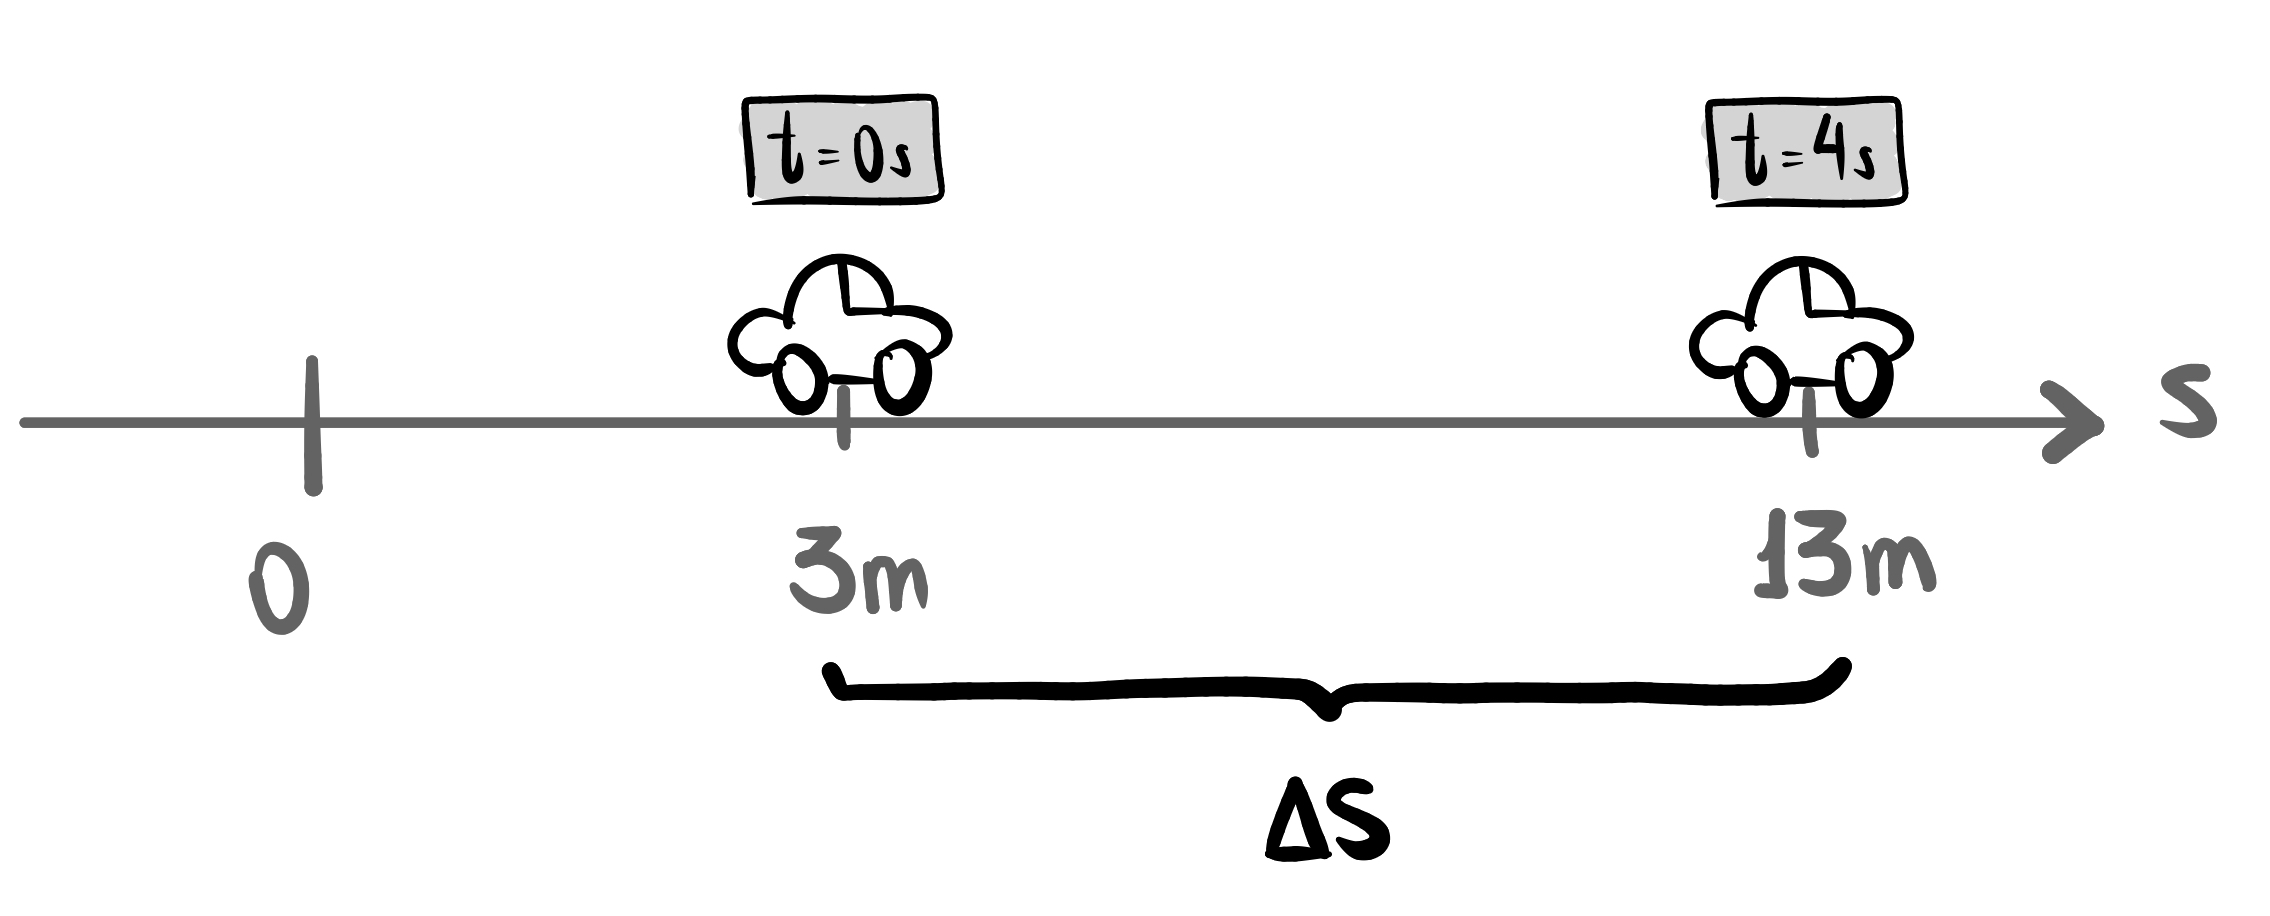
\includegraphics[scale=0.135]{imagensmecanica/deslocamentoescalar.jpeg}
    \caption{Deslocamento $\Delta s.$}
    \label{fig_mec_deslocamento_escalar}
\end{figure}

A bem da verdade, aquela forma de definir a velocidade, feita na introdução, não está exatamente correta -- ou, pelo menos, está incompleta --, por isso vamos refiná-la neste momento. Para medirmos um movimento é preciso que se saiba aonde o objeto está em cada instante de tempo -- é por isso que as estradas possuem placas de quilometragem: caso o seu carro quebre, você pode acionar o guincho e dizer que está no quilômetro 173 da BR-XYZ. 

Em Física, fazemos isso por meio da definição de um eixo de posições $s$, com uma origem -- a posição zero, a partir da qual começamos a medir --, e uma orientação: para onde as posições crescem. A Figura \ref{fig_mec_deslocamento_escalar} mostra isso, em que um carro começa na posição inicial $s_0=3$m, avançando para a posição final $s_f=13$m, ao longo de 4 segundos. A diferença entre a posição inicial e final é o que chamamos de deslocamento escalar $\Delta s$, dado por $\Delta s = s_f - s_0$, e com base nele definimos a velocidade média: ela é a razão entre o deslocamento escalar $\Delta s$ e o intervalo de tempo $\Delta t$ ao longo do qual tal deslocamento acontece.

Dito tudo isso, o leitor poderia se perguntar: \textit{mas isso não é a mesma coisa que a distância?}

E a resposta é: nem sempre. É claro que no caso da Figura \ref{fig_mec_deslocamento_escalar}, as duas coisas coincidem: o carro percorreu uma distância de 10m, e seu deslocamento escalar foi de $\Delta s = s_f-s_0 = 13 - 3 = 10 $m. O deslocamento, da forma como definimos, mede o resultado líquido do movimento, ou, caso o leitor prefira, o efeito global do movimento. A Figura \ref{fig_mec_deslocamento_vs_distancia02} deixa isso mais evidente: ela representa o movimento de um carro que sai da posição inicial $s_0=3$m, se desloca até a posição $13$m e depois retorna até a posição final $s_f=8$m. A distância total percorrida, naturalmente, foi a soma das distâncias varridas na ida e na volta, totalizando $10+5=15$ metros, porém o deslocamento escalar foi $\Delta s = s_f-s_0=8-3=5$ metros.\footnote{Podemos definir a distância percorrida como sendo $d= |\Delta s_{\text{ida}}| + |\Delta s_{\text{volta}}|,$ de modo que a distância percorrida será sempre positiva, diferente do deslocamento.}

Veja que a distância percorrida leva em conta, de fato, o comprimento da trajetória do corpo, enquanto que o deslocamento escalar -- posição final menos inicial -- irá medir o quanto o corpo se afastou do seu ponto de partida, ou seja, o efeito ``líquido do movimento''. Note que em todos os casos nos quais \textbf{não há inversão no sentido do movimento}, ou seja, o objeto sempre avança no mesmo sentido, a distância e o deslocamento escalar irão sempre coincidir -- e boa parte dos movimentos que estudaremos aqui estarão nesse contexto. Ou seja, nesses casos, as Equações \eqref{00intro_eq_velocidade} e \eqref{mecanica_eq_velocidademedia} serão equivalentes. O deslocamento escalar e a distância foram diferentes no caso da Figura \ref{fig_mec_deslocamento_vs_distancia02} justamente pelo fato de que o carro mudou o sentido de seu movimento.

 \begin{figure}[h]
    \centering
    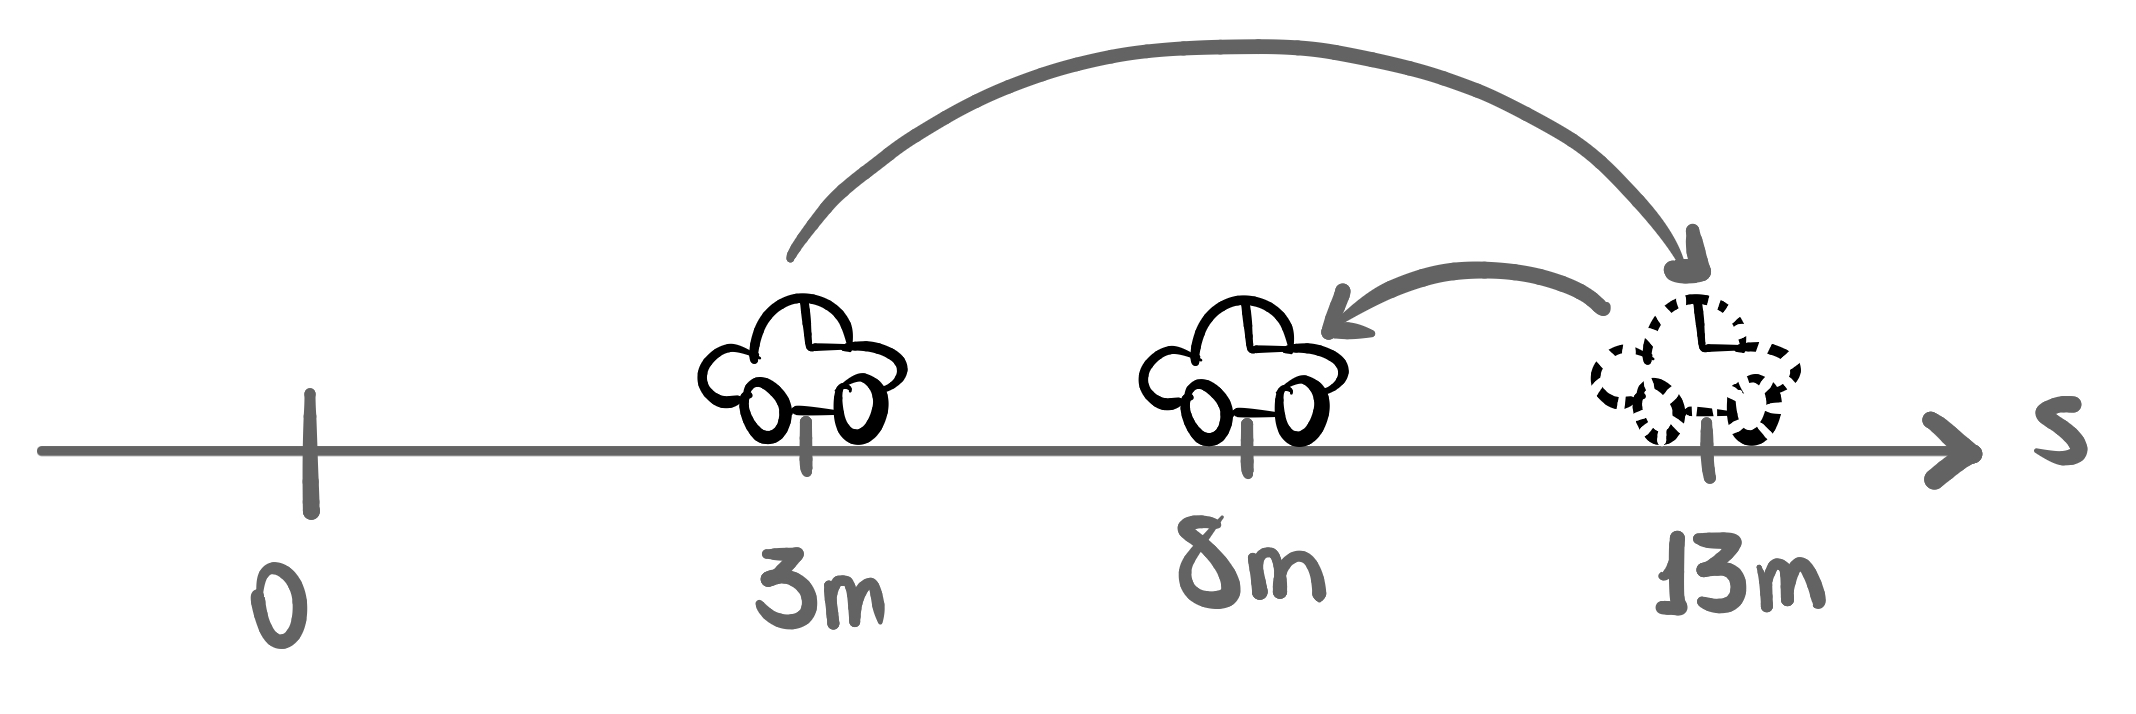
\includegraphics[scale=0.12]{imagensmecanica/deslocamentoescalarn.jpeg}
    \caption{A diferença entre o deslocamento $\Delta s$ e a distância percorrida $d$.}
    \label{fig_mec_deslocamento_vs_distancia02}
\end{figure}


%  \begin{figure}[h]
%     \centering
%     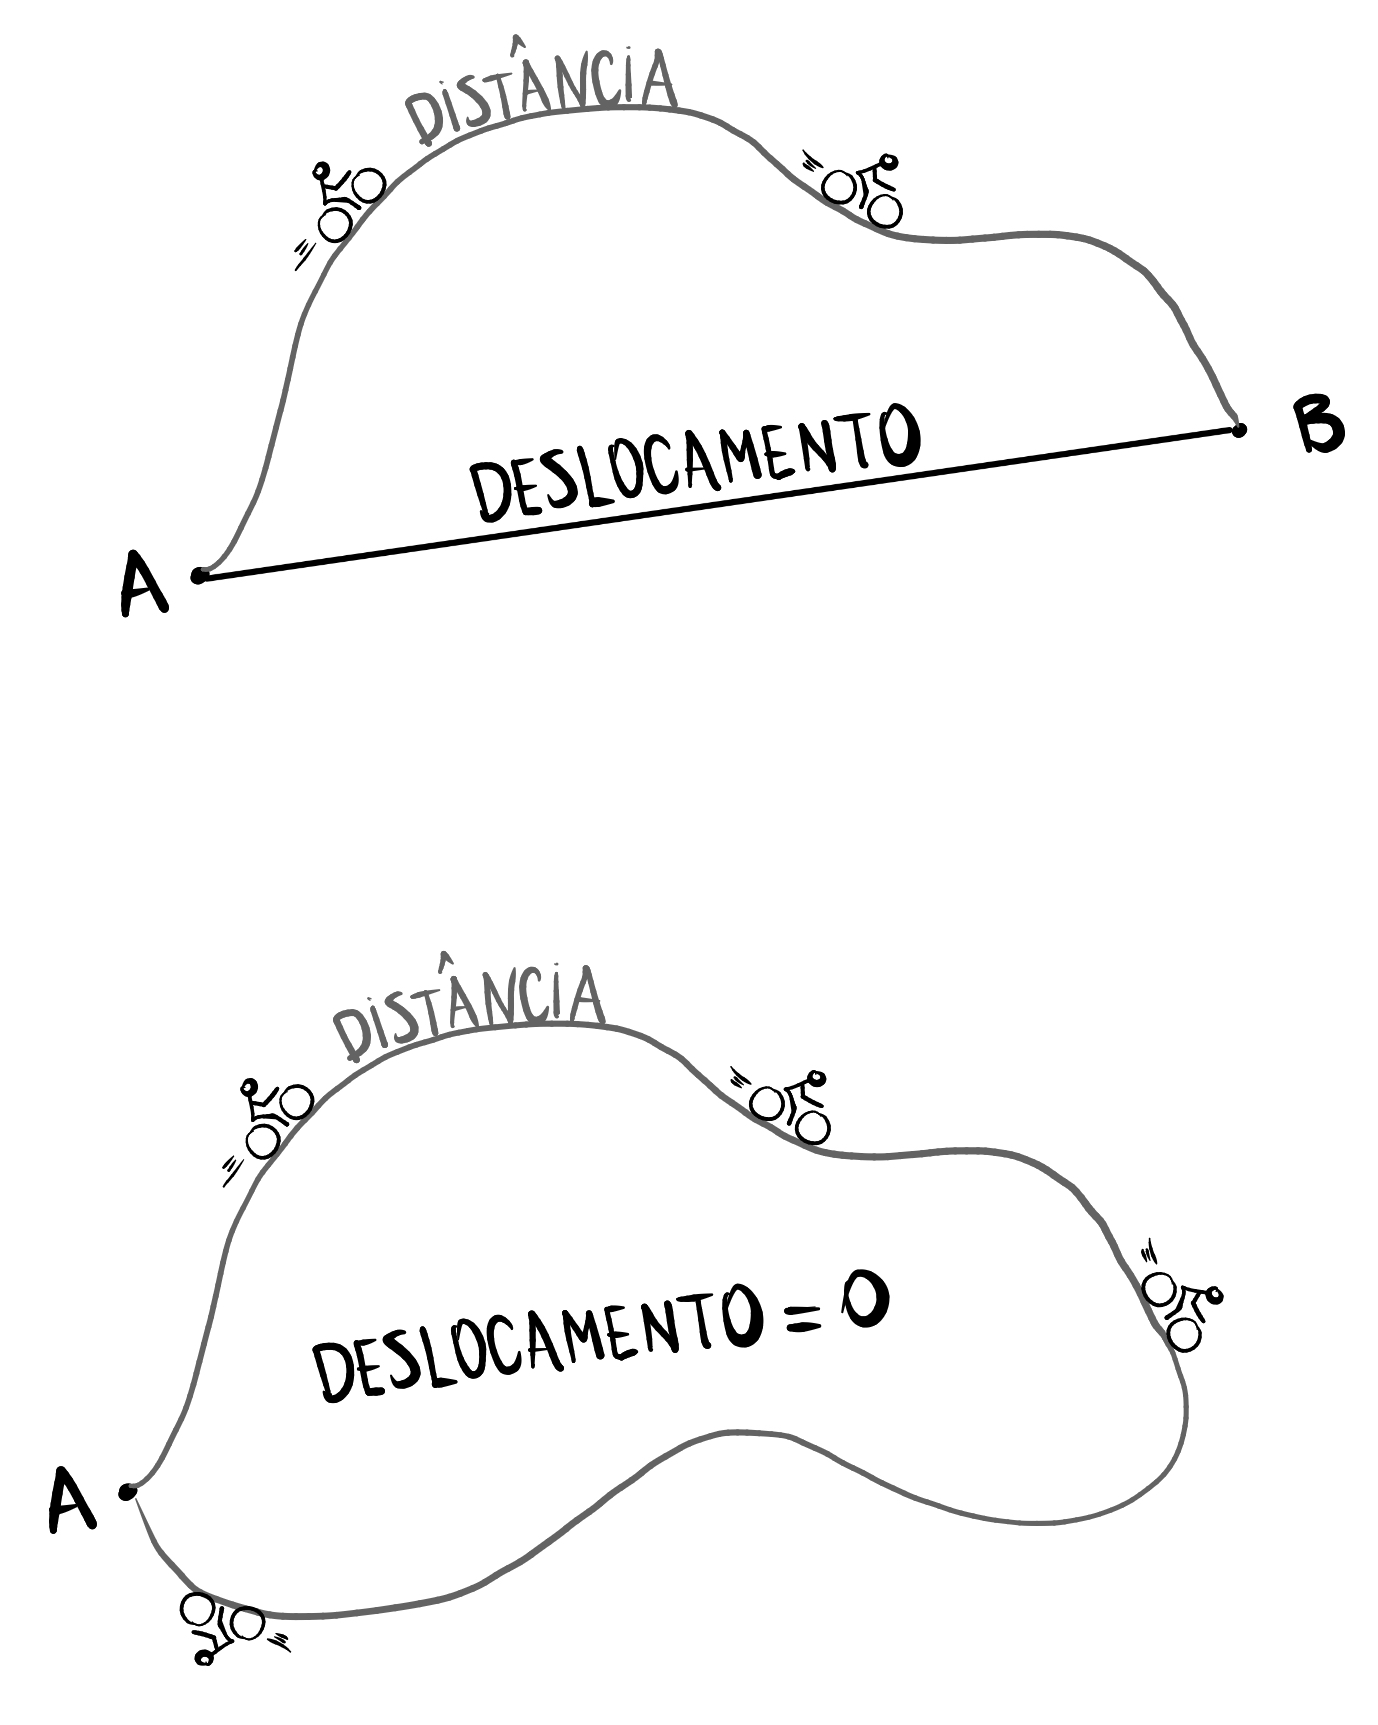
\includegraphics[scale=0.18]{imagensmecanica/deslocamentovsdistancia02.jpeg}
%     \caption{A diferença entre o deslocamento $\Delta s$ e a distância percorrida $d$.}
%     \label{fig_mec_deslocamento_vs_distancia02}
% \end{figure}



Como dito, em vários contextos a distância e o deslocamento irão coincidir. A Figura \ref{fig_mec_deslocamento_vs_distancia02} serve para mostrar um contexto em que isso não ocorre, a fim de deixar clara a diferença entre as duas grandezas.

Agora, a essa altura, o leitor poderia indagar:

\begin{center}
\textit{Ok, até entendi a diferença entre os dois...mas por que a velocidade é definida com base no deslocamento e não na distância?}
\end{center}

Essa, caro leitor, seria uma pergunta deveras inteligente...mas, infelizmente, não temos ferramentas, a essa altura, para respondê-la, de modo que a discussão terá que ficar para um momento futuro.\footnote{Nós poderíamos, inclusive, definir duas grandezas diferentes -- o que de fato ocorre, pelo menos em língua inglesa. Em português não se costuma encontrar isso na literatura, mas em literaturas em língua inglesa é comum que se defina o termo \textit{speed}, ou seja, a rapidez do movimento, como sendo a razão da distância dividida pelo intervalo de tempo. Já o termo \textit{velocity} seria a própria velocidade, que é a razão entre o deslocamento pelo tempo. Como podemos criar conceitos a nosso bel prazer, é possível que tenhamos esses dois conceitos diferentes para medir o movimento: a \textbf{rapidez}, que mede o ``movimento total'', e a \textbf{velocidade}, que mede o ``movimento líquido''. A razão da velocidade, ou seja, de se medir o movimento por meio do deslocamento, ser mais relevante e útil do que a medida do movimento a partir da distância -- o conceito de \textit{speed} -- é o que ficará claro mais adiante.}


Para concluir: na Física, velocidade média não é uma medida de quão longo foi o caminho percorrido, mas de quão diferente é a posição final da posição inicial. Por isso, ela é definida a partir do deslocamento, e não da distância.


\secgfe{Onde é usada}

Como a Cinemática se propõe a estudar o movimento dos corpos, e a velocidade é a grandeza fundamental que mede o movimento, ela aparecerá em absolutamente todas as equações da Cinemática. Além disso, em todas as equações que envolvem o movimento, a velocidade também estará lá. Como um exemplo disso, temos a energia cinética, que é a energia associada ao movimento. Naturalmente, a velocidade irá aparecer em tal equação. Já a força magnética $F_M$ em uma carga elétrica depende do movimento da partícula ao longo do campo, de modo que a velocidade $v$ também irá aparecer em tal equação.

\[
\underbrace{E_c = \frac{1}{2}mv^2}_{\text{Energia cinética}} \quad ; \quad
\underbrace{v^2 = v_0^2 + 2a\Delta s}_{\text{Equação de Torricelli}} \quad ; \quad 
\underbrace{F_M = Bqv\sin\theta}_{\text{Força magnética}} \quad ; \quad
\]


\secgfe{Erros comuns}


\begin{itemize}
    \item [(i)] Considere a Figura \ref{fig_mec_deslocamento_vs_distancia}, que mostra um objeto que sai da posição $s_0=3$ m, se desloca 10m para a direita, e depois retorna 10m para esquerda, terminando na posição $s_f=3$m. Digamos que tal movimento ocorre ao longo de um intervalo de tempo de $5$s. Ora, intuitivamente o leitor poderia pensar:
    
    \textit{Se o objeto percorre uma distância de 20m (10m na ida e 10m na volta) durante 5s, então sua velocidade é $v=\sfrac{d}{t} = \sfrac{20\text{m}}{5\text{s}} = 4$ m/s.} 


    \begin{figure}[h]
    \centering
    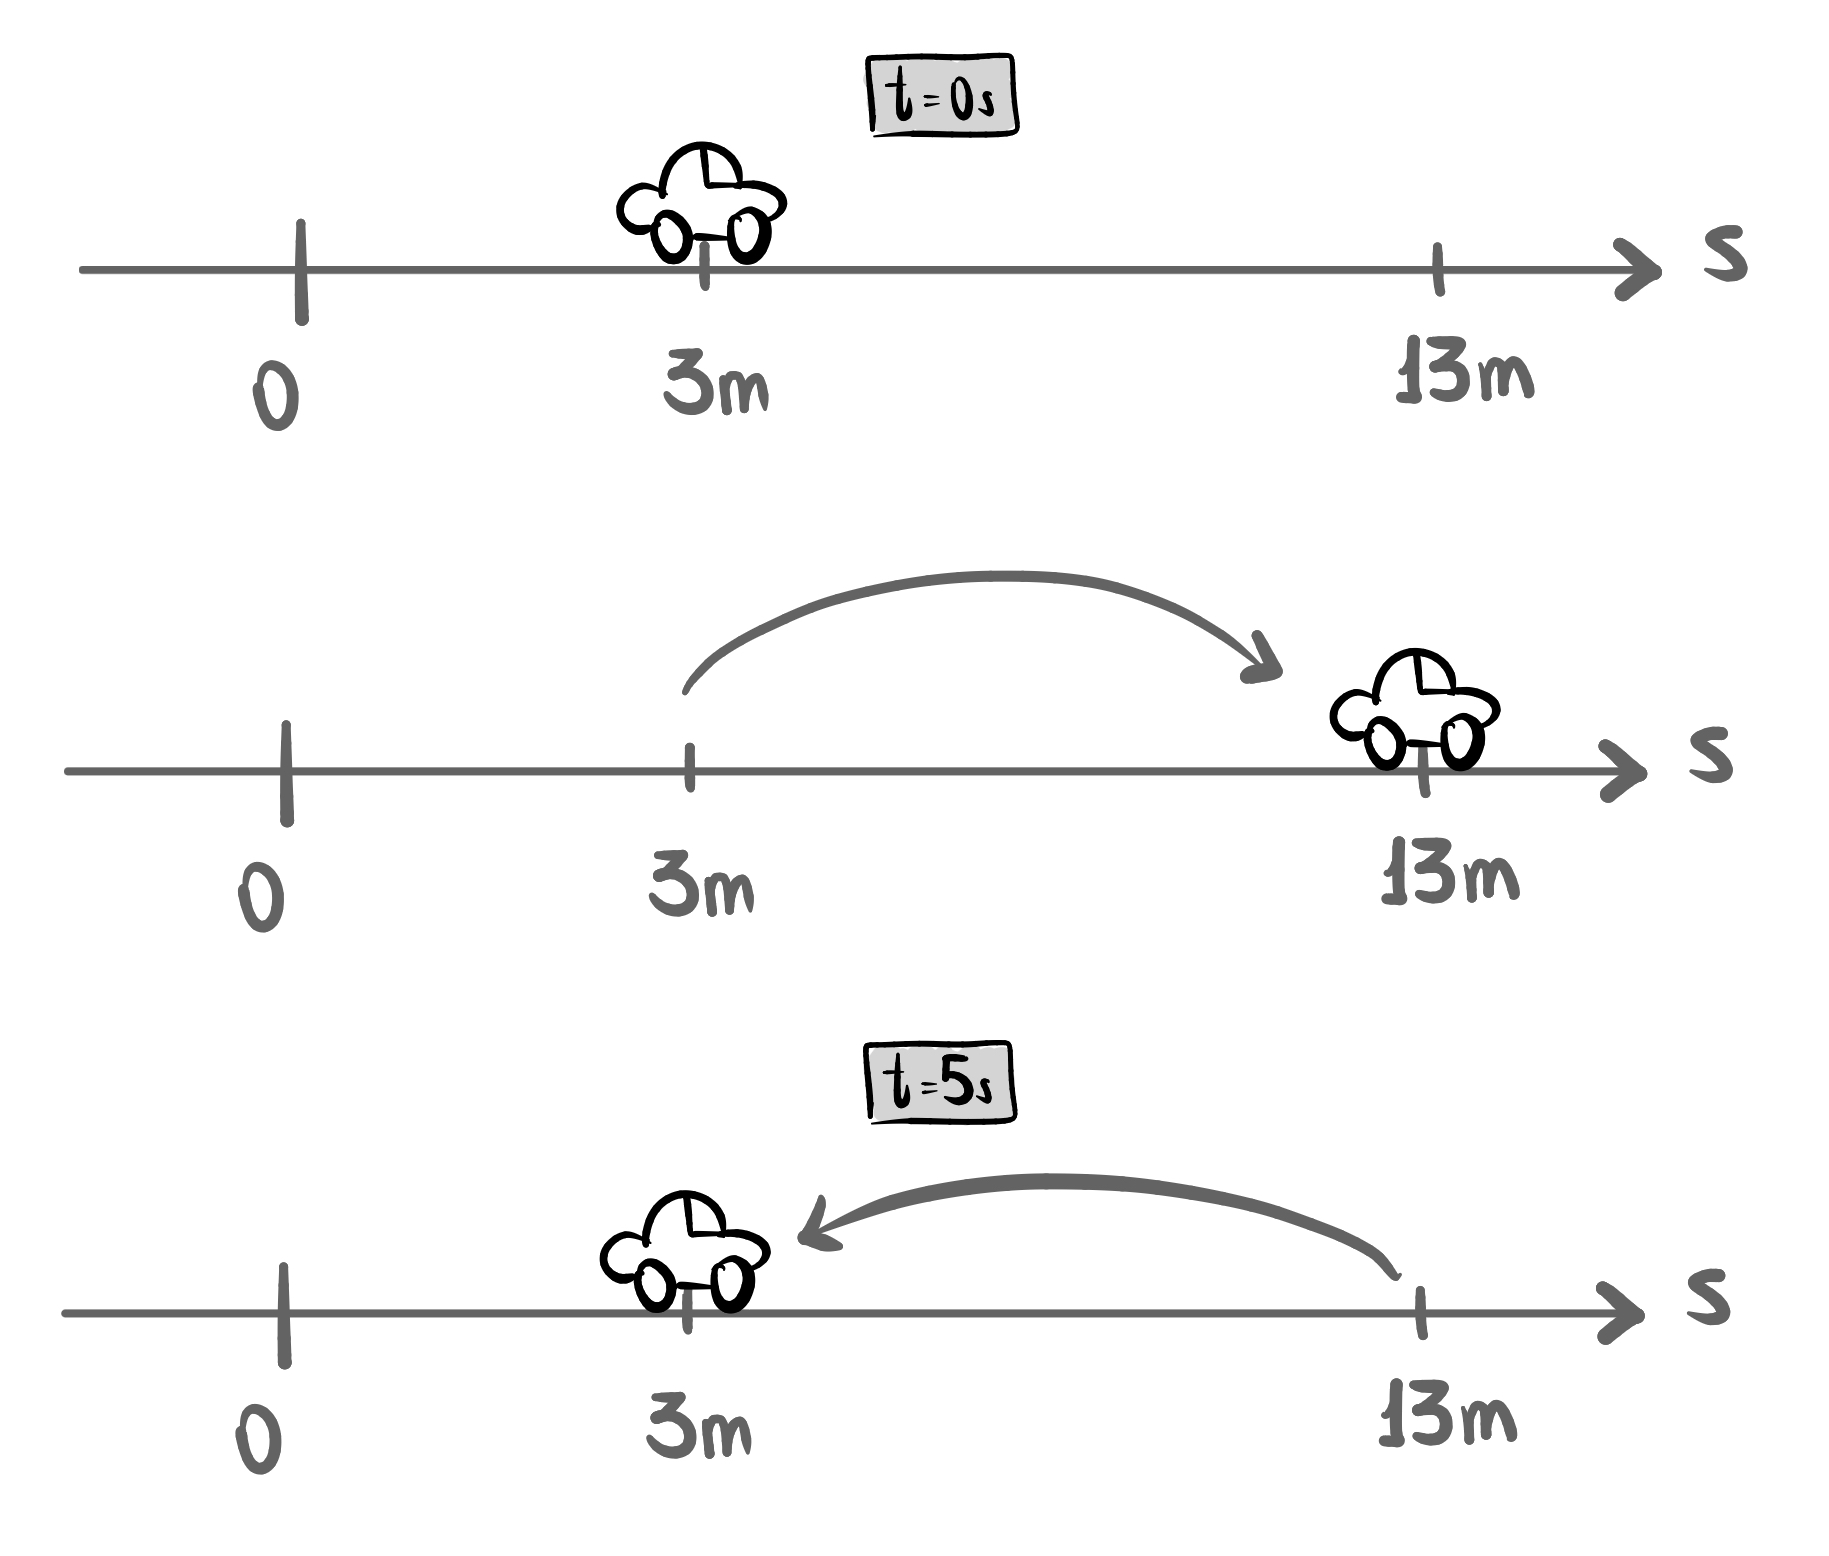
\includegraphics[scale=0.15]{imagensmecanica/deslocamentovsdistanciaescalar.jpeg}
    \caption{A distância percorrida é de 20m, mas o deslocamento, isto é, o quanto o corpo se afastou da sua posição inicial, é nulo.}
    \label{fig_mec_deslocamento_vs_distancia}
\end{figure}

    
    Isso, contudo, estaria errado, segundo a definição feita na Equação \eqref{mecanica_eq_velocidademedia}. A velocidade média neste trecho seria, na verdade, dada por

    $$ v_m = \dfrac{\Delta s}{\Delta t} = \dfrac{s_f-s_0}{t_f-t_0} = \dfrac{3-3}{5 \text{ s}} = 0 \text{ m/s}. $$

    Por mais estranho que isso possa lhe parecer, essa é a definição que fizemos: queremos medir o quanto o objeto se afastou da sua posição inicial e, se ele começa em uma posição e termina na mesma posição, ele não se afastou -- no resultado final de seu movimento -- do seu ponto de partida, de modo que seu deslocamento -- a variação $\Delta s$ da posição -- é nulo, o que resulta em uma velocidade média nula neste trecho, por mais que o objeto tenha se movido ao longo do tempo.

    O erro aqui, portanto, é considerar a distância, e não o deslocamento escalar, para o cálculo da velocidade média.

    \item [(ii)] Considere um carro que sai da cidade A, avança 120 km em 2 horas, e para a fim de abastecer em um posto. O motorista, além de abastecer, resolve fazer um lanche, ficando parado por 1 hora. Em seguida, ele sai do posto, se deslocando por mais 180 km, na mesma direção e sentido, para a cidade B. Se este último trecho é feito em outras 2 horas, qual foi a sua velocidade média ao longo da viagem?


    Existem vários erros diferentes que podem ser cometidos aqui, vamos tentar passar pelos mais comuns.

    \begin{enumerate}
        \item O estudante faz a velocidade média em cada trecho do movimento, e depois faz a média entre elas. Ou seja, no primeiro trecho, da cidade A ao posto, a velocidade média foi de 120km/2h = 60 km/h. No segundo trecho, do posto à cidade B, a velocidade média foi de 180km/2h = 90 km/h. Fazendo a média, teremos
        $$ v_m = \dfrac{60+90}{2} = 75 \text{ km/h.}$$

        Este resultado -- e tal raciocínio -- está totalmente errado. O erro aqui é confundir velocidade média, que é uma grandeza física cujo significado é definido e encapsulado pela Equação \eqref{mecanica_eq_velocidademedia}, com a média aritmética das velocidades. Talvez a confusão seja por tal grandeza levar o termo \textit{média} no nome, mas isso de fato não tem absolutamente nenhuma relação com o cálculo da média aritmética entre números. Tal raciocínio não faz nenhum sentido, haja vista que, pela forma como definimos a velocidade média, o conceito de média aritmética não tem nenhuma relação com a forma como se calcula tal grandeza.

        \item O estudante desconsidera o tempo em repouso, considerando que o carro teve um deslocamento total de $120+180 = 300 $ km, ao longo de um tempo total de movimento de $2+2 = $ 4h, o que daria uma velocidade média, pela definição, de 

        $$ v_m = \dfrac{\Delta s}{\Delta t} = \dfrac{300 \text{ km}}{4 \text{ h}} = 75 \text{ km/h}.$$

        Neste caso, o estudante aplicou a definição corretamente, porém errou na hora mensurar uma das grandezas envolvidas em tal definição. O deslocamento total está correto, é de fato de 300 km. Porém o intervalo de tempo que entra ali é o tempo total de movimento -- desde o carro sair da cidade A até chegar na cidade B, não importando se ele fez pausas no meio do caminho. Por termos desconsiderado o tempo em repouso, chegamos no resultado errado.\footnote{Note que, com este erro, chegamos no mesmo resultado numérico do erro anterior, de 75 km/h. O que foi uma coincidência -- um erro poderia ter nos levado a um valor de velocidade de 75 km/h, enquanto o outro tipo de erro poderia ter nos levado a um valor de 50 km/h, ou qualquer outro. Não se apegue a tal coincidência.}
    \end{enumerate}

O cálculo correto da velocidade média, neste caso, considera o deslocamento total de $120+180 = 300 $ km, ao longo de um intervalo de tempo de $2+2+1 = $ 5h, que é o tempo total de viagem. Isso dá uma velocidade média, pela definição, de 

        $$ v_m = \dfrac{\Delta s}{\Delta t} = \dfrac{300 \text{ km}}{5 \text{ h}} = 60 \text{ km/h}.$$


        O significado disso é o que se segue: um carro que tivesse saído do mesmo local, e se movido durante o mesmo intervalo de tempo total de viagem (5 horas, no caso), com uma velocidade constante de $60$ km/h, teria, ao final das 5 horas, percorrido a mesma distância total.
    
    
\end{itemize}






\secgfe{Observações}


No Sistema Internacional de Unidades de Medida (SI) a unidade padrão para medir distância é metro (m) e a unidade padrão para medir tempo é o segundo (s), de modo que a unidade de medida para velocidade no SI é dada em m/s.

É claro que alguém poderia medir a velocidade em $\text{km}/\text{s}$ ou  $\text{m}/\text{h},$ ou quaisquer outras unidades em que se tem uma unidade de distância no numerador e uma unidade de tempo no denominador. Fora do SI, a unidade mais comum para se medir velocidade é em km/h, de modo que é interessante conhecer a conversão entre tal unidade e aquela do SI, que é dada pela transformação:

\begin{equation}
    \boxed{1 \dfrac{ \text{m}}{\text{s}} = 3,6 \dfrac{\text{km}}{\text{h}}.}
      \label{mecanica_eq_convertermsparakmh}
\end{equation}

Ou seja, em palavras, se você anda 1 metro a cada segundo, você irá percorrer uma distância de 3,6 km ao longo de uma hora. Uma forma intuitiva de lembrar disso é a seguinte: via de regra, uma passada humana varre uma distância de 1 metro. É claro que isso vai variar um pouco para pessoas de diferentes alturas, haja vista que o tamanho da sua perna é o que irá definir o avanço ao longo de uma passada -- mas tal valor, de um metro, é razoável para ser considerado como uma boa média. Dito isso, se você estiver fazendo uma caminhada em ritmo leve, é comum você dar um passo a cada segundo (faça o teste), o que significa que, em tal caminhada -- na qual você avança 1 metro a cada 1 segundo -- você irá percorrer uma distância de 3,6 km se permanecer caminhando ao longo de 1 hora. 

Convido o leitor a fazer o teste e verificar, por si mesmo, que caminhando por 1 hora você avançará uma distância bem próxima de 3,6 km (como dito, o comprimento de suas pernas pode fazer essa distância variar um pouco para cima ou para baixo).

Agora que o leitor possui uma forma empírica de verificar a Equação \eqref{mecanica_eq_convertermsparakmh}, vamos à sua verificação matemática:

$$ 1 \dfrac{\text{km}}{\text{h}} = \dfrac{1000 \text{ m}}{3600 \text{ s}} = \dfrac{1}{3,6} \dfrac{\text{m}}{\text{s}} \implies 1 \dfrac{ \text{m}}{\text{s}} = 3,6 \dfrac{\text{km}}{\text{h}}. $$

Note que usamos que 1 hora possui 3600 segundos (60 minutos, com 60 segundos em cada: $60\cdot 60 = 3600 )$ e que 1 km são 1000 m. O resto são apenas manipulações algébricas.



\vspace{0.3cm}

\begin{exemplo}[Nível I]\label{exemplo_cinematicaescalar_velocidademedia01}

Converta as velocidades abaixo entre m/s e km/h:

\begin{enumerate}
    \item [(a)] 10 m/s
    \item [(b)] 20 m/s
    \item [(c)] 30 m/s
    \item [(d)] 90 km/h
    \item [(e)] 135 km/h
\end{enumerate}


\resolucao


A regra prática que se extrai da Equação \eqref{mecanica_eq_convertermsparakmh} é: se a velocidade está em m/s, multiplica-se tal valor por 3,6 para obtê-la em km/h. Se ela está em km/h, divide-se tal valor por 3,6 para obtê-la em m/s. Faremos isso, como se segue:

\begin{enumerate}
    \item  [(a)] 10 m/s \quad $\xrightarrow{\text{multiplicando por 3,6}} \quad 36 \text{ km/h}.$
    \item  [(b)] 20 m/s \quad $\xrightarrow{\text{multiplicando por 3,6}} \quad 72 \text{ km/h}.$
    \item  [(c)] 30 m/s \quad $\xrightarrow{\text{multiplicando por 3,6}} \quad 108 \text{ km/h}.$
    \item  [(d)] 90 km/h \quad $\xrightarrow{\text{dividindo por 3,6}} \quad 25 \text{ m/s}.$
    \item  [(e)] 135 km/h \quad $\xrightarrow{\text{dividindo por 3,6}} \quad 37,5 \text{ m/s}.$
\end{enumerate}

    
\end{exemplo}





\vspace{0.3cm}

\begin{exemplo}[Nível II (AFA - 2011)]\label{exemplo_cinematicaescalar_velocidademedia02}

Um turista, passeando de bugre pelas areias de uma praia em Natal--RN, percorre uma trajetória triangular, que pode ser dividida em três trechos, conforme a figura abaixo.

{
\centering
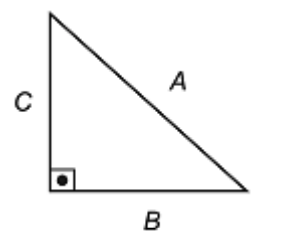
\includegraphics[width=0.2\linewidth]{imagensmecanica/exemplovmedianivel2afa.png}
\captionof{figure}{}
\label{fig_mec_exemplovelocidademedianivel2AFA}
} 


Os trechos $B$ e $C$ possuem o mesmo comprimento, mas as velocidades médias desenvolvidas nos trechos $A$, $B$ e $C$ foram, respectivamente, $v$, $2v$ e $v$. A velocidade escalar média desenvolvida pelo turista para percorrer toda a trajetória triangular vale

\begin{enumerate}
  \item [(a)] $v\sqrt{2}$
  \item [(b)] $2v\sqrt{2}$
  \item [(c)] $4v$
  \item [(d)] $(4 - 2\sqrt{2})\,v$
\end{enumerate}

\resolucao

Seja $x$ o comprimento dos trechos $B$ e $C$, logo, o trecho $A$ possui comprimento $x\sqrt 2.$ Essa é uma boa questão para que o aluno fique atento aos termos. Note que, a rigor, a velocidade escalar média seria nula, haja vista que o deslocamento total foi nulo -- o turista retorna ao mesmo ponto de partida. Contudo, nota-se que não há essa opção nas alternativas, de modo que o estudante atento já deve se dar conta de que houve um deslize conceitual por parte da banca que enunciou a questão. Sendo assim, é fácil induzir que estão tratando da \textit{rapidez} com que o turista se moveu, isto é, a razão entre a distância total percorrida por ele no tempo. \\

Logo, sendo $\Delta t_A$, $\Delta t_B$ e $\Delta t_C$ os tempos necessários para percorrer os trechos $A,$ $B$ e $C,$ respectivamente, teremos que a velocidade média em todo o trecho será

$$ v_m = \dfrac{d_A+d_B+d_C}{\Delta t_A+\Delta t_B+\Delta t_C}=\dfrac{x\sqrt 2+x+x}{\Delta t_A+\Delta t_B+\Delta t_C} = \dfrac{x(2+\sqrt 2)}{\Delta t_A+\Delta t_B+\Delta t_C} .$$

Resta-nos, portanto, obter os tempos de cada trecho:

$$ \Delta t_A=\dfrac{x\sqrt 2}{v}; \quad \Delta t_B=\dfrac{x}{2v}; \quad \Delta t_C=\dfrac{x}{v},$$

\noindent de modo que o tempo total é 

$$\Delta t_A+\Delta t_B+\Delta t_C =  \dfrac{2x\sqrt 2+x+2x}{2v} = \dfrac{x(2\sqrt 2+3)}{2v}, $$

\noindent e, portanto, a velocidade média em todo o trecho foi


$$v_m =\dfrac{x(2+\sqrt2)}{\Delta t_A+\Delta t_B+\Delta t_C} = \cancel{x}(2+\sqrt2) \cdot \dfrac{2v}{\cancel{x}(2\sqrt2+3)} =2v\dfrac{(2+\sqrt2)}{(2\sqrt2+3)},$$

\noindent e, multiplicando por $(3-2\sqrt2)$ o numerador e o denominador para racionalizar, chegamos em

$$  \boxed{ v_m=v(4-2\sqrt2) \implies \text{Letra D.}}$$


    
\end{exemplo}


\vspace{0.3cm}




\begin{exemplo}[Nível III]\label{exemplo_cinematicaescalar_velocidademedia03}

Um móvel desloca-se ao longo de uma trajetória retilínea de comprimento total $L$, dividida em infinitos trechos consecutivos. Em cada trecho o móvel sempre percorre metade da distância restante. Compute a velocidade média do móvel em todo o percurso nos casos em que


\begin{itemize}
  \item [(a)] a velocidade $v$ com que o móvel percorre cada trecho é sempre a mesma.
  
  \item [(b)] a velocidade $v$ com que o móvel percorre cada trecho é sempre a igual à metade da velocidade usada no trecho imediatamente anterior.

  \item [(c)] a velocidade $v$ com que o móvel percorre cada trecho é sempre a igual ao dobro da velocidade usada no trecho imediatamente anterior.
  
\end{itemize}



\resolucao



Nos três casos, note que, ao longo do movimento completo, o deslocamento total (que neste caso coincide com a distância percorrida) do corpo é igual a $L$. Logo, sendo $\Delta t$ o seu tempo total de movimento, teremos que a velocidade média $v_m$ ao longo de todo o movimento será

\begin{equation}
    v_m = \dfrac{\Delta s}{\Delta t} = \dfrac{L}{\Delta t}.
    \label{mecanica_eq_velocidademediaexemplonivelIII}
\end{equation}



O movimento, contudo, é quebrado em infinitas etapas, as quais serão usadas para computar o tempo de cada trecho. Ou seja, o tempo total de movimento $\Delta t$ será quebrado em infinitas partes, cada uma para uma etapa do deslocamento:

$$ \Delta t= \Delta t_1+\Delta t_2+\Delta t_3 + \dots,$$

\noindent em que $\Delta t_i$ representa o intervalo de tempo necessário para o móvel percorrer o $i$-ésimo trecho. Avaliemos cada caso, agora, individualmente.


\begin{itemize}
  \item [(a)] Neste caso a velocidade é sempre $v$, de modo que o tempo de percurso de cada etapa é:

    \begin{enumerate}
        \item [(i)] No primeiro trecho ainda resta a distância total $L$ a ser percorrida, de modo que aqui percorreremos metade deste trecho, o que leva um tempo 

        $$ \Delta t_1 = \dfrac{L/2}{v} = \dfrac{L}{2v}.$$


        \item [(ii)] Agora, no segundo trecho, resta a distância total $L/2$ a ser percorrida, de modo que aqui percorreremos metade deste trecho, o que leva um tempo

        $$ \Delta t_2 = \dfrac{L/4}{v} = \dfrac{L}{4v}.$$


        \item[(iii)]  Resta agora a distância total $L/4$ a ser percorrida, de modo que aqui percorreremos metade deste trecho, o que leva um tempo

        $$ \Delta t_3 = \dfrac{L/8}{v} = \dfrac{L}{8v}.$$
    \end{enumerate}

Já está claro qual é o padrão, de modo que o tempo total de movimento é 
$$\Delta t_A = \dfrac{L}{2v}+\dfrac{L}{4v}+\dfrac{L}{8v}+\dfrac{L}{16v}+\dots  = \dfrac{L}{2v} \left( 1+\dfrac{1}{2} + \dfrac{1}{4} + \dfrac{1}{8}+\dots \right),$$

\noindent em que a soma se estende até o infinito. Note que tal soma é uma progressão geométrica, de termo inicial $a_1=1$ e razão $q=\sfrac{1}{2},$ cuja soma é 

 $$ 1+\dfrac{1}{2} + \dfrac{1}{4} + \dfrac{1}{8}+\dots = \dfrac{a_1}{1-q} = \dfrac{1}{1-\sfrac{1}{2}} = 2,$$

 \noindent logo, o tempo total neste caso é 

 $$ \Delta t_A = \dfrac{L}{2v}\cdot 2 \implies \Delta t_A = \dfrac{L}{v}.$$

 Assim, pela Equação \eqref{mecanica_eq_velocidademediaexemplonivelIII}, a velocidade média neste trecho será

 $$ \boxed{ v_A = \dfrac{L}{\Delta t_A} = \dfrac{L}{L/v} = v}.$$

 Pensando bem, o leitor verá que tal resposta é óbvia: se vamos percorrer o movimento inteiro com a mesma velocidade constante $v$, não importa em quantos trechos o movimento será subdividido -- sendo a velocidade sempre igual a $v$, em qualquer trecho avaliado (seja em apenas um pedaço ou no trecho completo do movimento) a velocidade média será sempre igual a $v.$ \\
 
 Este é um problema baseado no famoso paradoxo de Zenão de Eleia, sobre Aquiles e a Tartaruga. A ideia é que, se dividirmos um movimento finito, como o percurso de uma distância $L$, em infinitas etapas, somos levados a crer que a tarefa nunca será concluída. Contudo, isso é uma inverdade -- é possível varrer infinitas etapas de um processo em um tempo finito, como é o caso aqui, haja vista que a soma dos infinitos tempos é conhecida -- a soma dos infinitos termos de uma P.G. -- e é finita, neste caso. \\

 Desse modo, não era exatamente necessário ter feito todos os cálculos aqui -- de fato era imediato a resposta de que a velocidade média seria $v.$ Contudo, tal desenvolvimento será importante para os próximos itens.
  
  \item [(b)] Note que, neste caso, a velocidade não é constante -- ela assume valores diferentes em cada trecho, de modo que o raciocínio não será tão simples como o anterior. Aqui teremos de fato que avaliar o que ocorre em cada trecho do movimento. Avaliemos cada trecho e o respectivo tempo que leva para percorrê-lo:

   \begin{enumerate}
    \item [(i)] Inicialmente resta a distância total $L$ a ser percorrida, de modo que aqui percorreremos metade deste trecho, com velocidade $v$, o que leva um tempo

    $$ \Delta t_1 = \dfrac{L/2}{v} = \dfrac{L}{2v}.$$


\item [(ii)] Resta-nos agora varrer a distância $L/2$ para concluir o movimento. Neste trecho, percorrer-se-á metade de tal distância, com metade da velocidade anterior, isto é, $v/2,$ o que leva um tempo:

$$ \Delta t_2 = \dfrac{L/4}{v/2} = \dfrac{L}{2v}.$$


\item [(iii)] Resta-nos agora varrer a distância $L/4$ para concluir o movimento. Neste trecho, percorrer-se-á metade de tal distância, ou seja, $L/8$, com metade da velocidade anterior, isto é, $v/4,$ o que leva um tempo:

$$ \Delta t_3 = \dfrac{L/8}{v/4} = \dfrac{L}{2v}.$$

    
\end{enumerate}


A essa altura o leitor já percebeu que o formato para se calcular o intervalo de tempo de duração do $i$-ésimo trecho é do tipo

$$ \Delta t_i = \dfrac{L/2^n}{v/2^{n-1}},$$

\noindent o que sempre resulta em $L/(2v),$ qualquer que seja o valor de $n \geq 1.$


Logo, o tempo total de movimento seria

$$ \Delta t_B =  \Delta t_1+\Delta t_2+\Delta t_3 + \dots= \dfrac{L}{2v}(1+1+1+1+\dots)= \infty,$$

\noindent de onde concluiríamos que a velocidade média, dada por $v_C = L/\Delta t$, tende a zero. O que aconteceu aqui? \\

Talvez o leitor tenha estranhado, mas está tudo normal. É impossível percorrer o trecho de comprimento $L$ da forma como proposto, por isso chegamos em tal resposta: a nossa partícula, na verdade, nunca termina de percorrer o comprimento $L$ inteiro.

Isso acontece porque, em cada novo trecho, apesar de termos que percorrer metade da distância, faremos isso com metade da velocidade, de modo que levaremos o mesmo tempo. Assim, é como se eu te dissesse: \textit{vou fazer infinitas caminhadas, cada uma durando 10 minutos. Quanto tempo levo para terminar tal tarefa?}. \\

Ora, são infinitas etapas com um tempo de duração de 10 minutos -- que seria o nosso $L/(2v)$ --, logo, o tempo total é infinito e a tarefa nunca é concluída. É diferente de quando percorremos metade da distância remanescente mantendo a mesma velocidade, pois isso faz com que o tempo para cumprir cada nova etapa seja cada vez menor, o que pode possibilitar que a soma desses infinitos intervalos de tempo seja finita, como foi o caso do item anterior.


  \item [(c)] Neste caso a velocidade também não é constante, assumindo valores diferentes em cada trecho. Vamos tentar construir uma intuição antes de fazer os cálculos. 

  Perceba que, a cada novo trecho, a distância percorrida diminui -- é sempre metade da distância anterior --, porém agora a velocidade com que se percorre essa distância aumenta -- é sempre o dobro da velocidade do trecho anterior. Assim, o tempo necessário para percorrer cada trecho vai ficando cada vez menor: percorreremos distâncias cada vez menores com velocidades cada vez maiores. Isso deve nos levar a crer que, diferente do item anterior, a soma dos infinitos intervalos de tempo de cada trecho, aqui, deve ser finita, uma vez que os intervalos de tempo ficam cada vez menores. \\

  Indo além, seria razoável esperar, inclusive, que o tempo total neste caso seja menor do que o tempo necessário para varrer a distância $L$ no item $(a),$ uma vez que lá as etapas são feitas sempre com a mesma velocidade $v$, enquanto aqui as novas etapas são feitas com velocidades cada vez maiores, resultando em intervalos de tempo que vão ficando ainda mais curtos do que aqueles que apareciam no caso do item $(a).$ \\

  O leitor pode verificar, neste caso, que a solução será bem semelhante ao do item $(a),$ resultando em um progressão geométrica análoga, porém com razão $q=\sfrac{1}{4}$ -- a distância percorrida em um novo trecho cai pela metade, porém a velocidade com que ele é percorrido dobra, por isso o fator $\sfrac{1}{2^2}$ aparece aqui, e apenas $\sfrac{1}{2}$ no item $(a)$. Assim, o tempo total de movimento é

  $$ \Delta t = \dfrac{L}{2v} \left(1+\dfrac{1}{4}+\dfrac{1}{16}+\dots \right) = \dfrac{L}{2v} \left( \dfrac{a_1}{1-q} \right) = \dfrac{L}{2v}\left( \dfrac{1}{1-\sfrac{1}{4}} \right) =  \dfrac{2L}{3v},$$

\noindent o que resulta, pela Equação \eqref{mecanica_eq_velocidademediaexemplonivelIII}, em uma velocidade média

$$ \boxed{ v_C = \dfrac{L}{\Delta t_C} = \dfrac{L}{\sfrac{2L}{3v}} = \dfrac{3v}{2}.}$$

Para chegar nessa resposta o leitor poderia ter tomado um caminho diferente e raciocinar apenas por comparação com o item $(a):$ no contexto do item $(c)$, em cada trecho, o tempo para percorrê-lo será exatamente metade do tempo para percorrer o mesmo trecho no contexto do item $(a);$ logo, o tempo total de movimento aqui será metade daquele, fazendo com que a velocidade média aqui -- uma vez que a distância total é a mesma -- seja o dobro daquela. Logo, concluiríamos que $v_C = 2v,$ e erraríamos em 33\% a resposta, haja vista que o valor correto é $v_C=1.5v$ \\

O leitor consegue perceber qual é o erro em tal raciocínio? \footnote{Vou dar uma dica para que o leitor possa refletir. Contudo, é importante que as palavras que se seguem sejam lidas apenas após o estudante colocar uma energia mínima em tentar descobrir por si só. Note que existe um único trecho -- o primeiro -- em que o raciocínio aplicado não caberia. No primeiro trecho do movimento -- o percurso de $L/2$, metade da distância total -- os tempos de percurso nos itens $(a)$ e $(c)$ são os mesmos. E por que será que uma diferença de apenas um trecho, entre infinitos, é capaz de gerar uma resposta que diverge em 33\% da resposta correta...?}
  
\end{itemize}





\end{exemplo}

\vspace{0.3cm}







\begin{secnivel}[Velocidade Relativa]{I}{Velocidade Relativa}
  
  \eqLdois{def}{mecanica_eq_velocidaderelativa}{v_{AB} = v_A \pm v_B}

\end{secnivel}








\secgfe{De onde vem}
 
A Equação \eqref{mecanica_eq_velocidaderelativa} nos permite obter a velocidade relativa $v_{AB}$ do objeto $A$ em relação ao objeto $B$. Mas o que raios seria uma velocidade relativa?

Giordano Bruno, contemporâneo de Galileu e coaduno de suas ideias a respeito da astronomia, escreveu, em sua obra \textit{De l’infinito, universo e mondi} de 1584 que

\begin{quote}
    “Nada está absolutamente imóvel; o movimento e o repouso existem apenas por comparação.”
\end{quote}


Essa ideia contém, com profundidade, um dos princípios mais importantes da teoria do movimento galileana: a ideia de que todo movimento é relativo. Para compreender melhor tal conceito, considere a Figura \ref{fig_mec_galileurepousoemovimento01}, que mostra dois indivíduos, Aristóteles, representado pela letra $A$, e Bohr, representado pela letra $B.$ O tempo passa e, aparentemente, nada acontece: a distância entre Aristóteles e Bohr não se altera, de modo que parece razoável que qualquer um conclua que os dois indivíduos estão em repouso.

Contudo, a Figura \ref{fig_mec_galileurepousoemovimento01} não contém toda a realidade do movimento: Aristóteles e Bohr estão, na verdade, no salão de um grande navio, que está viajando pelo oceano pacífico.

{
\centering
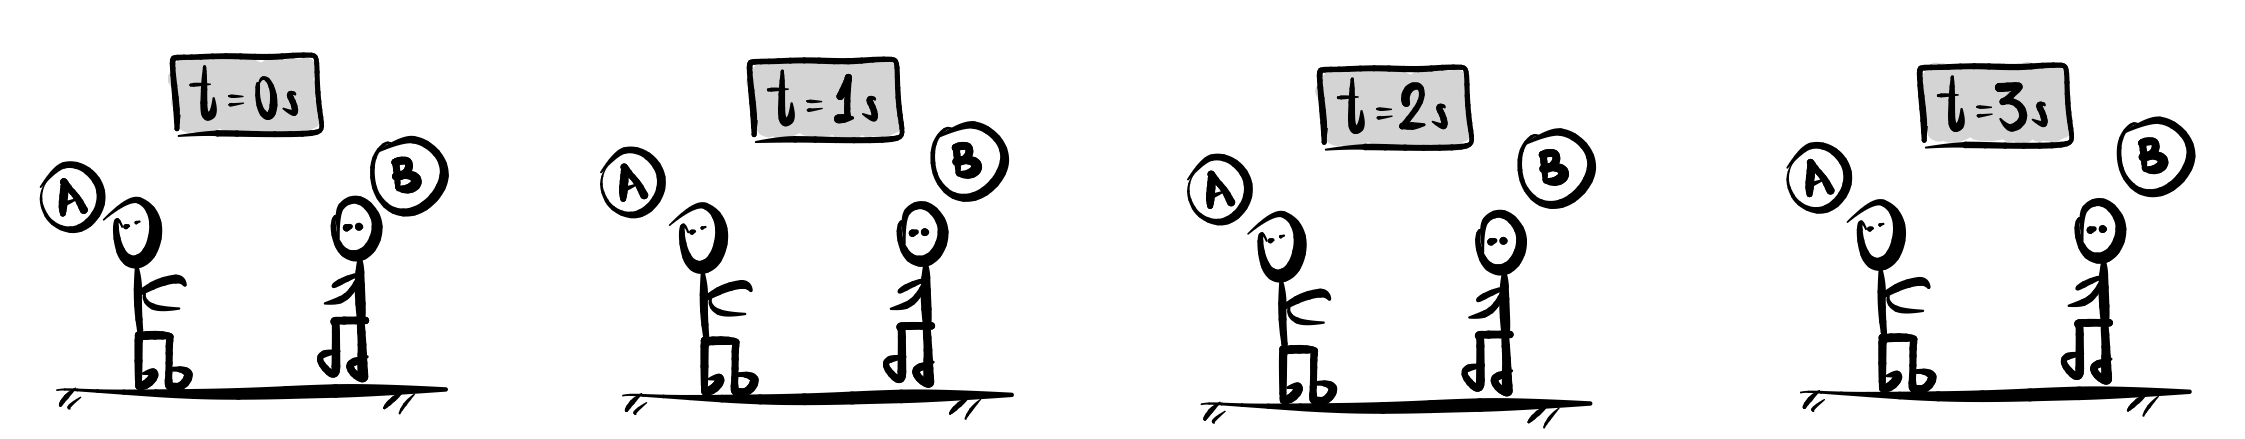
\includegraphics[width=0.9\linewidth]{imagensmecanica/galileu_movimentoerepouso1.jpeg}
\captionof{figure}{Os indivíduos $A$ e $B$ aparentam estar em repouso. }
\label{fig_mec_galileurepousoemovimento01}
} 

A Figura \ref{fig_mec_galileurepousoemovimento02} mostra, gradativamente, tal situação, à medida que vamos dando um \textit{zoom out} na nossa imagem. Note que, à medida que vamos nos afastando, percebemos um terceiro indivíduo, Copérnico, representado pela letra $C$, que aparece em terra firme, observando o navio se mover. Note que, para Copérnico, os indivíduos $A$ e $B$ não estão em repouso: eles se afastam de Copérnico, com a mesma velocidade na qual o navio se move. 

{
\centering
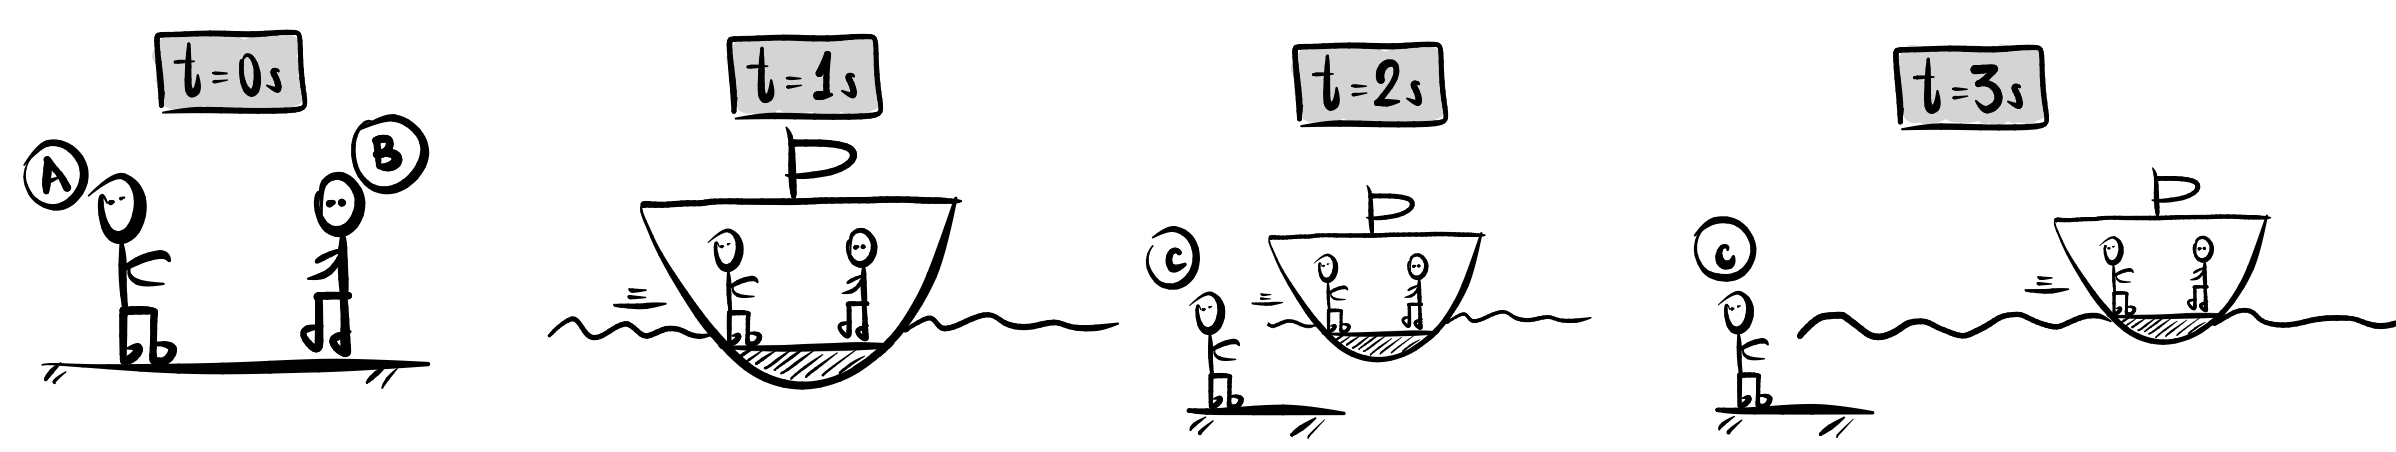
\includegraphics[width=1.0\linewidth]{imagensmecanica/galileu_movimentoerepouso2.jpeg}
\captionof{figure}{Os indivíduos $A$ e $B$ na verdade estão dentro de um navio, que se move em relação ao indivíduo $C.$}
\label{fig_mec_galileurepousoemovimento02}
} 

De modo concreto, caso a velocidade do navio (em relação à terra) seja de $50$ km/h, Copérnico perceberá seus amigos Aristóteles e Bohr se distanciando de si de $50$ km a cada hora que passa. Nesse sentido, seria correto escrever que

$$ v_{AB} = 0,$$

\noindent ou seja, a velocidade de Aristóteles ($A$) em relação à Bohr ($B$) é nula -- um não se move em relação ao outro, o que se evidencia na Figura \ref{fig_mec_galileurepousoemovimento01}. Contudo, não poderíamos dizer que $v_{AC}=0,$ ou seja, como mostra a Figura  \ref{fig_mec_galileurepousoemovimento02}, Aristóteles não está parado em relação à Copérnico, eles se afastam um do outro de 50 km a cada hora, ou seja:

$$ v_{AC}=50 \text{ km/h.}$$



Perceba, portanto, que a pergunta \textit{``qual é a velocidade de Aristóteles?''} não faz sentido. Essa pergunta só faz sentido quando, primeiro, fixarmos um referencial -- em relação a quem tal velocidade é medida. Do contrário, a velocidade Aristóteles pode ser qualquer valor: ela é zero para alguns, $50$ para outros, $120$ para alguns outros, e por aí vai.

É nesse sentido que foi afirmado, no início da seção, que \textbf{toda velocidade é relativa.} Não existe nenhuma grandeza física que se chama ``a velocidade de Aristóteles,'' como se essa fosse uma propriedade única e absoluta, que dependesse apenas de Aristóteles. O que existe é a velocidade de Aristóteles em relação à Bohr, representada por $v_{AB,}$ ou a velocidade $v_{AC}$ de Aristóteles em relação à Copérnico; ou a velocidade de $v_{AD}$ de Aristóteles em relação à Diofanto, e por aí vai. Ou seja, retomando as palavras de Giordano Bruno: \\


\begin{center}
   \textit{\textbf{``...o movimento e o repouso existem apenas por comparação.''}} 
\end{center}

Perceba, portanto, que quase sempre o enunciado de um problema de Física acaba cometendo um certo abuso de linguagem, quando ele diz que \textit{``considere um carro, cuja velocidade é de $60$ km/h, que se move e persegue um outro carro...''}. Não existe nenhum carro com a propriedade absoluta de ter $60$ km/h de velocidade -- essa velocidade é em relação a algum referencial, e terá outro valor em relação a outros referenciais. Contudo, nesses contextos, fica-se subentendido que nosso laboratório de análise é a Terra, de tal modo que tal velocidade é em relação à Terra. Ou seja, em relação a um indivíduo que está parado sobre este planeta, por exemplo, em frente à rodovia pela qual o carro passa. Desse modo, sempre que em algum contexto for informada uma velocidade sem informar explicitamente qual é o referencial no qual aquela velocidade é medida, assume-se que tal referencial é a terra.

Toda essa digressão parece uma grande conversa fiada, mas ela é absolutamente necessária. Agora que entendemos que toda velocidade é relativa -- que o movimento e o repouso só existem por comparação -- estamos prontos para fazer a pergunta: se soubermos a velocidade $v_{AT}$ de Aristóteles em relação à Terra, e a velocidade $v_{BT}$ de Bohr em relação à Terra, como podemos obter a velocidade $v_{AB}$ de Aristóteles em relação à Bohr? Esse é o problema que a Equação \eqref{mecanica_eq_velocidaderelativa} se propõe a resolver.

Perceba, portanto, que o problema de se calcular uma velocidade relativa é, na verdade, um problema de mudança de referencial: temos a velocidade $v_{AT}$ de Aristóteles em relação à Terra e queremos saber a velocidade $v_{AB}$ de Aristóteles em relação à Bohr. Sempre que você estiver obtendo uma velocidade relativa você estará, no fundo, operando uma mudança de referencial: obtendo a velocidade do corpo em relação a algum outro, ou seja, no referencial deste algum outro -- na perspectiva dele. Comecemos por entender o que significar observar algo na perspectiva de um certo referencial, digamos o referencial $A$ - Aristóteles. \\

O leitor há de concordar comigo que é impossível que Aristóteles se mova em relação a si mesmo, certo? Se ele andar 10 metros para a direita, adivinhe: lá ele estará. Se ele se mover 4 metros para cima, lá ele estará. Parece meio óbvio isso, mas será um conceito importante para a nossa construção: um corpo nunca se move em relação a si mesmo. 
\begin{center}
    \textit{``Ah, tenho um amigo que tomou uma certa substância e disse que sua alma saiu do corpo.''} 
\end{center}

Bom, estamos falando de física aqui, e não de alucinações. No contexto físico, é impossível que um objeto se mova em relação a si mesmo, uma vez que, para onde ele for, lá ele estará -- ele não se distancia nunca de si mesmo.

Dito isso, estudar um problema na perspectiva de Aristóteles é avaliar o problema no referencial no qual Aristóteles está parado, haja vista que, do ponto de vista de Aristóteles, ele está sempre parado -- ele nunca se move em relação a si mesmo. Este é o primeiro grande e importante passo para construirmos a Equação \eqref{mecanica_eq_velocidaderelativa}.


O segundo passo está relacionado à balança de pratos da Figura \ref{fig_mec_balanca01}. Note que ela está, na primeira imagem, em equilíbrio, com 2 pesos de cada lado. Caso alguém adicione um peso em apenas um dos lados a configuração inicial da balança irá, naturalmente, ser modificada, como mostra a imagem do meio. Contudo, se adicionarmos um peso do lado esquerdo mas fizermos exatamente a mesma coisa do lado direito, então a configuração inicial não é afetada -- a situação física permanece a mesma.


{
\centering
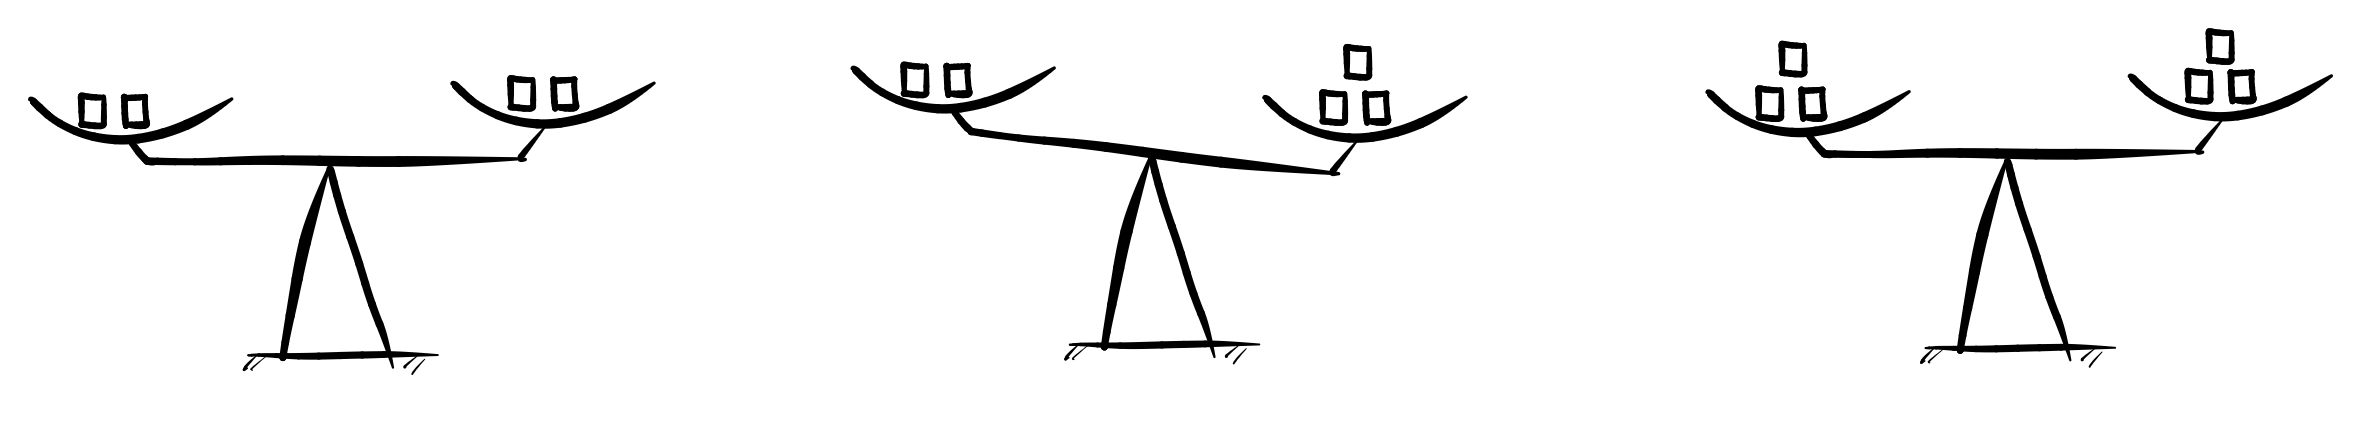
\includegraphics[width=0.8\linewidth]{imagensmecanica/balancapratos01.jpeg}
\captionof{figure}{A balança permanece em equilíbrio caso se adicione a mesma quantidade dos dois lados.}
\label{fig_mec_balanca01}
} 
\vspace{0.3cm}

Perceba que isso é verdade independente da balança estar ou não em equilíbrio, como é mostrado na Figura \ref{fig_mec_balanca02}, para uma balança inicialmente desequilibrada, com 2 pesos do lado direito e apenas 1 do lado esquerdo. Se adicionarmos 1 peso de um lado e nenhum do outro, então a configuração inicial da balança certamente será perturbada, como mostra a imagem do centro de tal figura. Contudo, se, mais uma vez, adicionarmos a mesma quantidade dos dois lados da balança, então a configuração inicial não é alterada, como o leitor pode perceber comparando a primeira e a última imagem da Figura \ref{fig_mec_balanca02}.
\vspace{0.3cm}

{
\centering
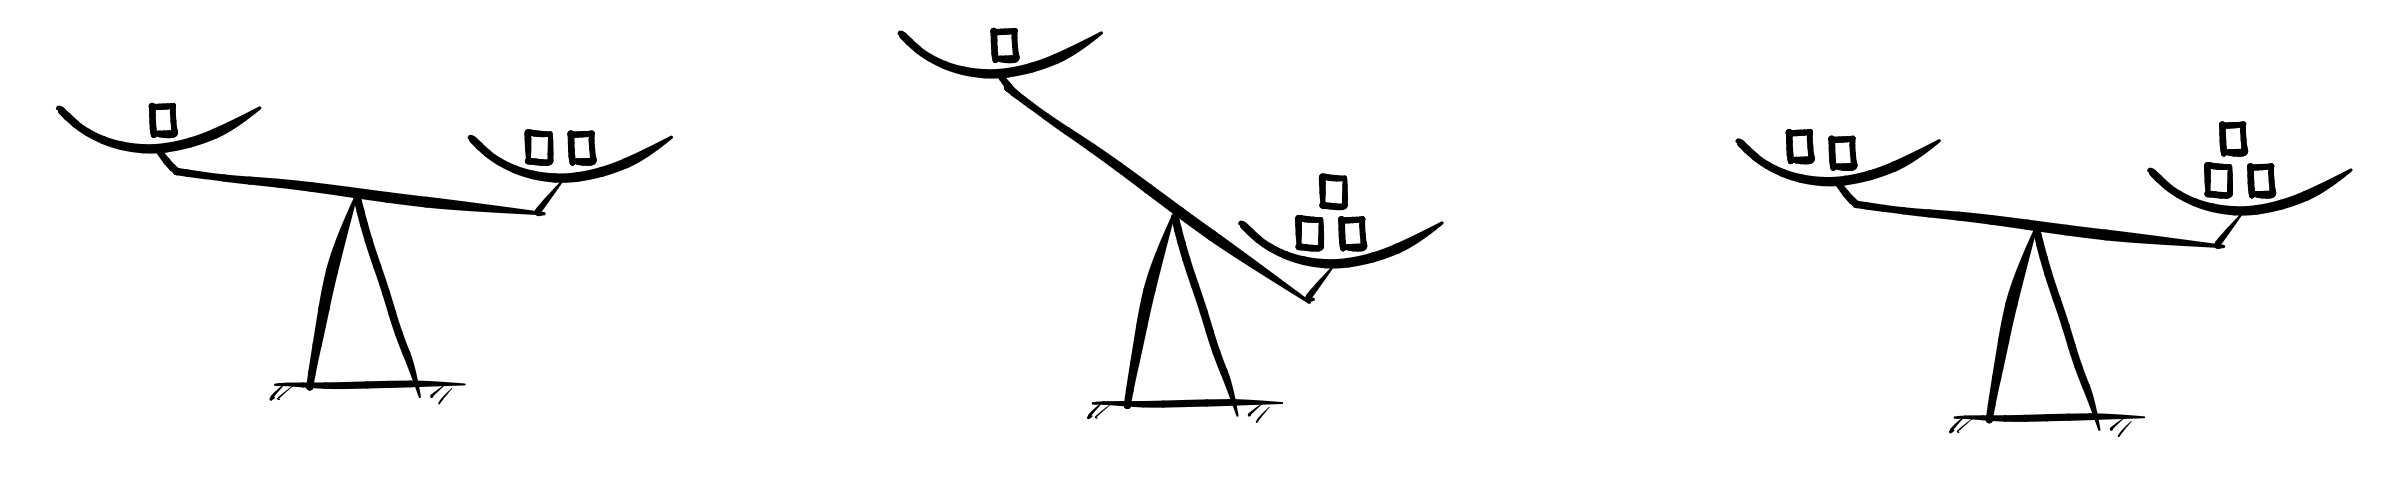
\includegraphics[width=0.8\linewidth]{imagensmecanica/balancapratos02.jpeg}
\captionof{figure}{A balança permanece na mesma configuração inicial caso se adicione a mesma quantidade dos dois lados.}
\label{fig_mec_balanca02}
} 

Sim, caro leitor -- a nossa conversa não tem absolutamente nada a ver com balanças. A ideia aqui é apenas usar esta analogia para extrair um princípio que utilizaremos aqui: em alguns contextos físicos, se adicionarmos a mesma quantidade a todos os elementos deste contexto -- no caso, os pratos da balança -- a física não é alterada, isto é, o sistema não é perturbado ou modificado.

Vamos agora ao nosso problema: Aristóteles está de carro, se movendo para a direita com uma velocidade $v_A=20$ m/s, enquanto Bohr se move em sentido contrário, com velocidade $v_B=30$ m/s.


{
\centering
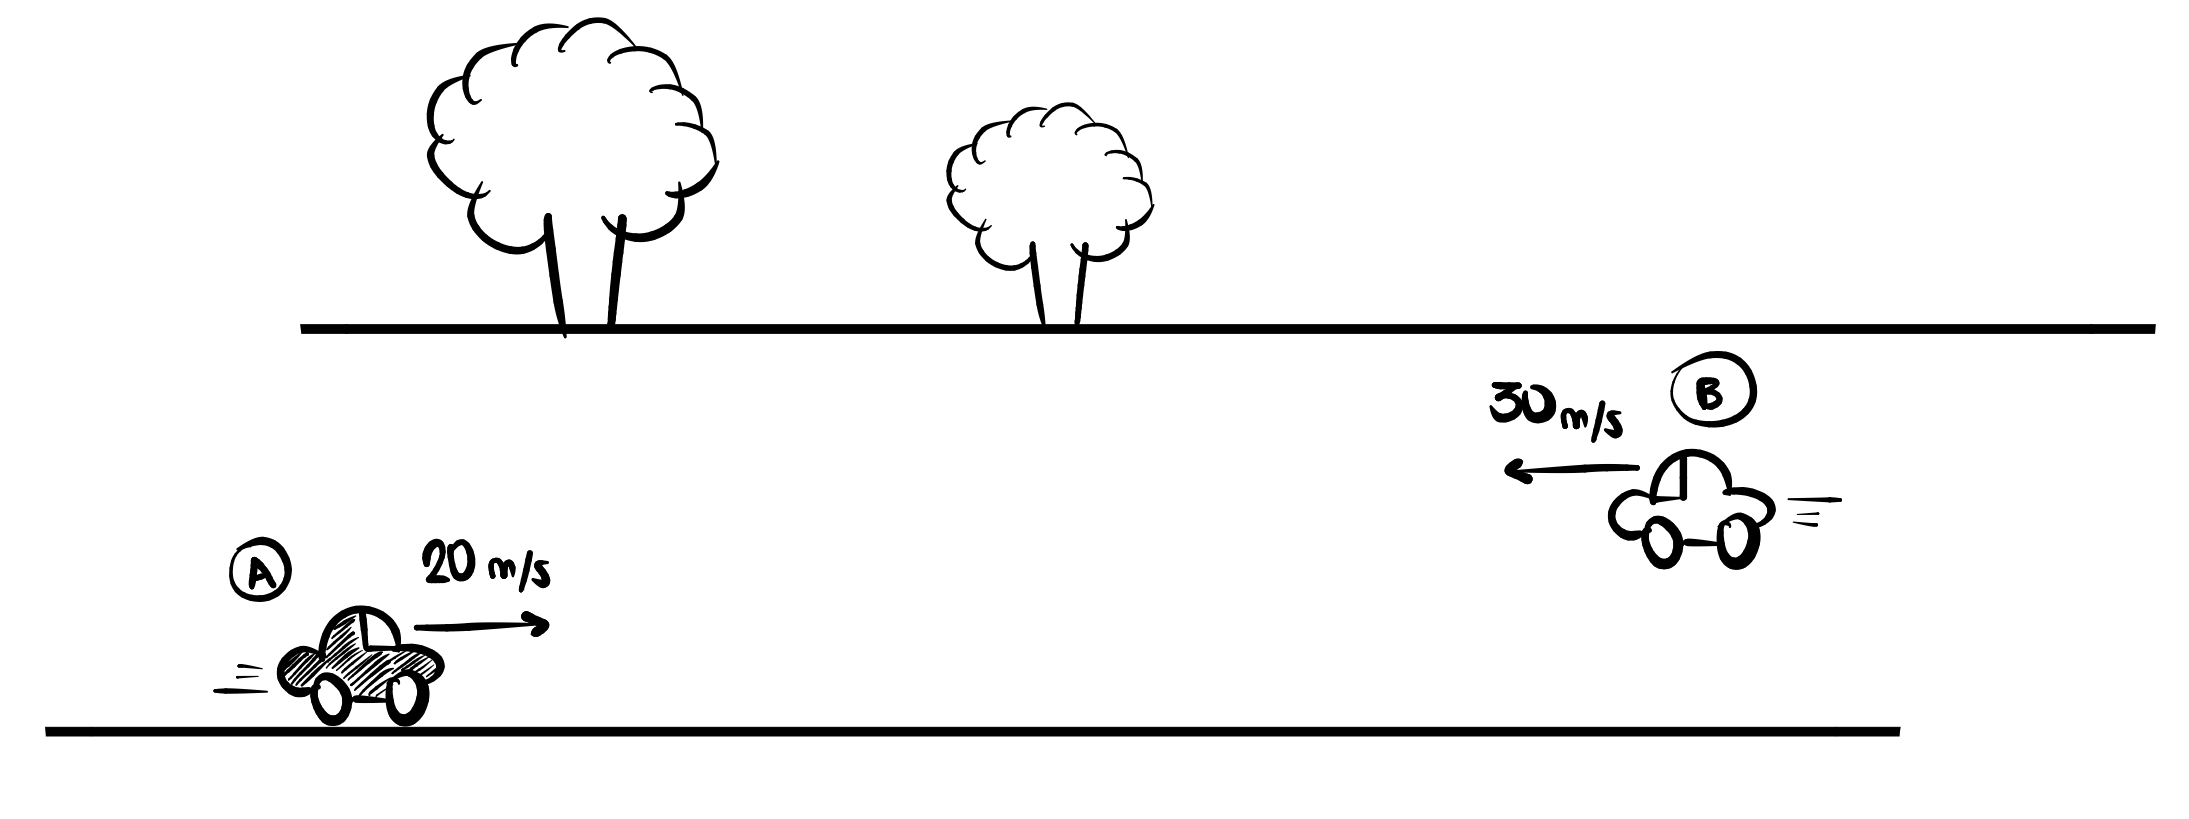
\includegraphics[width=0.6\linewidth]{imagensmecanica/velrelativaemudancaderefAB1.jpeg}
\captionof{figure}{Velocidades de $A$ e $B$ no referencial das árvores (terra).}
\label{velrelativaemudancaderefAB1}
} 
\vspace{0.3cm}

Note que não foi especificado em relação a qual referencial tais velocidades são medidas, de modo que assumimos que se trata da terra, como mostra a Figura \ref{velrelativaemudancaderefAB1}. Digamos que nosso interesse é o de obter a leitura do contexto no referencial de Bohr, ou seja, no referencial no qual $B$ está parado. Ora, para parar o carro $B$, que se move a $30$ m/s para a esquerda, o natural seria adicionar nele uma velocidade de $30$ m/s para a direita, o que anularia a sua velocidade e o colocaria em repouso. 

Contudo, fazer isso alteraria a configuração da nossa ``balança'', de modo que, para que sejamos justos, devemos adicionar a mesma coisa a todos os elementos do sistema; ou seja: adicionaremos uma velocidade de $30$ m/s para a direita a todos os corpos do nosso sistema, como mostra a Figura \ref{velrelativaemudancaderefAB2}.

{
\centering
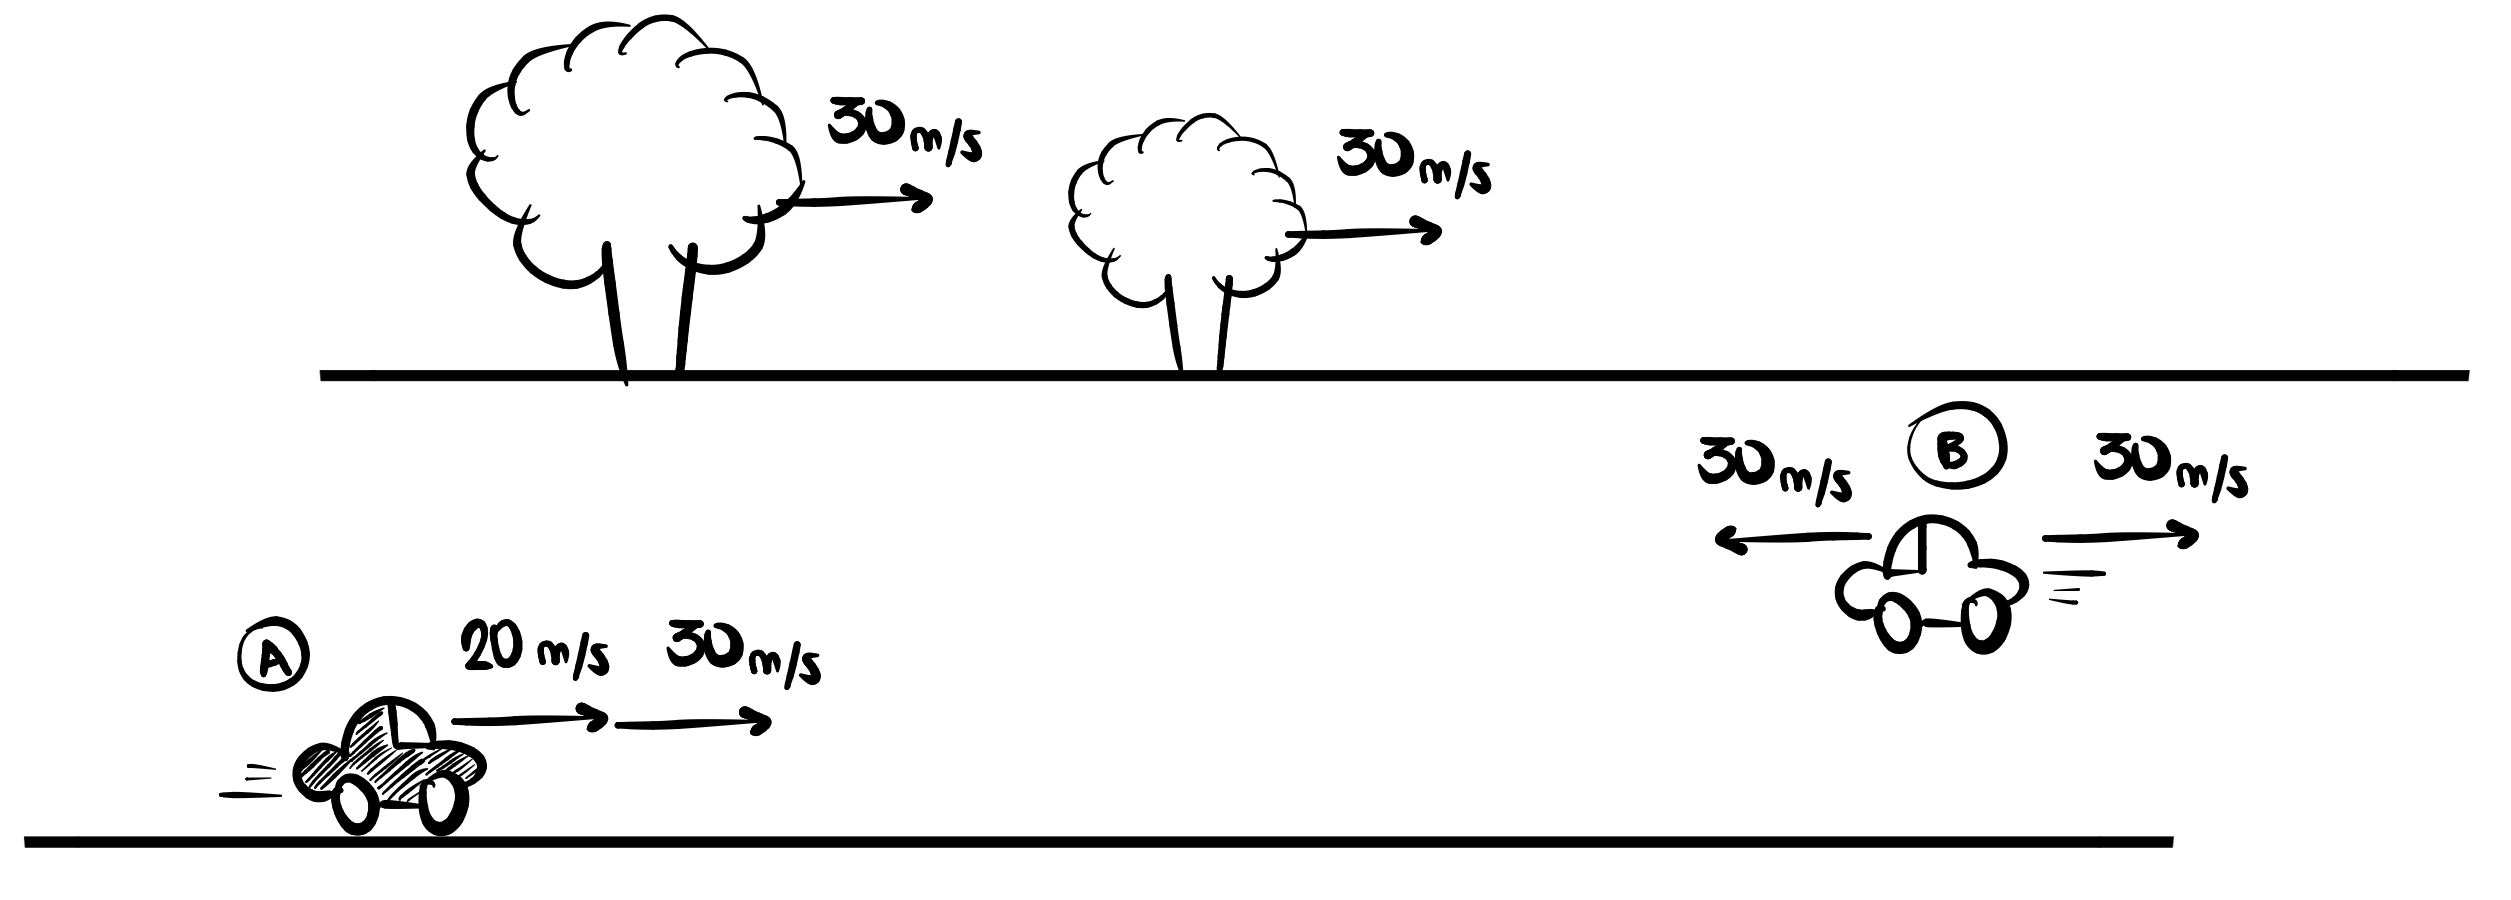
\includegraphics[width=0.6\linewidth]{imagensmecanica/velrelativaemudancaderefAB2.jpeg}
\captionof{figure}{Fazendo a mudança de referencial terra $\to$ B.}
\label{velrelativaemudancaderefAB2}
} 

Note que, ao sobrepor as velocidades, a velocidade do carro $B$ – 30 m/s para a direita sobreposta com 30 m/s para a esquerda – se anulará, que é justamente o que queríamos e o motivo de termos feito tal operação: estamos, agora, no referencial de Bohr. Este é o referencial no qual Bohr está parado. A Figura \ref{velrelativaemudancaderefAB3} mostra as velocidades finais dos corpos neste referencial: a velocidade de $A$ será de $20+30=50$ m/s e as velocidades das árvores serão de $30$ m/s para a direita.

{
\centering
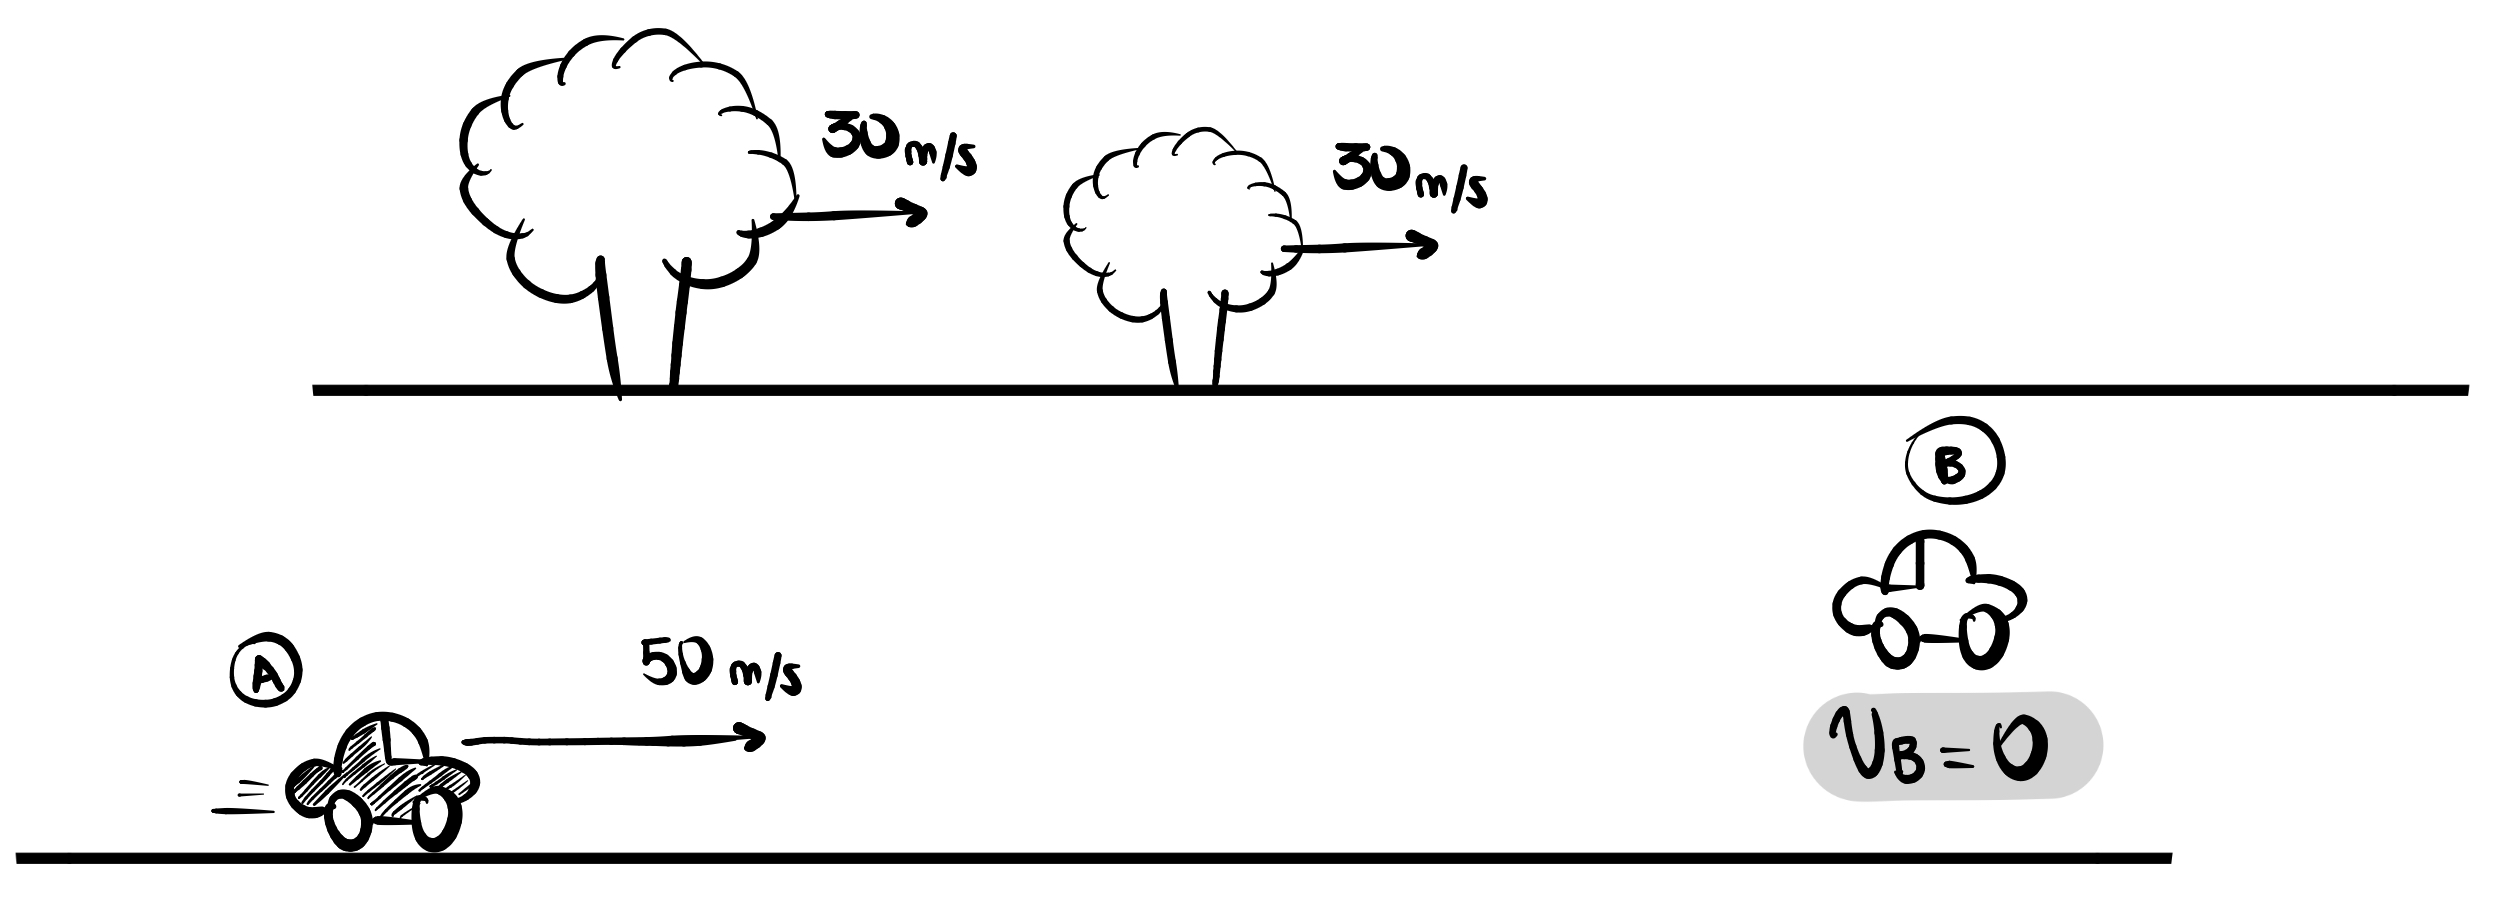
\includegraphics[width=0.6\linewidth]{imagensmecanica/velrelativaemudancaderefAB3.jpeg}
\captionof{figure}{Velocidades no referencial de $B.$}
\label{velrelativaemudancaderefAB3}
} 
\vspace{0.3cm}

O conceito de velocidade de uma árvore pode parecer um pouco estranho, mas vamos ler e comparar as situações físicas. Neste momento, é bem importante que o leitor observe e compare a Figura \ref{velrelativaemudancaderefAB1}, que mostra o problema no referencial das árvores, com a Figura \ref{velrelativaemudancaderefAB3}, que mostra o problema no referencial de $B.$ Note que, no referencial das árvores, elas estão paradas e o carro $B$ se aproxima delas a uma taxa de $30$ m/s a cada segundo. Já no referencial do carro $B$ é ele quem está parado e são as árvores que passam por ele a $30$ m/s. Razoável, não? Quando vocês está de carro, em uma estrada, não é essa a percepção que você tem -- de que as árvores estão passando por você e ficando para trás a uma alta velocidade?

Pois bem. Note que a física é a mesma, só muda a perspectiva: no referencial da árvore ela está parada e o carro passa por ela; no referencial do carro ele está parado e as árvores passam por ele. Tudo na mesma taxa de $30$ m/s, naturalmente -- a física não foi modificada, só estamos mudando de perspectiva.

Note, na Figura \ref{velrelativaemudancaderefAB1}, no referencial das árvores, que a cada segundo que passa o carro $A$ se aproxima 20 metros de $B$, e o carro $B$, que também se move em direção a $A$, se aproxima deste, portanto, de $30$ metros neste mesmo segundo. Ou seja, podemos dizer que, a cada segundo, a distância entre os carros $A$ e $B$ diminui de 50 metros. Essa é a leitura no referencial das árvores. Já observando a Figura \ref{velrelativaemudancaderefAB3}, notamos que o carro $B$ se encontra parado e o carro $A$ se aproxima dele a $50$ m/s: de novo, trata-se da mesma física, apenas vista por uma perspectiva diferente. Tal figura mostra todas as velocidades no referencial de $B.$

Vimos, neste caso, que sendo $v_A=20$ m/s a velocidade de $A$ em relação à terra e $v_B=30$ m/s a velocidade de $B$ em relação à terra, ao fazermos a mudança de referencial, obtivemos que a velocidade $v_{AB}$ do carro $A$ em relação ao carro $B$ era dada por

$$ \boxed{v_{AB}=v_A+v_B = 20+30=50 \text{ m/s.}}$$

Em resumo, para obtermos a velocidade de $A$ em relação a um referencial $B$, ou seja, para operarmos uma mudança de referencial, dois pontos merecem ser destacados, haja vista que todo o processo se sustenta neles:

\begin{enumerate}
    \item [(i)] Resolver o problema no referencial de $B$ é resolver o problema no qual $B$ está parado.

    \item [(ii)] A fim de parar um certo corpo, digamos $B,$ adiciona-se o oposto de sua velocidade a todos os corpos do sistema. Após efetuar a sobreposição de velocidades, a velocidade de $B$ será zero -- que é o que queríamos fazer -- de modo que estaremos no referencial de $B$: teremos, agora, as velocidades dos demais corpos no referencial de $B.$
\end{enumerate}


Poderíamos, por exemplo, a partir da situação da Figura \ref{velrelativaemudancaderefAB1}, escolher parar o carro $A$ para observar o problema na perspectiva de Aristóteles. Lembre-se que o referencial de Aristóteles é o referencial no qual ele está parado, por isso buscaremos zerar a velocidade de $A.$ Para isso, como ele se move a $20$ m/s para a direita, adicionaremos a velocidade de $20$ m/s para a esquerda a todas as partículas do sistema, como mostra a Figura \ref{velrelativaemudancaderefAB5}. Perceba que a velocidade de Aristóteles agora será, naturalmente, nula. A velocidade de $B$ em relação a $A$ será dada pela sobreposição das duas velocidades, ou seja $20+30=50$ m/s.

\vspace{0.3cm}
{
\centering
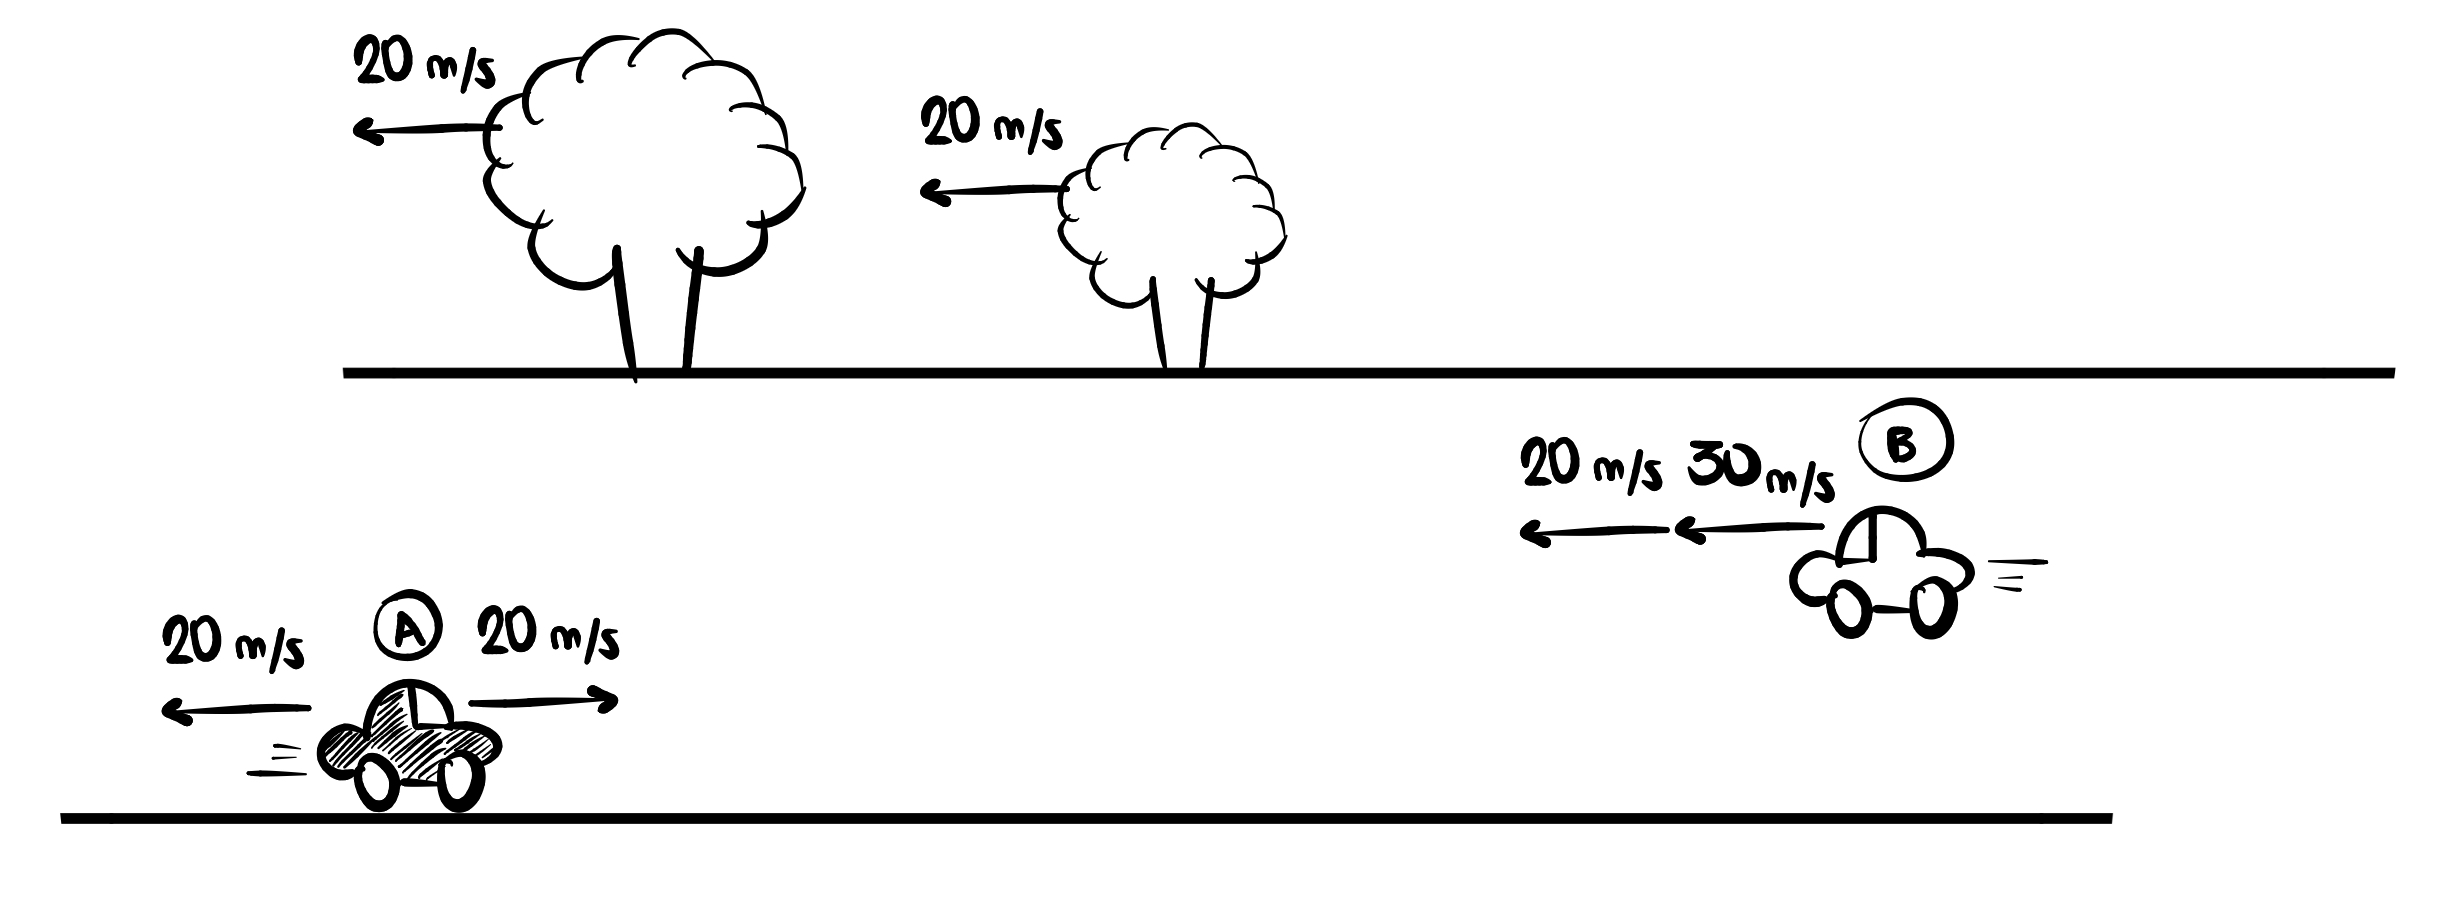
\includegraphics[width=0.6\linewidth]{imagensmecanica/velrelativaemudancaderefAB5.jpeg}
\captionof{figure}{Fazendo a mudança de referencial terra $\to$ A.}
\label{velrelativaemudancaderefAB5}
} 
\vspace{0.3cm}

Por fim, a Figura \ref{velrelativaemudancaderefAB4} mostra a situação final no referencial de $A.$ Perceba que nossa leitura é bem parecida: no referencial da terra as árvores estão paradas e o carro $A$ passa por elas a uma velocidade de $20$ m/s; já no referencial de $A$ é ele quem está parado e as árvores passam por ele a uma velocidade de $20$ m/s.

No referencial das árvores (terra) a distância entre $A$ e $B,$ como analisamos anteriormente, encurtava de $50$ metros a cada segundo; já no referencial de $A$ vemos que ele está parado enquanto $B$ se aproxima dele a $50$ metros por segundo -- a mesma Física, apenas vista por perspectivas diferentes.

{
\centering
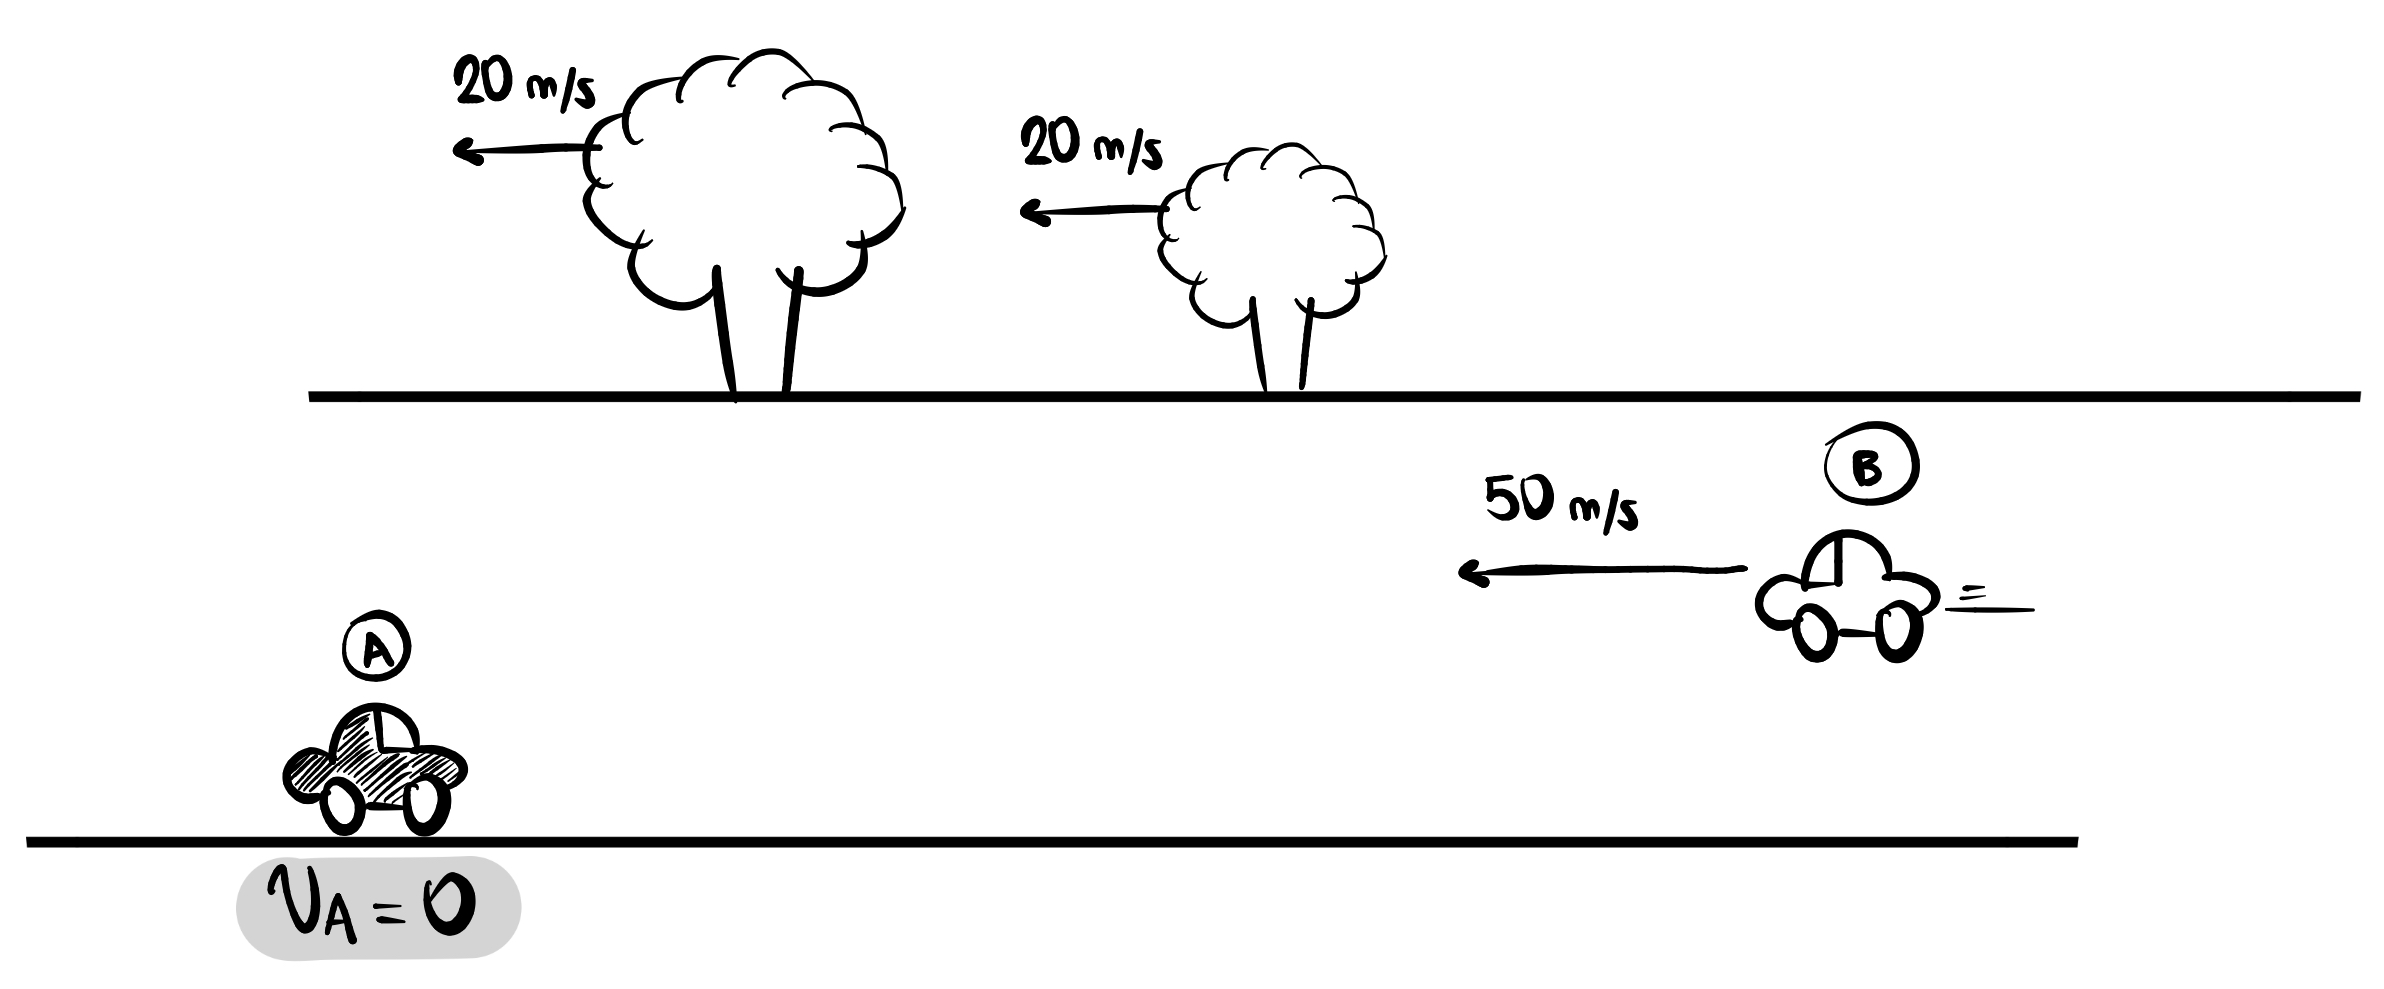
\includegraphics[width=0.6\linewidth]{imagensmecanica/velrelativaemudancaderefAB4.jpeg}
\captionof{figure}{Velocidades no referencial de $A.$}
\label{velrelativaemudancaderefAB4}
}    
\vspace{0.3cm}
Sugiro que o leitor tente mudar para o referencial de $A$, como exercício, a partir da situação da Figura \ref{velrelativaemudancaderefAB3}, isto é, do referencial de $B.$ \footnote{Dica: para fazer isso basta perceber que, para anular a velocidade de $A,$ é necessário adicionar uma velocidade de $50$ m/s para a esquerda em todos os corpos do sistema.} Após fazê-lo, observe a simetria entre $A$ e $B$ pelas Figuras \ref{velrelativaemudancaderefAB3} e  \ref{velrelativaemudancaderefAB4}: no referencial de $B$ ele está parado, e $A$ se aproxima dele a $50$ m/s. Já no referencial de $A$ é ele quem está parado, e $B$ se aproxima dele a $50$ m/s -- perceba, mais uma vez, como a física concorda. São apenas leituras de referenciais distintos. Ou seja, estamos aqui concluindo que

$$ v_{AB} = v_{BA},$$

\noindent ou seja, a velocidade $v_{AB}$ de $A$ em relação a $B$ é exatamente a mesma, em valor absoluto, que a velocidade $v_{BA}$ de $B$ em relação a $A$ -- as duas foram obtidas somando os valores $v_A$ e $v_B$ das velocidades de $A$ e $B$ em relação às árvores.

O leitor poderia, como exercício, considerar um contexto como o da Figura \ref{velrelativaemudancaderefAB1}, porém com $B$ se movendo para a direita, no mesmo sentido de $A.$ Fazendo a mudança de referencial da terra para o referencial de $A$ ou de $B$, será possível obter a velocidade $v_{AB}$ de $A$ em relação a $B$ (ou a velocidade $v_{BA}$ de $B$ em relação a $A,$ mas já sabemos que essas duas coisas são iguais), de modo que será possível compreender de onde vem o sinal negativo na Equação \eqref{mecanica_eq_velocidaderelativa}.

Por fim, para obtermos de forma geral a Equação \eqref{mecanica_eq_velocidaderelativa}, convido o leitor a observar a Figura \ref{vrelsentidooposto}. Não vou me delongar aqui e deixarei o leitor observar a figura e pensar por si só -- note apenas que, na primeira imagem temos a situação no referencial das árvores, na imagem central temos a operação da mudança de referencial e na última imagem temos a situação no referencial de $B.$

{
\centering
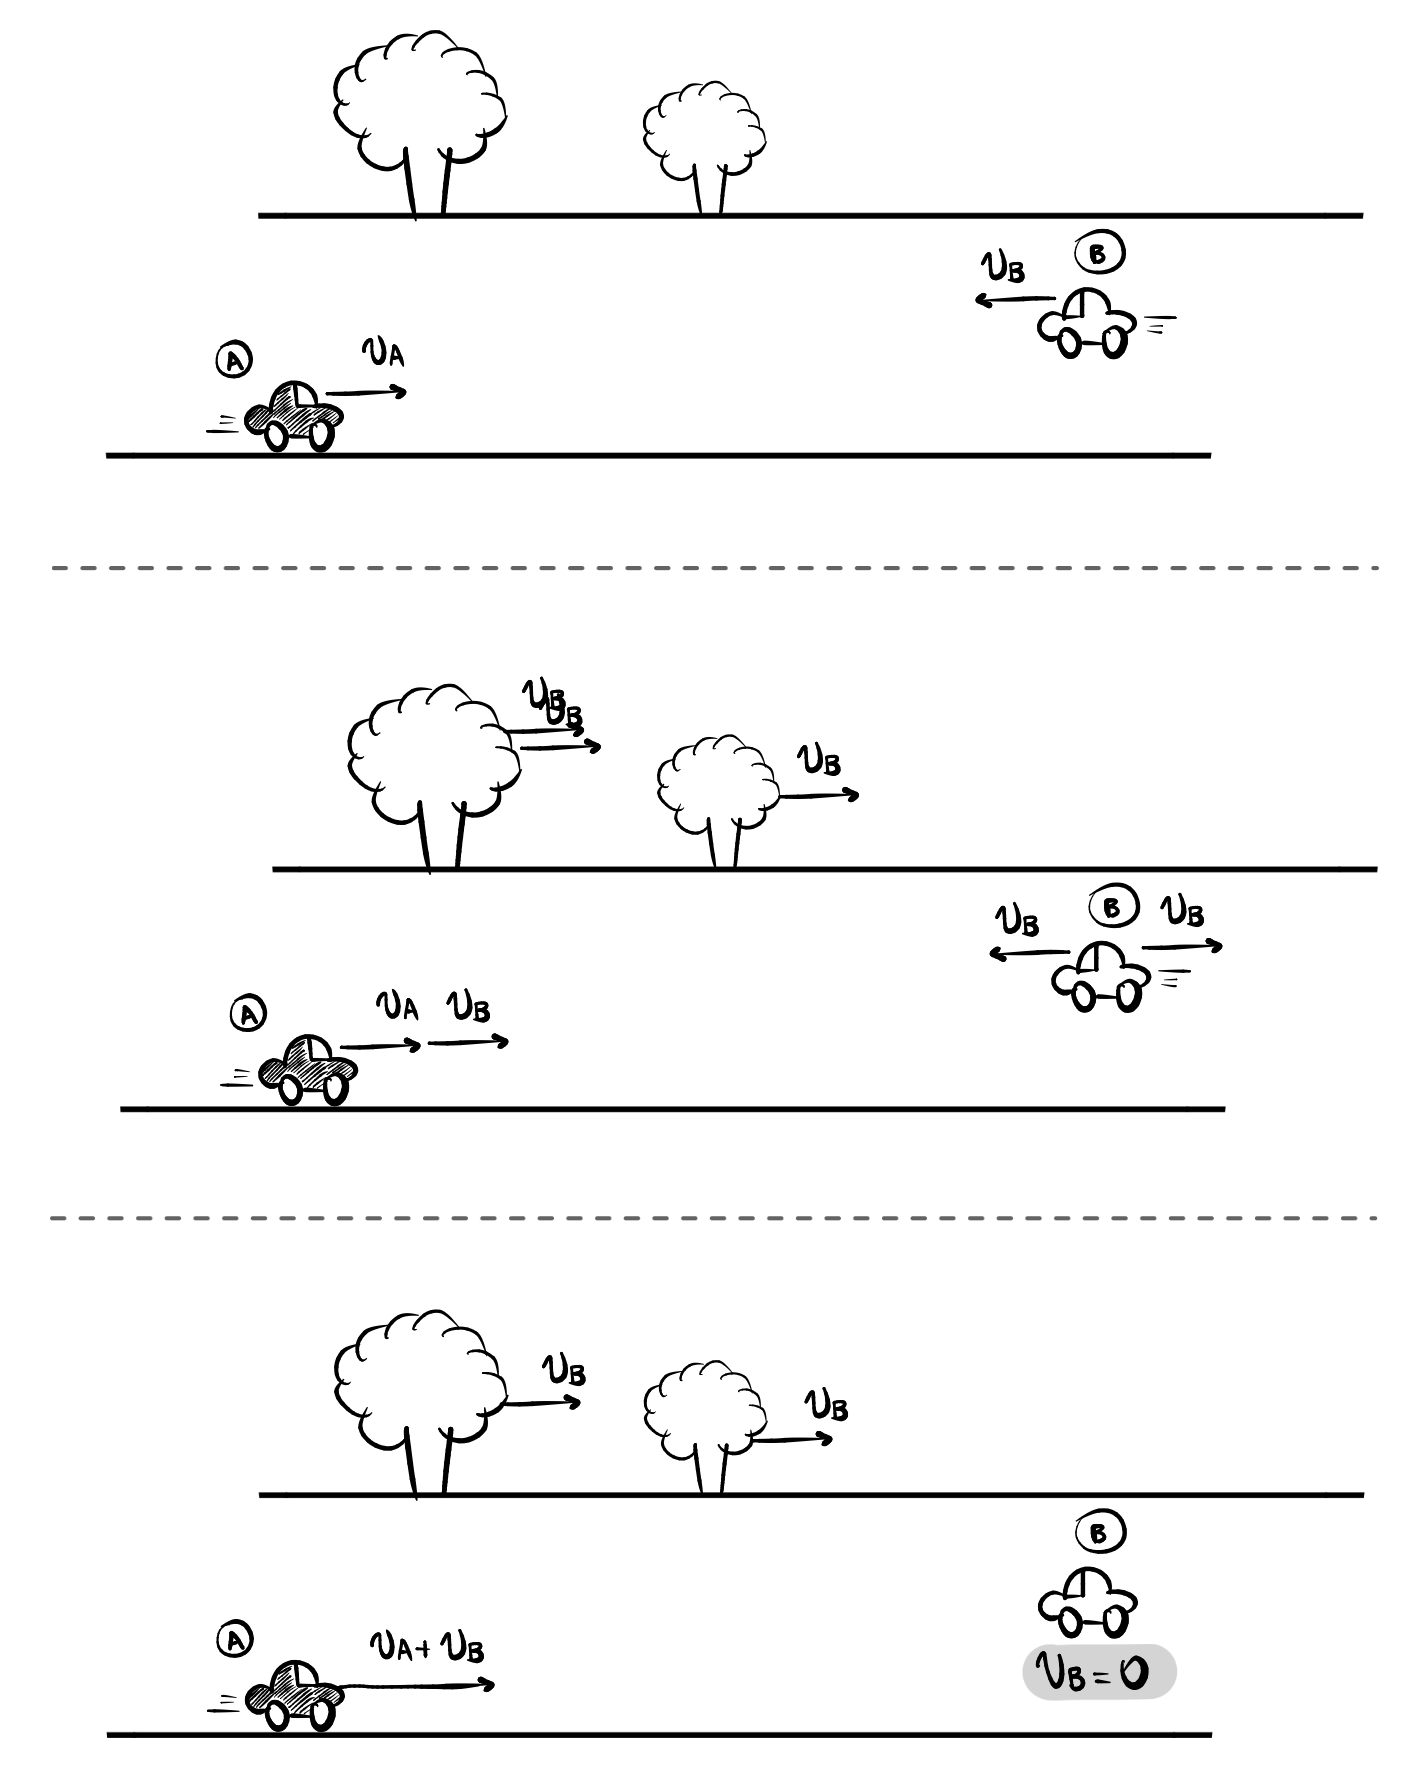
\includegraphics[width=0.6\linewidth]{imagensmecanica/vrelsentidooposto.png}
\captionof{figure}{Obtenção da velocidade relativa $v_{AB}$ de $A$ em relação a $B$ quando os dois corpos se movem na mesma direção mas em sentido contrários.}
\label{vrelsentidooposto}
}    
\vspace{0.3cm}
A partir de tal figura, o leitor concluirá que, sempre que dois carros se moverem na mesma direção mas em sentidos opostos, a velocidade de um em relação ao outro (ou do outro em relação ao um -- o que dá na mesma) será dada pela soma das suas velocidades, isto é, se $v_A$ e $v_B$ são as velocidades de $A$ e $B$ em relação à estrada, então a velocidade de $A$ em relação $B$ será dada por

$$ \boxed{v_{AB}=v_A+v_B.}$$

Já a Figura \ref{vrelsentidoigual} mostra a mesma situação, porém para os corpos que se movem no mesmo sentido -- a primeira imagem mostra a situação no referencial das árvores, na imagem central temos a operação da mudança de referencial e na última imagem temos a situação no referencial de $B.$


{
\centering
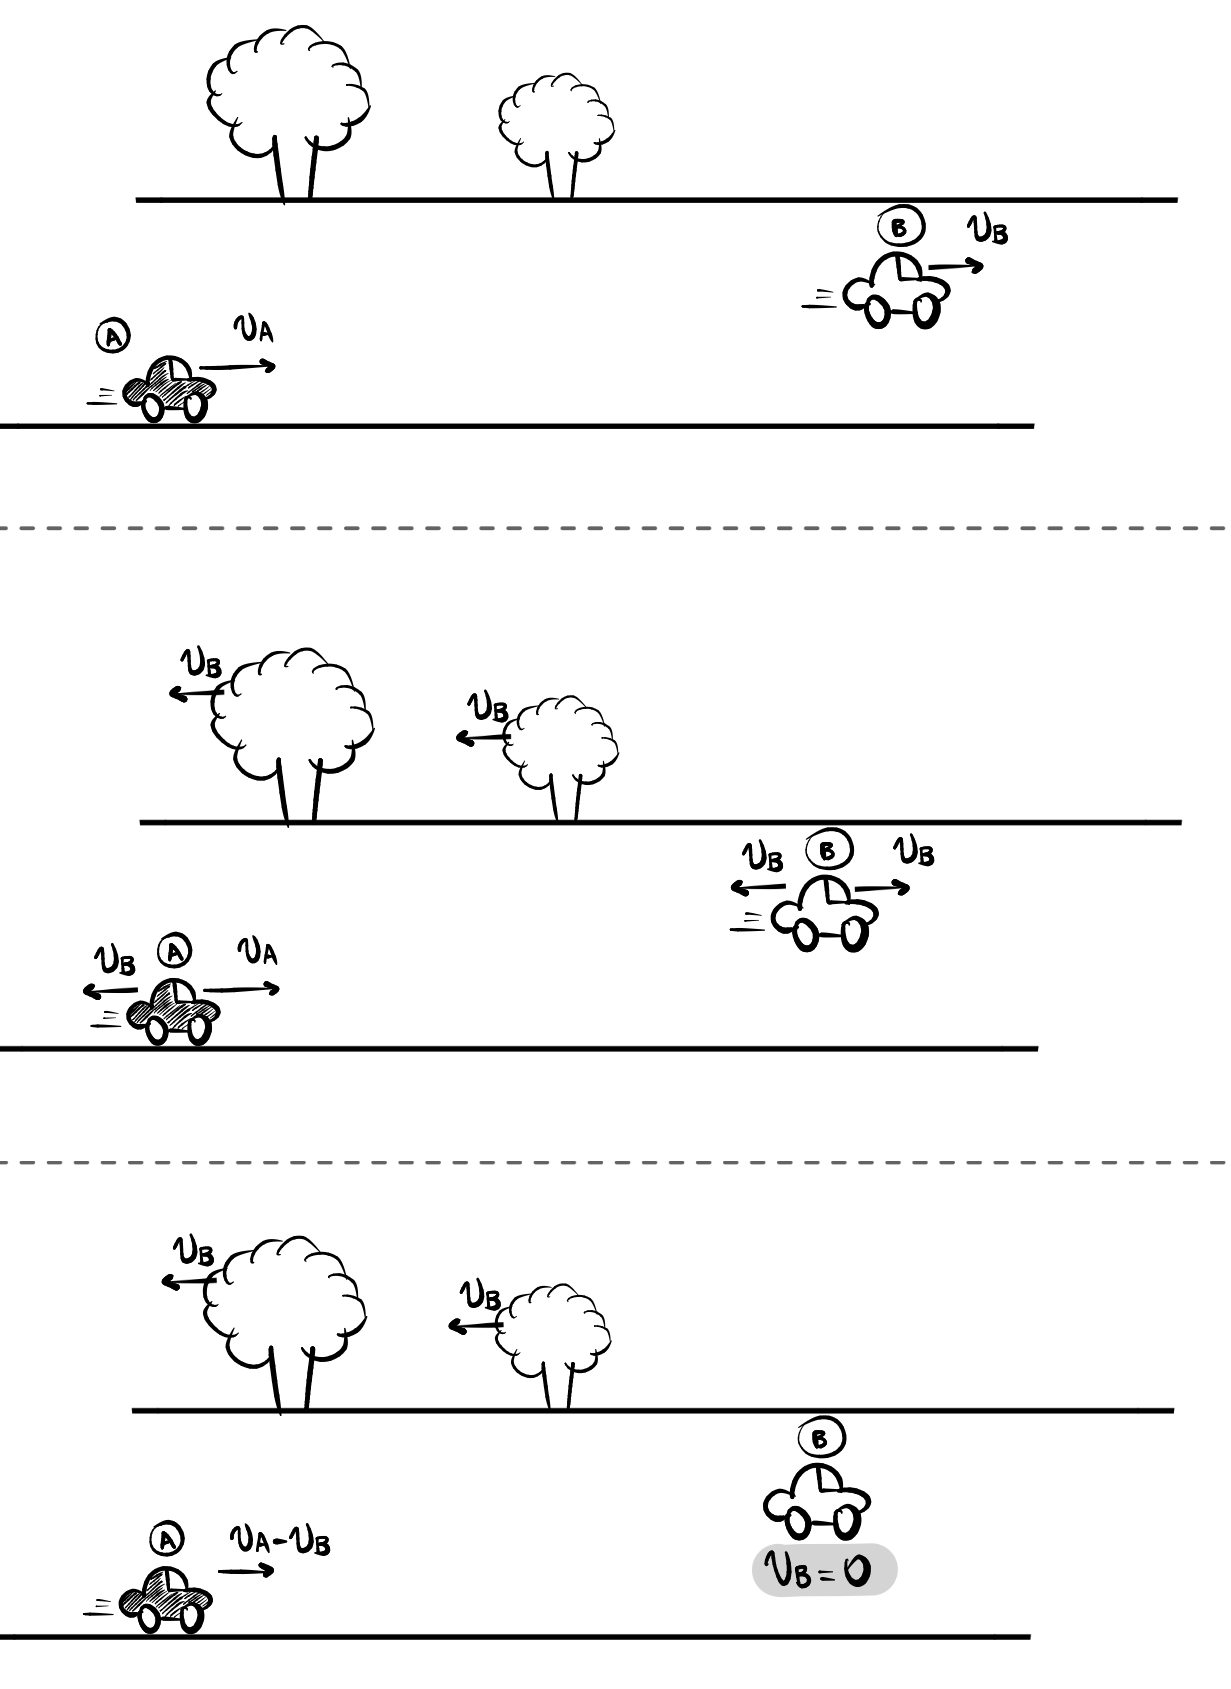
\includegraphics[width=0.5\linewidth]{imagensmecanica/vrelsentidoigual.jpeg}
\captionof{figure}{Obtenção da velocidade relativa $v_{AB}$ de $A$ em relação a $B$ quando os dois corpos se movem na mesma direção e mesmo sentido.}
\label{vrelsentidoigual}
}    
\vspace{0.3cm}
Dessa análise, o leitor concluirá que, sempre que dois carros se moverem na mesma direção e mesmo sentido, a velocidade de um em relação ao outro será dada pela diferença de suas velocidades, isto é, se $v_A$ e $v_B$ são as velocidades de $A$ e $B$ em relação à estrada, então a velocidade de $A$ em relação $B$ será dada por

$$ \boxed{v_{AB}=v_A-v_B.}$$

A Equação \eqref{mecanica_eq_velocidaderelativa} sintetiza as duas conclusões acima tiradas. Espero que, com toda essa discussão aqui feita, o leitor não se contente em apenas memorizar tal equação, mas compreenda, com profundidade, a sua natureza -- a operação de mudança de referencial.

\secgfe{Onde é usada}

Como dito anteriormente: toda velocidade é relativa. Qualquer velocidade dada sempre é em relação a algum sistema de referência específico; logo, o conceito de velocidade relativa é usado basicamente em qualquer contexto em que se fale de velocidade. Contudo, usar diretamente a Equação \eqref{mecanica_eq_velocidaderelativa} é um recurso do qual lançaremos mão quando quisermos observar o problema na perspectiva de outro referencial. Em muitos contextos, como veremos nos exemplos, fazer uma mudança de referencial simplifica drasticamente a matemática para resolver o exercício.


\secgfe{Erros comuns}

O erro mais comum aqui é o estudante se ater a memorizar a Equação \eqref{mecanica_eq_velocidaderelativa} sem entender o que de fato está por trás dela: uma mudança de referencial. Para o estudante que entendeu em detalhes o desenvolvimento feito na seção anterior, não só ficará totalmente dispensável memorizar a equação em questão, como ele terá muito mais profundidade e domínio acerca do que está fazendo quando usar o conceito de velocidade relativa.


\secgfe{Observações}

O conceito que construímos aqui é muito mais amplo do que o contexto no qual o aplicamos. A ideia de que estudar o problema no referencial $X$ é avaliar o problema na perspectiva na qual $X$ está parado -- e, portanto, para pará-lo, basta adicionar o oposto da sua velocidade à todas as partículas do sistema -- é um conceito que valerá para movimentos bidimensionais ou mesmo tridimensionais. É claro que, em tais movimentos, como estudaremos na Cinemática Vetorial, o tratamento geométrico para operar uma mudança de referencial pode ser um pouco mais complicado, mas, ainda assim, o princípio será exatamente o mesmo.

Sendo assim, cabe a observação de que o princípio que aqui construímos é geral: \textbf{avaliar um problema físico no referencial de $A$ é estudar o problema no referencial no qual $A$ está parado. Para pará-lo, basta adicionar o oposto de sua velocidade à todas as partículas envolvidas no sistema.}


\vspace{0.3cm}


\begin{exemplo}[Nível I]\label{exemplo_cinematica_vrelativa01}

Dois carros, separados de $600$m um do outro, se movem um em direção ao outro. Se as suas velocidades são de $20$ m/s e $40$ m/s, após quanto tempo eles se encontram?


\resolucao


Esse é o problema mais clássico de toda a Cinemática e, com o desenvolver dos nossos estudos, veremos diferentes forma de resolvê-lo ao longo das próximas seções.\\

Perceba que o enunciado nos forneceu velocidades mas sequer disse em relação a quem elas são medidas. Como já conversamos, isso acaba sendo comum e, quando ocorre, devemos partir da premissa de que tais velocidades são em relação à terra -- em relação a um indivíduo parado, na estrada. \\

Em geral é sempre mais complicado resolver um problema como este se os dois carros estão se movendo. Desse modo, façamos uma mudança de referencial para parar um dos carros e tentar simplificar o problema. Seja $A$ o carro cuja velocidade é de $20$ m/s e $B$ o carro cuja velocidade é de $40$ m/s. A Figura \ref{fig_mec_mudancareferencialexemplo01} mostra a mudança de referencial para o carro $B:$ adicionamos uma velocidade de $40$ m/s para a direita em todas as partículas do sistema, de modo que a velocidade resultante de $B$ é zero -- estamos, portanto, no referencial do carro B -- e a velocidade resultante de $A$ é de $60$ m/s, como mostra última imagem da figura.

{
\centering
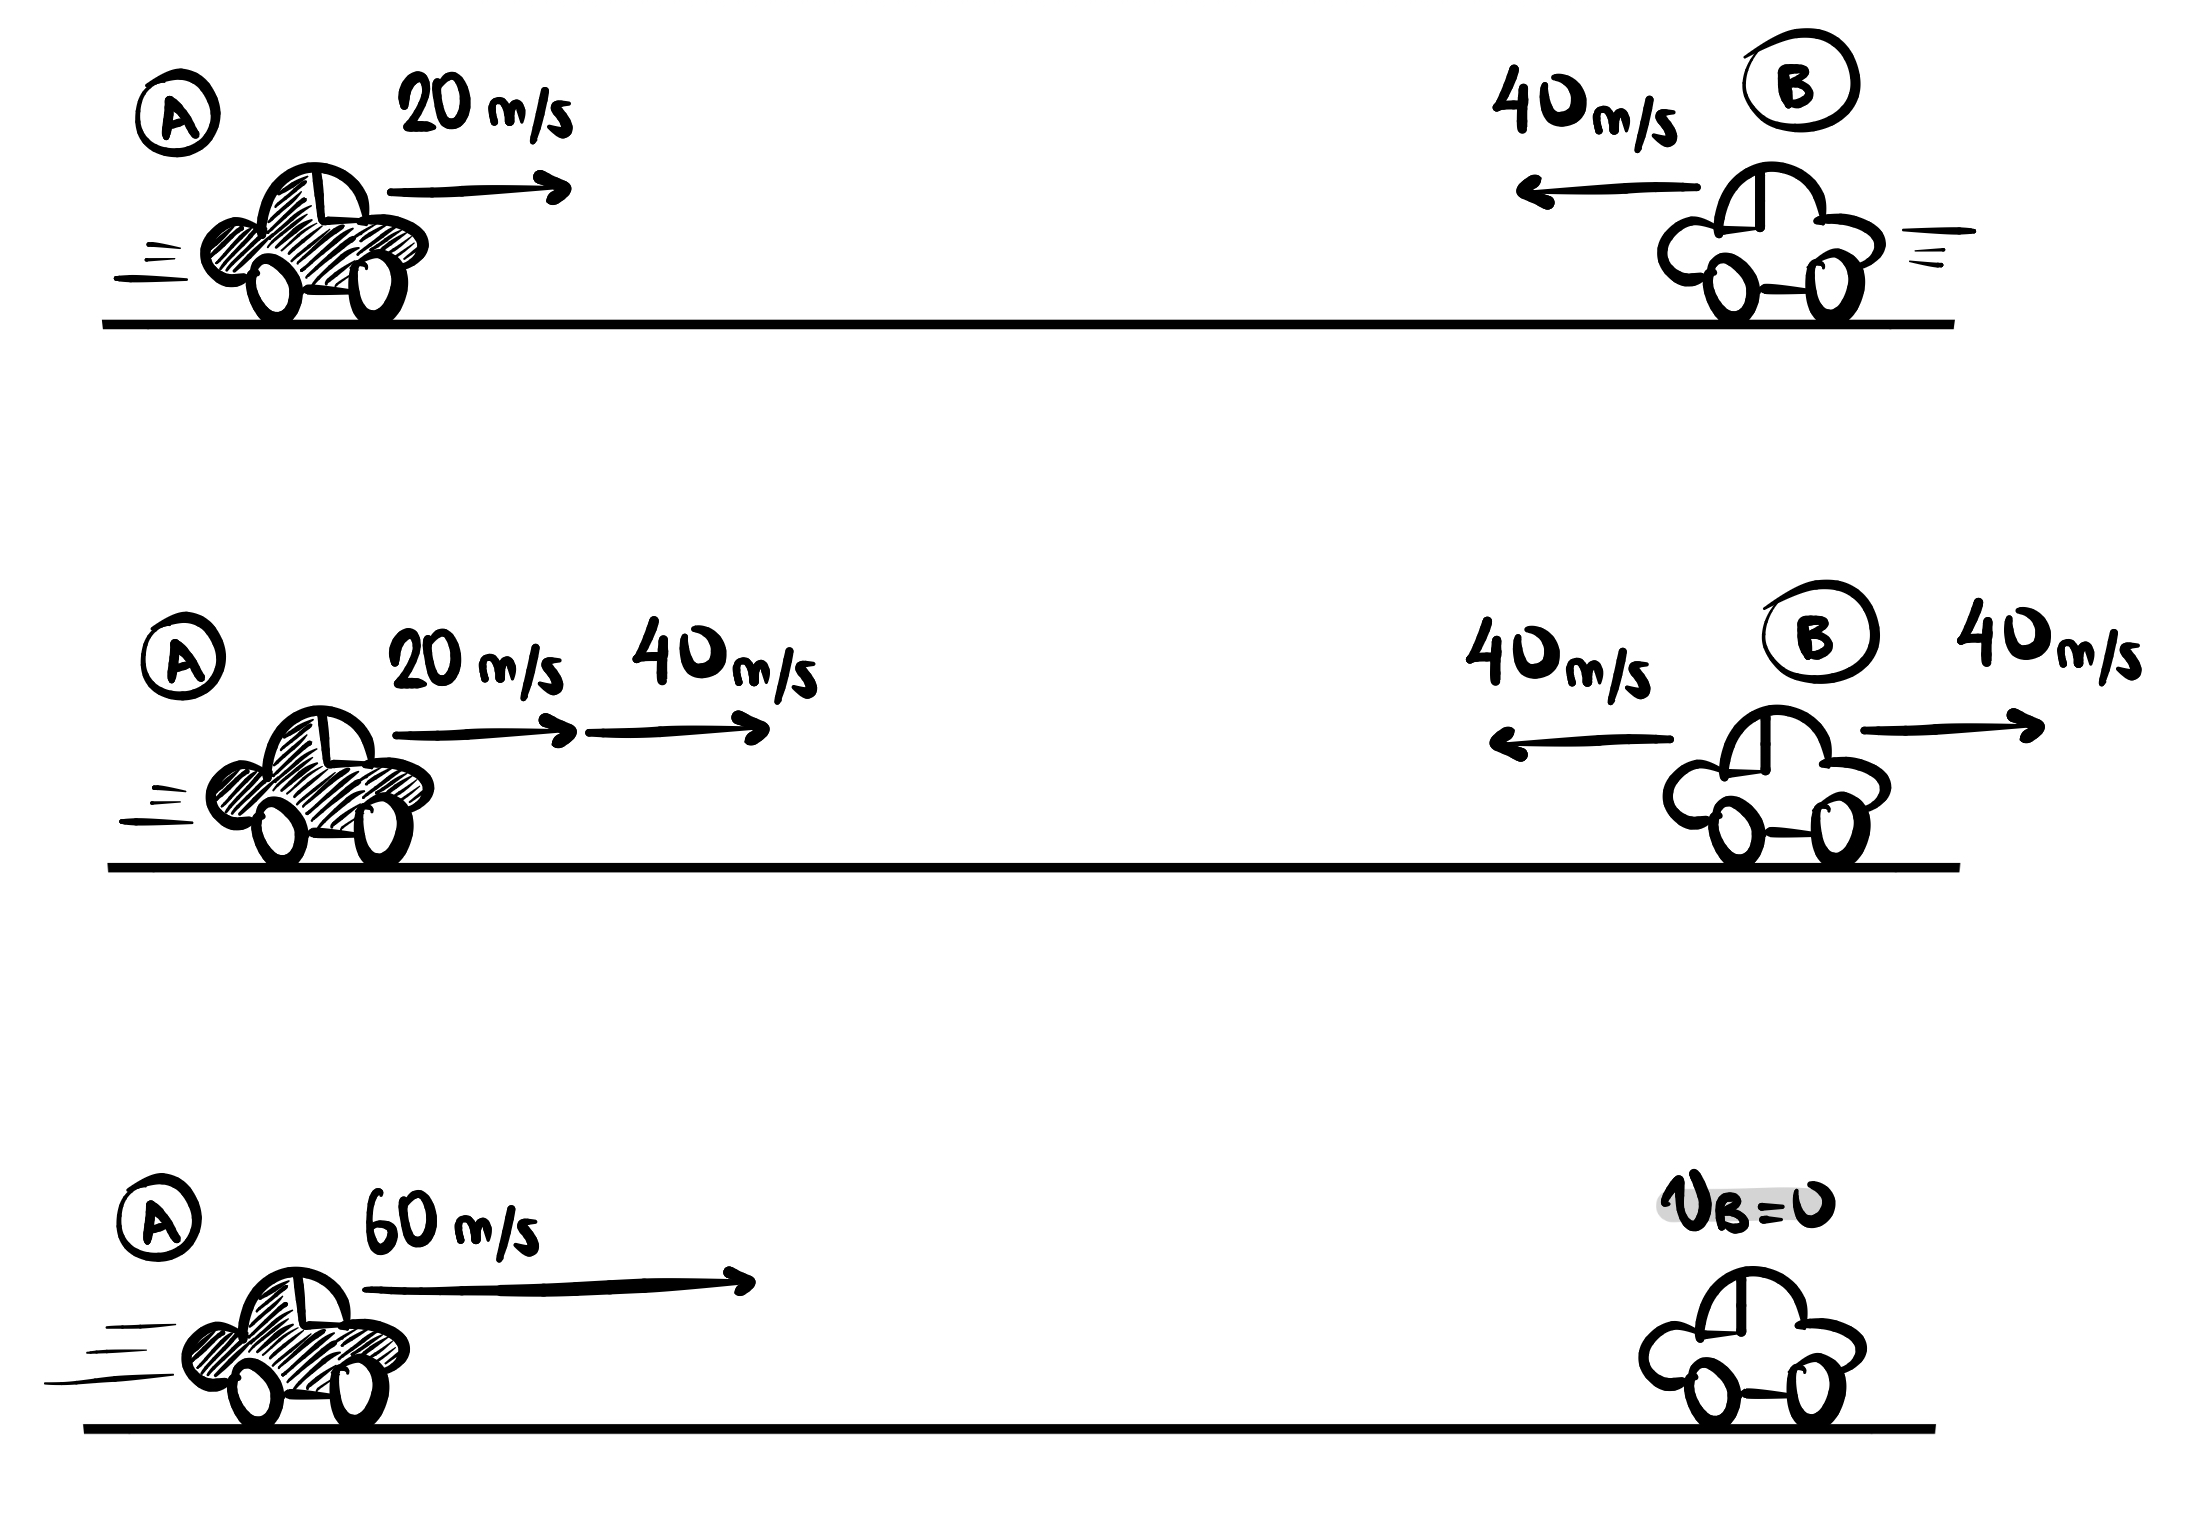
\includegraphics[width=0.5\linewidth]{imagensmecanica/mudancareferencialexemplo01.jpeg}
\captionof{figure}{Mudando do referencial da Terra para o referencial do carro B -- referencial no qual B está parado.}
\label{fig_mec_mudancareferencialexemplo01}
} 
\vspace{0.3cm}

Perceba como o problema agora se tornou mais fácil: temos dois carros, afastados um do outro de 600m. Um deles está parado, e o outro se aproxima dele a uma velocidade de $60$ m/s. O problema ficou tão simples que não é preciso muito mais conhecimento para perceber que, avançando $60$ metros a cada segundo, levar-se-á $10$ segundos para varrer os 600 metros que distanciam os dois carros. Logo, em $10$ segundos os carros terão se encontrado.

Como é a primeira vez que isso foi feito, cabe destacarmos alguns pontos importantes:

\begin{enumerate}
    \item [(i)] Alguém poderia pensar: \textit{``computamos que leva 10s para os carros se encontrarem, mas isso foi no referencial do carro $B.$ O que me garante que o tempo será o mesmo no referencial original, da terra?''}

    Seria uma boa pergunta -- e retornaremos a ela no futuro. Por hora, eu deixo ao leitor apenas a provocação: digamos que você e um amigo disparem um cronômetro em seus respectivos relógios, um ao lado do outro, no mesmo instante. Digamos que isso ocorre às 08 horas da manhã. Daí você pega um ônibus e vai à escola e, no fim do dia, digamos às 17 horas, retorna à casa de seu amigo. Ao comparar os tempos marcados nos cronômetros, em qual relógio terá passado mais tempo?

    Pois bem...se passaram-se 9 horas, isso parece ser algo absoluto, não? Algo que não depende do relógio que usamos para marcar, ou de qual referencial marcou a passagem do tempo...concorda?\footnote{Conheci um cara que discordava disso. Seu nome era Albert Einstein, mas isso é prosa para o outro volume da coleção...}

    \item [(ii)] Como já levantamos, essa não é a única forma de resolver o problema. Existem pelo menos outras duas ou três que veremos quando construirmos novas equações. Contudo, já adianto ao leitor, essa é a forma que o autor julga ser a melhor -- é que torna a situação e, consequentemente, os cálculos matemáticos, os mais simples de todos.
\end{enumerate}


\end{exemplo}



\vspace{0.3cm}






\begin{exemplo}[Nível II (UFMG - 2001)]\label{exemplo_cinematica_vrelativa02}

Um menino flutua em uma bóia que está se movimentando, levada pela correnteza de um rio. Uma outra bóia, que flutua no mesmo rio a uma certa distância do menino, também está descendo com a correnteza. A posição das duas bóias e o sentido da correnteza estão indicados na figura.


{
\centering
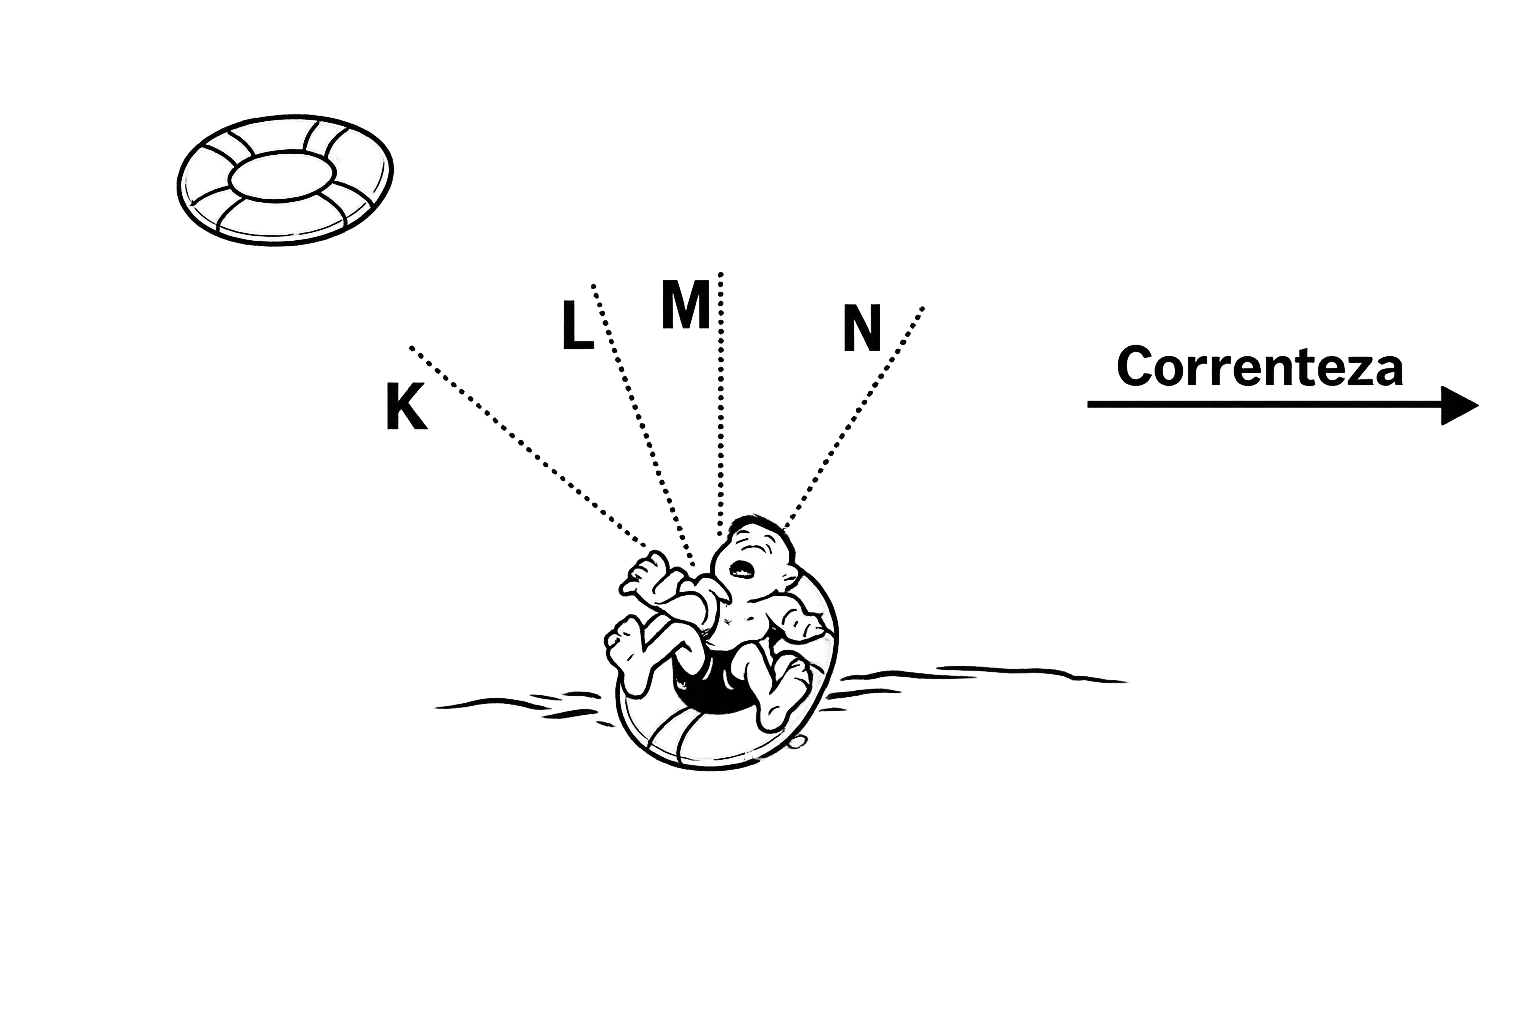
\includegraphics[width=0.50\linewidth]{imagensmecanica/ufmgboiarioexemplotest.png}
\captionof{figure}{}
\label{fig_mec_ufmgboiarioexemplo}
} 



Considere que a velocidade da correnteza é a mesma em todos os pontos do rio. Nesse caso, para alcançar a segunda bóia, o menino deve nadar na direção indicada pela linha:

\begin{enumerate}
  \item [(a)] K.
  \item [(b)] L.
  \item [(c)] M.
  \item [(d)] N.
\end{enumerate}


\resolucao

O problema, no referencial posto, parece ser mais complicado do que de fato é. Por hora, vamos imaginar que não há correnteza alguma -- as águas do rio são calmas e estão em repouso absoluto. Neste contexto, para qual direção o menino deve nadar para buscar a bóia? Parece óbvio que é na direção K -- a direção que liga o menino à bóia --, certo? \\

Pois bem. Agora quero convencer o leitor de que este é exatamente o caso. O enunciado nos diz que a velocidade da correnteza é a mesma em todos os pontos do rio, logo, a água do rio, a bóia e o menino se movem rio abaixo com a mesma velocidade -- a velocidade $v_c$ da correnteza, ou seja, a velocidade da água do rio. Observe agora a Figura \ref{fig_mec_ufmgboiarioexemplo02}, na qual, em sua primeira imagem, temos a ilustração da situação anteriormente citada. Fazendo a mudança de referencial terra $\to$ rio, ou seja, mudando para o referencial no qual a água do rio está parada, adicionaremos o oposto da velocidade $v_c$ da água do rio a todas as partículas do sistema -- o que está ilustrado na figura do meio.

{
\centering
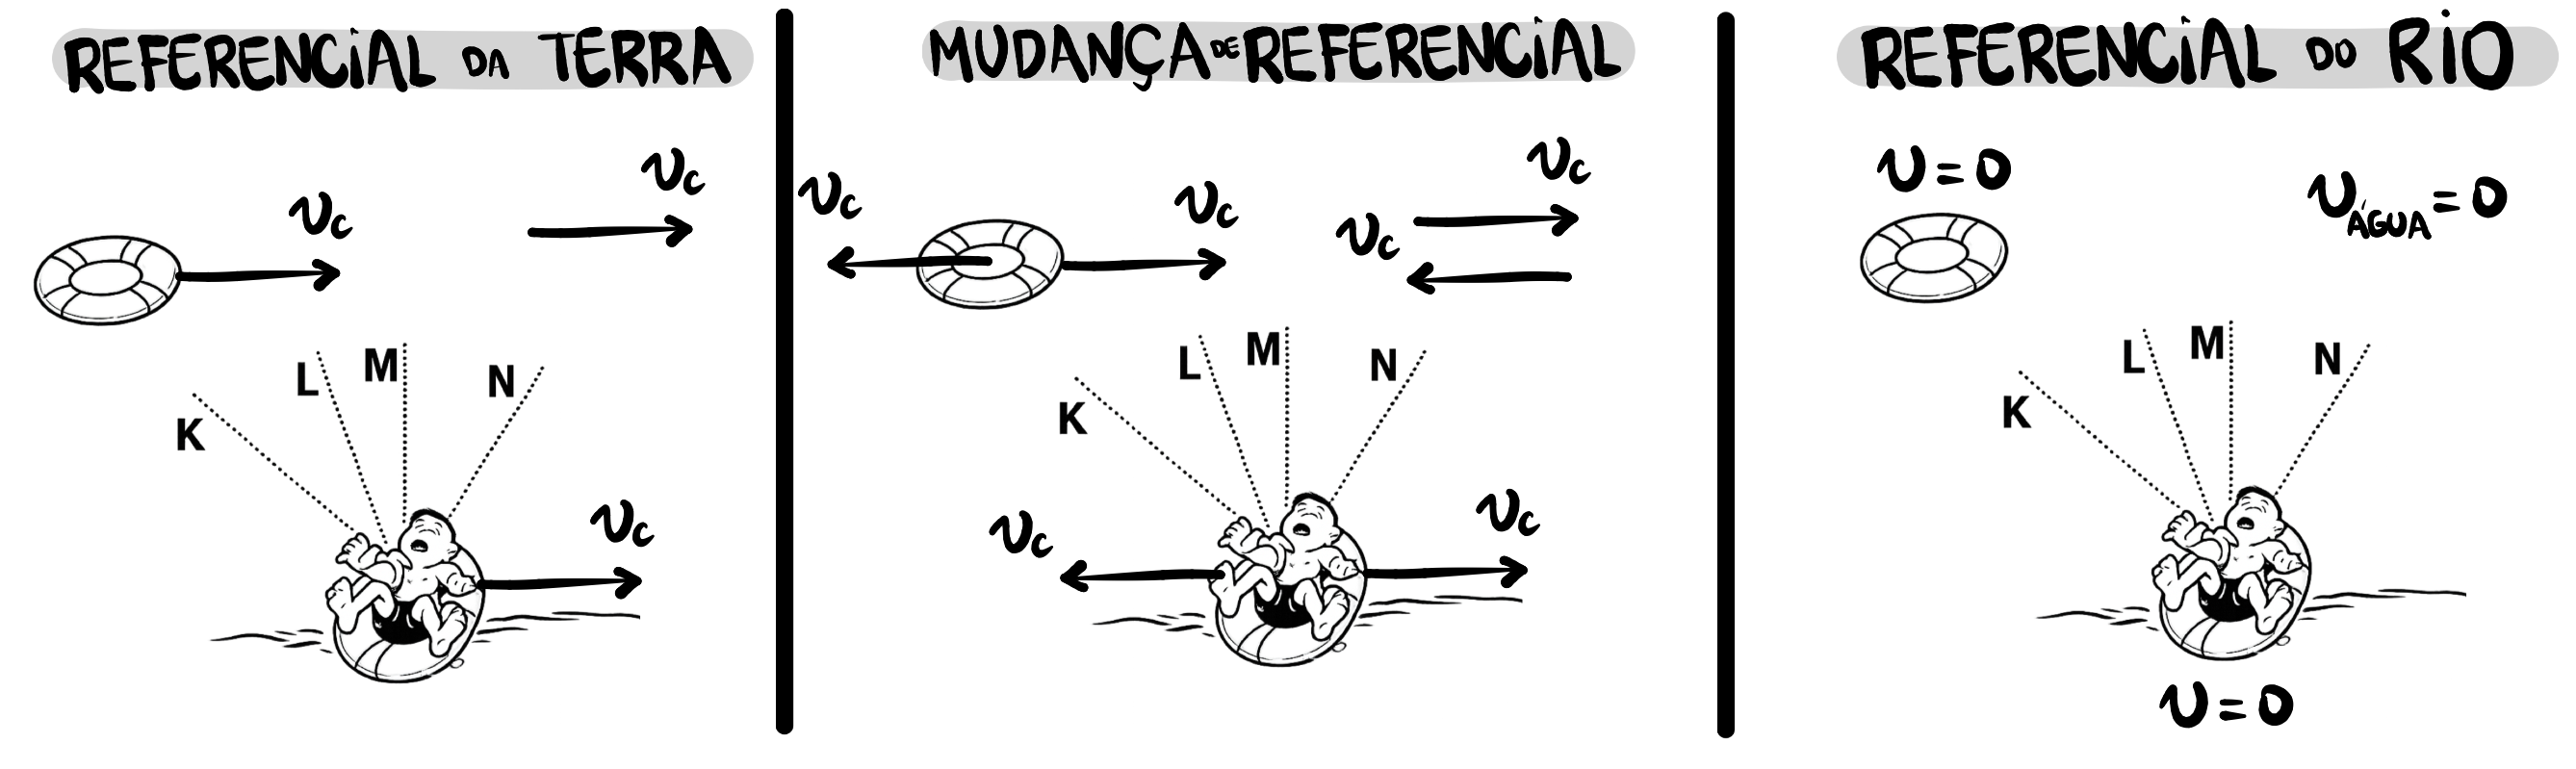
\includegraphics[width=1.0\linewidth]{imagensmecanica/imagem_sem_fundo_2.png}
\captionof{figure}{Mudando do referencial das margens (terra) para o referencial da água (rio).}
\label{fig_mec_ufmgboiarioexemplo02}
} 
\vspace{0.3cm}
A última imagem mostra o resultado: no referencial do rio todos os objetos estão em repouso: a velocidade do menino, da bóia e das águas é nula -- mas este problema já foi resolvido por nós: a direção na qual o menino deve nadar para pegar a bóia é a direção K. \\

Viu só como olhar o problema da perspectiva (referencial) correto muda tudo?


\end{exemplo}



\vspace{0.3cm}






% \begin{exemplo}[Nível III (ITA 2013)]\label{exemplo_cinematica_vrelativa03}

% Ao passar pelo ponto $O$, um helicóptero segue na direção norte com velocidade $v$ constante. Nesse momento, um avião passa pelo ponto $P$, a uma distância $\delta$ de $O$, e voa para o oeste, em direção a $O$, com velocidade $u$ também constante, conforme mostra a figura.

% {
% \centering
% 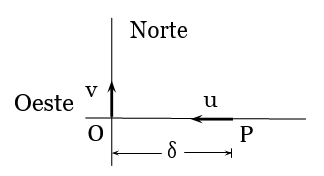
\includegraphics[width=0.3\linewidth]{imagensmecanica/vrelativaITA2013exemplo.png}
% \captionof{figure}{}
% \label{fig_mec_ita2013mudancareferencial}
% } 



% Considerando $t$ o instante em que a distância $d$ entre o helicóptero e o avião for mínima, assinale a alternativa correta.

% \begin{enumerate}
%   \item [(a)] A distância percorrida pelo helicóptero no instante em que o avião
%   alcança o ponto $O$ é $\delta u / v$.
  
%   \item [(b)] A distância do helicóptero ao ponto $O$ no instante $t$ é igual a
%   $\delta u / \sqrt{v^2 + u^2}$.
  
%   \item [(c)] A distância do avião ao ponto $O$ no instante $t$ é igual a
%   $\delta v^2 / (v^2 + u^2)$.
  
%   \item [(d)] O instante $t$ é igual a $\delta v / (v^2 + u^2)$.
  
%   \item [(e)] A distância $d$ é igual a $\delta u / \sqrt{v^2 + u^2}$.
% \end{enumerate}



% \resolucao


% Essa é uma questão cujo nível sobressai neste momento pelo fato de envolver um movimento bidimensional. A sua resolução, desse modo, talvez fique mais clara após o estudo da parte de Cinemática Vetorial. Contudo, a ideia principal é a mudança de referencial, de modo que pareceu oportuno trazê-la neste momento. \\

% Note que o problema é um pouco complicado porque temos dois objetos -- o avião e o helicóptero -- se movendo, e em direções distintas, inclusive. Note que o enunciado não especificou em relação a quem tais velocidades são medidas, de modo que assumimos que tais valores são relativos a um observador parado na terra. Vamos optar, por exemplo, por olhar o problema no referencial do avião -- isto é, o referencial no qual o avião está parado.  \\

% Desse modo, para pará-lo e fazer a mudança de referencial Terra $\to$ Avião, adicionamos a velocidade $u$ para direita a todos os corpos do sistema, como mostra a primeira imagem da Figura \ref{fig_mec_mudancareferencialITA2d}. Isso fará com que o avião esteja parado -- é o que queríamos -- e que a velocidade resultante do helicóptero, neste referencial, seja dada pela soma vetorial das velocidades $v$ e $u$, o que aparece na segunda imagem da figura. Tal velocidade pode ser obtido pelo Teorema de Pitágoras, sendo dado por $w=\sqrt{v^2+u^2.}$

% {
% \centering
% 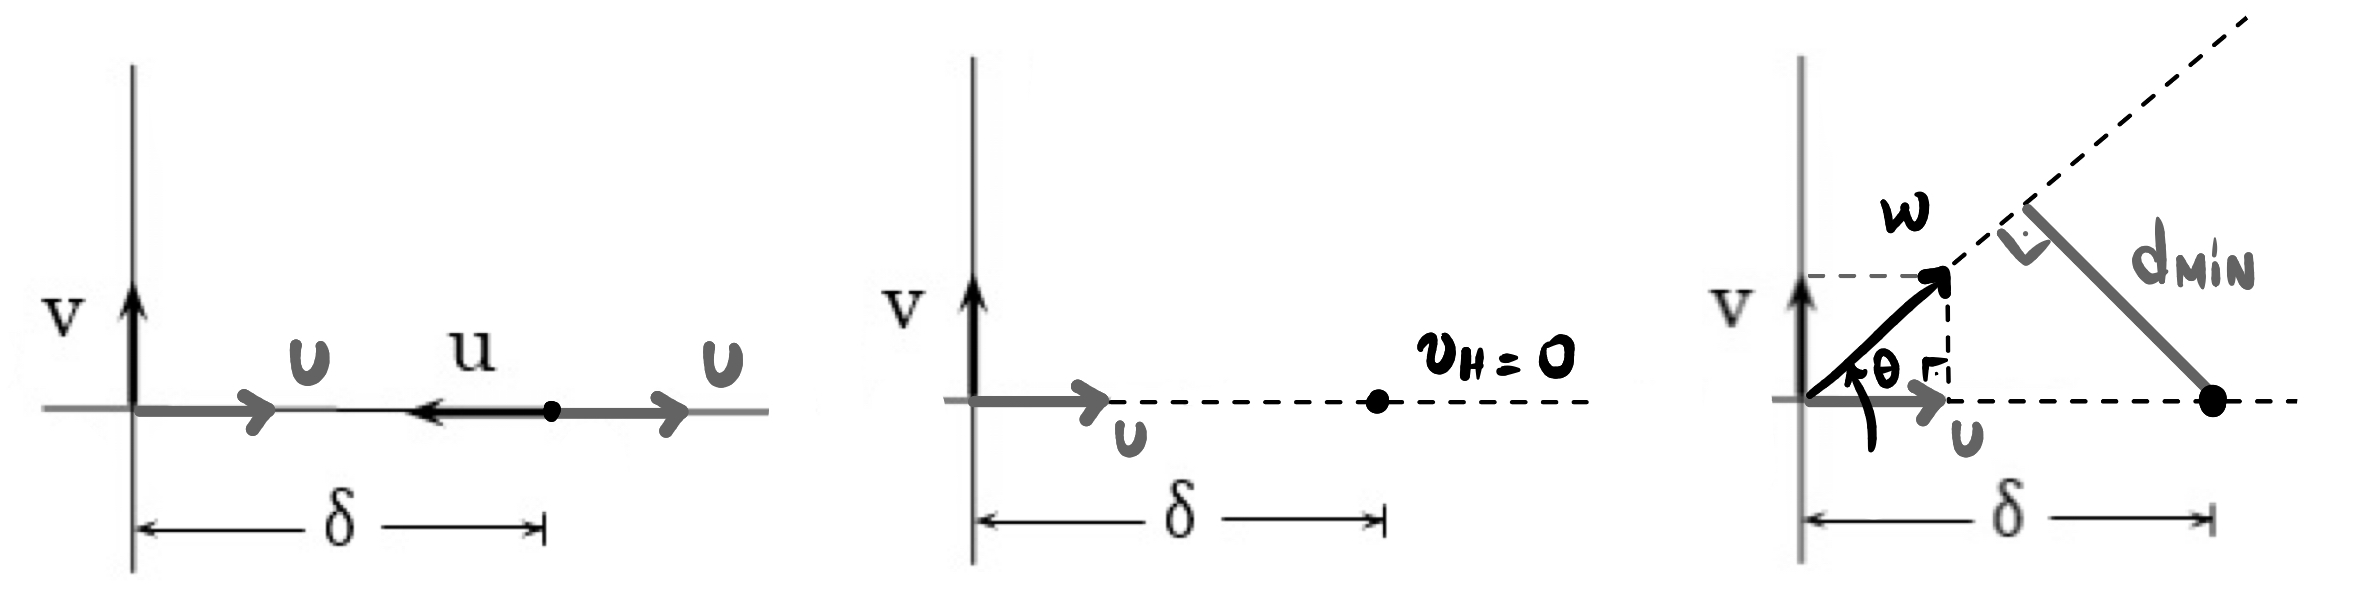
\includegraphics[width=0.80\linewidth]{imagensmecanica/mudancareferencialITA2d.jpeg}
% \captionof{figure}{}
% \label{fig_mec_mudancareferencialITA2d}
% } 


% A terceira imagem da figura mostra a trajetória do helicóptero no referencial do avião -- uma linha reta, inclinada de ângulo $\theta$ em relação à horizontal, sendo percorrida com velocidade $w$. Ora, no referencial do avião ele está parado, logo, a menor distância entre ele e o helicóptero será a menor distância entre um ponto e uma reta -- aquela tomada perpendicular à reta, destacada na terceira imagem da Figura \ref{fig_mec_mudancareferencialITA2d}. \\

% Podemos obter uma relação do $\sin \theta$ pelo trângulo dos vetores velocidade e o triângulo das distâncias, que fornecem, respectivamente:

% $$ \sin \theta =\dfrac{v}{w}= \dfrac{d_{min}}{\delta} \implies \boxed{d_{min}= \dfrac{ \delta v}{\sqrt{v^2+u^2}}.}$$

% Note que a distância entre dois pontos é uma propriedade geométrica invariante, ou seja, não depende do referencial -- a distância da ponta dos seus pés à sua cabeça é a sua altura, e este valor é o mesmo independente do referencial que o mede. Logo, a distância mínima entre os corpos obtida acima é uma grandeza absoluta, sendo, portanto, a mesma distância mínima que se obteria no referencial da terra. Com isso, eliminamos a alternativa E, que fornece o valor errado para tal distância. Vamos testar o que afirmam as outras alternativas:

% \begin{enumerate}
% \item [(a)] Para alcançar o ponto $O$ o avião leva um tempo $t'=\sfrac{\delta}{u},$ e, ao longo deste tempo, o helicóptero percorre uma distância dada por

% $$ d = vt'=  \dfrac{\delta v}{u},$$

% \noindent de modo que a alternativa $(a)$ também está errada.

%     \item [(b)] O tempo que demora até que se alcance a configuração em que a distância é mínima -- a situação da terceira imagem da Figura \ref{fig_mec_mudancareferencialITA2d} -- pode ser obtido fazendo a razão entre a distância percorrida pelo helicóptero neste referencial pela sua velocidade $w$ relativa ao mesmo referencial. A distância percorrida $x$ pode ser obtida por meio do $\cos \theta, $ pelo triângulo dos vetores velocidade e o trângulo de distâncias:

%     $$\cos \theta = \dfrac{u}{w} = \dfrac{x}{\delta} \implies x = \dfrac{\delta u}{\sqrt{v^2+u^2}},$$

%     \noindent de modo que o tempo para que isso ocorra é dado por 

%     $$ t = \dfrac{x}{w}=\dfrac{\delta u}{v^2+u^2},$$

%     \noindent de onde vemos que a letra $(d)$ está errada. Além disso, a distância do helicóptero ao ponto $O$ em tal instante é simplesmente

%     $$ d=vt= \dfrac{\delta uv}{v^2+u^2},$$

%     \noindent assim, a letra $(b)$ está errada.
    
    
%     Já a distância do avião ao ponto $O$ neste instante -- retornando ao referencial da terra -- é simplesmente dada por $(\delta - ut),$ haja vista que o helicóptero começa distando $\delta$ de tal ponto e se move com velocidade $u,$ no referencial da terra, em relação a ele. Logo, temos:

%     $$ \delta - ut = \delta - u\cdot \dfrac{\delta u}{v^2+u^2} = \dfrac{\delta v^2}{v^2+u^2},$$

%     \noindent de modo que a letra $(c)$ é a correta.



    
% \end{enumerate}


% \end{exemplo}



% \vspace{0.3cm}






\begin{exemplo}[Nível III (ITA 2009)]\label{exemplo_cinematica_vrelativa03}

Um barco leva 10 horas para subir e 4 horas para descer um mesmo trecho do rio Amazonas, mantendo constante o módulo de sua velocidade em relação à água. Quanto tempo o barco leva para descer esse trecho com os motores desligados?

\begin{enumerate}
    \item [a)] 14 horas e 30 minutos
    \item [b)] 13 horas e 20 minutos
    \item [c)] 7 horas e 20 minutos
    \item [d)] 10 horas
    \item [e)] Não é possível resolver porque não foi dada a distância percorrida pelo barco.
\end{enumerate}

\resolucao

Sejam $v$ o módulo da velocidade do barco em relação à água, $u$ o módulo da velocidade da correnteza e $d$ a extensão do trecho. Perceba que, com os motores desligados, o barco é carregado pela correnteza: sua velocidade em relação à margem é simplesmente $u$. Portanto, não precisamos encontrar $v$ nem $d$ separadamente — basta encontrar $u$.

Na subida, barco e correnteza se opõem, de modo que a velocidade resultante em relação à margem é $v - u$. Na descida com motores ligados, ambos cooperam, resultando em $v + u$. Usando $v=d/t$ em cada trecho:

$$v - u = \dfrac{d}{10}, \qquad v + u = \dfrac{d}{4}.$$

Subtraindo a primeira equação da segunda, eliminamos $v$:

$$2u = \dfrac{d}{4} - \dfrac{d}{10} = \dfrac{5d - 2d}{20} = \dfrac{3d}{20} \implies u = \dfrac{3d}{40}.$$

Com os motores desligados, o barco desce o trecho $d$ à velocidade $u$:

$$\Delta t = \dfrac{d}{u} = \dfrac{d}{\dfrac{3d}{40}} = \dfrac{40}{3} \text{ h} = \dfrac{39}{3} \text{ h} + \dfrac{1}{3} \text{ h}= 13\text{ h } 20\text{ min} \implies \text{letra B.}$$



\end{exemplo}

\vspace{0.3cm}



  











\begin{secnivel}[Aceleração Escalar Média]{I}{Aceleração Escalar Média}
  
  \eqLdois{def}{mecanica_eq_aceleracaomedia}{a_m := \dfrac{\Delta v}{\Delta t} }

\end{secnivel}
  






\secgfe{De onde vem}
O conceito de aceleração é criado a partir da necessidade de mensurar o quão rápido um movimento varia. Observe a situação Figura \ref{fig_mec_aceleracao01}. 

\begin{figure}[h]
    \centering
    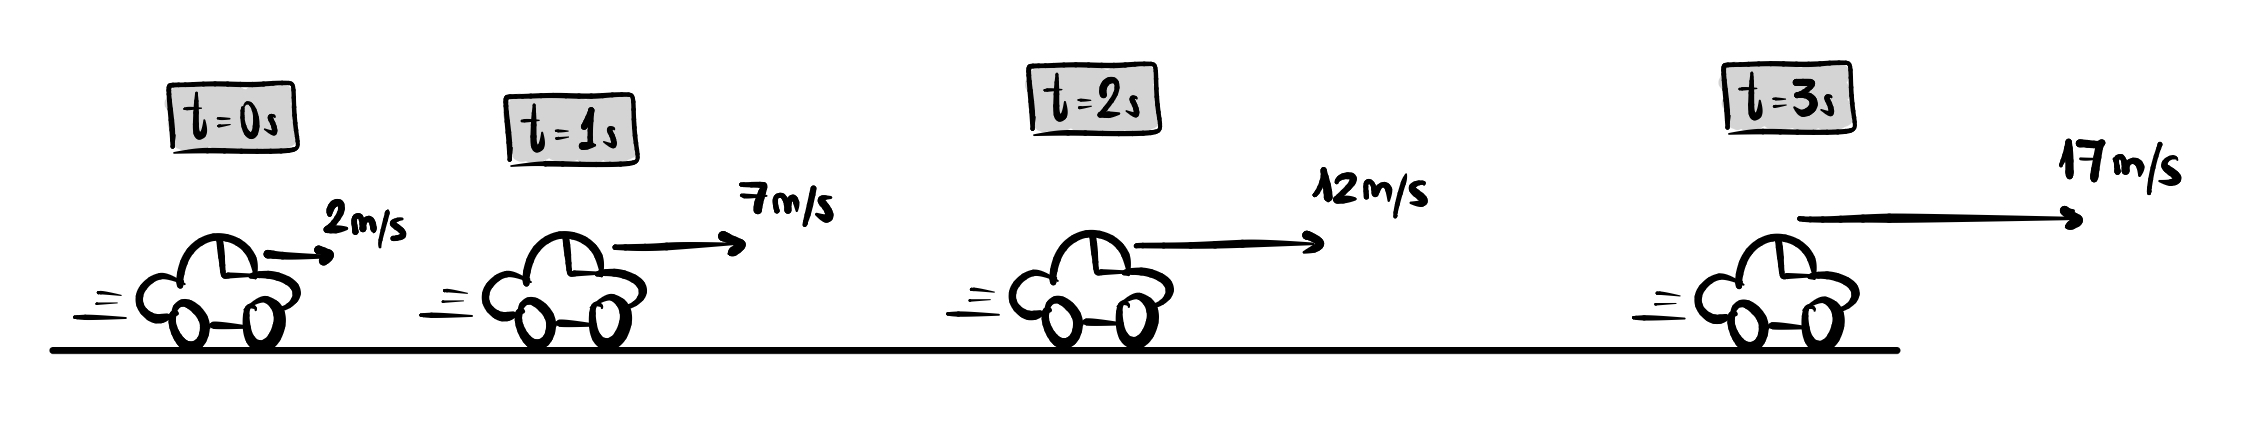
\includegraphics[scale=0.18]{imagensmecanica/acelerecao01.jpeg}
    \caption{Carro em movimento acelerado.}
    \label{fig_mec_aceleracao01}
\end{figure}



Como poderíamos comunicar a alguém acerca do que estamos vendo? Poderíamos dizer que estamos vendo um carro que anda cada vez mais depressa, com sua velocidade aumentando. Mas o quão mais depressa esse carro se move? Como essa velocidade aumenta?



%Poderíamos, é claro, simplesmente descrever o que vemos na figura: no instante inicial o carro possui velocidade de $2$ m/s; no instante $t=1s$ a sua velocidade é de $5$ m/s; no instante $t=2s$ a sua velocidade é de $12$ m/s e em $t=3s$ a sua velocidade é de $17$ m/s.



Para responder perguntas como essa é que estendemos o nosso vocabulário, introduzindo o conceito de aceleração, que irá medir justamente o quão rápido a velocidade está mudando à medida que tempo passa. Avaliando melhor o contexto, vemos, como mostra a Figura \ref{fig_mec_aceleracao02}, que há uma certa regularidade na forma como a velocidade varia: ela varia de exatamente $5$ m/s a cada segundo que passa, e a isso damos o nome de aceleração. Poderíamos dizer que o carro tem uma aceleração de $5$ m/s por segundo, ou seja, sua velocidade varia de $5$ m/s a cada segundo. Mas é mais comum dizermos que sua aceleração é de $5$ metros por segundo ao quadrado, ou $5\text{ m}/\text{s}^2,$ como pode ser destrinchado matematicamente:

$$ a = \dfrac{\Delta v}{\Delta t} = \dfrac{5\text{ m}/\text{s}}{1 \text{s}} = 5\text{ m}/\text{s}^2. $$



\begin{figure}[h]
    \centering
    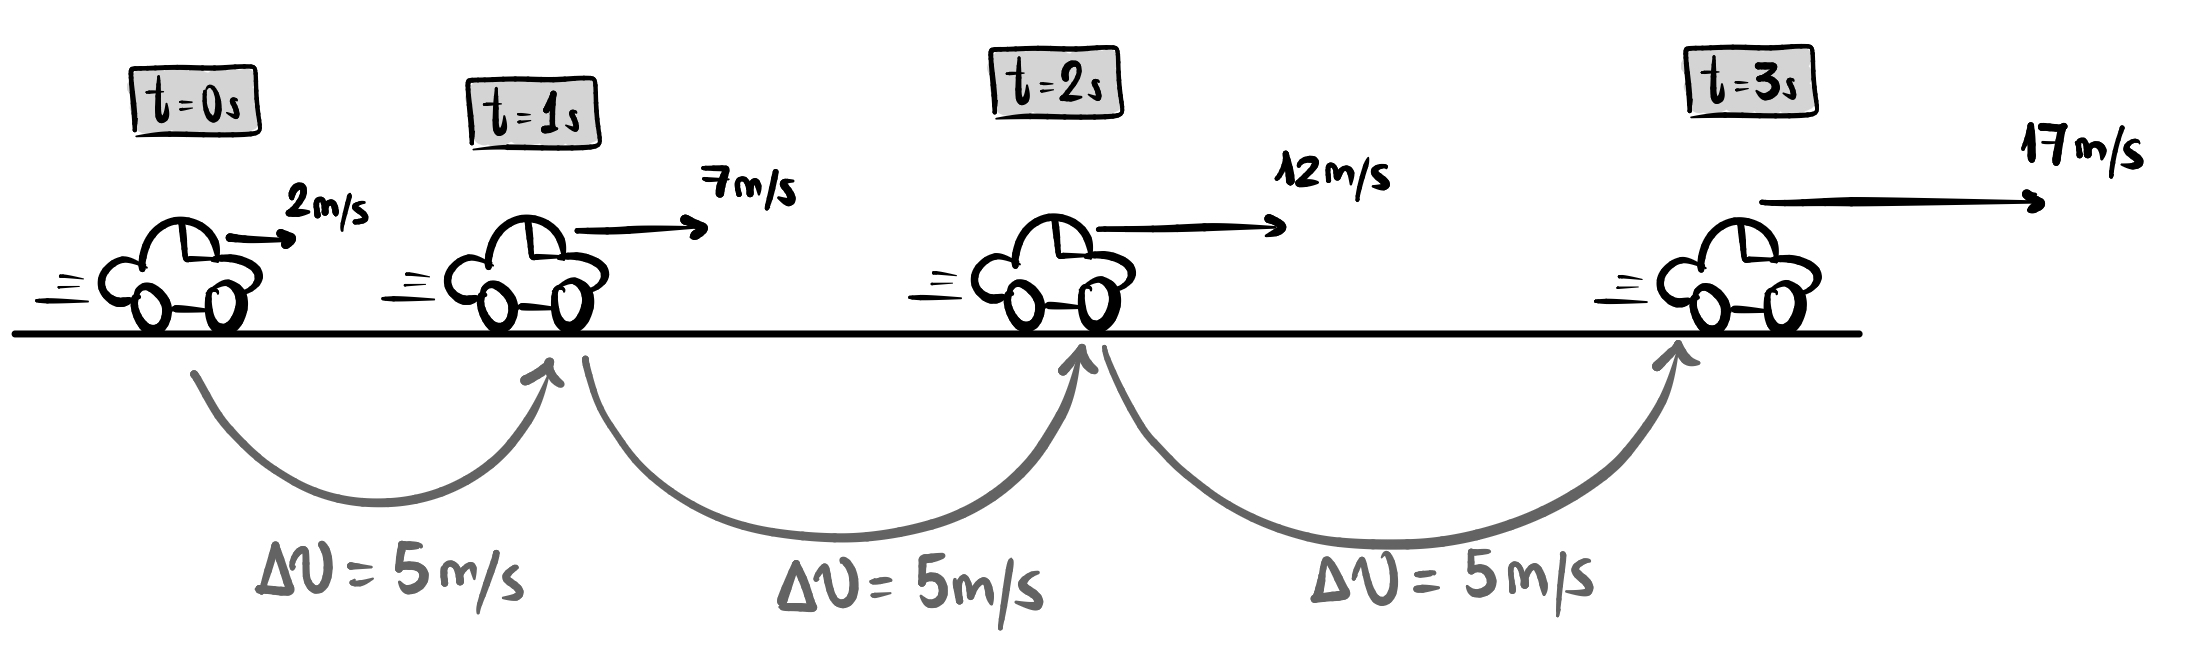
\includegraphics[scale=0.18]{imagensmecanica/acelerecao02.jpeg}
    \caption{Carro em movimento acelerado e o padrão de aumento de velocidade}
    \label{fig_mec_aceleracao02}
\end{figure}

Agora, munidos de tal conceito, temos mais vocabulário para estudar o movimento dos corpos -- em particular, corpos que se movem com velocidade variável.


\secgfe{Onde é usada}

Pode ser usada como uma aplicação direta para computar a aceleração de algum objeto que esteja se movendo. Por se tratar de uma equação que tem a ver com movimento -- ela mede o quão rápido o movimento (a velocidade) está mudando à medida que o tempo passa -- a aceleração irá aparecer em diversas fórmulas, como todas as de Cinemática, relativas ao movimento com aceleração constante, como:

$$ \Delta s = v_0t + \dfrac{1}{2}at^2 \quad ; \quad v^2 = v_0^2 + 2a\Delta s.$$

Além disso, como veremos futuramente, as forças são o que causam a aceleração dos corpos, de modo que a aceleração aparece na Segunda Lei de Newton:

$$ F = ma.$$


\secgfe{Erros comuns}

O erro mais comum certamente é confundir velocidade com aceleração. Para que fique bem claro: a velocidade mede o quão rápido um corpo de move, já a aceleração mede o quão rápido varia a velocidade desse mesmo corpo.

Desse modo, um corpo pode ter aceleração zero e ainda estar se movendo: se a aceleração é zero, significa que sua velocidade não varia, logo, tal corpo deve, necessariamente, estar se movendo com velocidade constante.

Portanto, atenção: se um corpo está em movimento ele \textbf{não precisa ter aceleração.} Se ele estiver em um movimento em que sua velocidade varia, aí sim ele precisa, \textbf{necessariamente}, ter aceleração.



\secgfe{Observações}

No Sistema Internacional de Unidades de Medida (SI) a unidade padrão para medir velocidade é o $\text{ m}/\text{s}$, e a unidade padrão para medida de tempo é o segundo, $\text{s}.$ Desse modo, a unidade padrão no (SI) para medir aceleração é, consequentemente, o $\text{ m}/\text{s}^2$.


É claro que alguém poderia medir a velocidade em $\text{km}/\text{h},$ o tempo em segundos, e computar uma aceleração medida em $\sfrac{\text{km/h}}{\text{s}}$, isso só seria muito estranho e bem pouco usual de ser feito.

\vspace{0.3cm}

\begin{exemplo}[Nível I]\label{exemplo_cinematicaescalar_aceleracaomedia01}


Considere um objeto, abandonado do repouso, a uma certa altura. Percebe-se que no terceiro segundo de seu movimento sua velocidade é de $12$ m/s. Já no quinto segundo do seu movimento sua velocidade é de $20$ m/s. Qual é a aceleração que tal objeto experimenta ao longo de seu movimento?



\resolucao



Usando a definição, e os valores de velocidade em $t_3=3$s e $t_5=5$s, temos que a aceleração média do objeto nestes 2 segundos de movimento foi

$$ a = \dfrac{\Delta v}{\Delta t} = \dfrac{v_5-v_3}{t_5-t_3}=\dfrac{20-12}{5-3} = \dfrac{8 \text{ m/s}}{2 \text{ s}} = 4 \text{m/s}^2.$$

  

    
\end{exemplo}

\vspace{0.3cm}




\begin{exemplo}[Nível II]\label{exemplo_cinematicaescalar_aceleracaomedia02}



Uma partícula move-se ao longo de uma trajetória retilínea orientada. Seu movimento ocorre em três intervalos de tempo consecutivos, de durações $\Delta t$, $2\Delta t$ e $3\Delta t$, respectivamente. As velocidades da partícula nos instantes inicial e final de cada intervalo são dadas a seguir:

\begin{itemize}
  \item [(i)] no instante inicial do primeiro intervalo, a velocidade vale $v$;
  \item [(ii)] no instante final do primeiro intervalo, a velocidade vale $2v$;
  \item [(iii)] no instante final do segundo intervalo, a velocidade vale $-v$;
  \item [(iv)] no instante final do terceiro intervalo, a velocidade vale $v$.
\end{itemize}

Não se dispõe de nenhuma outra informação sobre como a velocidade varia no interior de cada intervalo. Encontre a aceleração média da partícula durante o intervalo total de tempo.



\resolucao



Note que, para computar a aceleração média em um intervalo de tempo qualquer, tudo que precisamos é da velocidade $v_f$ no final de tal intervalo e da velocidade $v_0$ no início de tal intervalo. Toda e qualquer informação sobre velocidade durante tal intervalo é, portanto, irrelevante. \\

No caso do problema, as únicas informações importantes são aquelas dos itens $(i)$ e $(iv)$ -- a velocidade inicial no início de todo o movimento e a velocidade final no final do último trecho -- todo o resto é distração. Assim, ao longo de todo o trecho de duração $\Delta t+ 2\Delta t+3\Delta t = 6\Delta t$, a aceleração média é

$$ a_m = \dfrac{\Delta v}{\Delta t} = \dfrac{v_f-v_0}{6 \Delta t} = \dfrac{v-v}{6 \Delta t} = 0.$$

  

    
\end{exemplo}



\vspace{0.3cm}






















\newpage





\section{Movimento Uniforme}

O Movimento Uniforme (MU) é aquele no qual a velocidade possui valor constante. Observe, por exemplo, a Figura \ref{fig_mec_mu01}, que mostra um movimento uniforme unidimensional: o tempo passa e o valor de velocidade é sempre exatamente o mesmo (4 m/s, neste caso). Isso é o que caracteriza um movimento uniforme: o corpo percorre distâncias iguais em intervalos de tempos iguais, ou, caso o leitor prefira, a distância percorrida é sempre diretamente proporcional ao tempo transcorrido.


\begin{figure}[h]
    \centering
    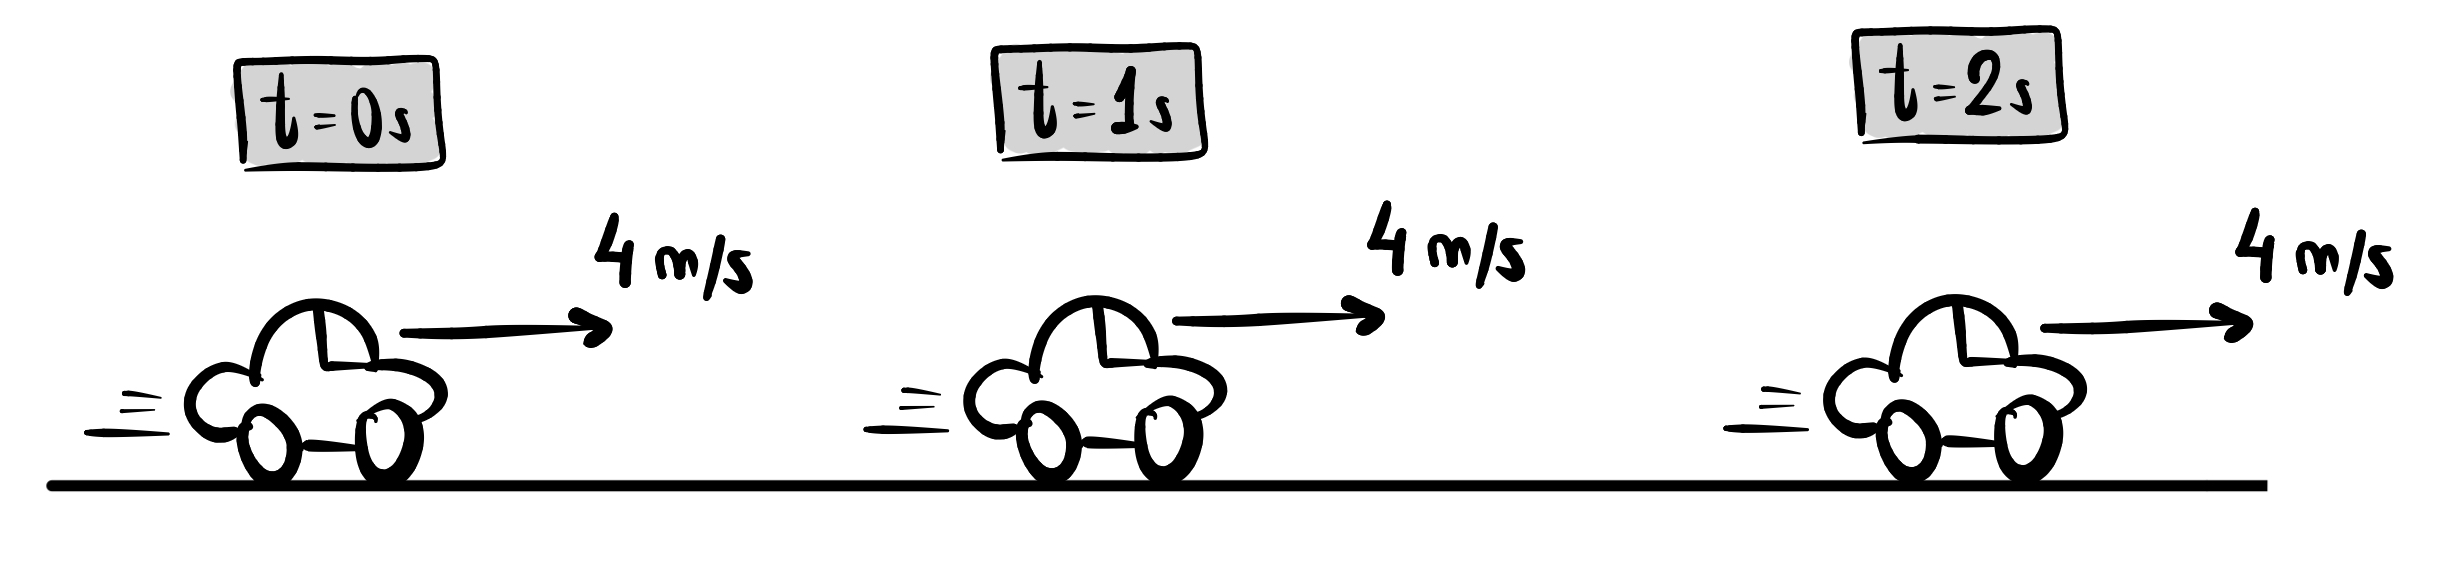
\includegraphics[scale=0.12]{imagensmecanica/mu01.jpeg}
    \caption{O Movimento Uniforme.}
    \label{fig_mec_mu01}
\end{figure}

Note, contudo, que o caso da Figura \ref{fig_mec_mu02} não constitui um MU, como talvez alguém poderia pensar, haja vista que o valor da velocidade é sempre de $4$ m/s. Não se trata de um MU, e vamos destacar dois aspectos que evidenciam isso:

\begin{itemize}
    \item [(i)] Note que, para que se alcance o cenário em $t=2$s, seria preciso que a velocidade do carro, a partir de $t=1s$, fosse diminuindo, até zerar. A partir deste momento o carro conseguiria inverter o sentido do seu movimento, começando a acelerar no sentido oposto, aumentando o valor de sua velocidade até alcançar o valor de $4$ m/s.

    Ou seja, o movimento foi acelerado entre $t=1$s e $t=2$s: a velocidade não ficou constante, de modo que não se trata de um MU.


    \item [(ii)] Dada a discussão do tópico anterior, está claro como que uma velocidade de $4$ m/s apontando para a direita é diferente de uma velocidade de $4$ m/s apontando para a esquerda -- e que deve haver aceleração para sair de uma configuração para outra.

    Dito isso, como faremos para não confundir essas duas situações? A Figura \ref{fig_mec_mu02} deixa isso claro: ao adotar um eixo de referência para marcar posições (um referencial), imediatamente isso já define um sentido positivo -- o sentido no qual as posições crescem -- e um sentido negativo -- o sentido no qual as posições diminuem.\footnote{Caso o leitor não tenha se dado conta de que isso é imediato, perceba que trata-se apenas de uma consequência da forma como definimos a velocidade. Considere as posições $10$m e $12$m, e um MU entre as duas que dura $1$s. Um corpo que sai de $s_0=10$m para $s_f=12$m terá velocidade média dada por $\sfrac{\Delta s}{\Delta t}=\sfrac{(12-10)}{1}=+2\text{m/s}$; já um corpo que sai de $s_0=12$m para $s_f=10$m terá velocidade média dada por $\sfrac{\Delta s}{\Delta t}=\sfrac{(10-12)}{1}=-2\text{m/s}$. Ou seja, quando nos movemos no sentido em que as posições diminuem a velocidade automaticamente já aparece com sinal negativo no cálculo -- o contrário também sendo verdadeiro. Logo, o fato da velocidade positiva ser aquela que aponta no sentido crescente das posições e a velocidade negativa ser aquela que aponta no sentido decrescente das posições é apenas uma consequência de como a velocidade média é definida, e não um fato extra que inserimos artificialmente na teoria. Esses dois movimentos, inclusive, recebem nomes: movimento progressivo -- quando a velocidade é positiva, ou seja, o corpo progride no eixo das posições -- e movimento retrógrado -- quando a velocidade é negativa, ou seja, o corpo retrocede no eixo das posições. } Desse modo, uma velocidade que aponte para a direita será considerada positiva, enquanto uma velocidade que aponta para a esquerda será considerada negativa. Assim, podemos diferenciar as duas situações, e fica claro que $+4$ m/s indica uma velocidade para a direita enquanto que $-4$ m/s indica uma velocidade para a esquerda.

    Isso também vale para acelerações -- uma aceleração negativa quer dizer simplesmente que ela aponta para o sentido contrário em que as posições crescem. Dito isso, é importante ressaltar: \textbf{o sinal de grandezas como velocidade e aceleração na cinemática está relacionado unicamente ao sentido no qual tais grandezas apontam, e é usado, justamente, para diferenciar corpos que se movem em sentidos opostos ao longo de uma mesma direção.}\footnote{Vale lembrar que o sentido em que as coisas crescem é arbitrário -- depende da escolha que se faça.}
\end{itemize}





\begin{figure}[h]
    \centering
    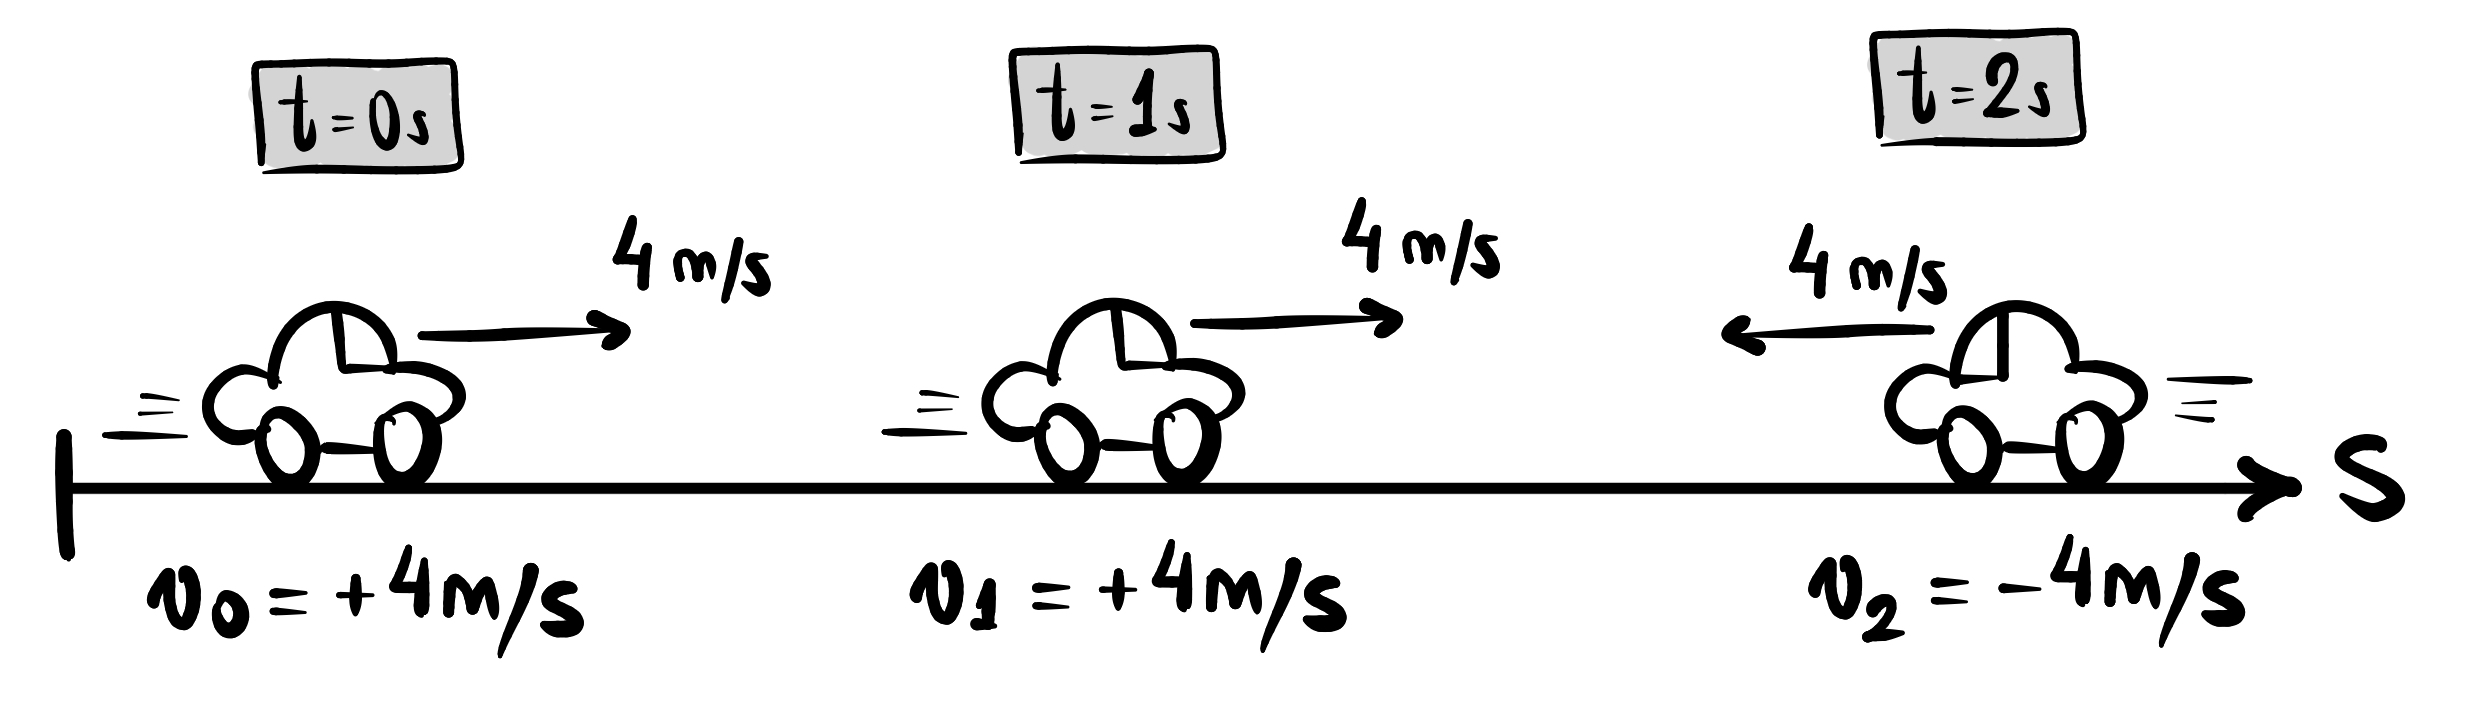
\includegraphics[scale=0.12]{imagensmecanica/mu02.jpeg}
    \caption{O sinal de uma grandeza física como velocidade ou aceleração está relacionado ao sentido em que tal grandeza aponta.}
    \label{fig_mec_mu02}
\end{figure}



\begin{secnivel}[Distância no Movimento Uniforme]{I}{Distância no Movimento Uniforme}
 

  \eqLdois{dem}{mecanica_eq_distanciamu}{d=vt}
  
\end{secnivel}







\secgfe{De onde vem}

Essa talvez seja a equação mais básica de toda a Física, e serve para calcular a distância percorrida por um corpo que executa um Movimento Uniforme.

Ela é uma consequência imediata da definição de velocidade média, feita na Equação \eqref{mecanica_eq_velocidademedia}. Note que, se temos um MU, isso significa que a velocidade é constante o tempo inteiro, por definição. Isso quer dizer, consequentemente, que o sentido do movimento nunca muda, isto é, se o corpo se move inicialmente para a direita, como mostra Figura \ref{fig_mec_mu01}, ele irá se mover para direita ao longo de todo o movimento -- caso contrário, para inverter o sentido do movimento, o corpo teria que acelerar, como vimos na situação da Figura \ref{fig_mec_mu02}, de modo que isso descaracterizaria o MU.

Dito isso, cabe ao leitor lembrar da nossa discussão feita na definição da Equação \eqref{mecanica_eq_velocidademedia} sobre a diferença entre o deslocamento $\Delta s$ e a distância percorrida $d$. Deixamos claro que essas duas grandezas deixam de coincidir quando há inversão no sentido do movimento. Logo, no MU, como isso nunca ocorre, distância e deslocamento sempre coincidirão, de modo que, a partir da Equação \eqref{mecanica_eq_velocidademedia}, podemos escrever

$$ v_m = \dfrac{\Delta s}{\Delta t} = \dfrac{d}{t-0} \implies v_m = \dfrac{d}{t},$$

\noindent em que escolhemos o instante inicial do movimento como sendo $t_0=0.$ Ora, como a velocidade no MU é constante, a velocidade média, $v_m$, em qualquer intervalo de tempo analisado irá sempre coincidir com a velocidade, $v$, do carro -- que é sempre a mesma. Logo, $v_m=v,$ de modo que a equação acima se torna

$$ v_m=v=\dfrac{d}{t} \implies \boxed{ d=vt,}$$

\noindent e está provado que, no MU, a distância é igual ao produto da velocidade pelo tempo. É importante que o leitor note que o argumento principal para que isso funcionasse estava pautado em dois critérios:

\begin{itemize}
    \item [(i)] O deslocamento $\Delta s$ e a distância percorrida $d$ coincidem para um corpo que executa um Movimento Uniforme, isto é:

    $$\Delta s = d.$$

    \item [(ii)] A velocidade $v$ do corpo, no MU, é sempre exatamente a mesma, de modo que ela coincide com a velocidade média em qualquer intervalo de tempo que se analise, ou seja:

    $$ v_m = v.$$
\end{itemize}

Esses dois critérios serão sempre atendidos exclusivamente para o MU, de modo que a Equação \eqref{mecanica_eq_distanciamu} será válida apenas para um corpo que executa um MU.


\secgfe{Onde é usada}

Em problemas que envolvem corpos que se movam com velocidade constante.



\secgfe{Erros comuns}

Essa, como dito, é uma das equações mais simples da física, de modo que não deixa tanta margem para que se cometa muitos erros que não sejam erros simples de cálculos matemáticos.

Talvez o principal erro aqui seja o estudante acreditar que essa é a equação fundamental do movimento de toda a Física, ou seja, que ela vale para qualquer tipo de movimento. Isso está, claramente, errado, e fizemos questão de evidenciar que a Equação \eqref{mecanica_eq_distanciamu} vale apenas para um corpo que executa um Movimento Uniforme. Caso o leitor queira aplicar tal equação para calcular a distância percorrida por um carro que acelera, ou que desacelera, ou qualquer outro tipo de movimento que não seja o MU, a equação irá fornecer certamente valores errados, por não se aplicar em tais regimes.



\secgfe{Observações}

A observação mais relevante aqui talvez seja a de que, em muitos problemas, o uso direto da Equação \eqref{mecanica_eq_distanciamu} pode acabar sendo o caminho mais complicado para resolver o problema. Em muitos problemas de Cinemática que envolvem o MU, a situação é drasticamente simplificada caso, primeiro, usemos a Equação \eqref{mecanica_eq_velocidaderelativa} para escolher o referencial adequado e, só então, usemos a Equação \eqref{mecanica_eq_distanciamu}. Isso ficará claro em alguns exemplos que resolveremos a seguir.





\vspace{0.3cm}


\begin{exemplo}[Nível I]\label{exemplo_distanciamovuniforme01}

Um carro se move com velocidade constante de 20 m/s ao longo de uma rodovia, enquanto outro se move com velocidade constante de 30 m/s, em sentido oposto, ao longo da mesma rodovia.

Se os carros inicialmente estão separados por uma distância de 1.2 km, após quanto tempo eles irão passar um pelo outro?

\resolucao

Vamos resolver esse problema de duas formas, mudando apenas o referencial.

\begin{itemize}
    \item [(i)] Referencial da Terra.

    A Figura \ref{fig_mec_muexemplo01} mostra a situação, em que os carros $A$ e $B$ estão separados de $1200$m. Digamos que eles vão se encontrar no ponto $P$, que, naturalmente, estará mais próximo de onde estava inicialmente o carro $A$, uma vez que este se move com uma velocidade menor.

    Sejam $d_A$ e $d_B$ as distâncias que os carros $A$ e $B,$ respectivamente, devem percorrer até chegar ao ponto de encontro $P$. Ora, tais distâncias devem varrer, somadas, a distância de $1200$m que inicialmente os separava, como a figura evidencia. Ou seja, matematicamente:

    $$ d_A + d_B = 1200.$$

    Sendo os movimentos uniformes, podemos usar a Equação \eqref{mecanica_eq_distanciamu} para cada um deles, ou seja, $d_A=v_A\cdot t = 20t$ e $d_B=v_b \cdot t = 30t,$ que, na equação acima, fornece:\footnote{Talvez o leitor pode ter ficado com a dúvida se a velocidade do carro que anda em sentido contrário não deveria ter entrado com sinal negativo na equação. Vamos discutir isso, em mais detalhes, na seção sobre a Equação \eqref{mecanica_eq_mu_funcaoposicao}.}

    $$ 20t + 30 t = 1200 \implies 50t=1200 \implies \boxed{t=24 \text{ segundos.}}$$



 {
\centering
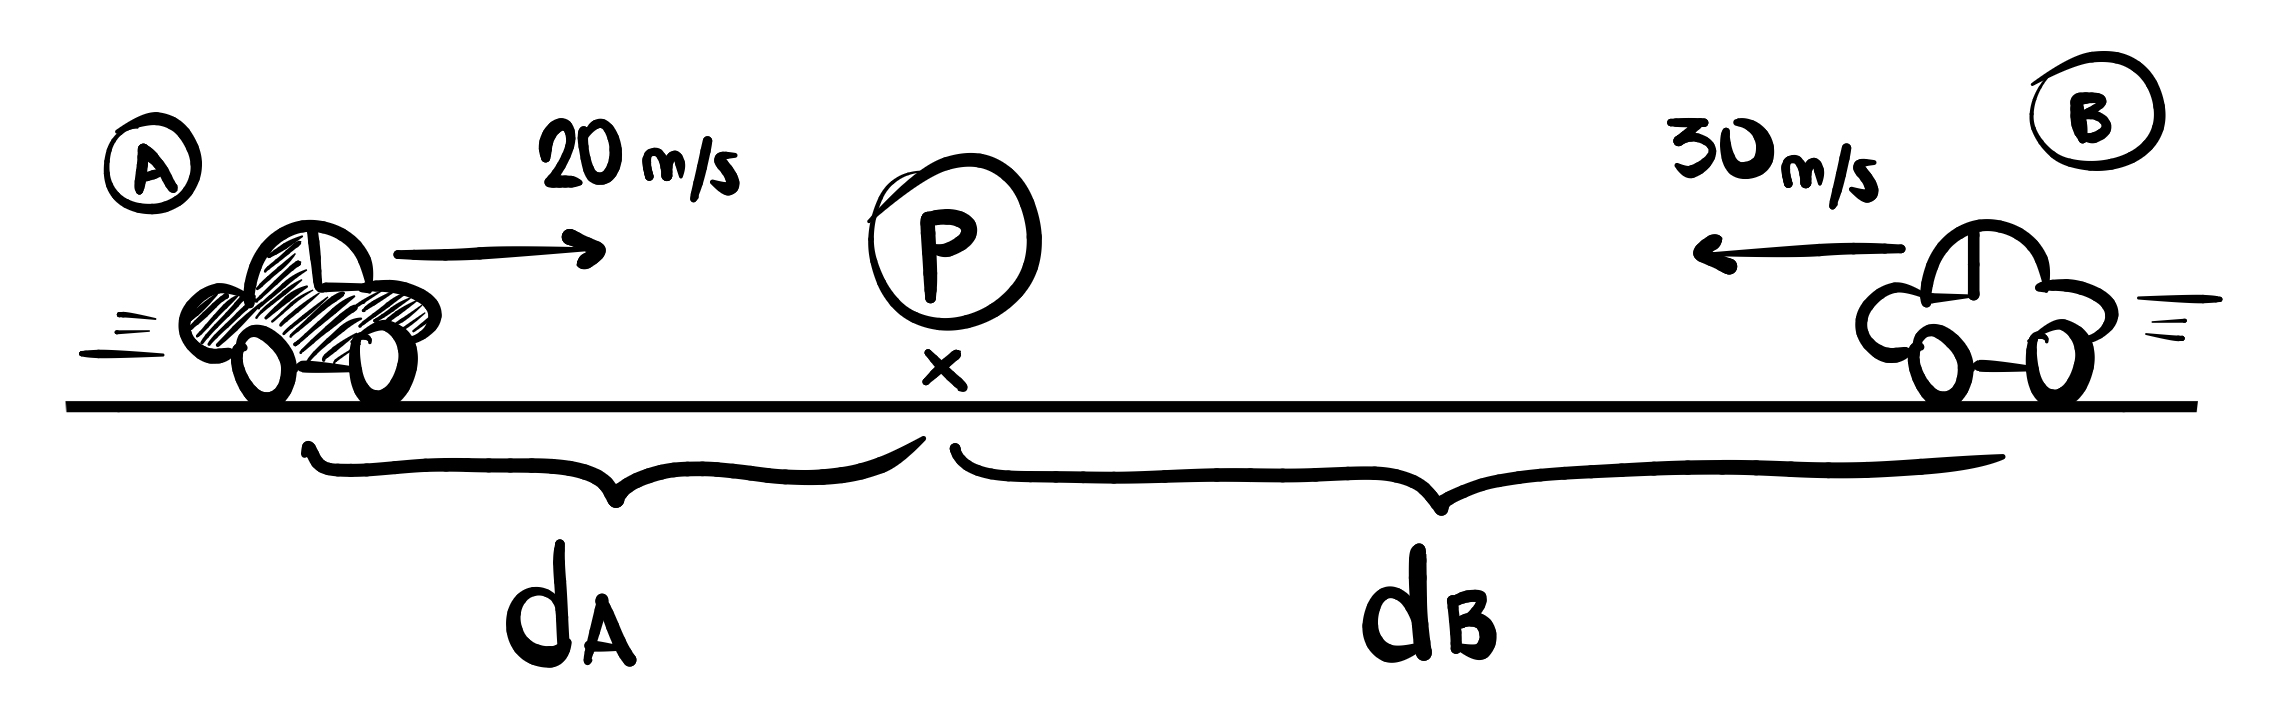
\includegraphics[width=0.6\linewidth]{imagensmecanica/muexemplo01.jpeg}
\captionof{figure}{}
\label{fig_mec_muexemplo01}
} 


    \item[(ii)] Referencial do carro $B$.

    Essa solução envolve fazer uma mudança de referencial, como aprendemos na construção da Equação \eqref{mecanica_eq_velocidaderelativa}. A Figura \ref{fig_mec_muexemplo0102} mostra, inicialmente, a situação no referencial da terra e, em seguida, a situação no referencial do carro $B.$ Lembrando que, para fazermos tal mudança, adiciona-se o oposto da velocidade de $B$ a todas as partículas do sistema, o que o faz ficar parado. Com isso, a velocidade do carro $A$ em relação ao carro $B$ é de $50$ m/s, como mostra a figura.


 {
\centering
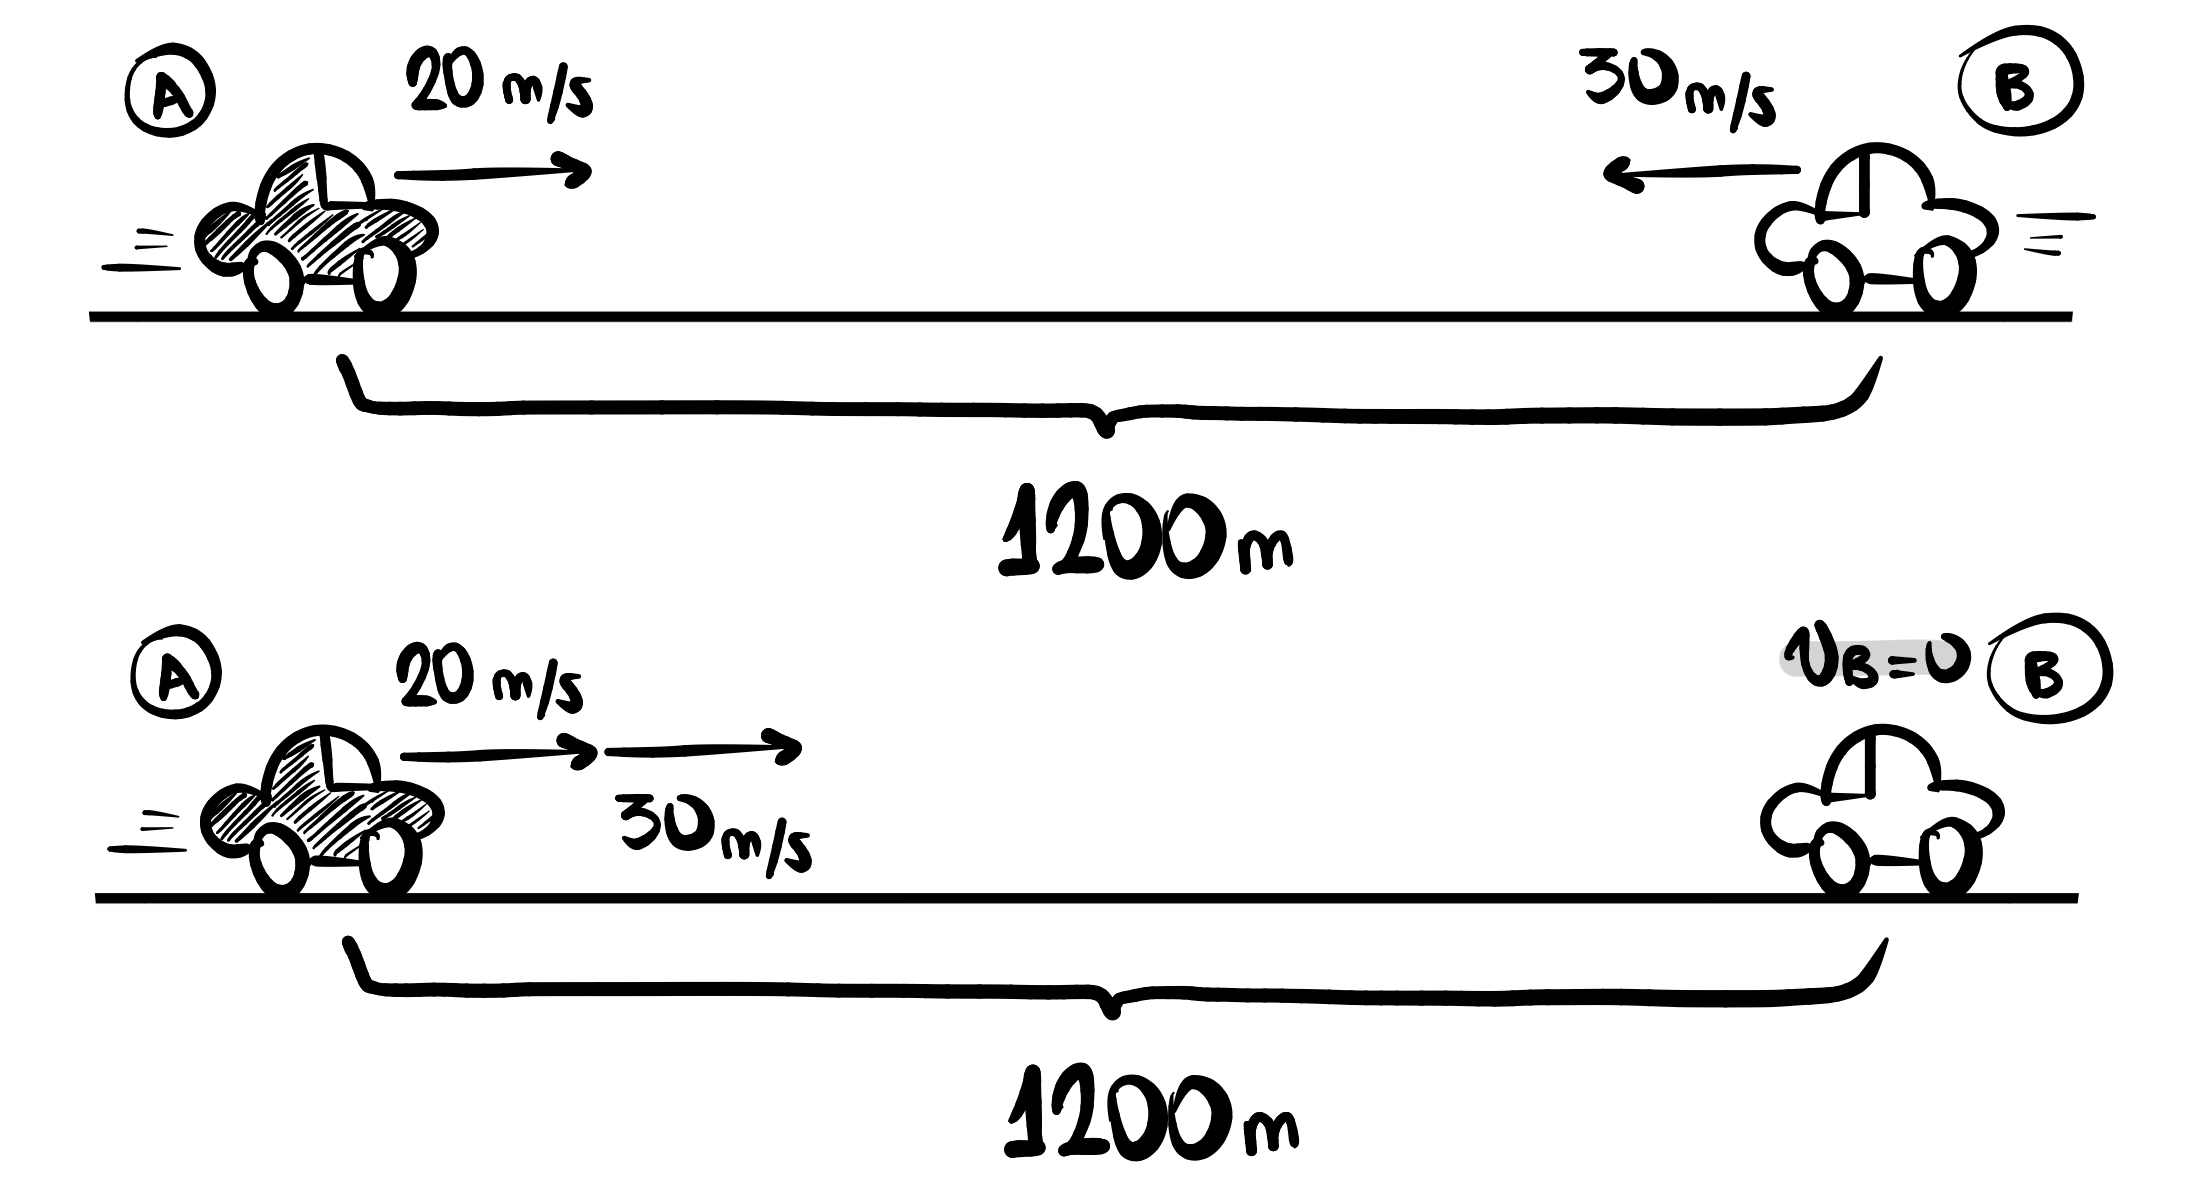
\includegraphics[width=0.6\linewidth]{imagensmecanica/muexemplo0102.jpeg}
\captionof{figure}{}
\label{fig_mec_muexemplo0102}
} 



Perceba que, agora, o problema ficou substancialmente mais simples: temos um carro que se move a $50$ m/s em direção a um outro carro, parado, que está afastado de $1200$m do primeiro. Sendo assim, o tempo que demora até que um carro encontre o outro é dado de forma direta por

$$ d = v \cdot t \implies 1200 = 50 t \implies \boxed{t = 24 \text{ segundos.}}$$

    
\end{itemize}

Note que, escolhendo o referencial adequado, o problema fica mais simples e, consequentemente, seus cálculos e sua resolução também. É sempre mais fácil resolver um problema de Cinemática em que há apenas um corpo em movimento e o outro fica parado. Quando os dois ou mais corpos se movem, a analise e os cálculos costumam ficar mais laboriosos -- é por isso que a mudança de referencial da segunda solução simplificou o problema. 


\end{exemplo}


\vspace{0.3cm}






\begin{exemplo}[Nível II]\label{exemplo_distanciamovuniforme02}


Dois trens partem, simultaneamente, um em direção ao outro, com velocidade constante de 80 km/h. O trem 1 sai da cidade A em direção à cidade B, enquanto o trem 2 sai da cidade B para a cidade A. A distância entre as cidades é de 640 km.

Uma mosca, inicialmente pousada na dianteira do trem 1, se move em direção à dianteira do trem 2. Ao chegar lá, ela imediatamente retorna até à dianteira do trem 1, e assim continua, até morrer esmagada pela colisão dos dois trens. Se a velocidade da mosca é de 120 km/h, qual é a distância total que ela percorre até ser esmagada?

\resolucao





Este problema, em um primeiro momento, pode parecer bastante complicado -- mas ele é bem parecido com o problema anterior. Note que a dificuldade parece residir no fato de que a mosca fica o tempo inteiro pulando de um lado para o outro -- isso enquanto os dois trens se aproximam um do outro, de modo que suas posições mudam e a mosca vai e volta cada hora até um lugar diferente.
\\

De fato é bem difícil avaliar o movimento da mosca. Contudo, isso não é necessário. Note que, a velocidade da mosca sendo constante, podemos usar que $d=v \cdot t.$ Como sabemos sua velocidade $v$, basta descobrirmos por quanto tempo $t$ ela ficará se movendo que será imediato obter a distância total $d$ que ela percorre. Ora, mas o tempo que ela se move é exatamente o tempo necessário para que os trens se encontrem, e isso é exatamente o que fizemos no problema anterior.

Mudando para o referencial de um dos trens, um ficará parado e o outro se moverá a uma velocidade de $80+80 = 160$ km/h, que, para varrer uma distância de $640$ km até colidir com o outro, levará um tempo de
$$ d= v \cdot t \implies 640 \text{ km} = 160 \text{ km/h} \cdot t \implies \boxed{t=4 \text{ h.}}$$

Assim, se a mosca se move por $4$ horas com uma velocidade de $120$ km/h, ela percorrerá, ao longo de todo o seu movimento, uma distância igual a

$$ d = vt = 120 \cdot 4 = \boxed{480 \text{ km.}}$$

\end{exemplo}


\vspace{0.3cm}






\begin{exemplo}[Nível III (ITA - 2007)]\label{exemplo_distanciamovuniforme03}


Considere que num tiro de revólver, a bala percorre trajetória retilínea com velocidade $v$ constante, desde o ponto inicial P até o alvo Q. 


 {
\centering
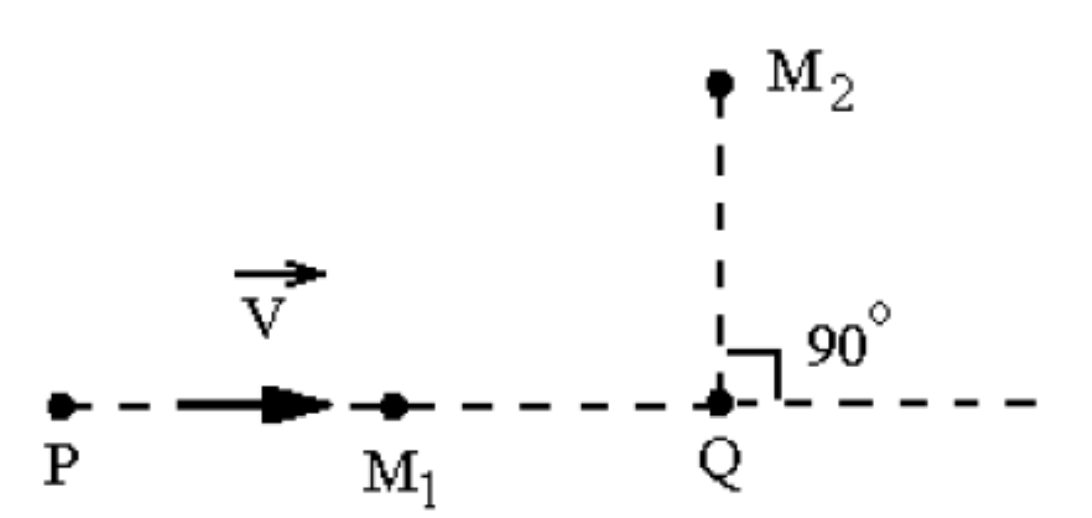
\includegraphics[width=0.35\linewidth]{imagensmecanica/muexemplo03ita.png}
\captionof{figure}{}
\label{fig_mec_muexemplo03ita2007}
} 



Mostrados na figura, o aparelho M$_1$ registra simultaneamente o sinal sonoro do disparo e o do impacto da bala no alvo, o mesmo ocorrendo com o aparelho M$_2$. Sendo $v_s$ a velocidade do som no ar, então a razão entre as respectivas distâncias dos aparelhos M$_1$ e M$_2$ em relação ao alvo
Q é

\begin{enumerate}
    \item [(a)] $\dfrac{v_s(v-v_s)}{v^2-v_s^2}$
    \item [(b)] $\dfrac{v_s(v_s-v)}{v^2-v_s^2}$
    \item [(c)] $\dfrac{v(v-v_s)}{v_2^2-v^2}$
    \item [(d)] $\dfrac{v_s(v\cdot v_s)}{v^2-v_s^2}$
    \item [(e)] $\dfrac{v_s(v-v_s)}{v^2\cdot v_s^2}$
\end{enumerate}

\resolucao


Considere as distâncias $x$, $y$ e $D$ nomeadas na Figura \ref{fig_mec_muexemplo03ita2007solution}. O que o enunciado nos pede é o valor da razão $\sfrac{x}{y}.$



 {
\centering
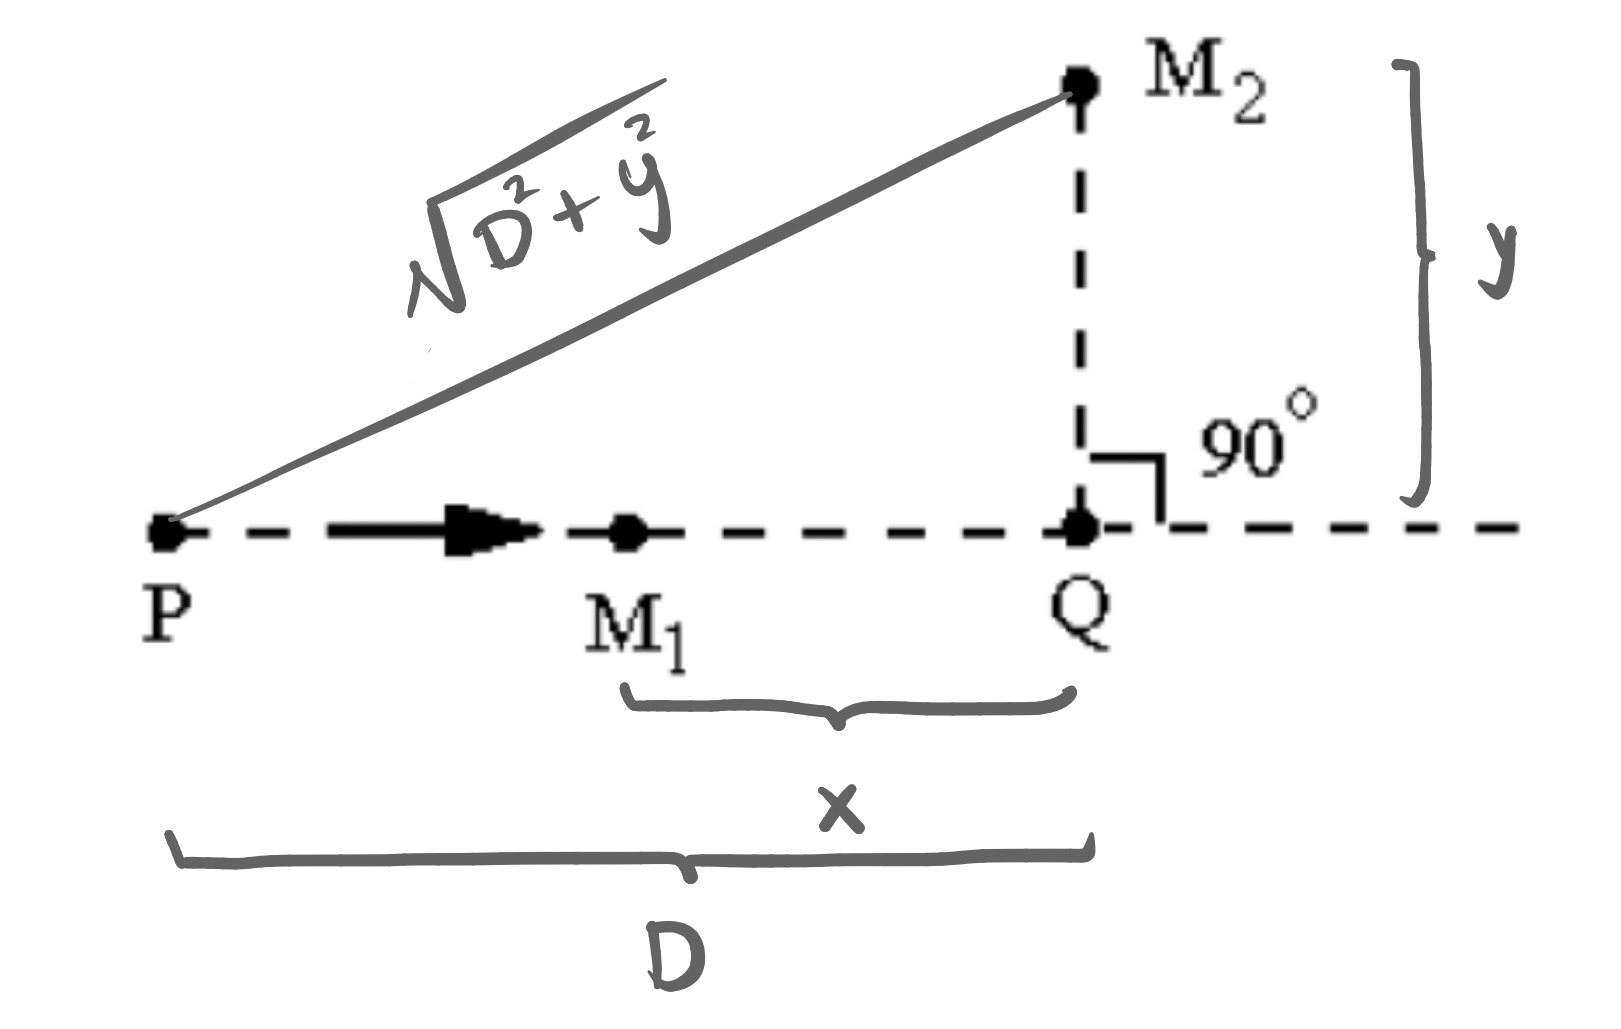
\includegraphics[width=0.4\linewidth]{imagensmecanica/muexemplo03itaresolucao.jpeg}
\captionof{figure}{}
\label{fig_mec_muexemplo03ita2007solution}
} 


Computemos primeiro os tempos para o aparelho $M_1$. Teremos:

\begin{enumerate}
    \item [(i)] Tempo para receber o som do disparo, isto é, para o som do disparo viajar de $P$ até $M_1$: $t_1 = \sfrac{(D-x)}{v_s}.$

    \item [(ii)] Tempo para receber o som do impacto da bala no alvo.

    Para isso, a bala precisa chegar ao alvo, isto é, viajar de $P$ até $Q$, o que leva um tempo $t'=\sfrac{D}{v}.$ Em seguida, o som do impacto deve viajar de $Q$ até $M_1,$ o que leva um tempo $t''=\sfrac{x}{v_s},$ totalizando um tempo total $t_2=t'+t''= \sfrac{(Dv_s+xv)}{(v \cdot v_s)}.$
\end{enumerate}

O enunciado nos diz que o aparelho $M_1$ registra simultaneamente os dois sons, ou seja, os tempos $t_1$ e $t_2$ calculados acima são iguais:

$$ \dfrac{(D-x)}{v_s} = \dfrac{Dv_s+xv}{v\cdot v_s}  \implies \boxed{(D-x) v = Dv_s+xv.}$$

Note que multiplicamos os dois lados da equação por $v \cdot v_s$ a título de simplificação. Agora, para o aparelho $M_2,$ precisamos também computar dois intervalos de tempo. Da tal equação tiramos que 

\begin{equation}
 \boxed{x=\dfrac{D(v-v_s)}{2v}}    
 \label{eq_cinematica_mu_questaoITA01}
\end{equation}


\begin{enumerate}
    \item [(i)] Tempo para receber o som do disparo, isto é, para o som do disparo viajar de $P$ até $M_2$: $t_3 = \sfrac{\sqrt{D^2+y^2}}{v_s}.$

    \item [(ii)] Tempo para receber o som do impacto da bala no alvo.

    Para isso, a bala precisa chegar ao alvo, isto é, viajar de $P$ até $Q$, o que leva um tempo $t'=\sfrac{D}{v}.$ Em seguida, o som do impacto deve viajar de $Q$ até $M_2,$ o que leva um tempo $t''=\sfrac{y}{v_s},$ totalizando um tempo total $t_4=t'+t''= \sfrac{(Dv_s+yv)}{(v \cdot v_s)}.$
\end{enumerate}

O enunciado nos diz que o aparelho $M_2$ registra simultaneamente os dois sons, ou seja, os tempos $t_3$ e $t_4$ calculados acima são iguais:

$$ \dfrac{\sqrt{D^2+y^2}}{v_s} = \dfrac{Dv_s+yv}{v\cdot v_s}  \implies \boxed{v\sqrt{D^2+y^2}  = Dv_s+yv.} $$

Elevando os dois membros dessa última equação ao quadrado, teremos: 


\begin{align}
    v^2(D^2+y^2)&=D^2v_s^2+2Dyv_sv+y^2v^2 \nonumber \\
    v^2D^2+ \cancel{v^2y^2} &=D^2v_s^2+2Dyv_sv+ \cancel{y^2v^2} \nonumber
\end{align}

\noindent e, isolando $y$,
chegaremos em 





\begin{equation}
 \boxed{y = \dfrac{D(v^2-v_s^2)}{2vv_s}} 
 \label{eq_cinematica_mu_questaoITA02}
\end{equation}



Assim, dividindo a Equação \eqref{eq_cinematica_mu_questaoITA01} pela Equação \eqref{eq_cinematica_mu_questaoITA02}, obtemos a razão que o enunciado pede:

$$ \boxed{\dfrac{x}{y}=\dfrac{v_s(v-v_s)}{v^2-v_s^2} \implies \text{Letra A.}}$$

\end{exemplo}


\vspace{0.3cm}





















\begin{secnivel}[Função Horária da Posição no MU]
{I}{Função Horária da Posição no Movimento Uniforme}
 

  \eqLdois{dem}{mecanica_eq_mu_funcaoposicao}{s=s_0+vt}
  
\end{secnivel}
  








\secgfe{De onde vem}
Essa equação segue naturalmente da definição de velocidade média feita na Equação \eqref{mecanica_eq_velocidademedia}. Façamos a análise de um movimento a partir do instante inicial $t_0=0,$ no qual a posição do móvel é $s_0.$ Assim, da equação \eqref{mecanica_eq_velocidademedia} temos:

$$ v_m = \dfrac{\Delta s}{\Delta t} = \dfrac{s-s_0}{t-0} \implies s = s_0 + v_mt,$$
contudo, como discutimos anteriormente, no MU a velocidade é sempre a mesma, coincidindo, portanto, sempre com a sua velocidade média: $v=v_m.$ Assim, a equação acima se reduz a

$$ \boxed{s=s_0+vt.}$$




\secgfe{Onde é usada}

Em problemas que envolvem corpos que se movam com velocidade constante. Em geral, ela pode ser usada para resolver os mesmos problemas que resolvemos no tópico anterior, usando a Equação \eqref{mecanica_eq_distanciamu}. De modo geral, ela acaba sendo mais útil em problemas nos quais deseja-se saber, por exemplo, a posição de encontro, ao invés de saber apenas o tempo.  

Problemas que envolvam o movimento de mais de dois corpos -- sejam três, quatro ou mais -- serão também, em geral, mais facilmente resolvidos usando a função horária da posição, como veremos em alguns exemplos em breve.

\secgfe{Erros comuns}

O erro mais comum é o estudante escrever a função da posição para algum MU sem ter, previamente, adotado um referencial. Perceba que os dois termos que entram na função da posição de um MU -- a sua posição inicial $s_0$ e sua velocidade $v$ -- dependem, integralmente, do sistema de referência adotado. A velocidade dependerá da orientação, uma vez que ela pode ser positiva ou negativa; enquanto que a posição inicial irá depender de qual foi a escolha da origem. 

Sendo assim, caso o problema já não tenha fixado um sistema de referência, o primeiro passo para resolver um problema de MU usando a função horária da posição é a escolha de uma origem e de uma orientação -- a adoção de um referencial.



\secgfe{Observações}

A digressão abaixo será um pouco técnica, e sua leitura pode -- talvez até deva -- ser pulada em um primeiro momento para evitar confusões. Carece ser lido de imediato apenas por quem teve a seguinte dúvida: \textit{por que não usamos a velocidade negativa para um carro que se move em sentido contrário ao resolver problemas usando a equação $d=vt$?}

Talvez o estudante estranhe o fato de que usaremos sinais diferentes para sentidos diferentes da velocidade aqui, mas não o fizemos quando resolvemos os problemas de Cinemática usando a Equação \eqref{mecanica_eq_distanciamu}. Para destacar essa diferença, observe a Figura \ref{fig_mec_dvsdeltas1}, a qual mostra um carro em MU. Se fôssemos calcular seu deslocamento, ele seria dado por $\Delta s=22-10=12$m. Com base em tal valor, calcularíamos a sua velocidade média, que, na verdade, coincide com a sua velocidade exata em qualquer instante, posto que ela é constante:

$$ v=\dfrac{\Delta s}{\Delta t}=\dfrac{12\text{m}}{1\text{s}}=12 \text{m/s.}$$

    
\begin{figure}[h]
    \centering
    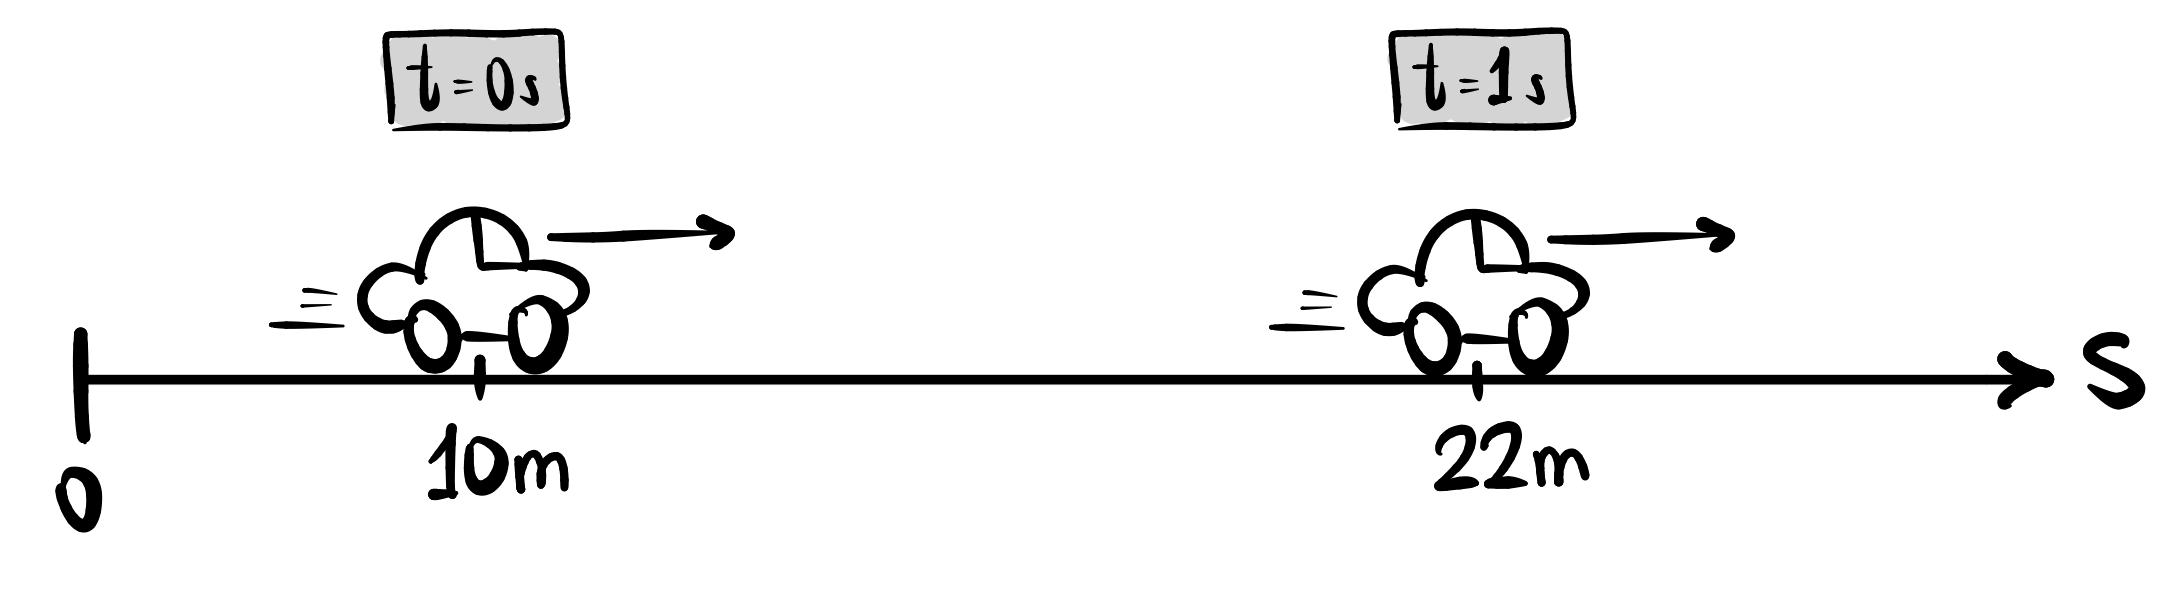
\includegraphics[scale=0.12]{imagensmecanica/mudvsdeltas1.jpeg}
    \caption{Carro em MU em um movimento progressivo.}
    \label{fig_mec_dvsdeltas1}
\end{figure}

A distância é igual ao comprimento da trajetória descrita pelo corpo em movimento. Em um movimento no qual não há inversão no seu sentido, é possível definir a distância como sendo o módulo do deslocamento, ou seja:
$$ d = |\Delta s|.$$

Neste caso, teríamos que $d=|12|=12$m, de modo que a velocidade, usando a Equação \eqref{mecanica_eq_distanciamu}, é dada por:

$$ v=\dfrac{d}{t}=\dfrac{12\text{m}}{1\text{s}}=12 \text{m/s.}$$

Considere agora a situação da Figura \ref{fig_mec_dvsdeltas2}, que é basicamente a mesma, porém de um carro que executa um movimento retrógrado, isto é, ele retrocede no eixo das posições. Calculando seu deslocamento, teríamos $\Delta s = 10-22=-12$m. Munidos disso, podemos calcular sua velocidade usando a Equação \eqref{mecanica_eq_velocidademedia}:

$$ v=\dfrac{\Delta s}{\Delta t}=\dfrac{-12\text{m}}{1\text{s}}=-12 \text{m/s.}$$



\begin{figure}[h]
    \centering
    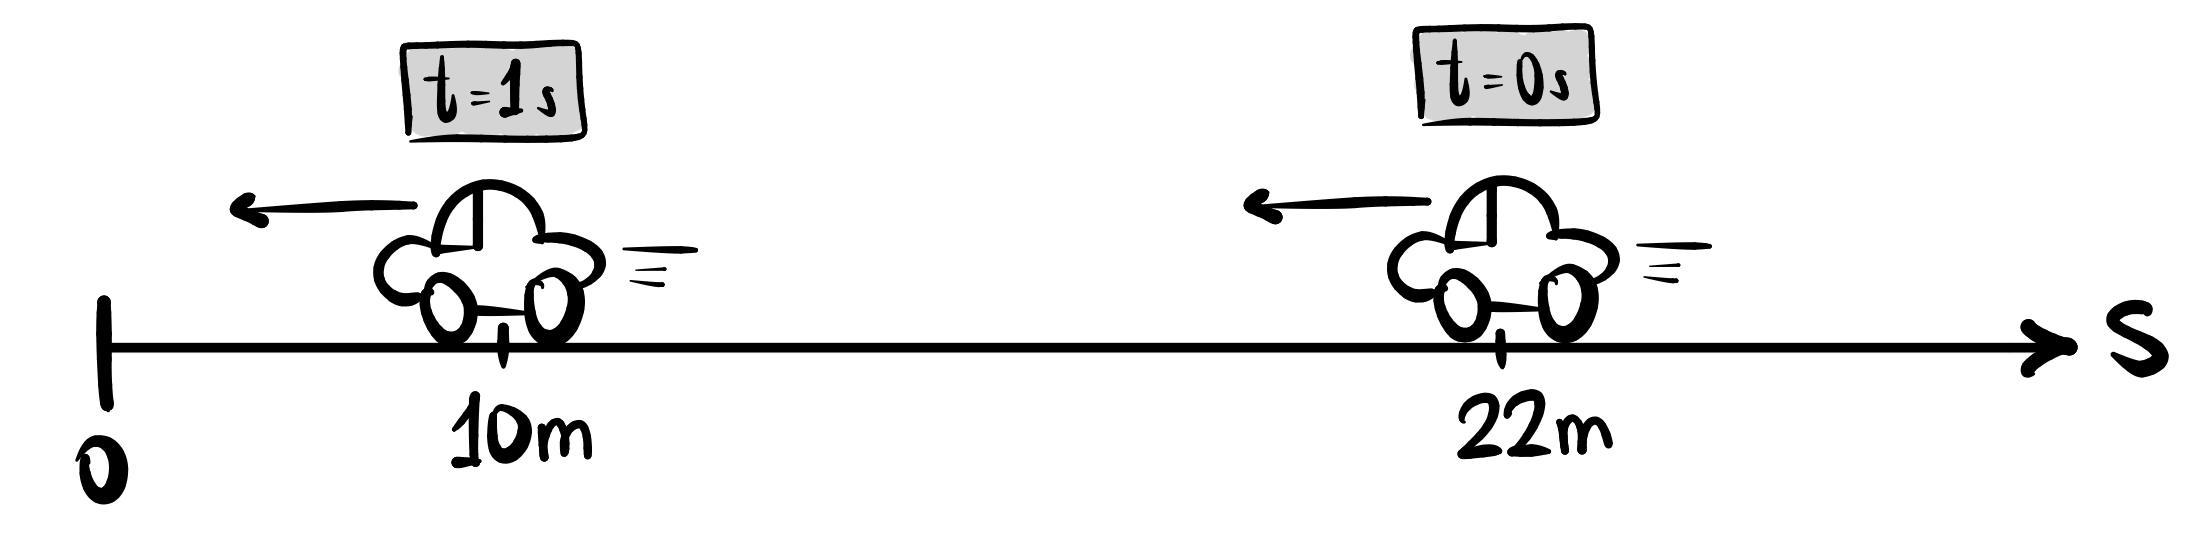
\includegraphics[scale=0.12]{imagensmecanica/mudvsdeltas12.jpeg}
    \caption{Carro em MU em um movimento retrógrado.}
    \label{fig_mec_dvsdeltas2}
\end{figure}


Ou seja, temos um carro que se move com a mesma \textit{rapidez} -- isto é, ele se desloca de 12m a cada 1s -- porém no sentido contrário ao que adotamos como o positivo -- é isso que o sinal negativo da velocidade significa.

Contudo, se fôssemos calcular a distância que o carro percorreu, teríamos que tal valor é $d=|\Delta s| = |-12|=12$m, o que não é de se estranhar: nos dois casos o carro percorreu uma distância de 12 metros. A distância não pode ser um número negativo, haja vista que ela mede um comprimento. Se eu me movo 12 metros para a direita ou para a esquerda a distância que percorri é a mesma nos dois casos: 12 metros.

Dito isso, se fôssemos agora calcular o valor da velocidade do carro usando a Equação \eqref{mecanica_eq_distanciamu}, teríamos:

$$ v = \dfrac{d}{t}=\dfrac{12\text{m}}{1\text{s}}=12 \text{m/s,}$$

\noindent e agora as coisas não concordam mais. O que aconteceu? Calculando a velocidade usando a ideia de deslocamento chegamos em $-12$ m/s, enquanto que usando a ideia de distância, chegamos em $12$ m/s.

Perceba que, na verdade, os resultados não são tão diferentes assim. O valor da velocidade -- a rapidez com que o corpo se move -- é o mesmo nos dois casos, eles só diferem por um sinal. Isso ocorre porque o conceito de velocidade usado nas Equações \eqref{mecanica_eq_velocidademedia} e \eqref{mecanica_eq_distanciamu} não é lá exatamente o mesmo. Veja bem: se a distância nunca pode ser negativa, uma vez que ela é um comprimento -- e foi inclusive definida neste contexto como sendo o módulo do deslocamento, o que é sempre positivo -- a velocidade, se computada por meio de $v=\sfrac{d}{t}$, jamais fornecerá um valor negativo. Nesse sentido, quando olhamos para a equação $d=vt,$ a velocidade que entra ali será sempre positiva -- ela estará medindo, na verdade, a rapidez absoluta com que o corpo se move. Usar a equação $d=vt$ sequer pressupõe que seja adotado um referencial: tanto faz para onde é o sentido positivo convencionado, porque aqui, neste caso, pegaremos sempre o módulo do deslocamento, que é sempre positivo, e isso fará com que a velocidade nunca fique negativa.

Assim, ao usarmos $d=vt$, a velocidade nunca entrará com sinal negativo -- essa é a forma como tal equação foi construída. Logo, para resolver problemas, teremos que avaliar as características geométricas e espaciais deles -- isso porque, como mostram as Figuras \ref{fig_mec_dvsdeltas1} e \ref{fig_mec_dvsdeltas2}, a velocidade, nesse critério, seria de $12$ m/s para os dois casos; ou seja, ela não diferencia quem se move para um lado ou para o outro -- ela olha só a \textit{rapidez com que o corpo se move.}

Já quando usamos a velocidade por meio de $v=\sfrac{\Delta s}{\Delta t},$ o valor absoluto será sempre o mesmo daquele calculado por meio de $v=\sfrac{d}{t},$ podendo diferir deste apenas de um sinal\footnote{Isso vale apenas para o Movimento Uniforme, que é o contexto no qual estamos.}, uma vez que o deslocamento pode ser positivo ou negativo. Assim, a velocidade, quando computada por meio da Equação \eqref{mecanica_eq_velocidademedia}, pressuporá, sempre, a adoção de uma convenção acerca de qual é o sentido positivo, e a velocidade poderá ser positiva ou negativa, a depender se ela aponta no mesmo sentido ou em sentido contrário ao que escolhemos como sendo o positivo.

Nesse sentido, podemos entender a velocidade média definida como sendo a razão entre deslocamento e tempo como um conceito mais completo do que aquele em que a velocidade pudesse ser computada como sendo a distância pelo tempo. Ele é mais completo no sentido que consegue capturar -- através do sinal -- corpos que se movem com a mesma rapidez porém em sentidos diferentes. Quando falamos de distância é impossível capturarmos tal informação, haja vista que se mover 12 metros para a direita ou para a esquerda dá na mesma. 

Como dito no início, essa se tratava de uma conversa um pouco abstrata. A resolução do próximo exemplo deixará mais clara a diferença que pontuamos aqui. Sugiro ao leitor que compare a solução do próximo exemplo com aquela que fizemos deste mesmo problema ao discutir a Equação \eqref{mecanica_eq_distanciamu}.

%Exemplo resolvido

\vspace{0.3cm}

\begin{exemplo}[Nível I]\label{exemplo_funcaohorariaposicaomu01}


Um carro se move com velocidade constante de 20 m/s ao longo de uma rodovia, enquanto outro se move com velocidade constante de 30 m/s, em sentido oposto, ao longo da mesma rodovia.

Se os carros inicialmente estão separados por uma distância de 1.2 km, após quanto tempo eles irão passar um pelo outro?


\resolucao

Sim, este é o mesmo exercício que fizemos anteriormente. Daremos, agora, uma terceira solução para ele. 

\medskip

Para resolver o problema usando a função horária da posição é preciso, antes de tudo, definir uma origem e uma orientação a fim de que as posições possam ser marcadas. Considere a Figura \ref{fig_mec_sorveteexemplo011}, que mostra uma escolha feita: consideramos a origem como sendo a posição inicial do carro $A$ e, consequentemente, a posição inicial de $B$ será $s_0=1200$m, uma vez que os carros estão inicialmente separados por tal distância e o eixo está orientado para direita.

{
\centering
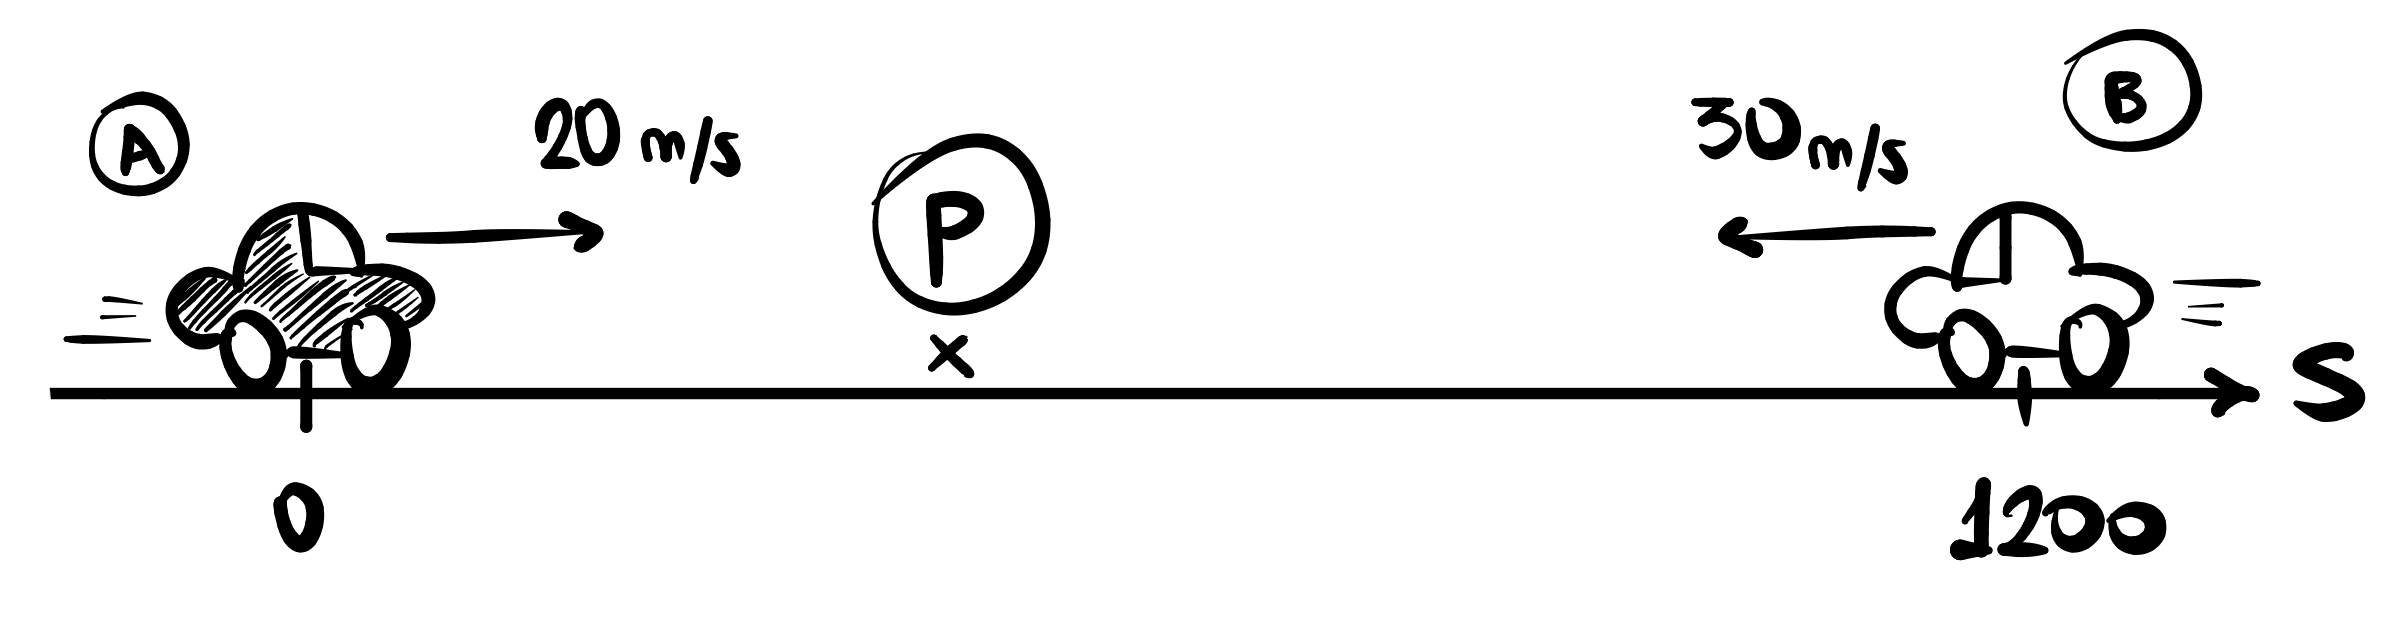
\includegraphics[width=0.6\linewidth]{imagensmecanica/sorveteexemplo011.jpeg}
\captionof{figure}{Referencial orientado para direita com origem na posição inicial do carro A.}
\label{fig_mec_sorveteexemplo011}
} 
\vspace{0.3cm}

Em tal referencial as funções de posição dos carros são:

\begin{enumerate}
    \item [(A)] $s_A= s_0+vt = \cancelto{0}{s_0}+20t \implies \boxed{s_A=20t.}$

    \item [(B)] $s_B= s_0+vt = 1200-30t \implies \boxed{s_B=1200-30t.}$
\end{enumerate}

Ora, dizer que os carros vão passar um pelo outro significa que, em um certo instante $t$, as suas posições irão coincidir -- na posição representada pelo ponto $P$ na figura. Ou seja, os carros se encontram quando $s_A=s_B:$

$$ 20t = 1200-30t \implies 50t = 1200 \implies \boxed{t = 24 \text{ segundos.}}$$

Naturalmente, obtivemos a resposta que já esperávamos. Note que tal resposta independe, é claro, do referencial adotado: o tempo, na mecânica clássica, é absoluto. Assim, se leva 24 segundos para que algo aconteça em um referencial, levará 24 segundos para que isso aconteça em qualquer outra referencial.  


\medskip

Considere, por exemplo, a origem e orientação adotadas no referencial da Figura \ref{fig_mec_sorveteexemplo012}: neste caso alteramos a origem, que agora está a 100 metros para a esquerda de $A.$ Assim, sendo a distância entre os carros inicialmente de $1200$m, a posição do carro $B$ deve ser $100+1200=1300$m, como mostra a figura.

\vspace{0.3cm}
{
\centering
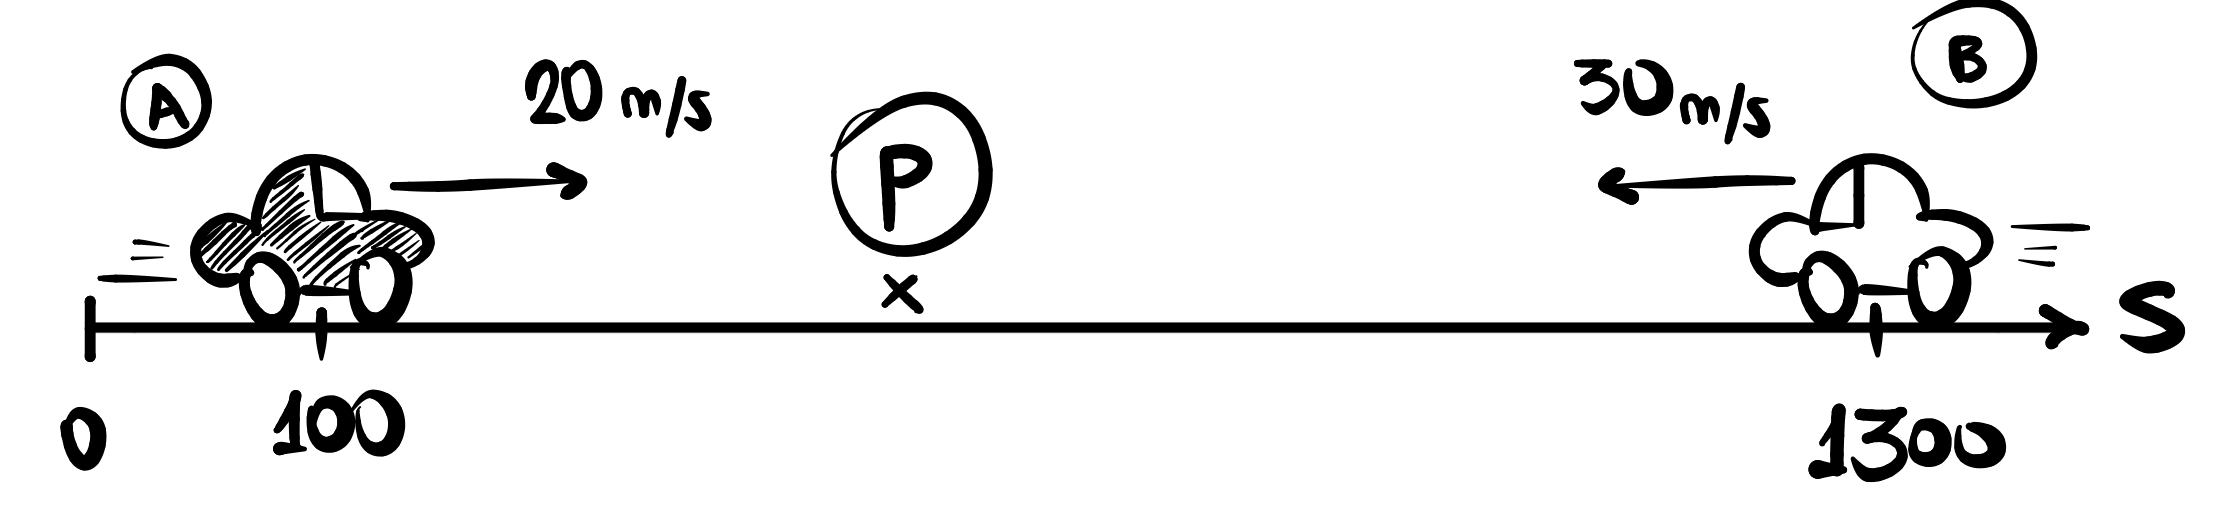
\includegraphics[width=0.6\linewidth]{imagensmecanica/sorveteexemplo012.jpeg}
\captionof{figure}{Referencial orientado para direita com origem arbitrária.}
\label{fig_mec_sorveteexemplo012}
} 
\vspace{0.3cm}

Em tal referencial as funções de posição dos carros são:

\begin{enumerate}
    \item [(A)] $s_A= s_0+vt = 100+20t \implies \boxed{s_A=100+20t.}$

    \item [(B)] $s_B= s_0+vt = 1300-30t \implies \boxed{s_B=1300-30t.}$
\end{enumerate}

Para que eles se encontrem é preciso que $s_A=s_B:$

$$ 100+20t = 1300 - 30t \implies 50t = 1200 \implies \boxed{t = 24 \text{ segundos.}}$$

Logo, adotando uma origem diferente, as funções horárias da posição mudam, mas a nossa resposta final segue sendo a mesma, como deve ser. \\


\medskip

Considere agora um terceiro referencial adotado na Figura \ref{fig_mec_sorveteexemplo013}, que em mudamos não apenas a origem mas também a orientação (note, porém, que as posições iniciais dos carros, por mais arbitrárias que sejam, precisam satisfazer a condição de que suas diferenças sejam de 1200 metros, uma vez que essa é a situação inicial do problema físico.)

\vspace{0.3cm}
{
\centering
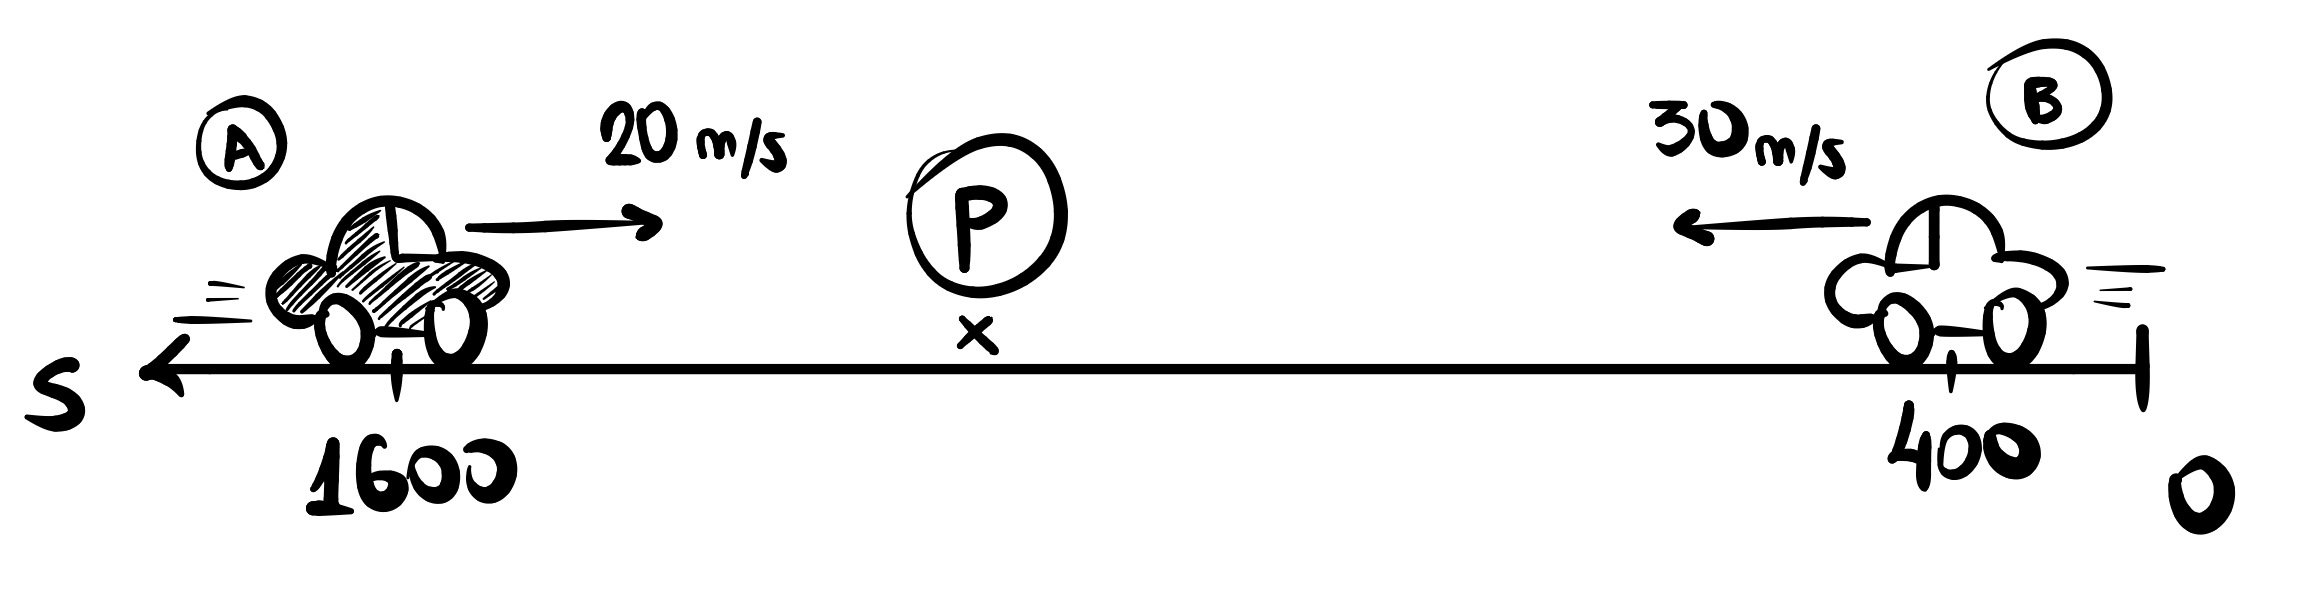
\includegraphics[width=0.6\linewidth]{imagensmecanica/sorveteexemplo013.jpeg}
\captionof{figure}{Referencial orientado para esquerda com origem arbitrária.}
\label{fig_mec_sorveteexemplo013}
} 
\vspace{0.3cm}

Em tal referencial as velocidades para a direita serão negativas, e as velocidades para a esquerda se tornam positivas, de modo que as funções de posição dos carros são:

\begin{enumerate}
    \item [(A)] $s_A= s_0+vt = 1600-20t \implies \boxed{s_A=1600-20t.}$

    \item [(B)] $s_B= s_0+vt = 400+30t \implies \boxed{s_B=400+30t.}$
\end{enumerate}

Para que eles se encontrem é preciso que $s_A=s_B:$

$$ 1600-20t = 400+30t \implies 50t = 1600 - 400 = 1200 \implies \boxed{t = 24 \text{ segundos.}}$$

Ou seja, para computar o intervalo de tempo entre dois eventos é indiferente o referencial adotado -- bastando, para tanto, se atentar aos sinais da velocidade para as diferentes orientações adotadas. Em sistemas de coordenadas (referenciais) distintos as posições iniciais e finais podem ser diferentes, os sinais da velocidade podem mudar, as equações de posição mudam, mas o intervalo de tempo para que algo aconteça é sempre o mesmo.\footnote{A posição no espaço na qual os carros se encontram também é a mesma: a colisão ocorre sempre no mesmo lugar geométrico do espaço. Tal lugar, contudo, receberá atribuições numéricas diferentes a depender da escolha da origem. Como o leitor pode verificar, nos três referenciais escolhidos, as posições de encontro serão, respectivamente, em $s_1=480$m, $s_2=580$m e $s_3=1120$m. O encontro, apesar de ocorrer no mesmo lugar geométrico do espaço, recebe coordenadas diferentes devido às diferentes escolhas de origem e orientação.}
 
 

\end{exemplo}

\vspace{0.3cm}






\begin{exemplo}[Nível II]\label{exemplo_funcaohorariaposicaomu02}


Considere três carros $A, B$ e $C,$ que se movem, respectivamente, com as velocidades $v_A=60$ m/s, $v_B=20$ m/s e $v_C=40$ m/s. O carro $B$ se encontra, inicialmente, $120$ metros a frente do carro $A$; e o carro $C$, por sua vez, $120$ metros a frente do carro $B.$ \\

A partir de tal configuração, após quanto tempo o carro $A$ estará entre $B$ e $C,$ exatamente no meio do caminho entre os dois?


\resolucao

Considere o referencial adotado na Figura \ref{fig_mec_funcaoposicaoexemplo011}, com a origem na posição inicial de $A.$ Em tal referencial as equações de posição são:

\begin{enumerate}
    \item [(A)] $s_A= \cancelto{0}{s_0}+vt \implies s_A=60t.$

    \item [(B)] $s_B= s_0+vt \implies s_B=120+20t.$

    \item [(C)] $s_C= s_0+vt \implies s_C=240+40t.$
\end{enumerate}

{
\centering
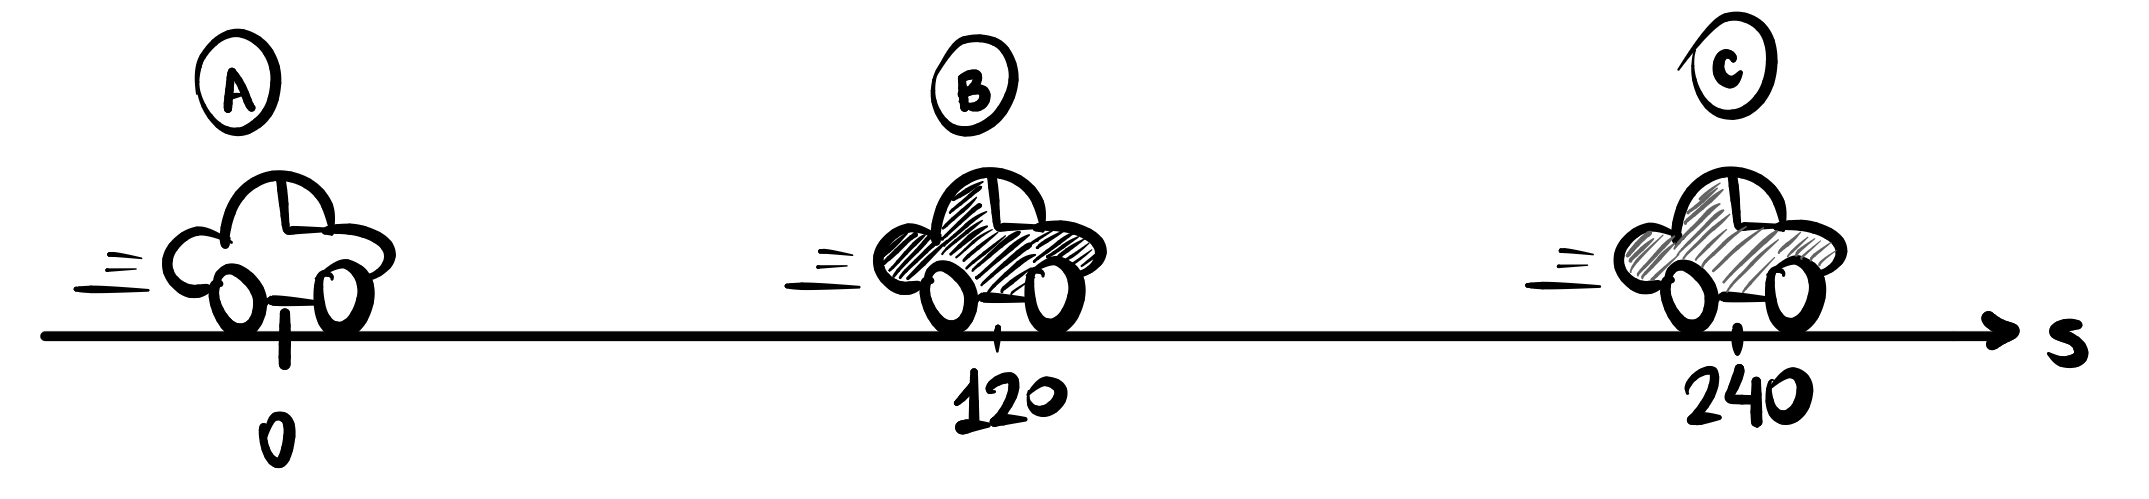
\includegraphics[width=0.6\linewidth]{imagensmecanica/funcaoposicaoexemplo011.jpeg}
\captionof{figure}{Representação do problema com escolha de referencial.}
\label{fig_mec_funcaoposicaoexemplo011}
} 
\vspace{0.3cm}

A configuração buscada é aquela da Figura \ref{fig_mec_funcaoposicaoexemplo012}, na qual, para que $A$ esteja exatamente no meio do caminho entre $B$ e $C$, as distâncias destacadas devem ser iguais, isto é:

$$ s_A-s_B = s_C-s_A,$$
o que nos leva a

$$ s_A = \dfrac{s_B+s_C}{2},$$
ou seja, a posição de $A$ será exatamente a média aritmética das posições de $B$ e $C$ -- ele estará exatamente no meio do caminho.

\vspace{0.3cm}
{
\centering
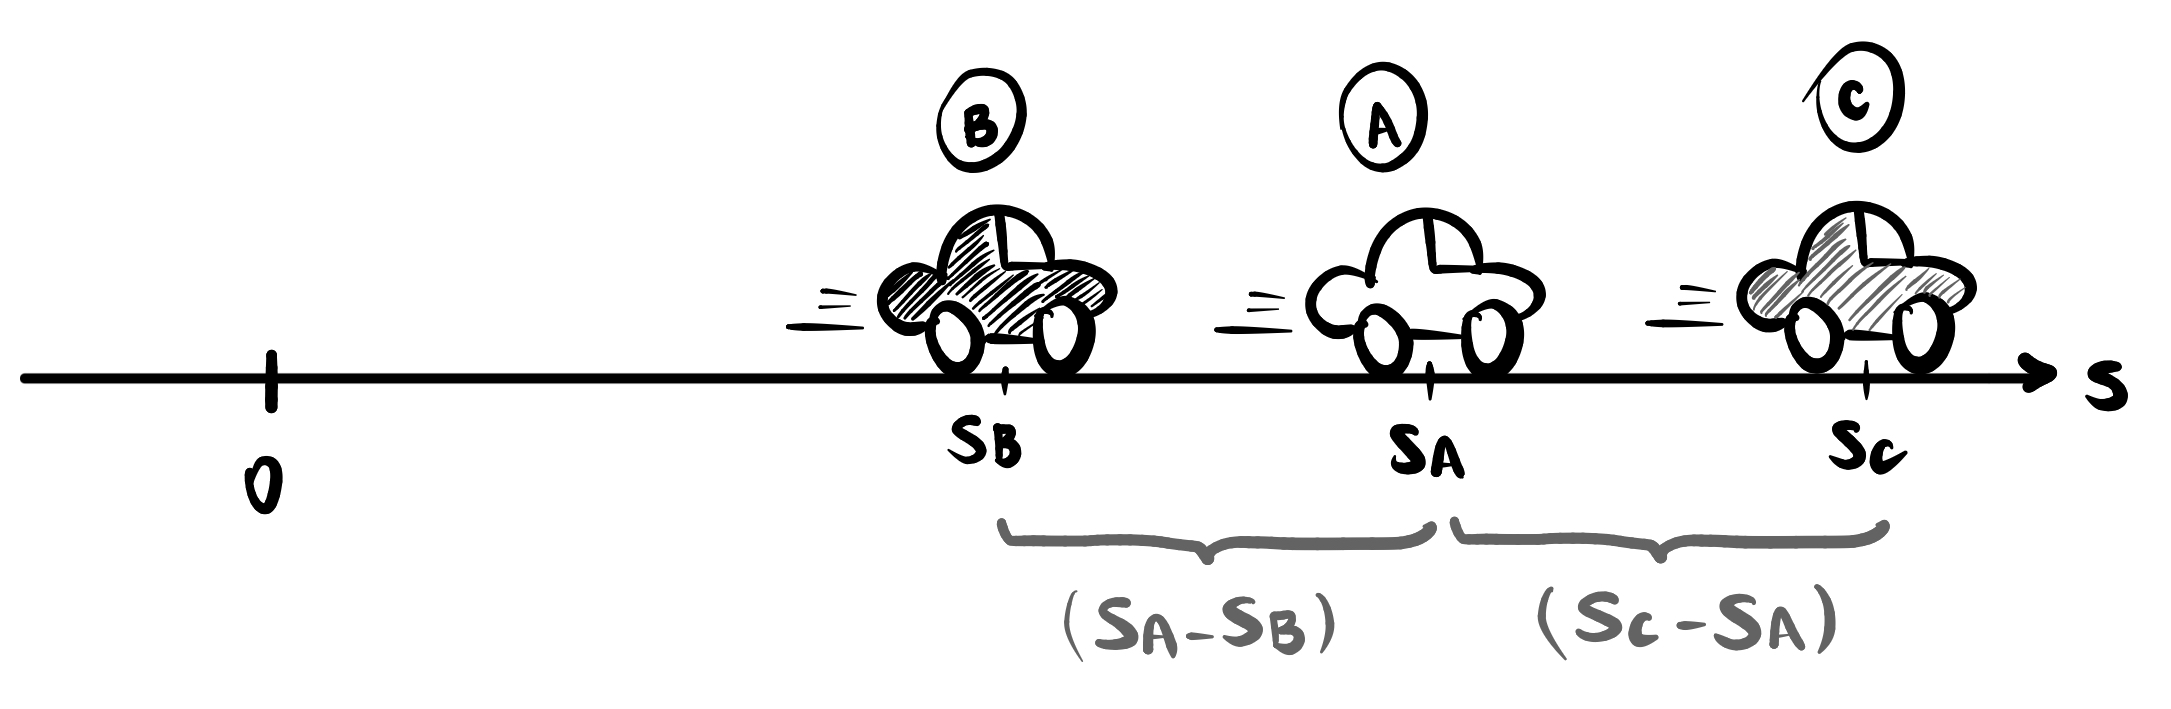
\includegraphics[width=0.6\linewidth]{imagensmecanica/funcaoposicaoexemplo012.jpeg}
\captionof{figure}{Carro $A$ exatamente a meia distância entre os carros $B$ e $C.$}
\label{fig_mec_funcaoposicaoexemplo012}
} 
\vspace{0.3cm}
Usando as equações de posições construídas, chegamos em

$$ s_A = \dfrac{s_B+s_C}{2} \implies 60t = \dfrac{360+60t}{2} \implies \boxed{t = 6 \text{ segundos.}}$$
 
 

\end{exemplo}

\vspace{0.3cm}







\begin{exemplo}[Nível III (ITA - 1985)]\label{exemplo_funcaohorariaposicaomu03}


Um ônibus parte do Rio de Janeiro para Curitiba às $7$ horas da manhã; às $12$ horas parte outro ônibus de Curitiba para o Rio. Percorrem os $720$ km entre as duas cidades em $12$ horas. A hora e a distância do Rio de Janeiro em que os ônibus se encontram, são, respectivamente:
\begin{enumerate}
\item[(a)] $08$h$30$ min e $220$ km.
\item[(b)] $15$h$30$ min e $220$ km.
\item[(c)] $08$h$30$ min e $510$ km.
\item[(d)] $15$h$30$ min e $510$ km.
\item[(e)] $15$h$30$ min e $498$ km.
\end{enumerate}


\resolucao


 Assumindo que os ônibus se movem com velocidade constante, seja $A$ e $B$ os pontos que representam o Rio de Janeiro e Curitiba, respectivamente. Considere um eixo de posições com origem em $A$ e orientado de $A$ para $B$. Logo, nesse sistema, a função horária da posição do ônibus que sai do Rio para Curitiba -- chamemo-lo de ônibus $1$ -- é

$$ s_1 = \cancelto{0}{s_0}+vt \implies s_1(t)=60t,$$

\noindent em que  velocidade de cada ônibus, sendo constante, é dada por

$$ v= \dfrac{d}{\Delta t} = \dfrac{720 \text{ km}}{12 \text{ h}}= 60 \text{ km/h.}$$

A função horária da posição do ônibus que sai de Curitiba para o Rio -- chamemo-lo de ônibus $2$ -- é

$$ s_2 = s_0 + vt' \implies s_2(t)=720-60(t-5).$$

Note que os cronômetros $t$ e $t'$ que cronometram os movimentos completos dos ônibus $1$ e $2$ são diferentes, uma vez que este começa a se mover apenas $5$ horas após o início do movimento daquele. Logo, para ajustar isso, o tempo do segundo ônibus deve ser $t'=t-5$. Perceba que isso está de acordo, porque em $t=5$ h (tempo cronometrado a partir do início do movimento do ônibus $1$) o ônibus $2$ estará iniciando o seu movimento, isto é, estará em $t'=t-5=0.$

Sendo assim, os ônibus se encontram quando $s_1(t)=s_2(t),$ ou seja:

$$ 60t = 720-60(t-5) \implies \boxed{t=8.5 \text{ h},}$$

\noindent e, como o tempo $t$ foi medido a partir do início do movimento do ônibus $1$, isto é, $t=0$ era às 07h00, então o horário do encontro ocorre em $07\text{h}00+08\text{h}30=15\text{h}30.$

A posição do encontro ocorre em

$$ s_1(t) = 60t =  \boxed{510 \text{ km}.}$$

Sendo a origem do sistema de coordenadas no Rio de Janeiro, a distância do ponto de encontro ao Rio é dada exatamente por $510$ km.
 

\end{exemplo}

\vspace{0.3cm}















\newpage




\section{Movimento Uniformemente Variado}

Tal movimento é \textbf{definido}\footnote{Ou seja, estamos criando vocabulário: dando um nome específico a um tipo específico de movimento.} como sendo aquele no qual o \textbf{valor da aceleração do objeto é constante}. Ou seja, como mostra a Figura \ref{fig_mec_muv}, a velocidade irá variar de quantidades iguais em iguais intervalos de tempo. Em tal exemplo, para quaisquer intervalos de tempo que o leitor escolher, o valor da aceleração será sempre o mesmo. Façamos alguns cálculos, a fim de tornar isso claro. Considerando o intervalo de tempo de $0$s a $1$s, teríamos:

$$ a_{1} = \dfrac{\Delta v}{\Delta t} = \dfrac{4-2}{1-0} = \dfrac{2 \text{m/s}}{1\text{s}} = 2 \text{m/s}^2.$$

Considerando agora intervalo de tempo de $1$s a $2$s, teríamos:

$$ a_{2} = \dfrac{\Delta v}{\Delta t} = \dfrac{6-4}{2-1} = \dfrac{2 \text{m/s}}{1\text{s}} = 2 \text{m/s}^2.$$

Se avaliarmos agora no intervalo de tempo total do movimento, de $0$s a $3$s, teríamos:

$$ a_{3} = \dfrac{\Delta v}{\Delta t} = \dfrac{8-2}{3-0} = \dfrac{6 \text{m/s}}{3\text{s}} = 2 \text{m/s}^2,$$

\noindent ou seja, o padrão de variação da velocidade é claro: ela muda sempre a uma mesma taxa, qualquer que seja o intervalo de tempo em que avaliarmos o movimento. Isso é o que define o movimento uniformemente variado.

\begin{figure}[h]
    \centering
    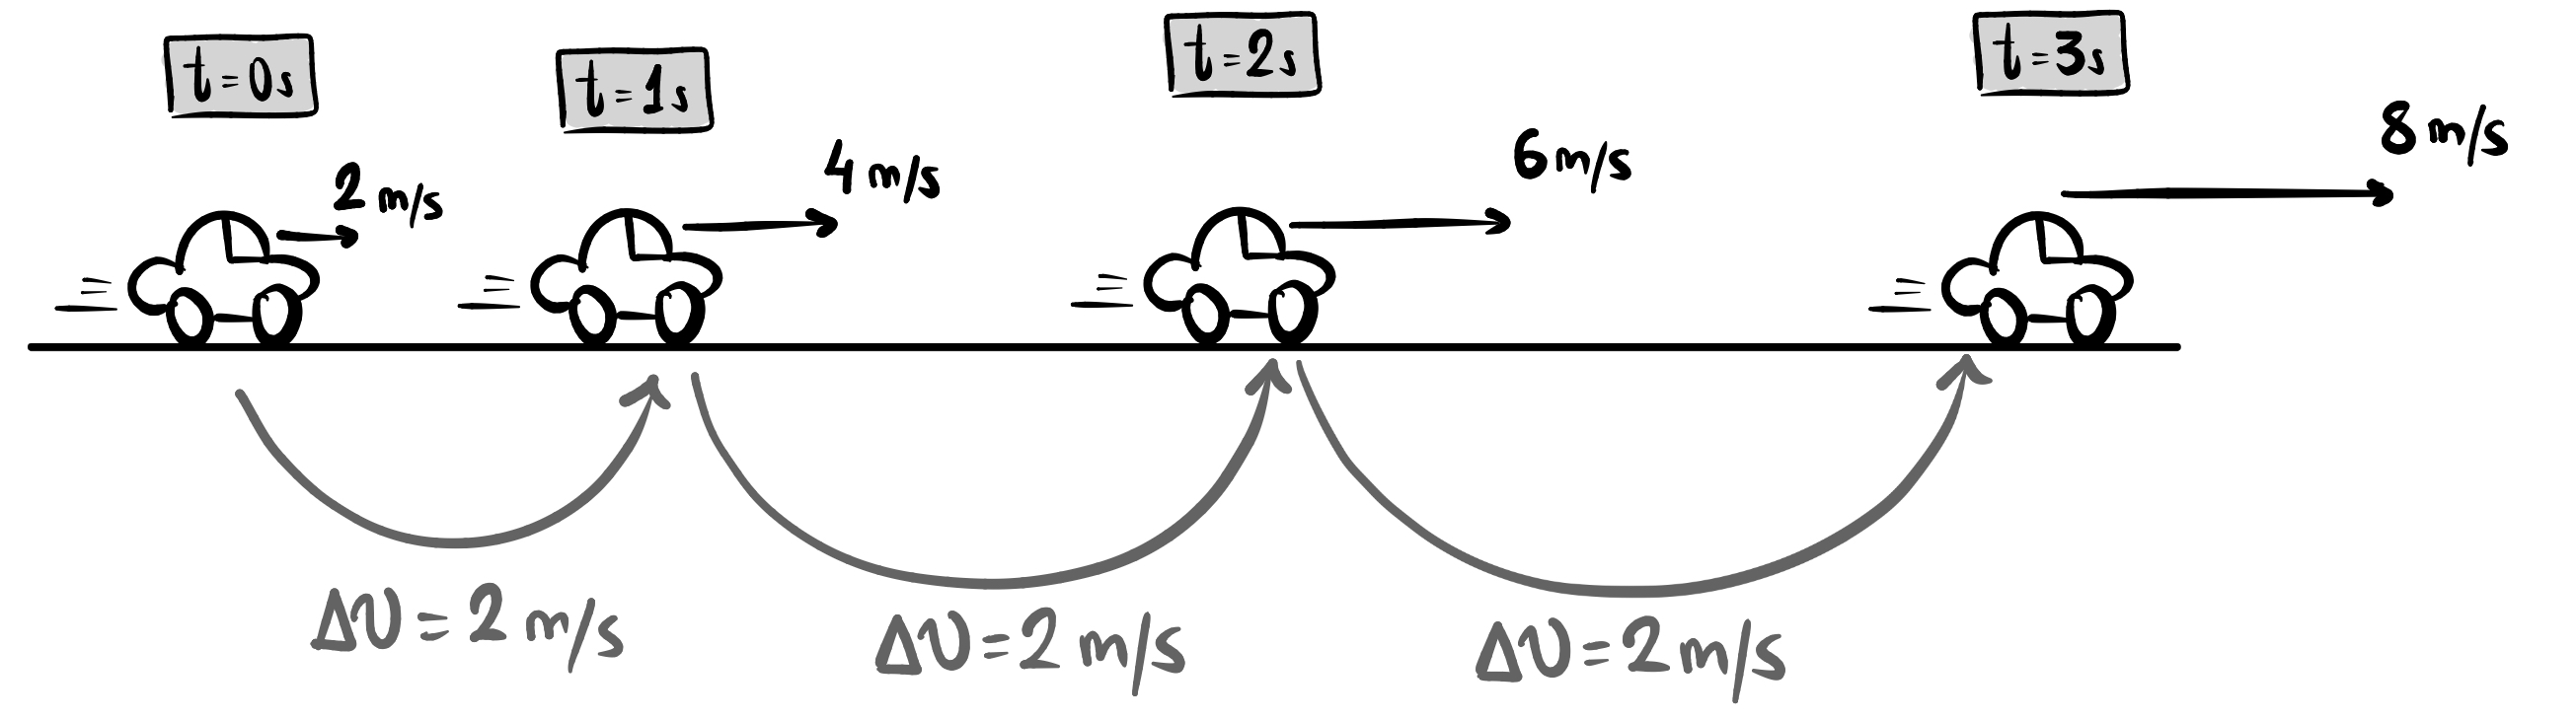
\includegraphics[scale=0.15]{imagensmecanica/muvexemplo.jpeg}
    \caption{O movimento com aceleração constante}
    \label{fig_mec_muv}
\end{figure}

Contudo, é importante que fique claro também o que \textbf{não é} um movimento uniformemente variado, e a Figura \ref{fig_mec_muvcontraexemplo} ilustra um exemplo. Perceba que trata-se um movimento acelerado -- isto é, no qual a velocidade varia -- porém a forma como a velocidade varia não é a mesma o tempo inteiro. Note que, se fôssemos calcular o valor da aceleração do corpo, não teríamos um único valor. 


\begin{figure}[h]
    \centering
    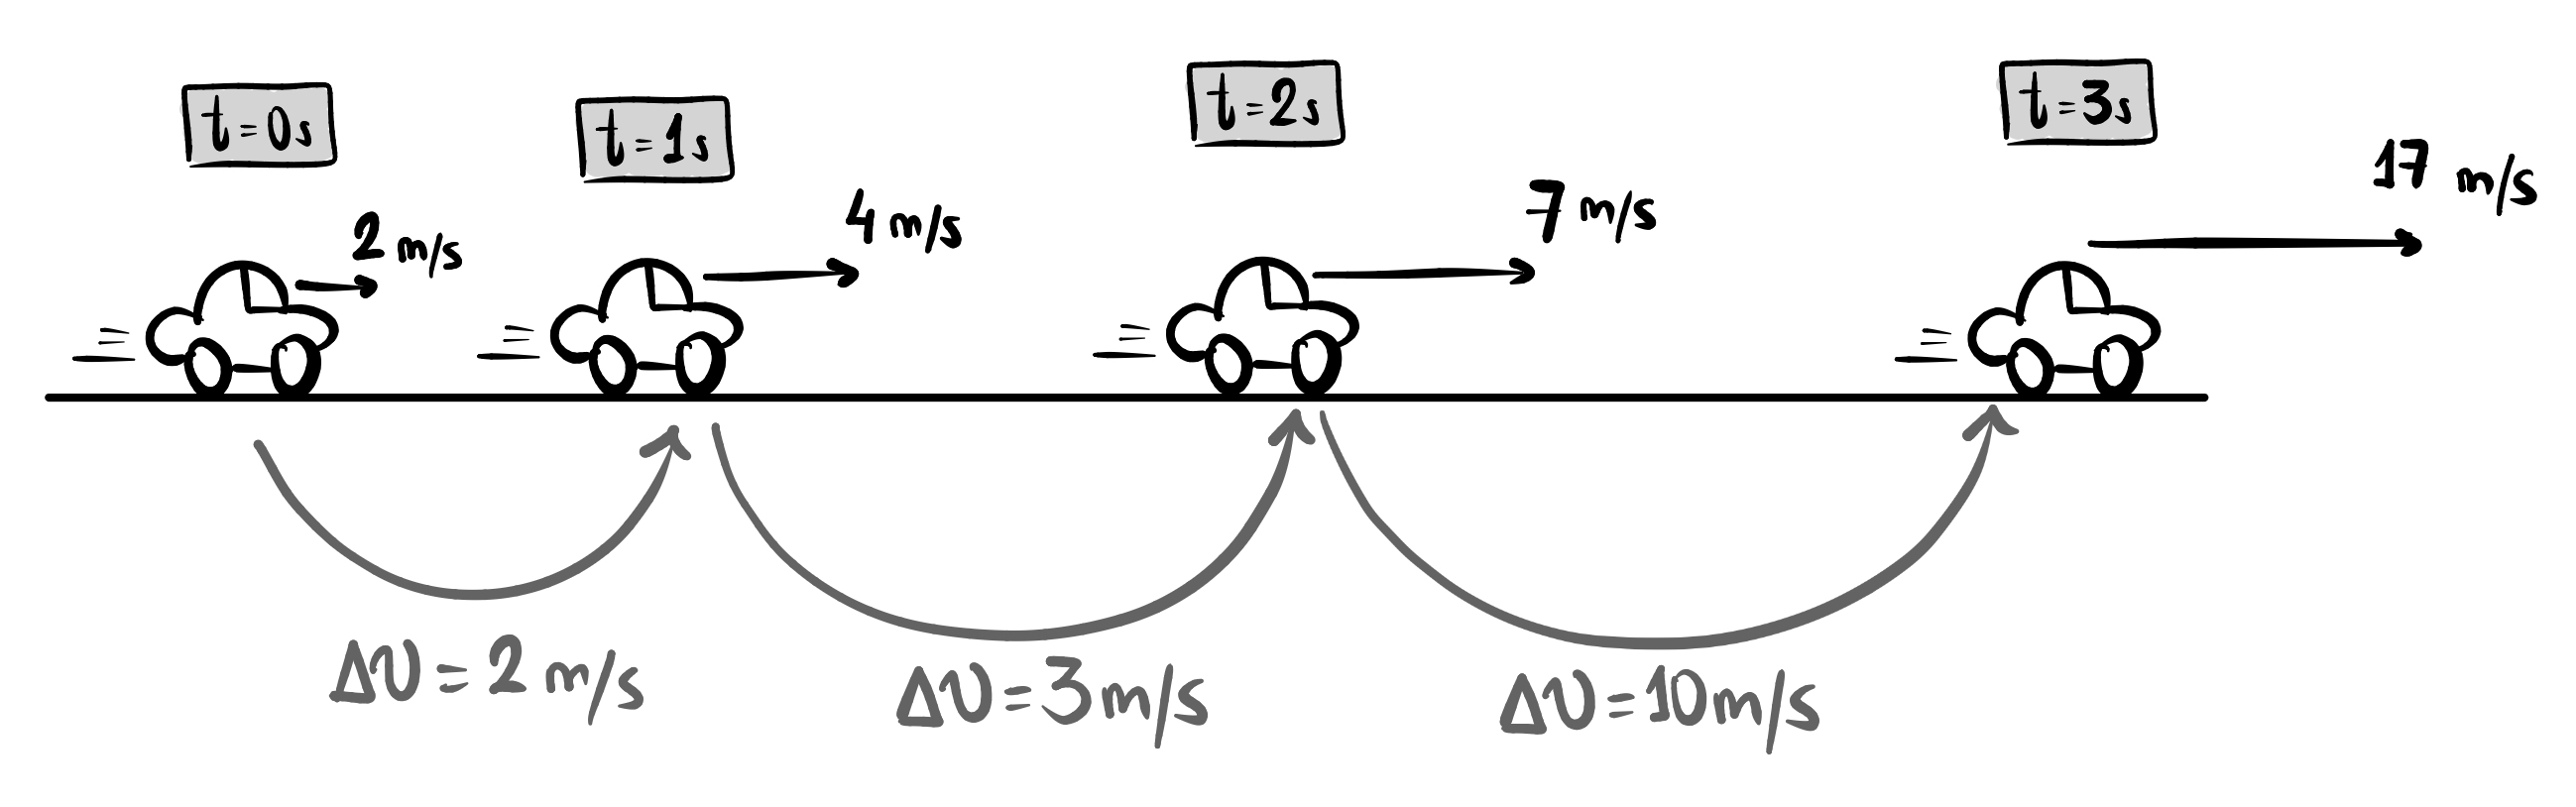
\includegraphics[scale=0.15]{imagensmecanica/muvcontraexemplo.jpeg}
    \caption{O movimento acelerado que não é uniformemente variado.}
    \label{fig_mec_muvcontraexemplo}
\end{figure}


Considerando o intervalo de tempo de $0$s a $1$s, teríamos:

$$ a_{1} = \dfrac{\Delta v}{\Delta t} = \dfrac{4-2}{1-0} = \dfrac{2 \text{m/s}}{1\text{s}} = 2 \text{m/s}^2.$$

Agora, avaliando no intervalo de tempo de $1$s a $2$s, teríamos:

$$ a_{2} = \dfrac{\Delta v}{\Delta t} = \dfrac{7-4}{2-1} = \dfrac{3 \text{m/s}}{1\text{s}} = 3 \text{m/s}^2.$$

E, se avaliássemos no intervalo de tempo total,  de $0$s a $3$s, teríamos:

$$ a_{3} = \dfrac{\Delta v}{\Delta t} = \dfrac{17-2}{3-0} = \dfrac{15 \text{m/s}}{3\text{s}} = 5 \text{m/s}^2.$$


Note que, neste caso, a velocidade varia, porém não de uma forma constante -- o incremento da velocidade para um mesmo intervalo de tempo é cada hora um, de modo que tal movimento é acelerado, porém não é uniformemente variado.

Agora que está claro do que se trata um movimento uniformemente variado, podemos analisar as equações que o descrevem.








\begin{secnivel}[Função Horária da Velocidade no MUV]
{I}{Função Horária da Velocidade do Movimento Uniformemente Variado}
 

  \eqLdois{dem}{mecanica_eq_muvfuncaovelocidade}{v=v_0+at}
  
\end{secnivel}







\secgfe{De onde vem}

Observe a Figura \ref{fig_mec_funcaovelocidade02}, na qual temos um objeto que se move em um Movimento Uniformemente Variado (MUV) com velocidade inicial $v_0$ no instante inicial $t_0=0$s, alcançando uma velocidade $v$ no instante $t$. Queremos uma equação em que, sabendo o valor da aceleração $a$ do objeto e sua velocidade inicial $v_0$, possamos encontrar, para qualquer instante de tempo futuro $t$, o valor da sua velocidade $v$ naquele instante.

\begin{figure}[h]
    \centering
    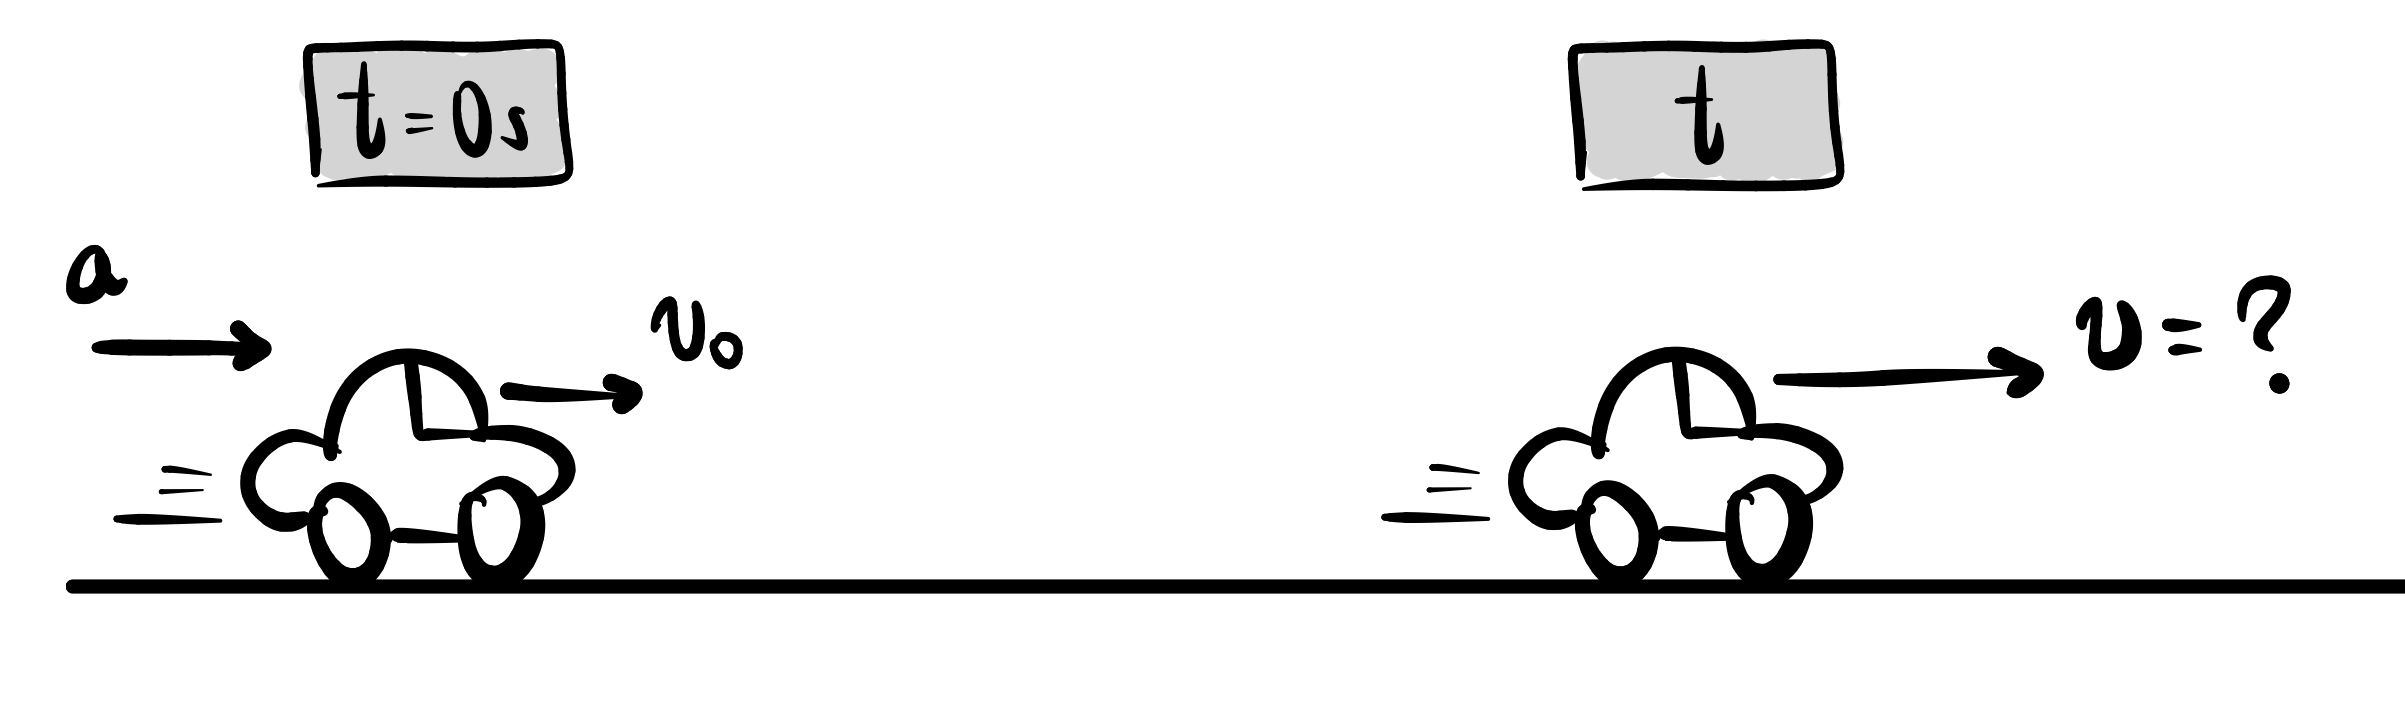
\includegraphics[scale=0.12]{imagensmecanica/muvfuncaovelocidade02.jpeg}
        \caption{A construção da função horária da velocidade para o MUV.}
    \label{fig_mec_funcaovelocidade02}
\end{figure}

A equação que vamos construir é uma consequência natural da definição de aceleração e da forma como definimos o MUV. Note que, pela Equação \eqref{mecanica_eq_aceleracaomedia}, temos que

$$ a_M = \dfrac{\Delta v}{\Delta t} =\dfrac{v-v_0}{t-0}, $$

\noindent contudo, sendo o movimento um MUV, a aceleração $a$ é constante o tempo inteiro, de modo que a aceleração média em qualquer intervalo de tempo será sempre igual a $a$, uma vez que a aceleração nunca muda. Assim, teremos

$$ a_M = a = \dfrac{v-v_0}{t-0} \implies \boxed{v = v_0 + at.} $$

Mais uma vez, vale destacar a finalidade de tal equação: de modo geral, conhecemos quem é a velocidade inicial $v_0$ de um certo objeto, qual é o valor de sua aceleração $a$ e, com tal equação, podemos descobrir o valor de sua velocidade $v$ para qualquer instante futuro de tempo $t$. Desse modo, tal equação é uma função do tempo, e poderíamos escrevê-la de modo a deixar isso explícito como

$$ v(t) = v_0+at,$$
ou seja, $v_0$ e $a$ são os coeficientes de tal função afim, $t$ é a sua variável e, para cada valor de $t$ a equação de retorna um valor de $v$ associado a ele: o valor da velocidade do móvel naquele instante específico. De modo mais concreto, considere um movimento acelerado em que a aceleração é $a=3$ m/s$^2$ e a velocidade inicial é $v_0=5$ m/s. Logo, a função horária da velocidade de tal movimento é

$$ v(t) = 5+3t.$$

Ou seja, com tal equação é possível saber o valor da velocidade $v$ do carro em $t=3$s, que seria de $14$ m/s; ou em  $t=25$s, que seria de $80$ m/s. De modo geral, tal equação fornece a velocidade do móvel para qualquer instante de tempo que se queira.



\secgfe{Onde é usada}

Usamos essa equação em diversos problemas de MUV nos quais estamos interessados em computar a velocidade do objeto que executa tal movimento. Considere, por exemplo, o contexto da Figura \ref{fig_mec_funcaovelocidade01}, no qual um carro executa um MUV. Como poderíamos proceder caso quiséssemos saber a sua velocidade no oitavo segundo do movimento?

\begin{figure}[h]
    \centering
    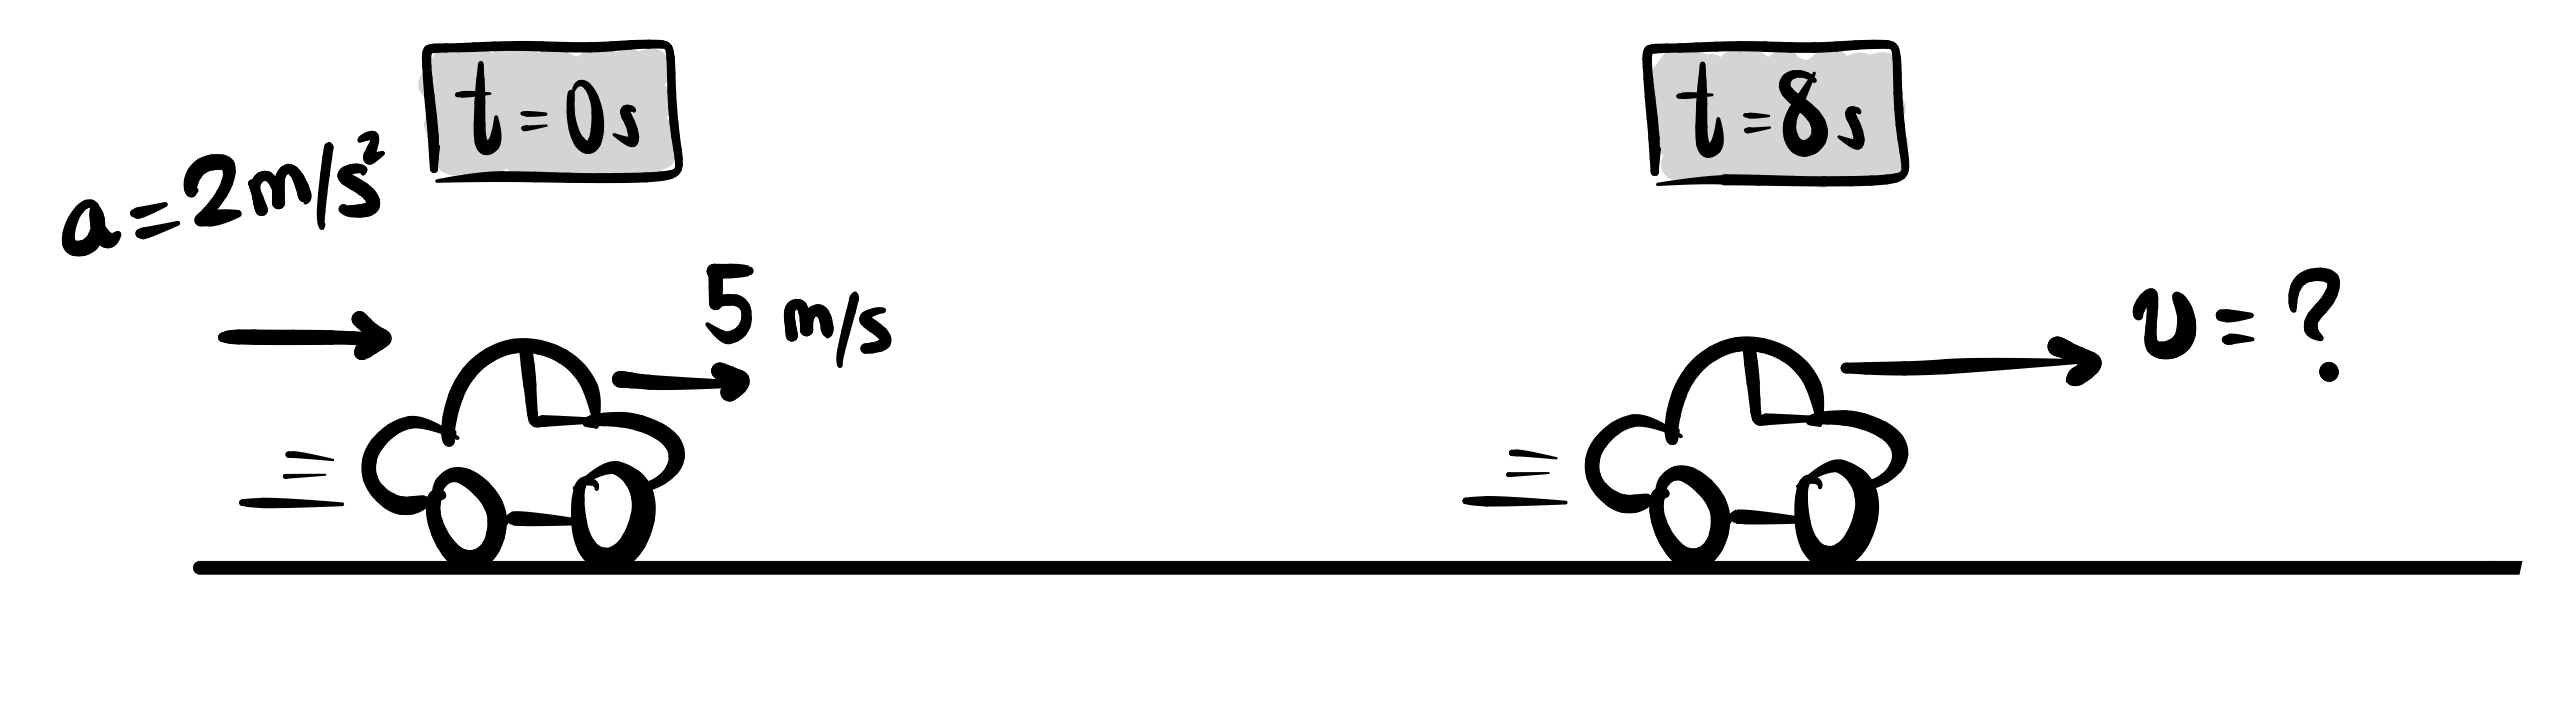
\includegraphics[scale=0.12]{imagensmecanica/muvfuncaovelocidade01.jpeg}
    \caption{Exemplo de um MUV.}
    \label{fig_mec_funcaovelocidade01}
\end{figure}

Ora, isso é justamente o que faz a função horária da velocidade:

$$v(t)=v_0+at \implies v(t) = 5 + 2t.$$

Munidos de tal equação, podemos descobrir o valor da velocidade do carro em qualquer instante. Em particular, para $t=8$s, teríamos

$$ v(8)=5+2\cdot 8= 21 \text{m/s}.$$


\secgfe{Erros comuns}

Os erros mais comuns no uso de tal equação consistem em:

\begin{itemize}
    \item [(i)] Confusão com o instante inicial.

    Note que, na própria demonstração da Equação \eqref{mecanica_eq_muvfuncaovelocidade}, definimos que em $t_0=0$s o valor da velocidade era $v_0.$ Logo, para usarmos corretamente tal equação neste formato, é preciso levar isso com rigor. Note, por exemplo, o MUV representado na Figura \ref{fig_mec_muvfuncaovelocidade04}. Está nítido que se trata de um MUV, no qual a aceleração vale $a=2$m/s$^2,$ como o leitor bem pode verificar. 
    
\begin{figure}[h]
    \centering
    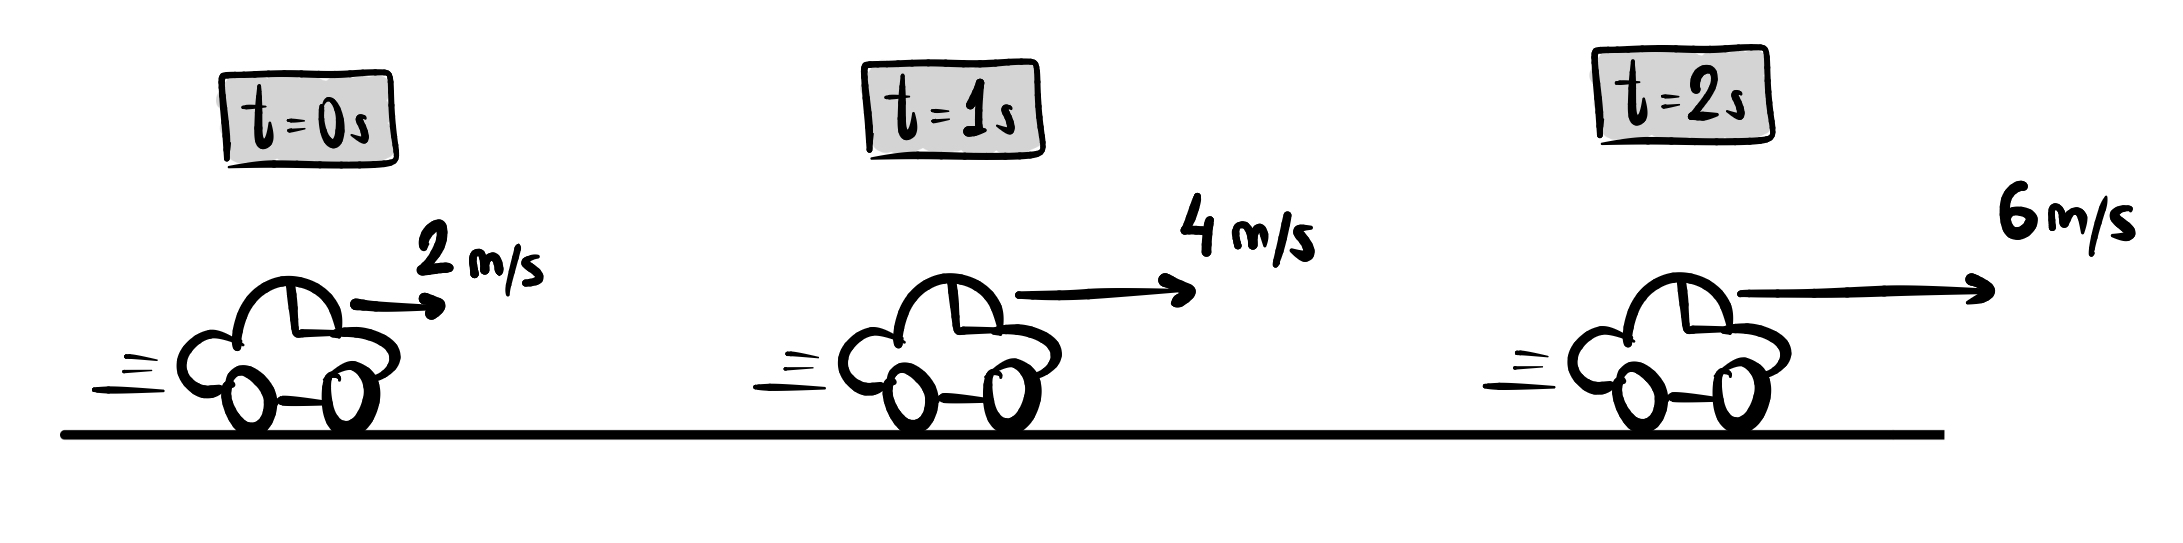
\includegraphics[scale=0.12]{imagensmecanica/muvfuncaovelocidade04.jpeg}
    \caption{Vários instantes para equacionar a função horária da velocidade do MUV.}
    \label{fig_mec_muvfuncaovelocidade04}
\end{figure}

     Contudo, ao escrever a função horária da posição, algum leitor poderia querer ignorar o instante inicial $t=0$s, e escrevê-la a partir do instante $t=1$s, considerando, portanto, o valor de $v_0$ como sendo igual a $4$ m/s, chegando na equação:

     $$ v(t) = 4 +2t.$$

     É imediato perceber que tal equação está errada e não condiz com o contexto, uma vez que, fazendo $t=0$s, chegaríamos em $v(0)=4$m/s, o que claramente está errado, pois $v(0)=2$m/s, como mostra a figura. O erro aqui, portanto, foi não considerar o valor de velocidade inicial como sendo aquele em $t_0=0$s. A equação em que o instante inicial é $t=1$s -- ou qualquer outro -- até pode ser construída, mas não será aquela mesma da Equação \eqref{mecanica_eq_muvfuncaovelocidade}. Neste caso, teríamos que fazer um ajuste e trocar $t$ por $t'=t-1.$ Isso faz a correção para que o novo instante inicial ($t=1$s) seja exatamente $t'=1-1=0$s, ou seja, o instante zero.\footnote{Isso é importante porque o instante de tempo multiplica a aceleração -- o produto $at$ -- e isso representa o incremento de velocidade. Logo, deve-se ter sempre $t=0$ no instante inicial para zerar a variação da velocidade. Uma vez que estamos no instante inicial da análise, não houve, ainda, variação da velocidade.} Neste caso, a equação correta seria:

     $$ v(t') = v_0 + at' \implies v(t)= 4 + 2(t-1).$$
     
     Neste caso, é fácil ver que $v(1) = 4$ m/s, o que concorda com o esperado: em $t=1$s a velocidade é de 4 m/s. 
     
     
     Para o leitor que achou tudo isso complicado demais, fica, portanto, o aviso: para não incorrer neste tipo de complicação e usar sempre a Equação \eqref{mecanica_eq_muvfuncaovelocidade} exatamente naquele formato como construímos, o valor da velocidade inicial $v_0$ deve ser aquele em $t_0=0$s.
     
    \item [(ii)]
     Usar tal equação em contextos nos quais ela não se aplica.

     Faremos aqui uma digressão um pouco mais abstrata, de modo que esse trecho pode ser pulado em uma primeira leitura. Lembre-se que estamos dentro do tópico de Movimento Uniformemente Variado. Correndo o risco de me tornar repetitivo, tal equação é a Função Horária da Velocidade do Movimento Uniformemente Variado -- ou seja, ela serve para computar a velocidade apenas de um corpo que executa um tipo específico de movimento: o movimento com aceleração constante.

     Tentar aplicá-la para outros tipos de movimento levará, naturalmente, a resultados errados. A bem da verdade, se aplicarmos ela para o Movimento Uniforme, até chegamos em um resultado correto. Lembre-se que tal movimento é definido como sendo aquele no qual a velocidade não varia, ou seja, sua aceleração é zero:

     $$ v(t) = v_0 + \cancelto{0}{a} \cdot t \implies \boxed{v(t)=v_0.}$$

     O resultado diz que a velocidade $v(t)$ para qualquer instante de tempo $t$ é igual à velocidade inicial $v_0$, ou seja, tal valor de velocidade é constante e nunca muda -- este é o Movimento Uniforme, e é claro que isso nós já sabíamos. Note, contudo, que, apesar de usarmos a equação ``errada'', nós só chegamos a uma conclusão certa porque, na verdade, o MU é um caso particular do MUV: o Movimento Uniforme é um Movimento Uniformemente Variado em que a aceleração é zero. Logo, todas as equações do MUV, se colocarmos a aceleração igual a zero, devem recair nas equações do MU.\footnote{O leitor pode ver isso como uma grande vantagem: é preciso conhecer só um par de equações -- as funções da posição e da velocidade do MUV, haja vista que as mesmas funções para o MU estão contidas naquelas, bastando, para obtê-las, fazer a aceleração igual a zero. Faça o mesmo exercício, na próxima seção, e obtenha a função da posição do MU a partir daquela do MUV.}

     Tirando este caso particular, em qualquer outro contexto no qual o leitor tentar aplicar a função horária da velocidade do MUV, ele incorrerá em graves erros.
    
    
\end{itemize}


\secgfe{Observações}

Cabe pontuar algumas observações a respeito dos sinais de algumas grandezas na equação. Como já sabemos, o sinal de uma grandeza cinemática -- velocidade ou aceleração -- irá depender do referencial adotado (origem e orientação). Desse modo, é possível escrever a função horária da posição para um certo movimento de mais de uma forma. Observe, para tanto, a Figura \ref{fig_mec_muvfuncaovelocidadesinal01}. Perceba que, nas duas imagens, trata-se exatamente do mesmo movimento -- o que muda é apenas o sistema de orientação: o referencial. Assim, para o referencial da imagem da cima, a velocidade inicial seria positiva, porém a aceleração negativa, de modo que a equação horária da velocidade seria

$$ v(t)=5-2t.$$

A velocidade em um certo instante, digamos $t=5$, seria, portanto, $v(5)=-5$ m/s. Perceba que o sinal negativo, uma vez que o sentido adotado como positivo foi para direita, está indicando apenas que tal velocidade aponta para a esquerda, com intensidade de 5 m/s.



\begin{figure}[h]
    \centering
    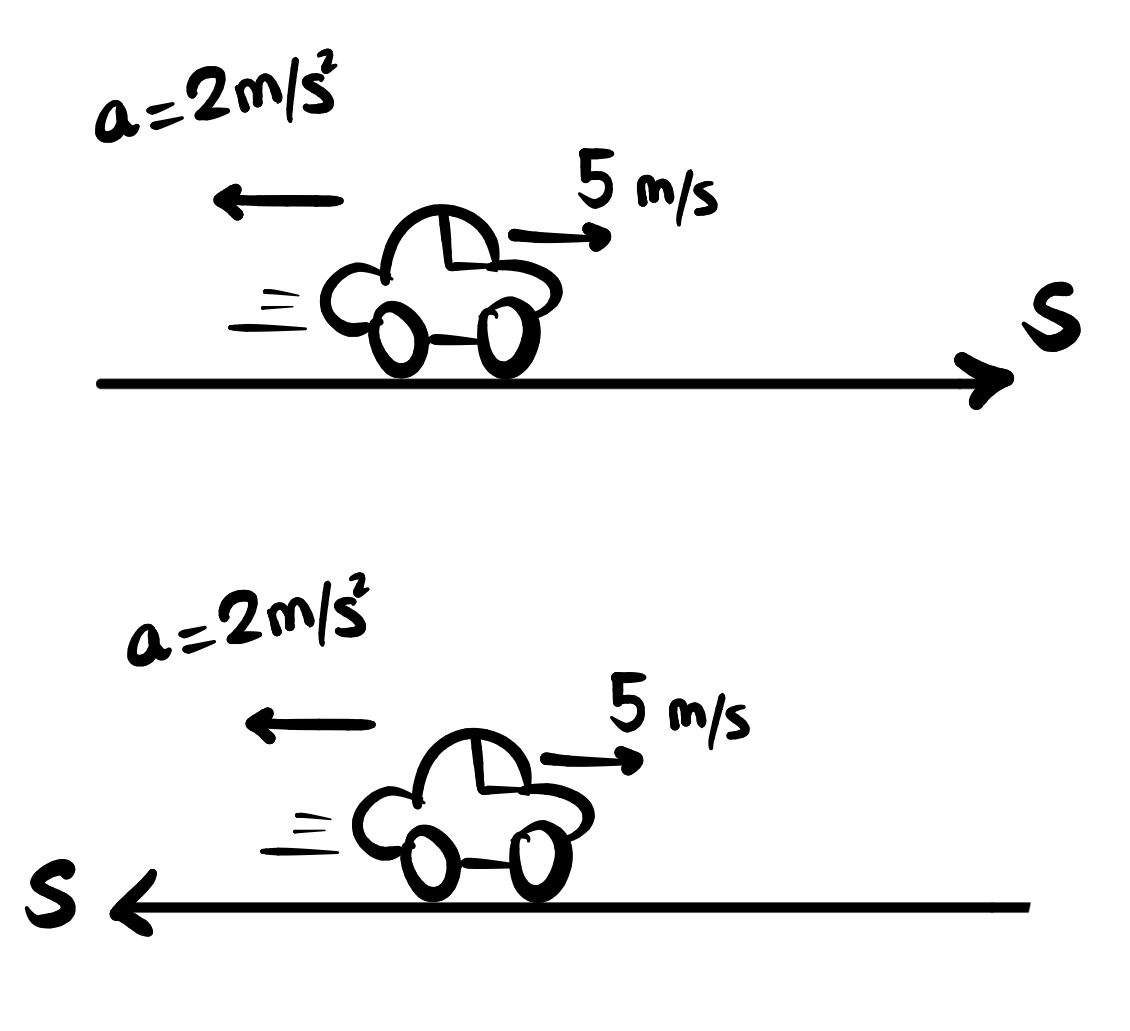
\includegraphics[scale=0.12]{imagensmecanica/muvfuncaovelocidadesinal1.jpeg}
    \caption{Referenciais distintos para equacionar a função da velocidade.}
    \label{fig_mec_muvfuncaovelocidadesinal01}
\end{figure}

Já a mesma equação no referencial da imagem inferior da figura seria diferente: nessa nova escolha de orientação a velocidade inicial é negativa e a aceleração é positiva, de modo que a equação seria:

$$ v(t) = -5+2t,$$
e a velocidade, no mesmo instante $t=5$s, seria $v(5)=5$ m/s. Note que agora a velocidade saiu positiva, o que indica que ela aponta para a esquerda -- uma vez que agora o sentido definido como positivo foi para a esquerda.

Desse modo, usando os dois sistemas de coordenadas distintos, chegamos exatamente à mesma conclusão: a velocidade do carro no quinto segundo de movimento aponta para a esquerda com intensidade de $5$ m/s. É preciso, contudo, saber interpretar os sinais dentro de cada convenção adotada.

Uma observação também merece ser feita a respeito do sinal da aceleração. Um MUV é dito \textbf{acelerado} se a aceleração e velocidade possuem o mesmo sentido, isto é, o mesmo sinal. Isto quer dizer que a velocidade aumenta à medida que o tempo passa. Em contrapartida, o MUV será classificado como \textbf{retardado} caso a velocidade e a aceleração possuam sentidos contrários, ou seja, sinais contrários. Neste caso, o corpo está desacelerando (ou freando), ou seja, ele irá andar cada vez mais devagar até a velocidade zerar.

Dito isso, estudantes costumam se confundir e achar que o movimento será retardado caso a aceleração seja negativa, e acelerado caso ela seja positiva. Note que isso não é verdade, até porque um mesmo movimento pode ter aceleração positiva ou negativa a depender do referencial adotado, como fizemos anteriormente. No primeiro caso a aceleração era positiva e no segundo era negativa -- e o movimento era exatamente o mesmo, só mudamos o sistema de coordenadas usado para descrevê-lo.

Note, portanto, que o que importa para fazer tal tipo de classificação é o sinal da aceleração em relação ao da velocidade: no movimento anterior a velocidade e aceleração sempre possuíam sinais (e portanto sentidos) contrários: inicialmente tínhamos uma velocidade inicial positiva com uma aceleração negativa; ao mudar a orientação passamos a ter uma velocidade inicial negativa e uma aceleração positiva. Nos dois casos os sinais das duas grandezas eram opostos -- indicando que seus sentidos eram opostos -- e, portanto, se velocidade e aceleração possuem sentidos opostos, o movimento é retardado. A Figura \ref{fig_mec_muvfuncaovelocidadestabelasinais} mostra uma tabela com um resumo de todas as possíveis combinações entre os sinais (sentidos) de velocidade e aceleração e o tipo de movimento de cada um deles.

\begin{figure}[h]
    \centering
    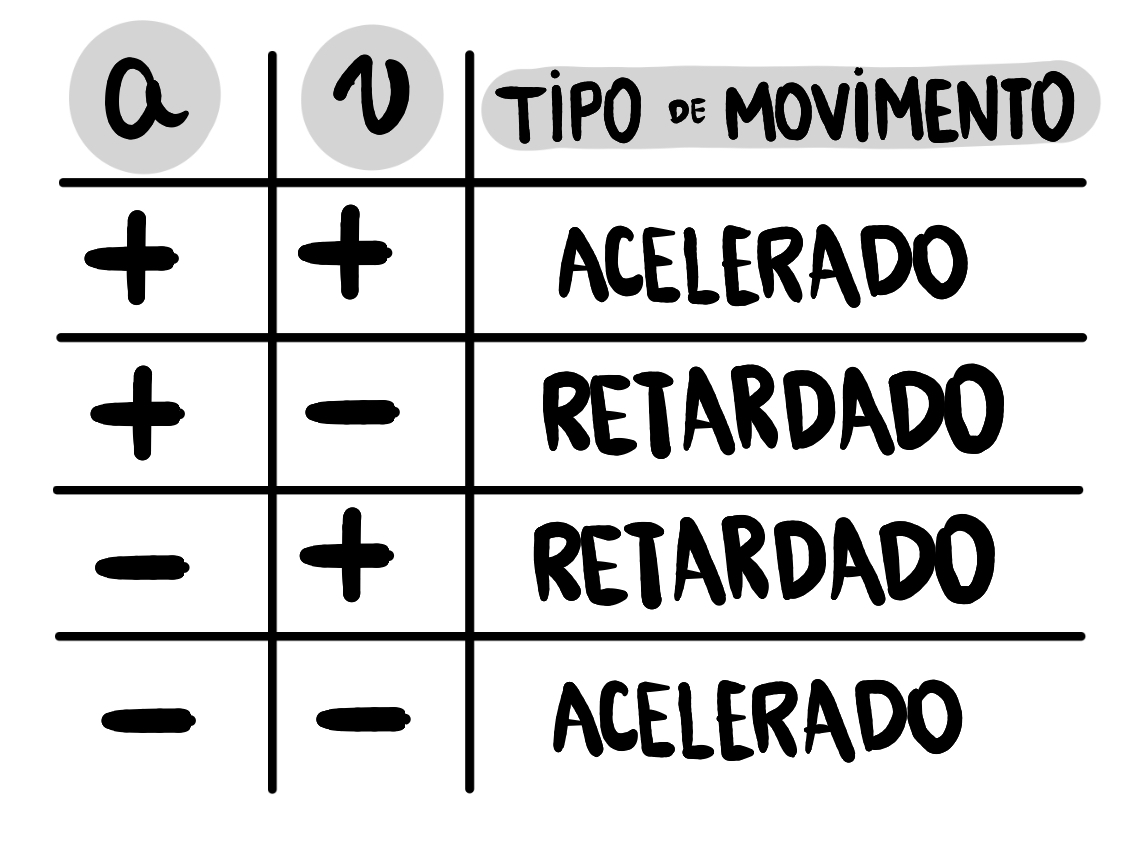
\includegraphics[scale=0.12]{imagensmecanica/muvfuncaovelocidadetabelasinais.jpeg}
    \caption{Classificação do MUV com base na comparação do sentido (sinal) da velocidade e da aceleração.}
    \label{fig_mec_muvfuncaovelocidadestabelasinais}
\end{figure}

%Exemplo resolvido





\vspace{0.3cm}



\begin{exemplo}[Nível I]\label{exemplo_cinematicaescalar_funcaovelocidademuvex01}

Um carro se move com aceleração constante. Sabe-se que, sua velocidade, em um certo instante, é igual a $2$ m/s e, dois segundos após tal instante, a sua velocidade passa a ser de $6$ m/s. Qual é a sua velocidade 10 segundos após ele atingir a velocidade de $6$ m/s?



\resolucao



É interessante fazermos um esboço da situação a fim de não nos perdermos em meio aos dados do problema. Fizemos isso na Figura \ref{fig_mec_funcaovelocidade03}, na qual consideramos o instante inicial do movimento $t_0=0$s como sendo aquele no qual a velocidade vale $2$m/s, que se torna, portanto, a nossa velocidade inicial, ou seja, $v_0 = 2$ m/s.

\vspace{0.3cm}
{
\centering
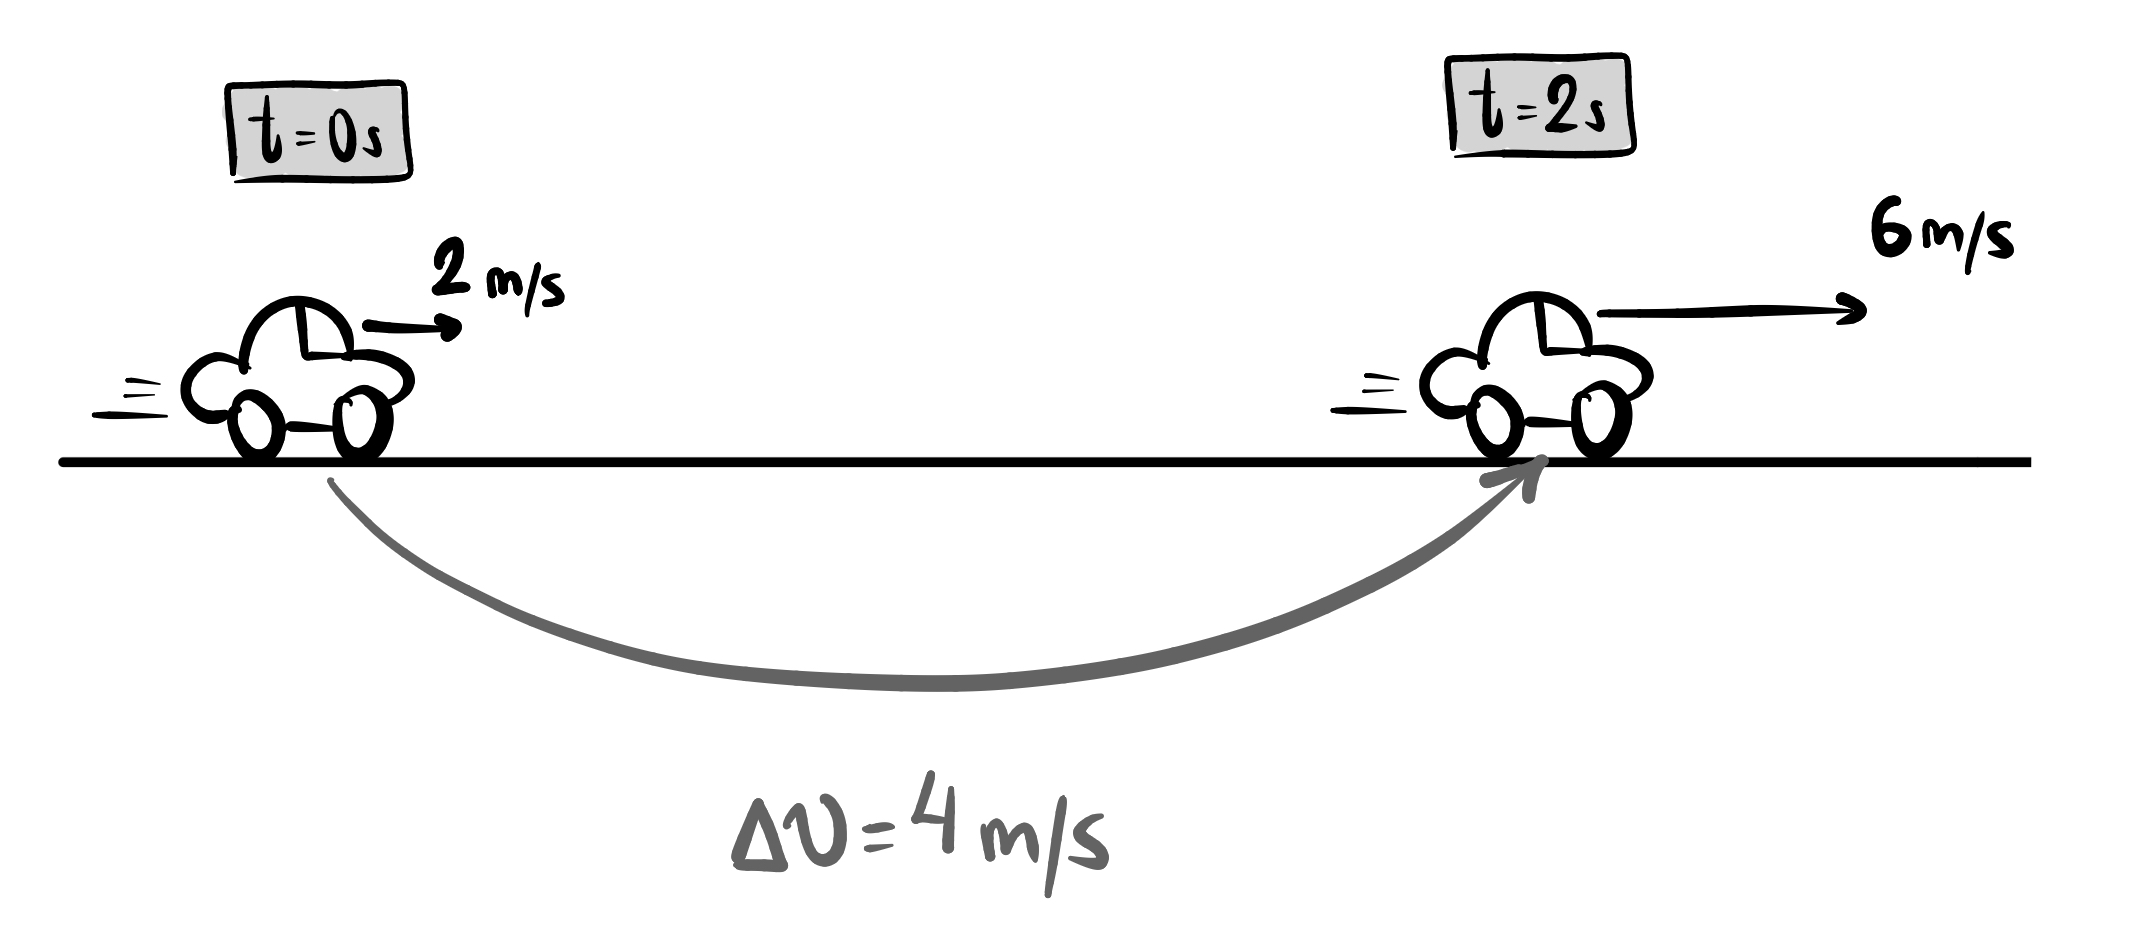
\includegraphics[width=0.5\linewidth]{imagensmecanica/muvfuncaovelocidade03.jpeg}
\captionof{figure}{Referencial orientado para esquerda com origem arbitrária.}
\label{fig_mec_funcaovelocidade03}
} 
\vspace{0.3cm}



Para montar a função horária da velocidade vamos precisar saber qual é a aceleração do carro, o que podemos fazer considerando as informações a respeito dos dois instantes dados:

$$ a = \dfrac{\Delta v}{\Delta t} = \dfrac{6-2}{2-0} = 4 \text{m/s}^2.$$

Munidos de tal valor podemos montar a função horária da velocidade de tal movimento (estamos considerando o sentido positivo para direita):

$$ v = v_0 + at \implies v(t) = 2 + 4t,$$
de modo que agora podemos obter o valor da velocidade $v$ do carro para qualquer instante futuro $t.$ No caso, queremos no instante de tempo 10s após o carro atingir a velocidade de 6 m/s, que é o instante $t=2$s em nossa análise.\footnote{Lembre-se de que o instante inicial $t_0=0$s é aquele no qual a velocidade é $v_0$, o qual consideramos sendo a velocidade de 2 m/s, e não 6 m/s. } Assim, 10s após isso, estaremos no instante $t=12$s, de modo que a velocidade em tal momento é dada por 
$$v(12)=2+4\cdot12 = \boxed{50 \text{m/s}.}$$

\end{exemplo}






\vspace{0.3cm}





\begin{exemplo}[Nível II]\label{exemplo_cinematicaescalar_funcaovelocidademuvex02}




Considere uma bola, lançada verticalmente para cima, em $t=0$, com velocidade de $30$ m/s. Se a aceleração da gravidade é igual a $10$ m/s$^2$, calcule:

\begin{enumerate}
    \item [(a)] O instante de tempo no qual a bola inverte o sentido do movimento.
    \item [(b)] A velocidade da bola em $t=5$s.
\end{enumerate}


\resolucao


\begin{enumerate}
    \item [(a)] O instante de tempo no qual um corpo em MUV inverte o sentido do movimento sempre será aquele no qual a velocidade é $0.$ Isso porque, se o corpo está sendo desacelerado, ele o será até que sua velocidade seja totalmente diminuída, ou seja, ela chegue em zero. Daí em diante, caso a mesma aceleração que o freou permaneça atuando, ela começará a acelerar o corpo no sentido contrário ao qual ele se movia -- a mesma aceleração gera, agora, um movimento acelerado, e não mais retardado.

    Logo, a bola chegará no ponto de altura máxima -- posição em que sua velocidade zera -- e inverterá seu sentido do movimento quando

    $$ v(t) = v_0+at =0\implies v(t) = 30-10t =0 \implies \boxed{t=3 \text{ s,}}  $$

    \noindent em que consideramos um sistema de coordenadas orientado para cima.


    
    \item [(b)] Alguns leitores poderiam pensar que é preciso construir uma nova função horária da velocidade após $t=3$s, haja vista que agora o movimento se dá em um sentido contrário, e deixou de ser retardado para ser acelerado.

    Isso é um equívoco, e tal construção é totalmente desnecessária. O fato de que o movimento mudou de sentido já é capturado pela função horária da velocidade por meio do sinal: no sistema que adotamos, orientado para cima, velocidades para cima são positivas e velocidades para baixo são negativas. 

    Logo, note que, quando o corpo começa a cair, sua velocidade ficará negativa -- a própria equação já conterá essa informação -- e, sendo a aceleração da gravidade negativa (uma vez que ela está orientada para baixo) teremos a velocidade e a aceleração com mesmo sinal, isto é, mesmo sentido, o que já captura informação de que o movimento passou a ser acelerado. 

    Portanto, para qualquer instante de tempo podemos usar a mesma equação $v(t)=30-10t,$ de modo que, em $t=5$s, teremos:

    $$ v(5)=30-10\cdot 5 \implies v(5)=-20 \text{ m/s},$$

    \noindent o que quer dizer uma velocidade com valor de $20$ m/s orientada para baixo. Veja que isso é condizente com o esperado: após $t=3$s quaisquer velocidades informadas pela equação devem ser negativas, uma vez que o sentido do movimento se inverte naquele instante.

    
\end{enumerate}

\end{exemplo}




\vspace{0.3cm}



% \begin{exemplo}[Nível III]\label{exemplo_cinematicaescalar_funcaovelocidademuvex03}



% \resolucao


% \end{exemplo}






% \vspace{0.3cm}






\begin{secnivel}[Função Horária da Posição do MUV]{I}{Função Horária da Posição do Movimento Uniformemente Variado}
 

  \eqLdois{dem}{mecanica_eq_muvfuncaoposicao}{\Delta s = v_0t + \dfrac{1}{2}at^2 \quad \text{ou} \quad  s = s_0+v_0t + \dfrac{1}{2}at^2 }
  
\end{secnivel}








\secgfe{De onde vem}

Antes de dar sequência a essa demonstração, é importante que o leitor tenha passado com calma e compreendido por completo o conteúdo do Apêndice \ref{apendice_areagraficovxt}. Feito isso, para demonstrar tal equação usaremos justamente o fato de que a área abaixo do gráfico de velocidade por tempo fornece o deslocamento $\Delta s$ do corpo naquele intervalo de tempo. 

Para o MUV, sabemos que a velocidade varia no tempo de acordo com a Equação \eqref{mecanica_eq_muvfuncaovelocidade}, que é uma função afim, cujo gráfico é uma reta. Tal reta se encontra representada na Figura \ref{fig_mec_graficovxt}, na qual usamos, novamente, a Equação \eqref{mecanica_eq_muvfuncaovelocidade} para marcar que a velocidade da partícula no instante $t$ será $(v_0+at).$

\begin{figure}[h]
    \centering
    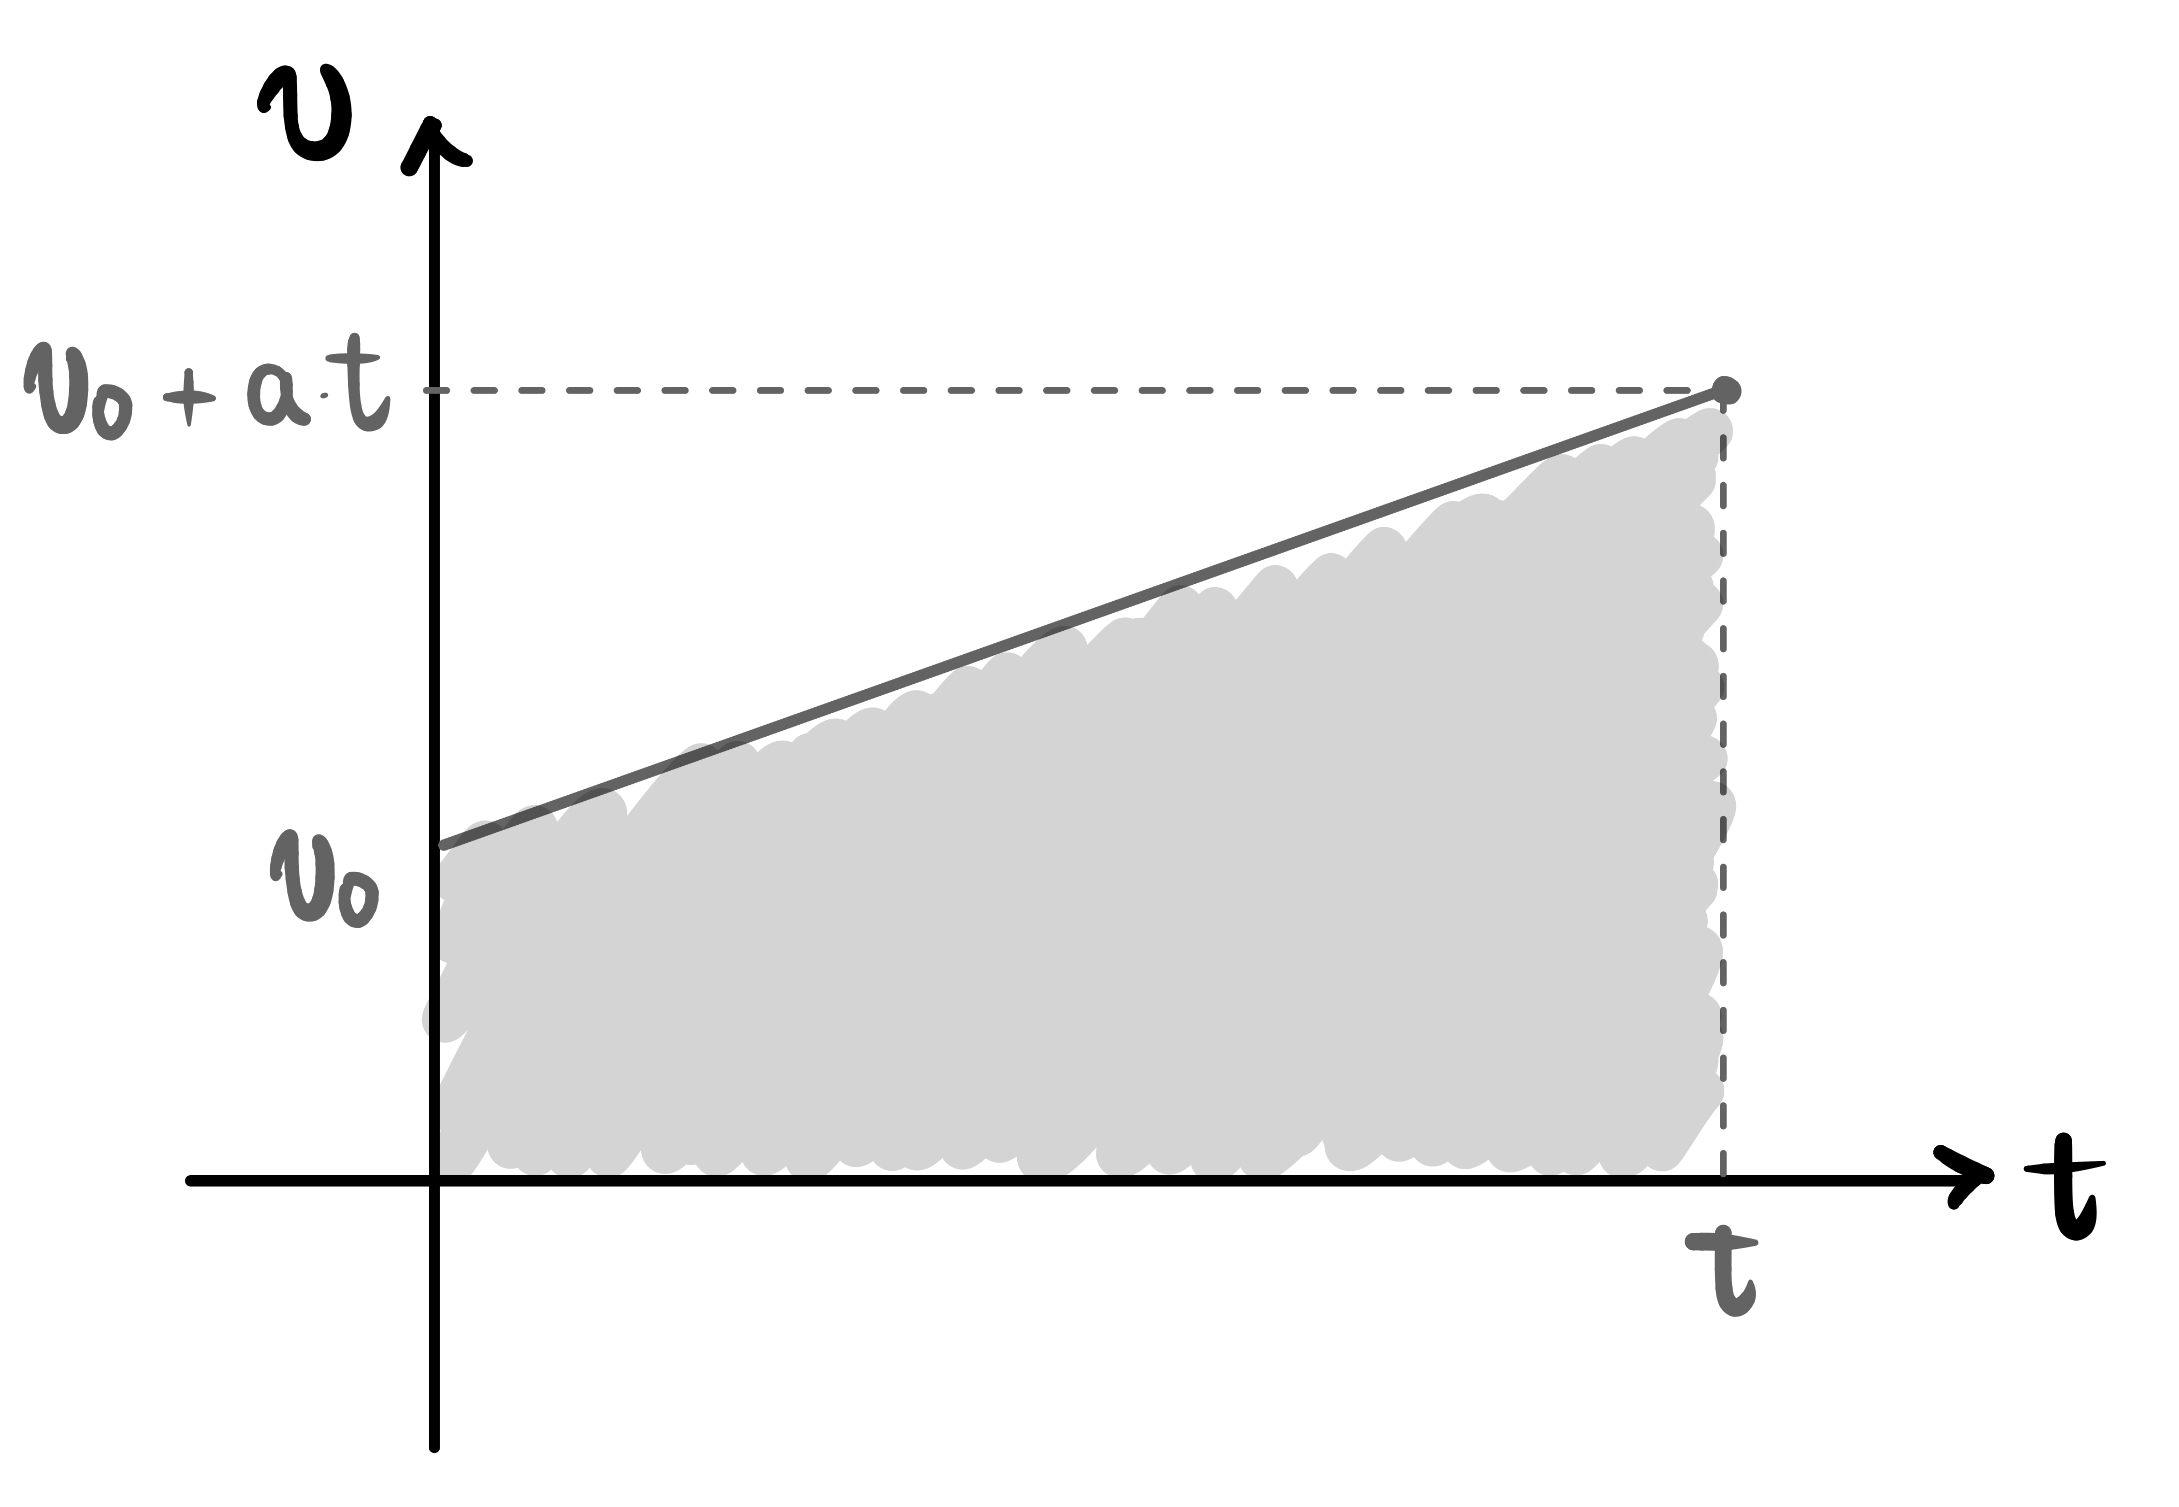
\includegraphics[scale=0.09]{imagensmecanica/muvgraficovxt.jpeg}
    \caption{Gráfico $v$ por $t$ para o MUV. }
    \label{fig_mec_graficovxt}
\end{figure}

O deslocamento da partícula no intervalo de $0$ a $t$ será, portanto, a área abaixo do gráfico ao longo deste intervalo, que incorre em ser a área de um trapézio, de altura $t$ e bases $v_0$ e $(v_0+at),$ sendo sua área $A$ dada por

$$ A=\Delta s = \dfrac{(B+b)\cdot h}{2}= \dfrac{(v_0+(v_0+at))\cdot t}{2} = \dfrac{2v_0t+at^2}{2} \implies \boxed{\Delta s = v_0t + \dfrac{1}{2}at^2.} $$

Sendo o deslocamento $\Delta s$ igual à variação da posição, isto é, sendo $s$ a posição da partícula no instante $t$ e $s_0$ sua posição no instante inicial $t=0$s, temos que $\Delta s = (s-s_0),$ de modo que a equação acima pode ser escrita como

$$ s=s_0+ v_0t + \dfrac{1}{2}at^2.$$

A Equação \eqref{mecanica_eq_muvfuncaoposicao} é o análogo da Equação \eqref{mecanica_eq_mu_funcaoposicao}, porém essa descreve a evolução da posição no Movimento Uniforme, enquanto aquela descreve como a posição evolui no Movimento Uniformemente Variado.\footnote{Note, inclusive, que ao tornar a aceleração nula na Equação \eqref{mecanica_eq_muvfuncaoposicao}, desaguamos justamente na função horária da posição do MU -- na qual $v_0=v$, haja vista que a velocidade é constate e nunca muda. Isso tem a ver com  fato anteriormente discutido de que o MU é um caso particular do MUV para o qual a aceleração tem o específico valor zero.}

\secgfe{Onde é usada}

Em qualquer contexto que se deseje computar a distância percorrida ou estudar a evolução das posições de um objeto que se move com aceleração constante. Considere, por exemplo, um carro que se move com aceleração de 6 m/s$^2$, que aponta no mesmo sentido da sua velocidade, que, inicialmente, é de 10 m/s. Se a posição inicial deste carro é no quilômetro 40 de uma rodovia, qual será a sua posição após 15 minutos de viagem?

Montando a função horária da posição para tal movimento, teremos (atente-se às unidades de medida):

$$ s(t)=s_0+v_0t +\dfrac{1}{2}at^2 \implies s(t)=40.000+10t+3t^2.$$

Note que tal equação nos possibilita descobrir aonde o carro estará, isto é, qual é a sua posição $s(t)$, para qualquer instante de $t$ futuro. Em particular, após 15 minutos, que são $15*60=900$ segundos, a posição do carro será

$$s(900)= 40.000+10\cdot 900+3 \cdot 900^2 \implies \boxed{ s(900)=2.479.000 \text{m}=2.479 \text{km},}$$
ou seja, o carro estará para lá do quilômetro dois mil da rodovia.\footnote{Caso o leitor tenha achado tal número estranho, reitero que ele é factível -- pelo menos em termos da geografia do Brasil. A BR-116, que conecta Fortaleza ao Rio Grande do Sul, possui cerca de 4.600 km de extensão. Contudo, certamente é impossível percorrê-la em 15 ou 30 minutos, de carro. O que acontece é que uma aceleração de 6 m/s$^2$, apesar de ser possível para um carro, não pode jamais ser mantida por 15 minutos. Com tal valor de aceleração, um carro vai de 0 a 100 km/h em cerca de 5 segundos. Logo, se ele conseguisse manter essa aceleração pelos próximos 14 minutos e 55 segundos seguintes, ele alcançaria uma velocidade de quase 20 mil km/h, o que certamente o leitor nunca deve ter visto acontecendo por aí. }



\secgfe{Erros comuns}

O erro mais comum aqui é o estudante usar a função horária da posição do MU quando o movimento é acelerado. Ou seja, é como se ele acabasse esquecendo para trás o fator $\sfrac{at^2}{2}.$

É importante notar que as Equações \eqref{mecanica_eq_mu_funcaoposicao} e \eqref{mecanica_eq_muvfuncaoposicao} de fato guardam similaridades: as duas se propõem a fazer a mesma coisa -- dizer como a posição de um corpo evolui no tempo ao longo de seu movimento. Contudo, elas o fazem para movimentos distintos: uma delas é para o movimento com velocidade constante, a outra para o movimento com aceleração constante. Movimentos de natureza e características distintas, naturalmente, terão equações diferentes para descrever sua evolução.

\secgfe{Observações}


É importante notar que a Equação \eqref{mecanica_eq_muvfuncaoposicao}, em seu primeiro formato, calcula o deslocamento do corpo, e não a distância percorrida. Para deixar isso claro, considere um corpo em um MUV em que sua velocidade inicial é de $30$ m/s e sua aceleração é de $10$ m/s$^2$, contrária ao sentido da velocidade inicial. Pede-se calcular a distância percorrida por tal corpo ao longo dos primeiros 6 segundos de movimento.

O estudante mais desavisado poderia escrever que

$$ d=v_0t+\dfrac{1}{2}at^2 \implies d = 30t+\dfrac{1}{2}(-10)t^2 \implies d=30 \cdot 6 -5 \cdot 6^2 \implies \boxed{d=0\text{m}.}$$

Como pode um corpo estar se movendo -- de forma acelerada, inclusive --  percorrer uma distância nula? Naturalmente, tal resultado está errado. E o erro foi em considerar que deslocamento $\Delta s$ é igual à distância percorrida. Novamente, note que a Equação \eqref{mecanica_eq_muvfuncaoposicao} fornece o \textbf{deslocamento} do corpo em MUV, e \textbf{não a distância que ele percorre}. Ou seja, o que calculamos acima, na verdade, é que $\Delta s=0$m, o que não é incoerente com o tipo de movimento. O que isso quer dizer é que o corpo, no sexto segundo de movimento, retorna para a mesma posição em que ele estava quando o movimento iniciou.

Isso não é incoerente porque o movimento, inicialmente, é retardado: a aceleração é contrária à velocidade. Isso quer dizer que o nosso objeto terá sua velocidade diminuída até zerar. Caso a aceleração continue existindo, ela irá, a partir do momento em que a velocidade zera, começar a fazer o objeto ganhar movimento no sentido oposto, ou seja, o objeto começa a ``voltar'', de modo que, em algum momento, ele passará de volta pela sua posição inicial. Neste instante, seu deslocamento total é nulo -- a posição inicial e final são iguais.

Tal situação -- que é justamente a do problema -- está descrita na Figura \ref{fig_mec_muvlancamentovertical}. Note que, ao longo dos primeiros 3 segundos de movimento, a velocidade vai de $30$ m/s a $0$ m/s. Daí em diante, o movimento é simétrico: o corpo inverte o sentido do seu movimento e a velocidade agora vai de $0$ m/s a $30$ m/s -- o sinal negativo só indica que, agora, o sentido do movimento inverteu. Assim, nos primeiros 6 segundos de movimento, o objeto sobe, atinge a altura máxima e retorna à mesma posição inicial, de modo que o deslocamento total é nulo. Essa é a exata experiência que o leitor pode ter ao lançar verticalmente para cima uma pedra.

\begin{figure}[h]
    \centering
    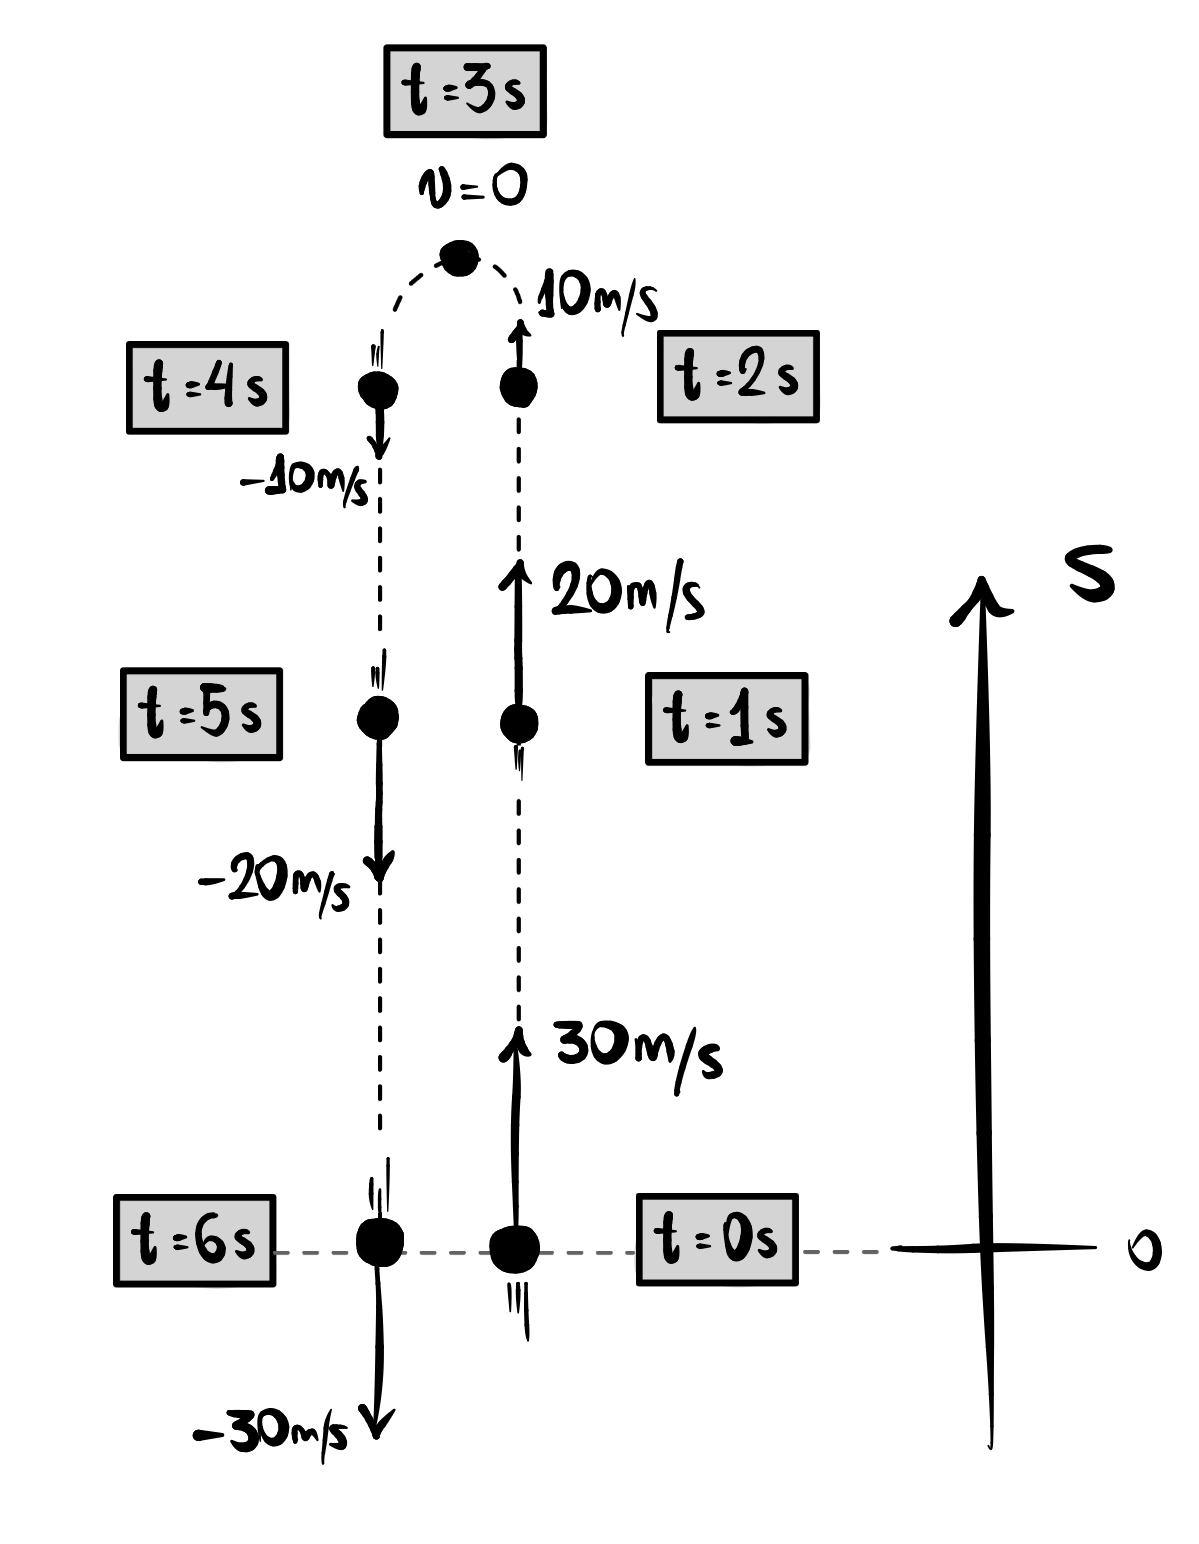
\includegraphics[scale=0.18]{imagensmecanica/muvfuncaoposicaoexemplo.jpeg}
    \caption{O lançamento vertical de uma pedra e o deslocamento total nulo.}
    \label{fig_mec_muvlancamentovertical}
\end{figure}

Como poderíamos perceber e computar tudo isso, sem o auxílio da Figura \ref{fig_mec_muvlancamentovertical}? Perceba que, em qualquer movimento retardado, este é um cuidado que o leitor deverá tomar. Porque em um movimento acelerado o sentido do movimento nunca muda, de modo que a distância sempre coincidirá com o deslocamento, e o raciocínio feito anteriormente estaria sempre correto.

Contudo, em um movimento retardado, eventualmente o sentido do movimento pode mudar, de modo que distância e deslocamento deixarão de coincidir, e é aí onde deve-se tomar cuidado. Para saber se isso ocorreu, é preciso descobrir quando a velocidade zera, porque é a partir daí que o sentido do movimento irá inverter. Para o movimento do exemplo, começamos com $v_0= 30$ m/s e $a=-10 $ m/s$^2$ (estamos considerando o sentido positivo como sendo aquele para onde aponta a velocidade inicial). Neste caso, a função horária da velocidade -- Equação \eqref{mecanica_eq_muvfuncaovelocidade} -- de tal movimento é

$$ v(t)=v_0+at \implies v(t) = 30 - 10t.$$

Queremos saber em qual instante a velocidade zera, isto é:

$$v(t)=30-10t =0 \implies \boxed{t=3\text{s.}}$$


Ora, acabamos de descobrir que a velocidade zera no terceiro segundo de movimento. Isso quer dizer que, nos primeiros 3 segundos de movimento, distância e deslocamento coincidem: o movimento se dá ao longo de um mesmo sentido (a Figura \ref{fig_mec_muvlancamentovertical} evidencia isso). Daí em diante o sentido do movimento irá inverter, e a distância e o deslocamento deixarão de coincidir. Sendo assim, a fim de computar a distância total percorrida por tal objeto nos primeiros 6 segundos de movimento, teríamos que calcular primeiro o seu deslocamento ao longo dos três primeiros segundos -- porque ele coincide com a distância -- e depois seu deslocamento do segundo 3 ao segundo 6, que também coincidirá com a distância neste intervalo.

Para os primeiros 3 segundos teríamos:

$$d_1=\Delta s_1=v_0t+\dfrac{1}{2}at^2 \implies d_1 = 30t +\dfrac{1}{2}(-10)t^2 \implies d_1 =30\cdot 3 -5 \cdot 3^2 \implies \boxed{d_1=45\text{m}.}$$


A partir de agora, teríamos que computar o deslocamento nos 3 segundos subsequentes. Contudo, percebendo que o movimento é simétrico -- a distância percorrida na subida, nos primeiros 3 segundos, é igual à distância percorrida na descida, nos próximos 3 segundos -- poderíamos de imediato concluir que a distância total percorrida é o dobro do valor anteriormente calculado, isto é $D=2d_1= \boxed{90 \text{m}.}$

\begin{figure}[h]
    \centering
    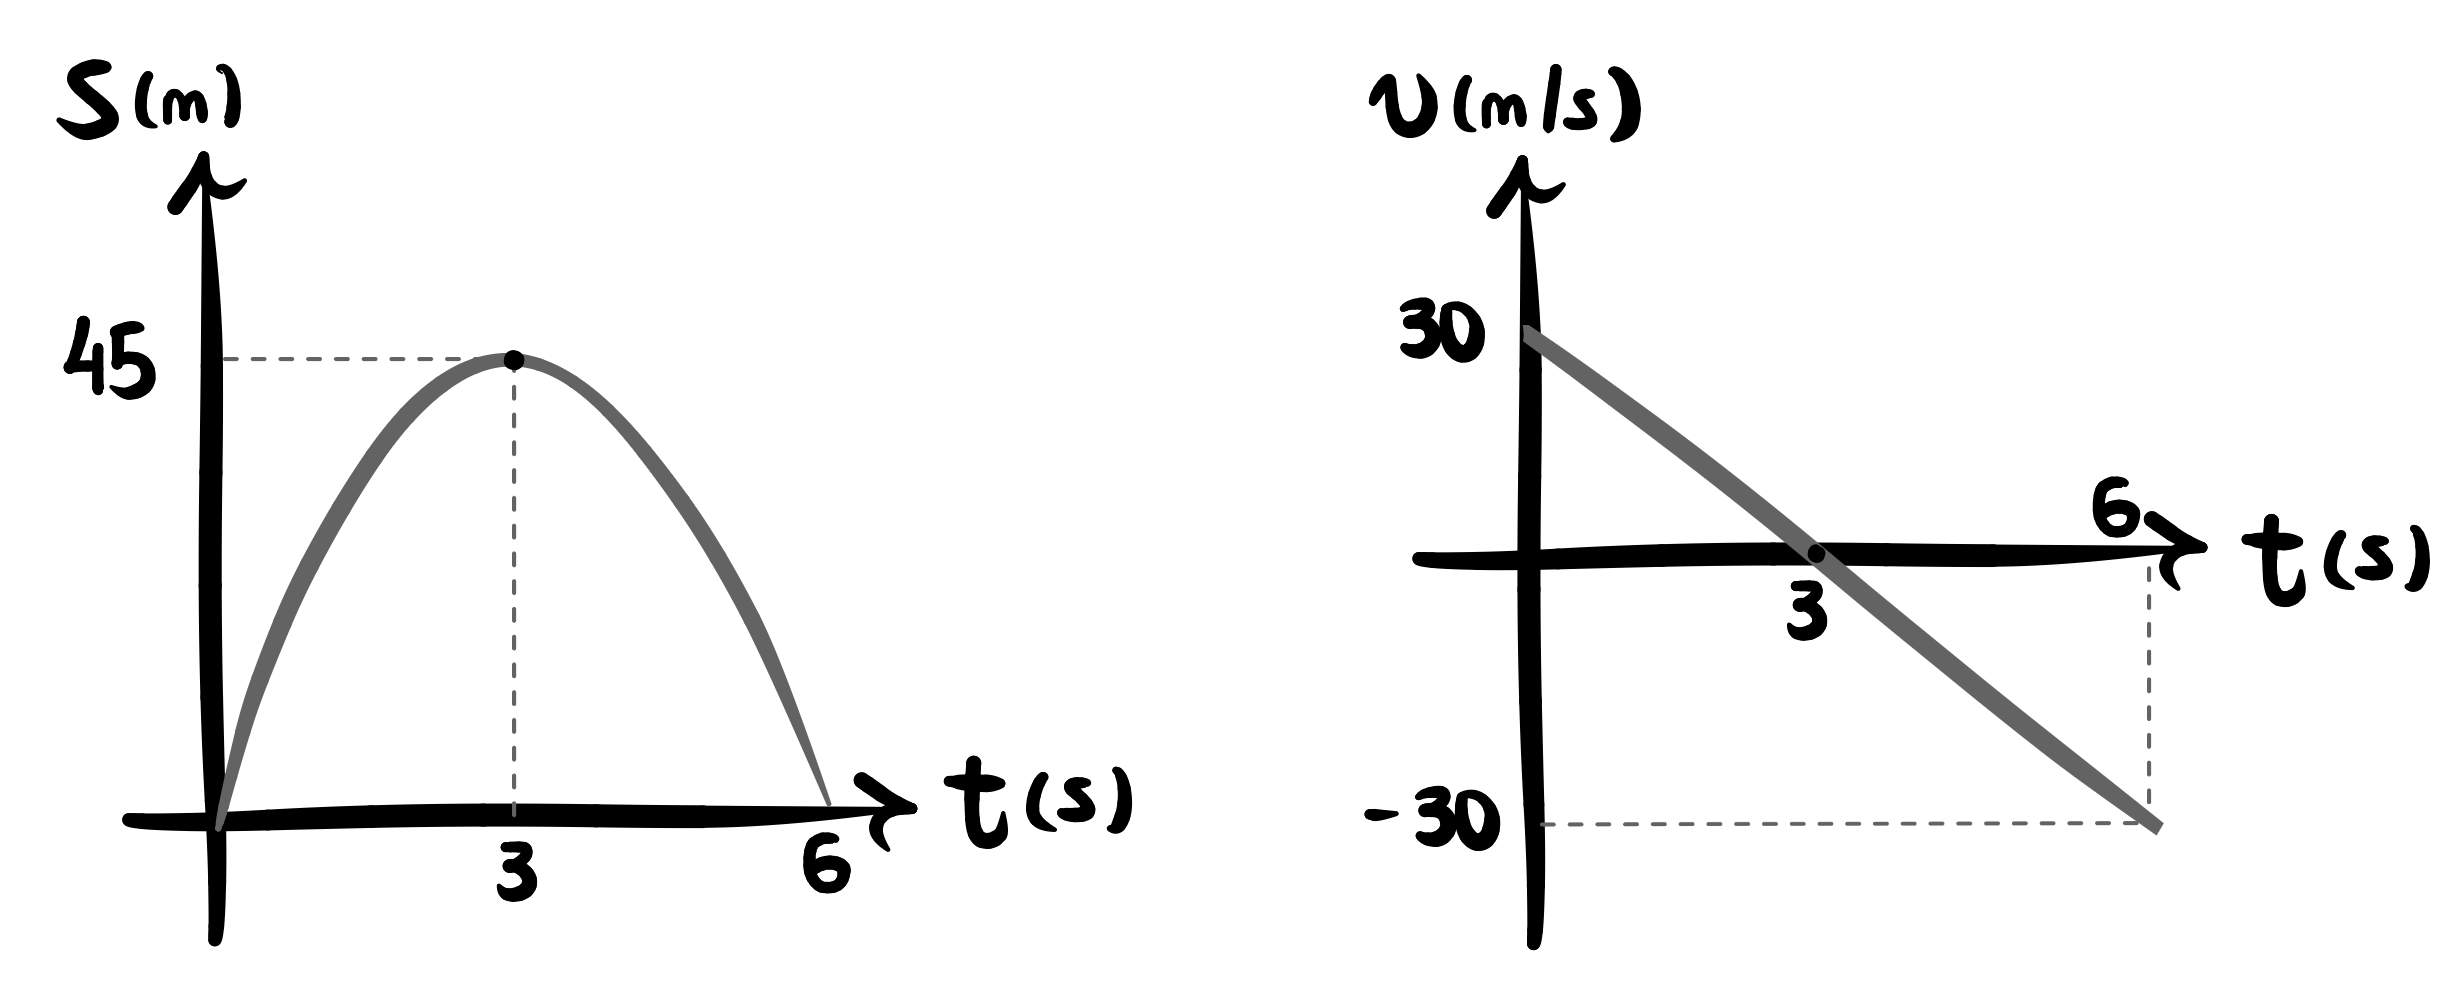
\includegraphics[scale=0.28]{imagensmecanica/graficosmuv.png}
    \caption{Os gráficos de posição e velocidade por tempo do movimento da pedra da Figura \ref{fig_mec_muvlancamentovertical}.}
    \label{fig_mec_graficosmuv}
\end{figure}

A Figura \ref{fig_mec_graficosmuv} mostra os gráficos de posição e velocidade por tempo, respectivamente, do movimento da pedra. Note, no gráfico de posição por tempo, que a posição aumenta até o terceiro segundo -- ponto em que a posição (altura) da pedra é máxima -- e passa a regredir deste instante em diante. Ou seja, o sentido do seu movimento deve inverter a partir de $t=3$s. O gráfico da direita, da velocidade por tempo, é compatível com isso: a velocidade é positiva nos primeiros 3 segundos, zerando em $t=3$s e se tornando negativa daí em diante. A inversão do sinal da velocidade indica a inversão no sentido do movimento.

%Exemplo resolvido

\vspace{0.3cm}

\begin{exemplo}[Nível I]\label{exemplo_cinematicaescalar_funcaoposicaomuvex01}


Uma câmera eletrônica está instalada em $s=0$ em uma certa avenida. Um carro passa por este ponto no instante $t=0,$ com velocidade de 15 m/s. A partir desse instante, o carro passa a acelerar uniformemente com aceleração de $2$m/s$^2$.

\begin{itemize}
    \item [(a)] Qual é a posição do carro após 10s?
    \item [(b)] Em qual instante o carro atinge a posição $s=1$km?
\end{itemize}



\resolucao



Convencionemos que o sentido positivo é aquele para o qual aponta a velocidade do carro. Neste caso, a função horária da posição do seu movimento é dada por

$$ s= s_0+v_0t+\dfrac{1}{2}at^2 \implies \boxed{ s(t)=15t+t^2.}$$

\begin{itemize}
    \item [(a)] Em $t=10$s a posição do carro será dada por:
    $$ s(10)=15 \cdot 10 + 10^2 = \boxed{250 \text{m}.}$$

    \item [(b)] Para saber em qual instante de tempo o carro alcança a posição $s=1000$m precisamos resolver a equação:

    $$ s(t)= 15t+t^2 = 1000 \implies t^2+15t-1000=0,$$
    cujas soluções são $t_1=-40$s e $t_2=25$s. Descartamos, naturalmente, a primeira solução, por ser negativa e não ter sentido físico. Assim, o carro atinge a posição $s=1$km em \boxed{$t=25$ \text{s}.}
\end{itemize}

\end{exemplo}


\vspace{0.3cm}





\begin{exemplo}[Nível II (ITA 2016)]\label{exemplo_cinematicaescalar_funcaoposicaomuvex02}


A partir do repouso, um foguete de brinquedo é lançado verticalmente do chão,
mantendo uma aceleração constante de $5{,}00\ \text{m/s}^2$ durante os
$10{,}0$ primeiros segundos. Desprezando a resistência do ar, a altura máxima
atingida pelo foguete e o tempo total de sua permanência no ar são,
respectivamente, de

\begin{enumerate}
  \item [(a)] $375\ \text{m}$ e $23{,}7\ \text{s}$
  \item [(b)] $375\ \text{m}$ e $30{,}0\ \text{s}$
  \item [(c)] $375\ \text{m}$ e $34{,}1\ \text{s}$
  \item [(d)] $500\ \text{m}$ e $23{,}7\ \text{s}$
  \item [(e)] $500\ \text{m}$ e $34{,}1\ \text{s}$
\end{enumerate}

\resolucao



Vamos dividir o estudo do movimento em duas partes:

\begin{enumerate}
    \item [(i)] Primeiros 10 segundos de movimento.

  Considere um sistema de coordenadas com origem na posição inicial do foguete, no chão, e com orientação para cima. Assim, a função horária da posição do foguete é
  $$ s= \cancelto{0}{s_0}+\cancelto{0}{v_0}+\dfrac{1}{2}5t^2 \implies \boxed{s(t)=\dfrac{5}{2}t^2.}$$

  Após 10 segundos sua posição será, naturalmente, $s(10)= \sfrac{5}{2}\cdot 10^2 = 250$m. Já a função horária da velocidade do foguete é

  $$ v= \cancelto{0}{v_0}+at \implies \boxed{v(t)=5t,}$$

  \noindent de modo que sua velocidade, em $t=10$s, é $v(10)=5\cdot 10=50$ m/s.

  \item[(ii)] Consideramos o movimento a partir de $t=10$s, no qual o foguete desligou sua aceleração. A partir de agora, é como se tivéssemos um lançamento vertical para cima, com velocidade inicial de $50$ m/s e sendo desacelerado pela gravidade, com aceleração de $g=10$m/s$^2.$ A função horária da velocidade é

  $$ v(t')=v_0+at' \implies \boxed{v(t')=50-10t',}$$

 \noindent e sua função horária da posição é

 $$s(t') = s_0 + v_0t'+ \dfrac{1}{2}at'^2 \implies \boxed{s(t')=250+50t'-5t'^2.}$$

 Perceba que estamos usando o mesmo referencial: orientado para cima e com origem no chão -- é por isso que agora a posição inicial do objeto é $s_0=250$m. O que mudamos foi apenas o tempo: é como se tivéssemos, a partir do ponto no qual o foguete está na posição $s=250$m, soltado um novo cronômetro, que marca o tempo $t'.$ É importante destacar essa diferença porque este tempo $t'$ está 10 segundos atrás do nosso tempo $t$ inicial, ou seja, $t'=t-10.$ Logo, quando $t=10$s, teremos $t'=0,$ que é a situação a partir da qual começaremos a equacionar. Dito isso, queremos que o foguete retorne ao chão, ou seja, sua posição final deve voltar a ser $s=0:$

 $$ s(t')=250+50t'-5t'^2=0 \implies \boxed{t'=5\pm5\sqrt3.}$$

 Uma das soluções da equação quadrática é negativa, de modo que a desprezamos. Assim, o instante de tempo até que o foguete retorne ao solo é $t'=5+5\sqrt3 \approx 13,65$ segundos. Logo, como $t'=t-10,$ segue que o tempo total, a partir do lançamento do foguete, até que ele retorne ao solo, é

 $$ t = t'+ 10 = 13,65 + 10 \implies \boxed{t=23,65 \text{ segundos.}} $$

 A altura máxima ocorrerá quando a velocidade tiver zerado, ou seja:

 $$ v(t')=50-10t' = 0 \implies \boxed{t'=5 \text{ segundos,}}$$

\noindent instante no qual a posição do foguete será

$$ s(t')=250+50t'-5t'^2 \implies s(5)=250+50 \cdot 5 -5 \cdot 5^2 \implies \boxed{ s(5)= 375 \text{ metros,}} $$

 \noindent de modo que a letra A fica sendo a resposta.
    
\end{enumerate}

  

\end{exemplo}

\vspace{0.3cm}





\begin{exemplo}[Nível III (ITA 2003)]\label{exemplo_cinematicaescalar_funcaoposicaomuvex03}

A partir do repouso, uma pedra é deixada cair da borda no alto de um edifício. 

{
\centering
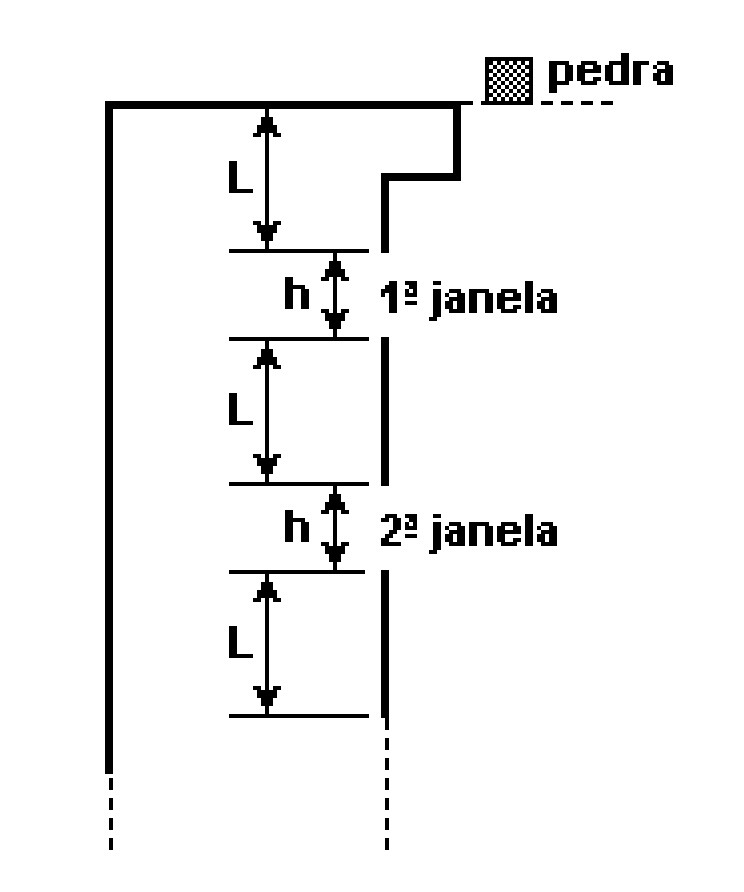
\includegraphics[width=0.25\linewidth]{imagensmecanica/funcaoposicaomuvITAexemplo.png}
\captionof{figure}{}
\label{fig_mec_funcaoposicaomuvITAjanelaexemplo}
} 

A figura mostra a disposição das janelas, com as pertinentes alturas $h$ e distâncias $L$ que se repetem igualmente para as demais janelas, até o térreo. Se a pedra percorre a altura $h$ da primeira janela em $t$ segundos, quanto tempo levará para percorrer, em segundos, a mesma altura $h$ da quarta janela? (Despreze a resistência do ar.)

\begin{enumerate}
  \item [(a)] 
  \left(
  \frac{\sqrt{L+h}-\sqrt{L}}
       {\sqrt{2L+2h}-\sqrt{2L+h}}
  \right)t$
  
  \item [(b)]
  \left(
  \frac{\sqrt{2L+2h}-\sqrt{2L+h}}
       {\sqrt{L+h}-\sqrt{L}}
  \right)t$
  
  \item [(c)]
  \left(
  \frac{\sqrt{4(L+h)}-\sqrt{3(L+h)+L}}
       {\sqrt{L+h}-\sqrt{L}}
  \right)t$
  
  \item [(d)]
  \left(
  \frac{\sqrt{4(L+h)}-\sqrt{3(L+h)+L}}
       {\sqrt{2L+2h}-\sqrt{2L+h}}
  \right)t$
  
  \item [(e)]
  \left(
  \frac{\sqrt{3(L+h)}-\sqrt{2(L+h)+L}}
       {\sqrt{L+h}-\sqrt{L}}
  \right)t$
\end{enumerate}


\resolucao



Considere um eixo vertical orientado para baixo com origem na posição em que a pedra é abandonada. Logo, a função horária da posição da pedra é

$$ s(t)=\cancelto{0}{s_0}+\cancelto{0}{v_0}t+\dfrac{1}{2}at^2 \implies s(t)=\dfrac{g}{2}t^2.$$

Sejam $s_{A}$ e $s_{B}$ as posições da pedra logo antes de adentrar na região da primeira janela e logo depois de tê-la percorrido. Sejam $t_A$ e $t_B$ os instantes de tempo respectivos de tais posições, de modo que, pelo enunciado, temos que $t_B - t_A = t.$ Assim, temos:

\begin{align}
    s_A &= L = \dfrac{g}{2}t_A^2 \implies t_A = \sqrt{\dfrac{2L}{g}}. \nonumber \\
    s_B &= L+h = \dfrac{g}{2}t_B^2 \implies t_B = \sqrt{\dfrac{2(L+h)}{g}}. \nonumber 
\end{align}

Subtraindo as duas equações acima e usando que $t_B - t_A = t,$ teremos

$$ t =  \sqrt{\dfrac{2(L+h)}{g}} - \sqrt{\dfrac{2L}{g}},$$

\noindent de onde tiramos, isolando o termo $\sqrt g,$ que

$$ \sqrt g = \dfrac{\sqrt{2(L+h)}-\sqrt {2L}}{t}.$$

Sejam $s_{C}$ e $s_{D}$ as posições da pedra logo antes de adentrar na região da quarta janela e logo depois de tê-la percorrido. Sejam $t_C$ e $t_D$ os instantes de tempo respectivos de tais posições. Queremos encontrar quanto vale $\Delta t =t_D - t_C,$ o intervalo de tempo entre tais posições. Assim, temos:

\begin{align}
    s_C &= 4L+3h = \dfrac{g}{2}t_C^2 \implies t_C = \sqrt{\dfrac{2(4L+3h)}{g}}. \nonumber \\
    s_D &= 4L+4h = \dfrac{g}{2}t_D^2 \implies t_D = \sqrt{\dfrac{2(4L+4h)}{g}}. \nonumber 
\end{align}

Subtraindo as duas equações acima, temos que o intervalo de tempo $\Delta t$ pedido é

$$ \Delta t = t_D - t_C =\sqrt{\dfrac{2(4L+4h)}{g}} - \sqrt{\dfrac{2(4L+3h)}{g}},$$

\noindent e, usando o valor da $\sqrt g$ obtido anteriormente, teremos

$$ \Delta t = \left( \dfrac{\sqrt{2(4L+4h)} -\sqrt{2(4L+3h)}}{\sqrt{2(L+h)} - \sqrt{2L}} \right) t,$$

\noindent dividindo o numerador e o denominador por $\sqrt 2$ teremos

$$ \Delta t = \left( \dfrac{\sqrt{4L+4h} -\sqrt{4L+3h}}{\sqrt{L+h} - \sqrt{L}} \right) t,$$

\noindent de modo que a resposta correta é a letra C.
  

\end{exemplo}

\vspace{0.3cm}





\begin{secnivel}[Equação de Torricelli]{I}{Equação de Torricelli}
 

  \eqLdois{dem}{mecanica_eq_torricelli}{v^2=v_0^2 + 2a \Delta s}
  
\end{secnivel}










\secgfe{De onde vem}

Tudo que você precisa saber, para estudar qualquer tipo de movimento, é saber exatamente aonde aquela partícula está em cada tempo -- saber sua \textbf{posição} -- e saber para onde ela está indo naquele instante de tempo -- \textbf{sua velocidade}. Dito isso, sabendo a \textit{função horária da posição} e a \textit{função horária da velocidade} você saberá tudo a respeito daquele movimento, qualquer que ele o seja. Logo, isso vale, naturalmente, para o Movimento Uniformemente Variado.

Assim, qualquer problema de Cinemática envolvendo um MUV poderá ser resolvido usando as duas equações anteriores, ou seja, as Equações \eqref{mecanica_eq_muvfuncaoposicao} e \eqref{mecanica_eq_muvfuncaovelocidade} são capazes de resolver absolutamente qualquer problema no contexto do MUV. Dito isso, a Equação \eqref{mecanica_eq_torricelli} é uma consequência daquelas duas últimas, isto é, ela é construída a partir das duas, com o intuito de resolver certos tipos de problemas com mais agilidade. 


\begin{figure}[h]
    \centering
    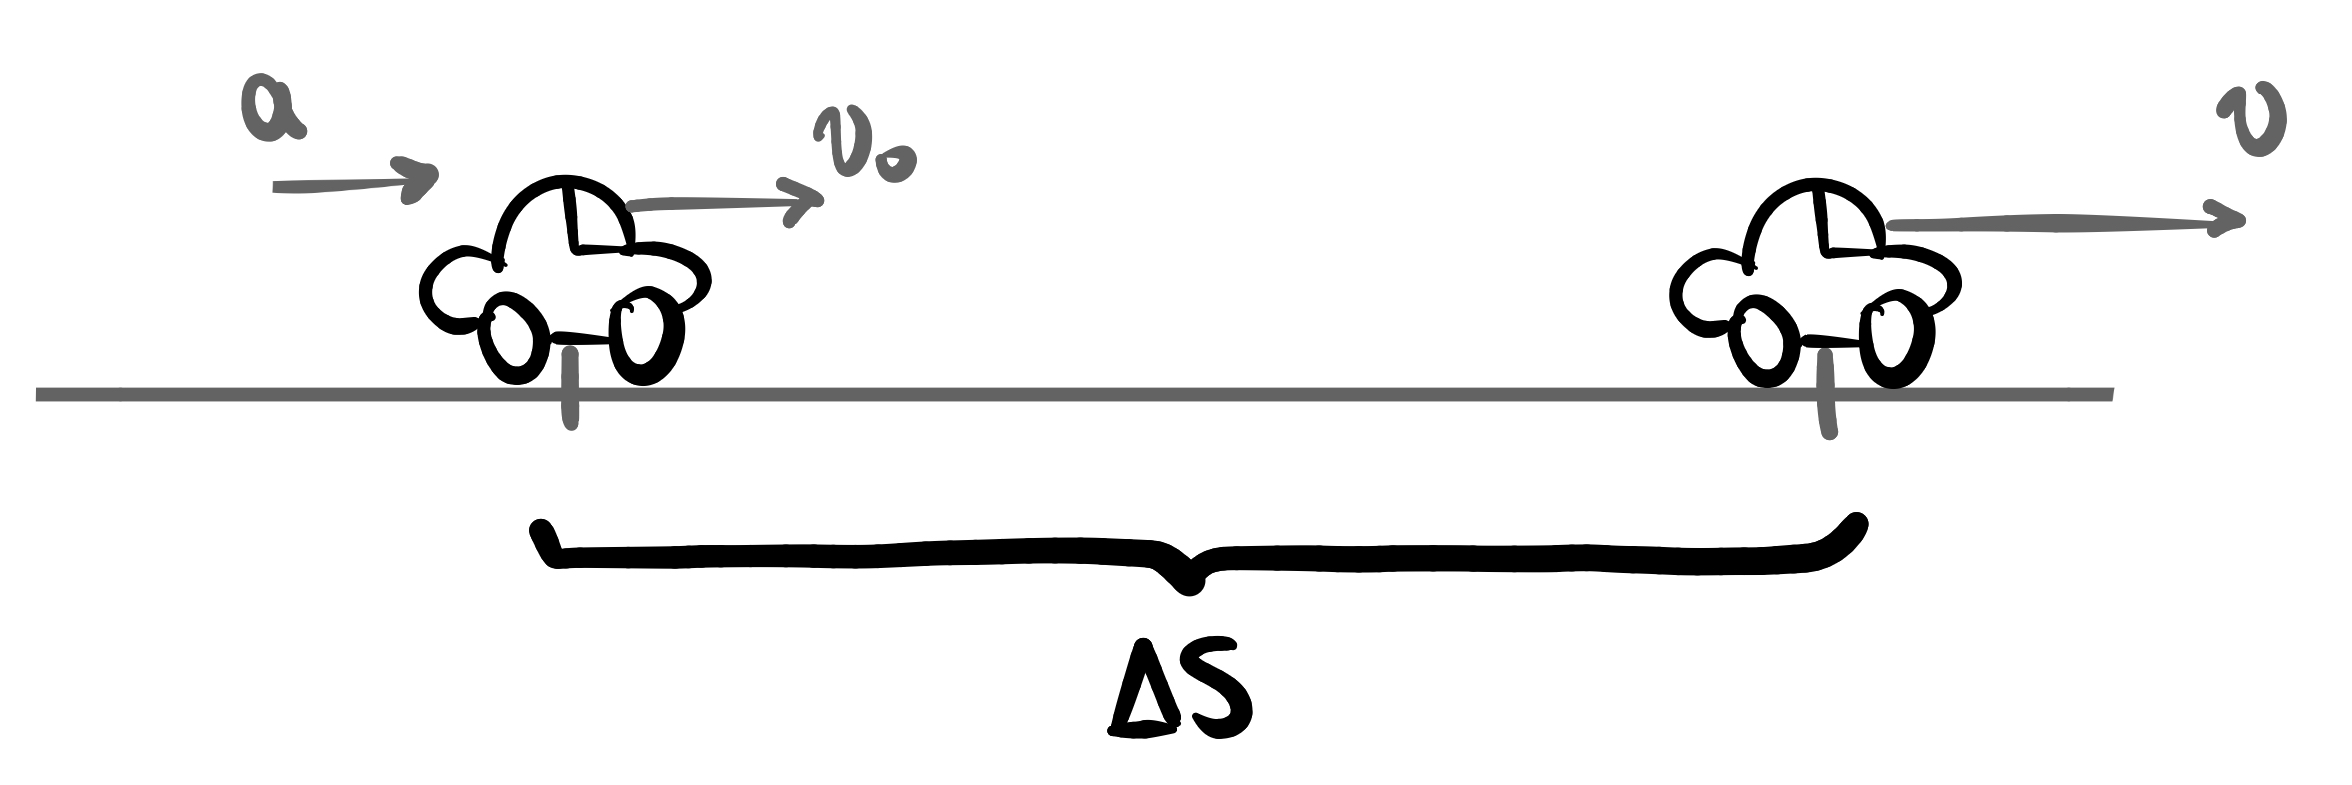
\includegraphics[scale=0.12]{imagensmecanica/torricelli02.jpeg}
    \caption{A construção da Equação de Torricelli.}
    \label{fig_mec_torricelli02}
\end{figure}

Tal equação envolve eliminarmos o tempo como variável para construir uma equação final que não dependa dele. Para tal, considere a Figura \ref{fig_mec_torricelli02}, que mostra um carro em Movimento Uniformemente Variado, com velocidade inicial $v_0$ e uma velocidade final, após um deslocamento $\Delta s$, igual a $v.$ Queremos relacionar essas três grandezas, sem envolver o tempo. Note que, por se tratar de um MUV, ele é governado pelas Equações \eqref{mecanica_eq_muvfuncaoposicao} e \eqref{mecanica_eq_muvfuncaovelocidade}. Podemos eliminar o tempo em uma delas e substituir na outra, a fim de alcançar o que pretendemos. Ou seja, nossos passos são:

\begin{itemize}
    \item [(i)] Usar a função horária da velocidade -- a Equação \eqref{mecanica_eq_muvfuncaovelocidade} -- para eliminar o tempo:

    $$ v = v_0 + at \implies v- v_0 = at \implies \boxed{t = \dfrac{v-v_0}{a} .}$$

     \item [(ii)] Substituímos tal resultado na função horária da posição para o MUV -- a Equação \eqref{mecanica_eq_muvfuncaoposicao} -- a fim de eliminar o tempo:

     \begin{align}
    \Delta s &= v_0t + \dfrac{1}{2}at^2 \nonumber \\
       &= v_0 \left( \dfrac{v-v_0}{a} \right) +\dfrac{1}{2}a \left( \dfrac{v-v_0}{a} \right)^2 \nonumber\\
       &= \dfrac{v_0v-v_0^2}{a} + \dfrac{\cancel{a}}{2} \left( \dfrac{v^2 -2vv_0 + v_0^2}{a^\cancel{2}} \right) \nonumber\\
       &= \dfrac{v^2-v_0^2}{2a}, \nonumber
     \end{align}
      \noindent de onde segue que $v^2 = v_0^2 +2a \Delta s$, como queríamos demonstrar.
\end{itemize}




\secgfe{Onde é usada}

Ela é usada em quaisquer problemas de Cinemática, envolvendo especificamente o Movimento Uniformemente Variado, nos quais não estamos interessados -- ou não temos informação -- a respeito do tempo. Note que, na Equação de Torricelli, o tempo não aparece em nenhum membro da equação. Em tais tipos de problemas, usar tal equação \textbf{não é obrigatório}, mas, em geral, \textbf{encurta e simplifica a resolução do problema}, como veremos no exemplo a seguir.

Considere o problema de se computar o deslocamento sofrido pelo carro da Figura \ref{fig_mec_torricelli} ao longo dos dois instantes registrados.

\begin{figure}[h]
    \centering
    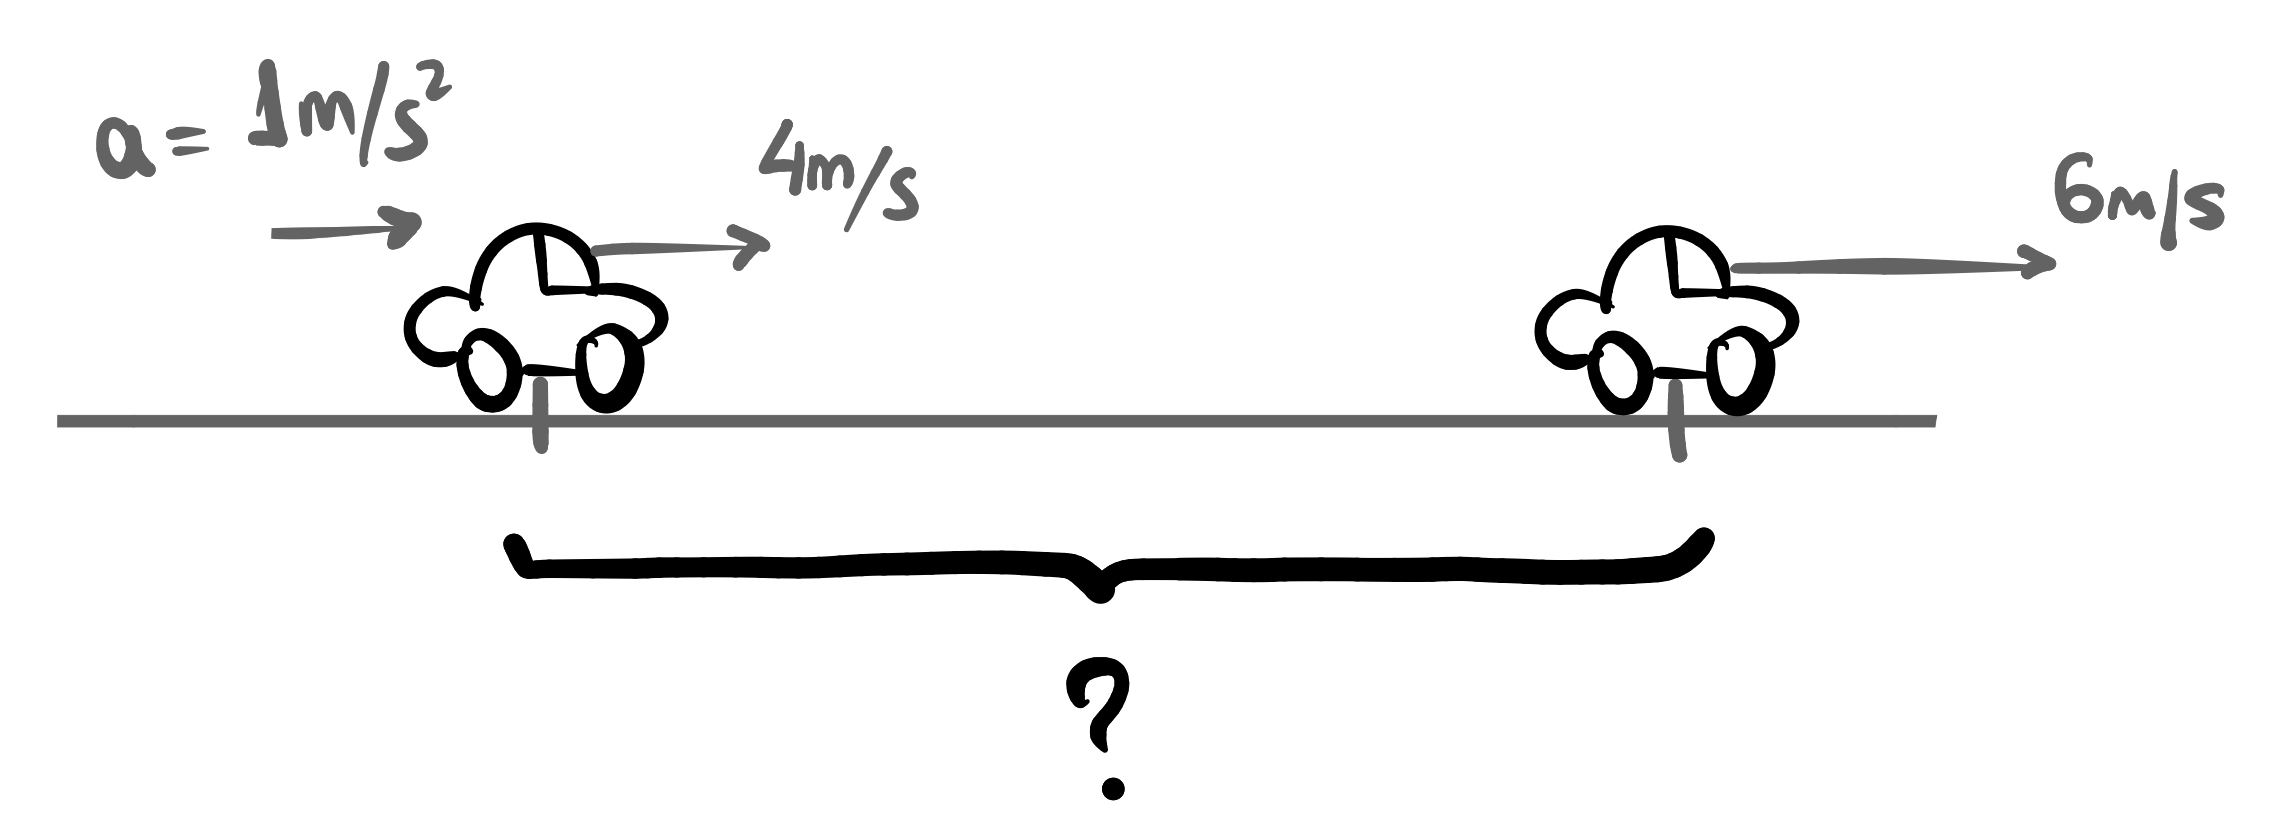
\includegraphics[scale=0.12]{imagensmecanica/torricelli01.jpeg}
    \caption{Construindo uma equação cinemática independente do tempo.}
    \label{fig_mec_torricelli}
\end{figure}

Perceba que não temos nenhuma informação a respeito do tempo que dura tal movimento -- e tampouco estamos interessados em tê-la: queremos saber apenas sobre o deslocamento. Contudo, caso não tivéssemos percebido isso, poderíamos prosseguir, em uma primeira abordagem, da seguinte maneira: como queremos computar o deslocamento, parece mais imediato usar a Equação \eqref{mecanica_eq_muvfuncaoposicao}, que fornece diretamente o valor do deslocamento $\Delta s$ por meio de

$$ \Delta s = v_0t + \dfrac{1}{2}at^2.$$

Contudo, olhando para tal equação, nós sabemos quanto vale a velocidade inicial $v_0$ e a aceleração $a$, porém não sabemos quanto tempo transcorreu desde o instante inicial até o final, no qual a velocidade atinge o valor de 6 m/s. Desse modo, para usar tal equação e resolver o problema, precisaríamos, antes, dar um passo intermediário e computar quanto tempo transcorreu entre aqueles dois instantes. O raciocínio, portanto, ocorreria em duas etapas, como se segue:

\begin{itemize}
    \item [(i)] Cálculo do tempo

    Usamos a Equação \eqref{mecanica_eq_muvfuncaovelocidade} para descobrir quanto tempo se passou entre as duas posições do carro, ou seja:

    $$ v= v
    _0+at \implies 6 = 4+1\cdot t \implies \boxed{t=2s.}$$

    \item [(ii)] Agora, munidos de tal resultado, podemos finalmente usar a Equação \eqref{mecanica_eq_muvfuncaoposicao} e computar o deslocamento que pretendíamos:

    $$ \Delta s = v_0t + \dfrac{1}{2}at^2 \implies \Delta s = 4 \cdot 2 + \dfrac{1}{2}\cdot 1 \cdot 2^2 \implies \boxed{ \Delta s = 10\text{m.}}$$
\end{itemize}

Uma segunda solução para tal problema -- e mais direta, como veremos -- seria o leitor perceber que o tempo não nos interessa, de modo que o passo inicial de computá-lo, como feito na solução anterior, acaba sendo desnecessário. 

Sendo assim, poderíamos usar direto a Equação de Torricelli que, como o leitor viu em sua demonstração, é construída justamente ao eliminar o tempo em uma equação e substituir na outra, ou seja, ela já contém, em seu pressuposto, a eliminação da etapa intermediária de se computar o tempo. Sendo assim, nossa resolução seria:

$$ v^2=v_0^2 + 2a \Delta s \implies 6^2 = 4^2+2 \cdot 1 \cdot \Delta s \implies \boxed{ \Delta s = 10\text{m}.}$$

Chegamos, naturalmente, na mesma resposta, porém realizando menos etapas. Note que, em tal solução, não sabemos quanto tempo durou o movimento -- mas nunca estivemos interessados em sabê-lo, desde o princípio. Por eliminar essa etapa intermediária do cálculo do tempo -- que é a premissa da Equação de Torricelli -- é que tal solução ficou mais curta e objetiva.





\secgfe{Erros comuns}

Os erros mais comuns quanto ao uso dessa equação são dois:

\begin{itemize}
    \item [(i)] Querer usá-la para outros movimentos que não sejam o Movimento Uniformemente Variado. Note que a Equação de Torricelli foi \textbf{construída} a partir das Equações \eqref{mecanica_eq_muvfuncaoposicao} e \eqref{mecanica_eq_muvfuncaovelocidade}, que são equações que \textbf{valem exclusivamente para um objeto que se move com aceleração constante}, ou seja, um objeto que esteja em um Movimento Uniformemente Variado. Logo, por conseguinte, a Equação de Torricelli também só valerá neste regime. 

    Se tentarmos aplicá-la para um corpo que descreve um Movimento Harmônico Simples (que será estudado posteriormente), um movimento com aceleração variável ou qualquer outro tipo de movimento que não seja o MUV, a equação, certamente, fornecerá resultados errados, por não valer em tais regimes.


    \item [(ii)] O sinal da aceleração.

    % Perceba que, ao fazermos a demonstração matemática da Equação \eqref{mecanica_eq_torricelli}, usamos como passo intermediário a equação $v=v_0+at,$ na qual a aceleração e as velocidades possuem o mesmo sinal. Ou seja, partimos da premissa de que o movimento era acelerado.

    % Se fizéssemos a demonstração para um movimento retardado, chegaríamos -- como o leitor pode fazer e verificar por si mesmo -- na equação

    % $$v^2 = v_0^2 - 2 a \Delta s. $$

    % Desse modo, a bem da verdade, teríamos duas equações de Torricelli: uma para o movimento acelerado, que é aquela descrita pela Equação \eqref{mecanica_eq_torricelli}, e uma para o movimento retardado, que é a equação acima. Contudo, essa segmentação parece mais complicar do que facilitar, e, como as duas equações são quase idênticas, a menos de uma troca de sinal, podemos optar por unificar as duas equações e dizer que há apenas uma: aquela descrita pela Equação \eqref{mecanica_eq_torricelli}. 

    % Para que isso seja verdade, basta convencionarmos que em tal equação a aceleração entra com sinal positivo em caso de movimento acelerado e sinal negativo em caso de movimento retardado. Com essa convenção, a equação se ajustará corretamente para cada caso. 

    % Assim, um erro comum é o aluno não se atentar a isso, e usar a aceleração como positiva na Equação \eqref{mecanica_eq_torricelli} para um movimento retardado, ou colocar o sinal negativo, sendo o movimento acelerado.

Perceba que, na demonstração da \eqref{mecanica_eq_torricelli}, usamos como passo intermediário
a Equação \eqref{mecanica_eq_muvfuncaovelocidade}, na qual a aceleração $a$ já carrega o seu sinal: ela é positiva
se aponta no mesmo sentido que o deslocamento, e negativa se aponta no sentido
contrário. Isso não é uma peculiaridade da demonstração --- é exatamente o mesmo
critério de sinal que usamos em toda a Cinemática.

Dito isso, há um erro bastante comum: o estudante identifica, por exemplo, que o
corpo está desacelerando e coloca o valor numérico da aceleração na equação sem sinal, obtendo
%
\begin{equation*}
    v^2 = v_0^2 + 2 \cdot 3 \cdot \Delta s,
\end{equation*}
%
\noindent para uma aceleração de $3$ m/s$^2$, no caso. Quando o correto seria inserir $a = -3\,\text{m/s}^2$, resultando em
%
\begin{equation*}
    v^2 = v_0^2 + 2\cdot(-3)\cdot\Delta s .
\end{equation*}

A regra é simples e a mesma que vale para todas as equações do MUV: defina
um referencial, atribua o sinal correto à aceleração dentro desse referencial, e
insira esse valor --- com sinal --- na Equação de Torricelli. A equação em si é sempre
a mesma; quem diferencia o movimento acelerado do retardado é o sinal de~$a$,
não uma fórmula diferente. De forma prática: movimentos acelerados carregarão aceleração positiva na Equação \eqref{mecanica_eq_torricelli}, enquanto movimentos retardados carregarão acelerações negativas.
    


    
\end{itemize}


\secgfe{Observações}

Cabe aqui uma breve observação sobre unidades de medida: a Equação de Torricelli envolve velocidades, aceleração e deslocamento. Se usarmos todas as grandezas em unidades de medida do SI, a respectiva grandeza calculada também irá ser fornecida em unidades do SI, ou seja:

\begin{itemize}
    \item Se usarmos $v_0$ em m/s, $a$ em m/s$^2$ e $\Delta s$ em m, então a equação irá nos fornecer o valor de $v$ em m/s.

    \item  Se usarmos $v_0$ em m/s, $v$ em m/s e $a$ em m/s$^2$, então a equação irá nos fornecer o valor de $\Delta s$ em m.

    \item Contudo, note que se usarmos $v_0$ em m/s, $v$ em km/h e $\Delta s$ em cm, então o autor há de lhe confessar que não faz a menor ideia de qual será a unidade de medida da aceleração que a equação irá fornecer. Ou seja, atente-se às unidades de medida que você coloca na equação para que o resultado final faça sentido.
    
    \end{itemize}



%Exemplo resolvido

\vspace{0.3cm}

\begin{exemplo}[Nível I]\label{exemplo_cinematicaescalar_torricelliex01}


Um carro, com velocidade inicial de 4 m/s, pisa no freio e imprime uma desaceleração constante de 1 m/s$^2$. Qual é a distância total percorrida por este veículo até parar?


\resolucao


A Figura \ref{fig_mec_torricelli03} ilustra a situação do problema. Note que trata-se de um problema em que não temos informação alguma a respeito do tempo, e tampouco pede-se para computar o tempo. Desse modo, usar a Equação \eqref{mecanica_eq_torricelli} parece ser um bom caminho. Assim, a solução é a que se segue:

$$ v^2=v_0^2 + 2a \Delta s \implies 0^2 = 4^2 +2 \cdot (-1) \cdot \Delta s \implies \boxed{ \Delta s = 8\text{m}.} $$

{
\centering
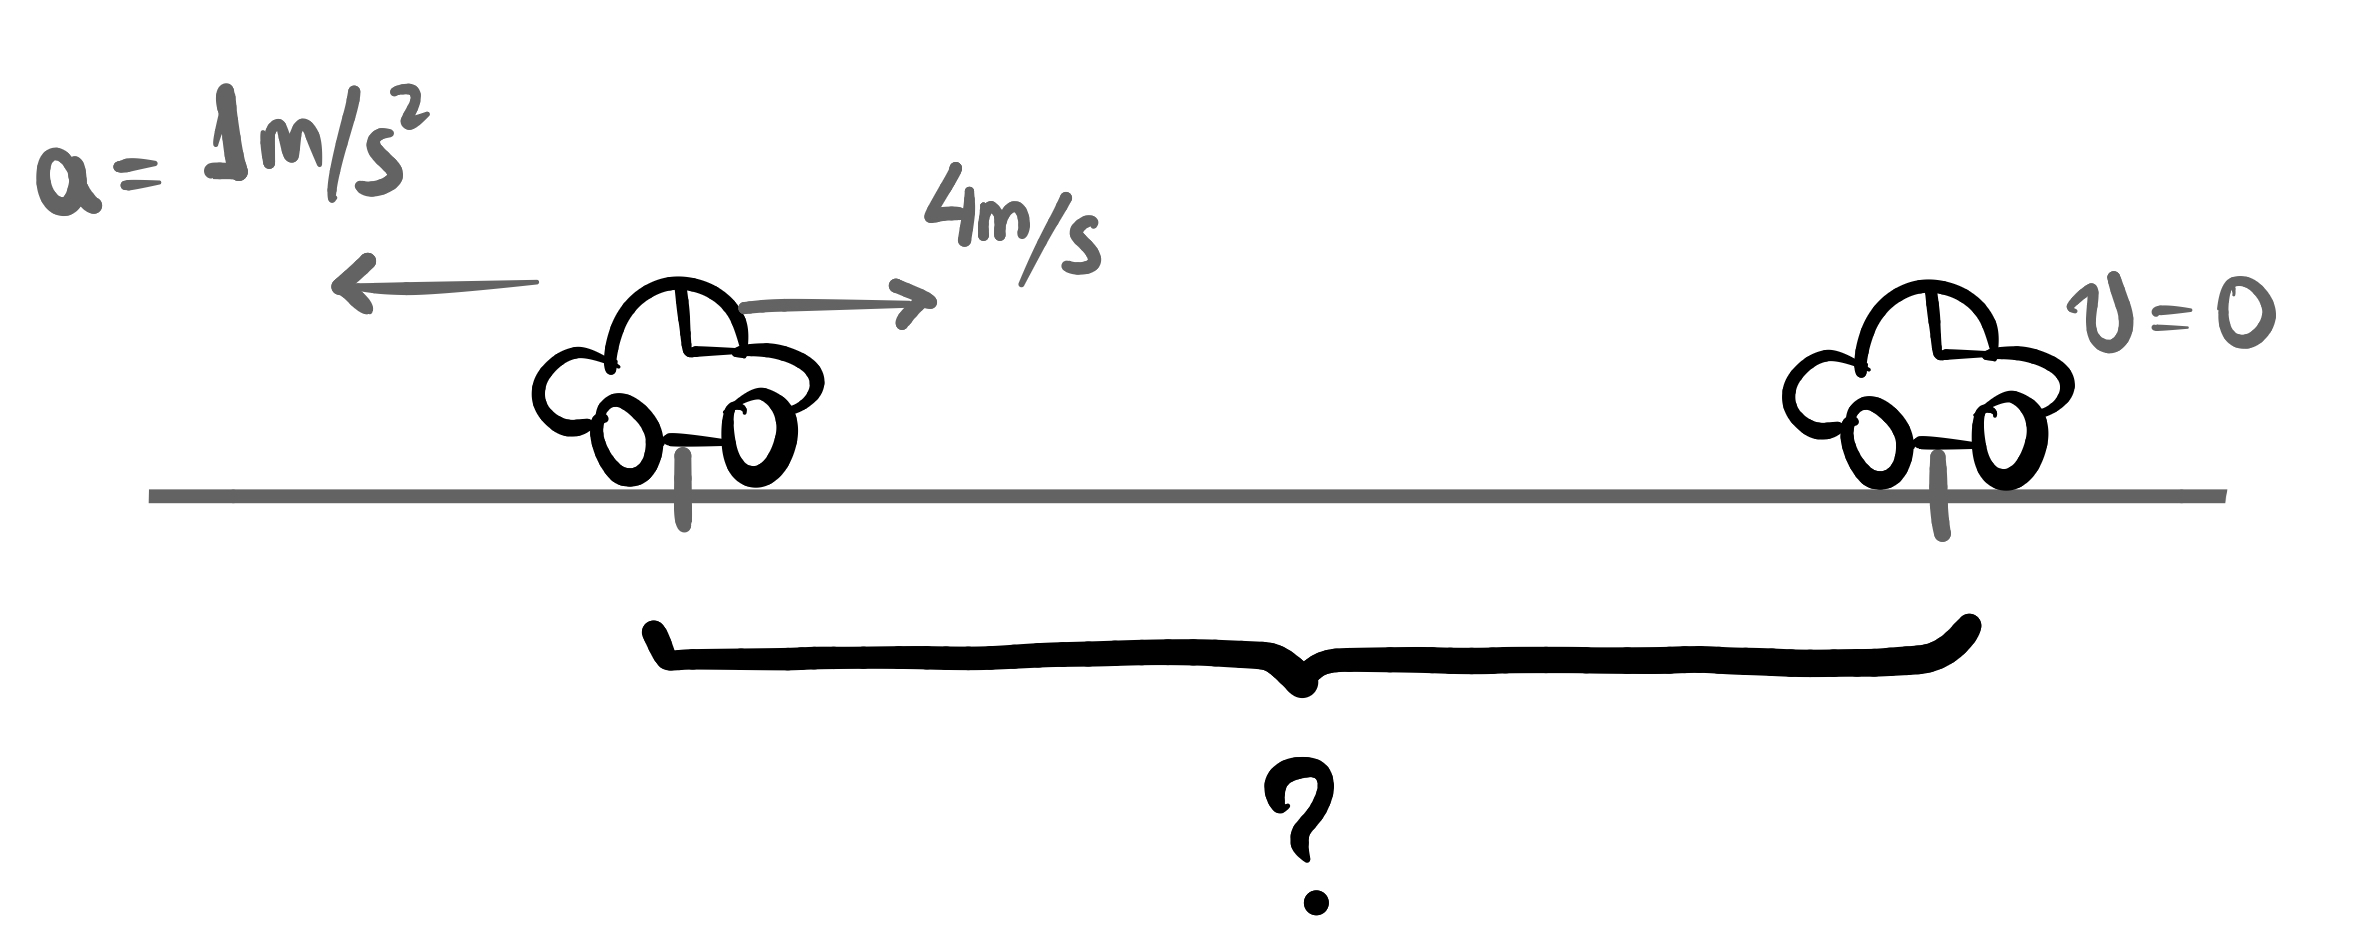
\includegraphics[width=0.5\linewidth]{imagensmecanica/torricelli03.jpeg}
\captionof{figure}{Carro freando com desaceleração constante.}
\label{fig_mec_torricelli03}
} 
\vspace{0.3cm}

Note que usamos a velocidade final $v$ como sendo $0$, uma vez que no instante final o carro estará parado. Além disso, como o movimento é retardado, a aceleração entra com sinal negativo na Equação de Torricelli.

\end{exemplo}

\vspace{0.3cm}







\begin{exemplo}[Nível II]\label{exemplo_cinematicaescalar_torricelliex02}


Dois corpos $A$ e $B$ movem-se ao longo da mesma reta. O corpo $A$ parte do repouso com aceleração constante $a$, enquanto o corpo $B$ parte do repouso, no mesmo instante e mesma posição de $A$, com aceleração constante $2a$. Quando $A$ atinge velocidade $v$ ele alcança uma certa posição. Encontre a velocidade de $B$ quando ele passar por essa mesma posição.


\resolucao


Para chegar na velocidade $v$, saindo do repouso, o corpo $A$ percorre uma distância $\Delta x_A,$ que pode ser obtida pela Equação \eqref{mecanica_eq_torricelli}:

$$ v^2 = \cancelto{0}{v_0^2}+2a \Delta x_A \implies \Delta x_A = \dfrac{v^2}{2a}.$$

Já o corpo $B$, partindo do mesmo ponto que $A,$ passará pela mesma posição que ele quando percorrer a mesma distância $\Delta x_A. $ Logo, sua velocidade $v_B$ nessa posição também pode ser obtida pela Equação \eqref{mecanica_eq_torricelli}:

$$ v_B^2 = \cancelto{0}{v_0^2}+2(2a) \Delta x_A \implies v_B^2 = 4a \dfrac{v^2}{2a} \implies \boxed{v_B = v\sqrt{2}.}$$


\end{exemplo}

\vspace{0.3cm}





% \begin{exemplo}[Nível III]\label{exemplo_cinematicaescalar_torricelliex03}



% Um corpo move-se em linha reta com velocidade inicial $v_0$ e deve ser freado até parar. Você dispõe de duas desacelerações constantes possíveis, de módulos $a_1$ e $a_2$ ($a_1\neq a_2$, ambas positivas). O procedimento de frenagem será o seguinte: primeiro aplica-se a desaceleração $a_1$ até a velocidade cair a $v_1$; em seguida aplica-se $a_2$ até o repouso. Você pode escolher livremente o valor de $v_1$ (isto é, o instante de troca).

% Determine o valor de $v_1$ que minimiza a distância total de frenagem e calcule essa distância mínima.


% \resolucao


% Usaremos a Equação \eqref{mecanica_eq_torricelli} nos dois trechos. Para o primeiro deles, temos:


% \medskip
% \textbf{Trecho 1:} de $v_0$ até $v_1$ com aceleração $-a_1$.
% Pela equação de Torricelli,
% \[
% v_1^2=v_0^2+2(-a_1)s_1
% \quad\implies\quad
% s_1=\frac{v_0^2-v_1^2}{2a_1}.
% \]

% \medskip
% \textbf{Trecho 2:} de $v_1$ até $0$ com aceleração $-a_2$.
% \[
% 0=v_1^2+2(-a_2)s_2
% \quad\implies\quad
% s_2=\frac{v_1^2}{2a_2}.
% \]

% \medskip

% A distância total percorrida até parar completamnete é $s=s_1+s_2$. Logo,
% \[
% s(v_1)= s_1+s_2 =\frac{v_0^2-v_1^2}{2a_1}+\frac{v_1^2}{2a_2}
% =\frac{v_0^2}{2a_1}+v_1^2\left(\frac{1}{2a_2}-\frac{1}{2a_1}\right).
% \]

% Perceba que todos os termos -- exceto $v_1$ -- são constantes e pré-determinados. Nossa função soma um termo que tem um coeficiente multiplicando $v_1^2$. Sendo $v_1^2$ sempre positivo, vamos analisar o sinal do coeficiente que o acompanha. Para tal, defina
% \[
% C=\left(\frac{1}{2a_2}-\frac{1}{2a_1}\right)=\frac{a_1-a_2}{2a_1a_2}.
% \]

% \medskip
% \textbf{Caso 1:} $a_2>a_1$ $\implies C<0$. Nesta caso $s$ diminui quando $v_1^2$ aumenta, já que o termo que contém $v_1^2$ fica sendo subtraído. Logo, o mínimo ocorre para o maior valor possível de $v_1,$ isto é, em $v_1=v_0$:
% \[
% s_{\min}=\frac{v_0^2-v_0^2}{2a_1}+\frac{v_0^2}{2a_2}=\frac{v_0^2}{2a_2}.
% \]

% \medskip
% \textbf{Caso 2:} $a_2<a_1$ $\Rightarrow C>0$. Neste caso $s$ aumenta quando $v_1^2$ aumenta, já que o termo que contém $v_1^2$ está sendo somado. Logo, o mínimo ocorre para o menor valor possível de $v_1$, isto é, em $v_1=0$:
% \[
% s_{\min}=\frac{v_0^2}{2a_1}.
% \]

% Note que, em um primeiro contato, parece um problema difícil, mas na verdade ele é bem fácil: use o maior valor de aceleração disponível e freie com ela durante todo o movimento -- essa é a forma de ter a frenagem mais eficiente e parar o carro na menor distância possível. Razoável, não?


% \end{exemplo}

\begin{exemplo}[Nível III]\label{exemplo_cinematicaescalar_torricelliex03}

Um corpo parte do repouso, acelera uniformemente com aceleração $a_1$ até atingir
velocidade $v_0$, e em seguida desacelera uniformemente com aceleração $a_2$ até
parar. Um segundo corpo parte simultaneamente do mesmo ponto com velocidade
constante $v_c$ e chega ao mesmo destino no mesmo instante. Determine $v_c$ e mostre
que o resultado independe de $a_1$ e $a_2$.

\resolucao

Calculemos o tempo e a distância de cada fase separadamente. Na \textit{fase de
aceleração}, o corpo parte do repouso e atinge $v_0$:

$$ t_1 = \frac{v_0}{a_1}, \qquad d_1 = \frac{v_0^2}{2a_1}. $$

Na \textit{fase de desaceleração}, o corpo parte de $v_0$ e para:

$$ t_2 = \frac{v_0}{a_2}, \qquad d_2 = \frac{v_0^2}{2a_2}. $$

Nos dois casos as distâncias percorridas foram obtidas pela Equação de Torricelli, e o tempo de percurso foi obtido pela Função Horária da Velocidade do MUV. O tempo total e a distância total são, portanto,

$$ T = t_1 + t_2 = v_0\!\left(\frac{1}{a_1}+\frac{1}{a_2}\right)
     = \frac{v_0(a_1+a_2)}{a_1 a_2}, $$

$$ D = d_1 + d_2 = \frac{v_0^2}{2}\!\left(\frac{1}{a_1}+\frac{1}{a_2}\right)
     = \frac{v_0^2(a_1+a_2)}{2\,a_1 a_2}. $$

Note que $D = v_0 T/2$. Logo, a velocidade constante equivalente é

$$ \boxed{v_c = \frac{D}{T} = \frac{v_0}{2}.} $$

O fator $(a_1+a_2)/(a_1 a_2)$ aparece tanto em $D$ quanto em $T$ e se cancela
inteiramente: $v_c$ não depende das acelerações.

Não importa se o corpo acelera devagar e freia bruscamente, ou o contrário --- sua
velocidade média é sempre exatamente metade da velocidade máxima alcançada por ele. Um corpo em movimento
uniforme a $v_0/2$ cobre a mesma distância no mesmo tempo, sempre.

\end{exemplo}
\vspace{0.3cm}




\begin{secnivel}[Velocidade Média no MUV]{II}{Velocidade Média no MUV}
 

  \eqLdois{dem}{mecanica_eq_muvvelocidademedia}{v_m = \dfrac{v_1+v_2}{2}}
  
\end{secnivel}








\secgfe{De onde vem}

Essa equação pode ser obtida de um modo bastante semelhante à construção feita para demonstrar a Equação \eqref{mecanica_eq_muvfuncaoposicao}, fazendo, para tanto, apenas uma pequena consideração.

Para entender tal consideração, observe a imagem da Figura \ref{fig_mec_trapezio01}, que mostra um trapézio, de bases $b$ e $B$ e altura $h.$ Pegando o ponto médio $M$ do quarto lado de tal trapézio, iremos construir, como mostra a segunda parte da figura, dois triângulos retângulos congruentes -- eles terão os três ângulos iguais, o que os faria semelhantes, porém suas hipotenusas possuem o mesmo tamanho, de modo que a razão de semelhança é 1 e, portanto, eles são congruentes. Uma semelhança de triângulos nos leva à conclusão de que a distância do ponto $M$ até o lado de tamanho $h$ é igual à média aritmética das bases do trapézio -- tal segmento é conhecido como base média do trapézio, e está destacado na segunda imagem da Figura \ref{fig_mec_trapezio01}.


\begin{figure}[h]
    \centering
    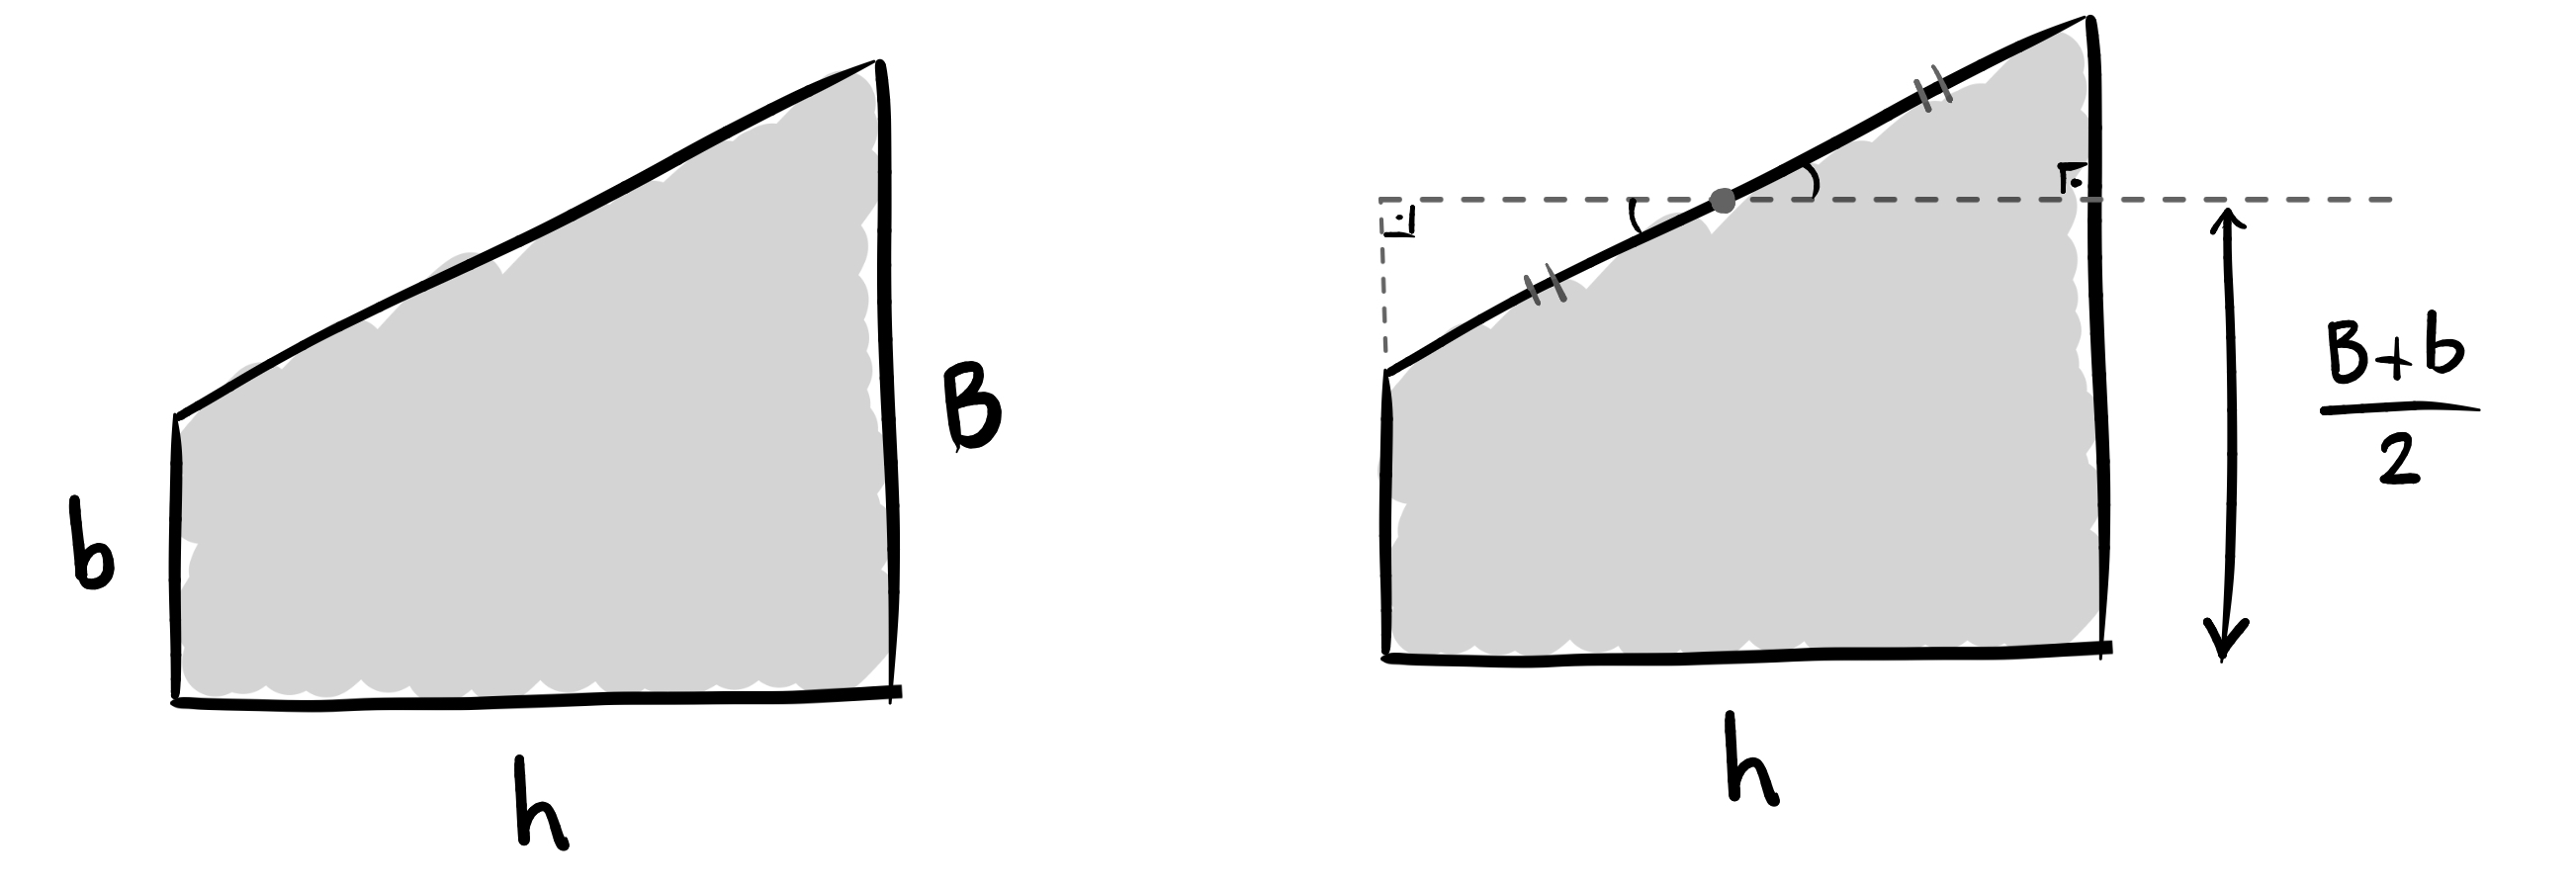
\includegraphics[scale=0.12]{imagensmecanica/muvtrapezio01.jpeg}
    \caption{A base média de um trapézio.}
    \label{fig_mec_trapezio01}
\end{figure}

Note agora que, devido às áreas dos dois triângulos retângulos serem iguais, poderíamos deslocar a área do triângulo do canto superior direito para o triângulo do canto inferior esquerdo. Isso modificaria a nossa figura geométrica sem alterar sua área -- tal processo é o que aparece na Figura \ref{fig_mec_trapezio02}.

Essa construção nos mostra que a área do trapézio de bases $b$, $B$ e altura $h$ é exatamente igual à área do retângulo de altura $\sfrac{(B+b)}{2}$ e altura $h$. Tal retângulo é o que aparece na imagem da direita da Figura \ref{fig_mec_trapezio02}. Ou seja, matematicamente:

$$ \dfrac{(B+b)\cdot h }{2} = \dfrac{(B+b)}{2}\cdot h,$$


\noindent em que o lado esquerdo é a forma tradicional de computar a área de um trapézio e o lado direito é o cálculo tradicional da área de um retângulo, isto é, bases vezes altura.



\begin{figure}[h]
    \centering
    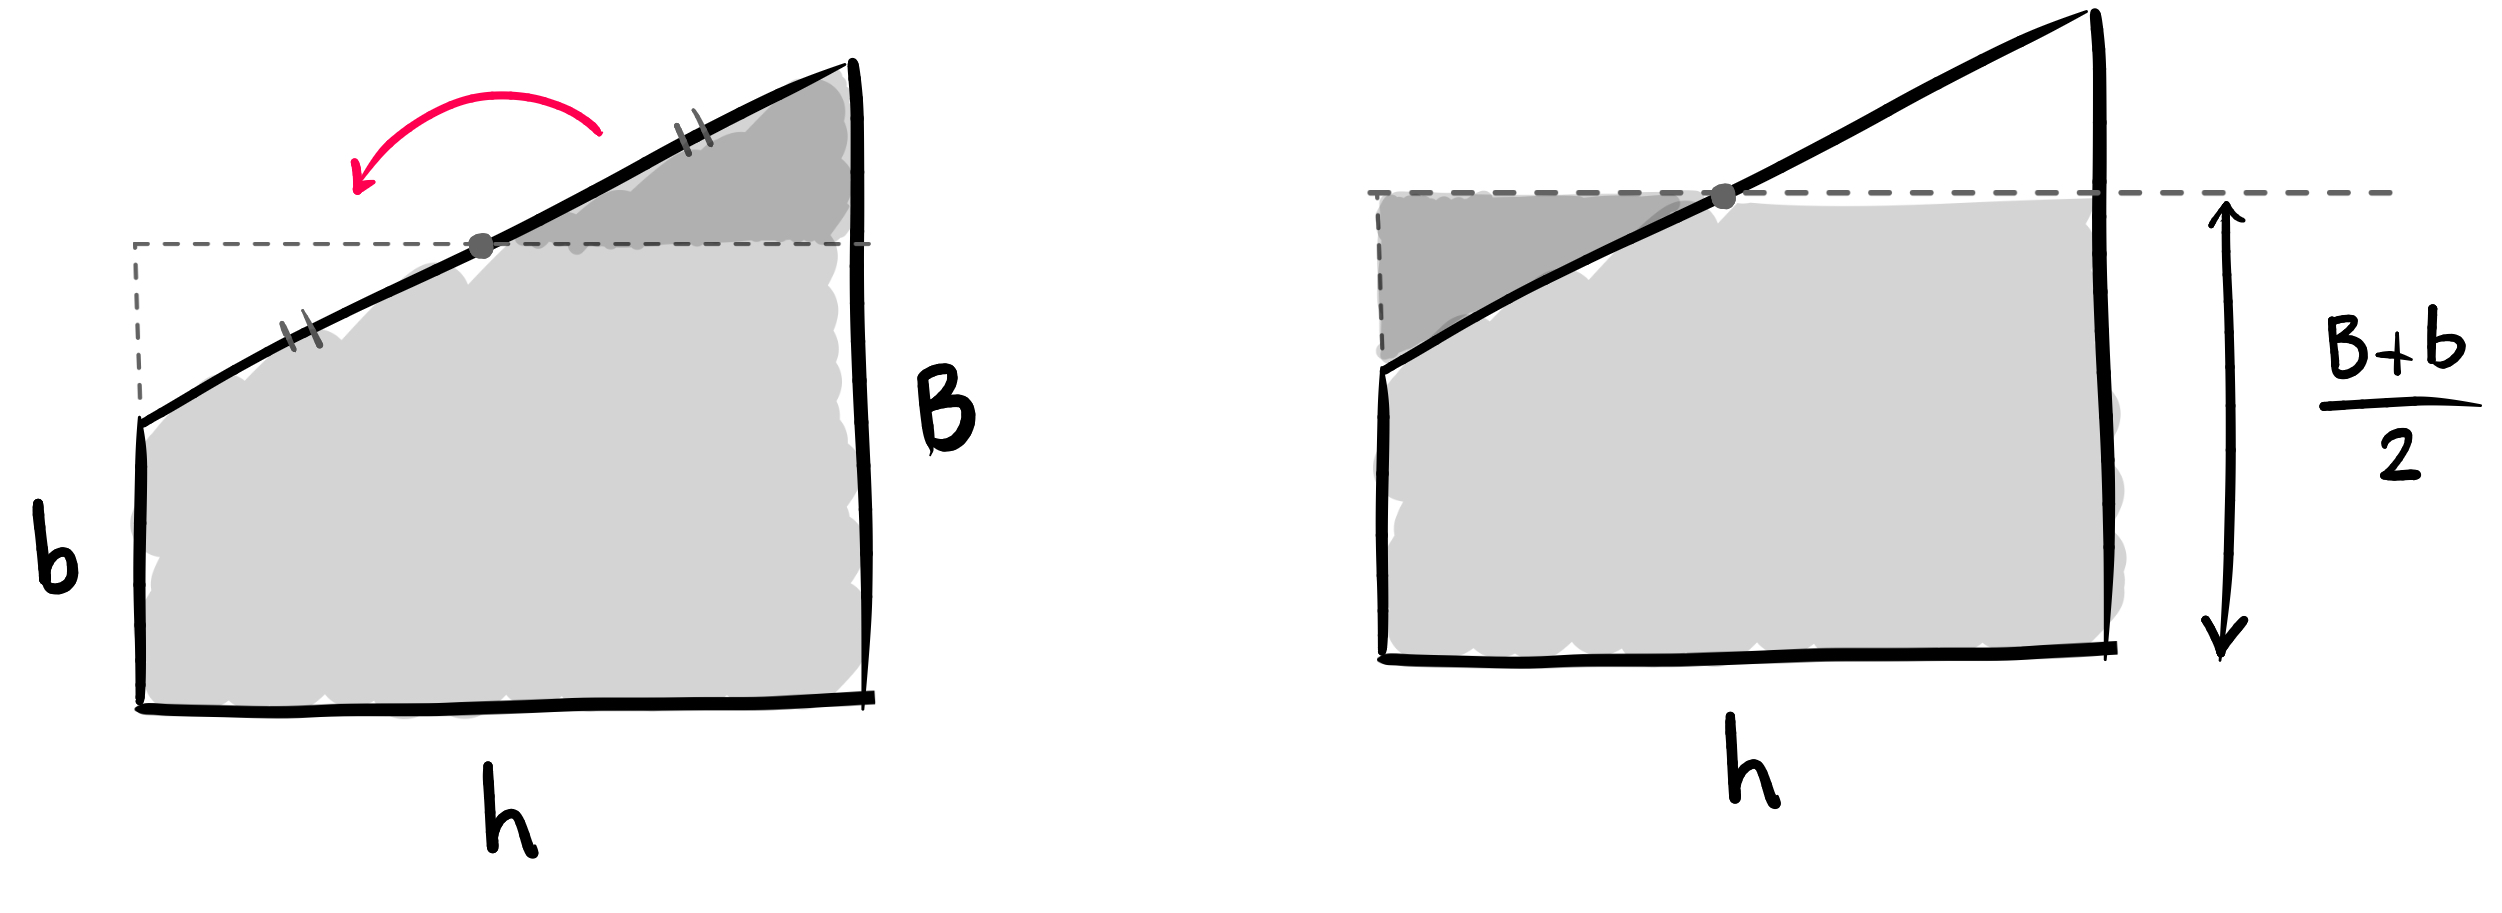
\includegraphics[scale=0.12]{imagensmecanica/muvtrapezio02.jpeg}
    \caption{Modificando a figura sem alterar sua área.}
    \label{fig_mec_trapezio02}
\end{figure}


Dito isso, voltemos agora à construção da Equação \eqref{mecanica_eq_muvfuncaoposicao}, a qual partiu do cálculo da área abaixo do gráfico de velocidade por tempo, destacado na Figura \ref{fig_mec_graficovxt}. Ora, a Figura \ref{fig_mec_trapezio03} evidencia que há duas formas de se calcular tal área: calculando diretamente à área do trapézio, como foi feito na construção da Equação \eqref{mecanica_eq_muvfuncaoposicao}; ou calculando a área do retângulo de mesma altura, porém cuja base é igual à média aritmética das bases do trapézio -- sua base média. 

Neste caso, vemos com clareza que as bases do nosso trapézio são as velocidades inicial $v_0$ e final $v$ do corpo em movimento, de modo que sua base média é 

$$ v'=\dfrac{v_0+v}{2}.$$



\begin{figure}[h]
    \centering
    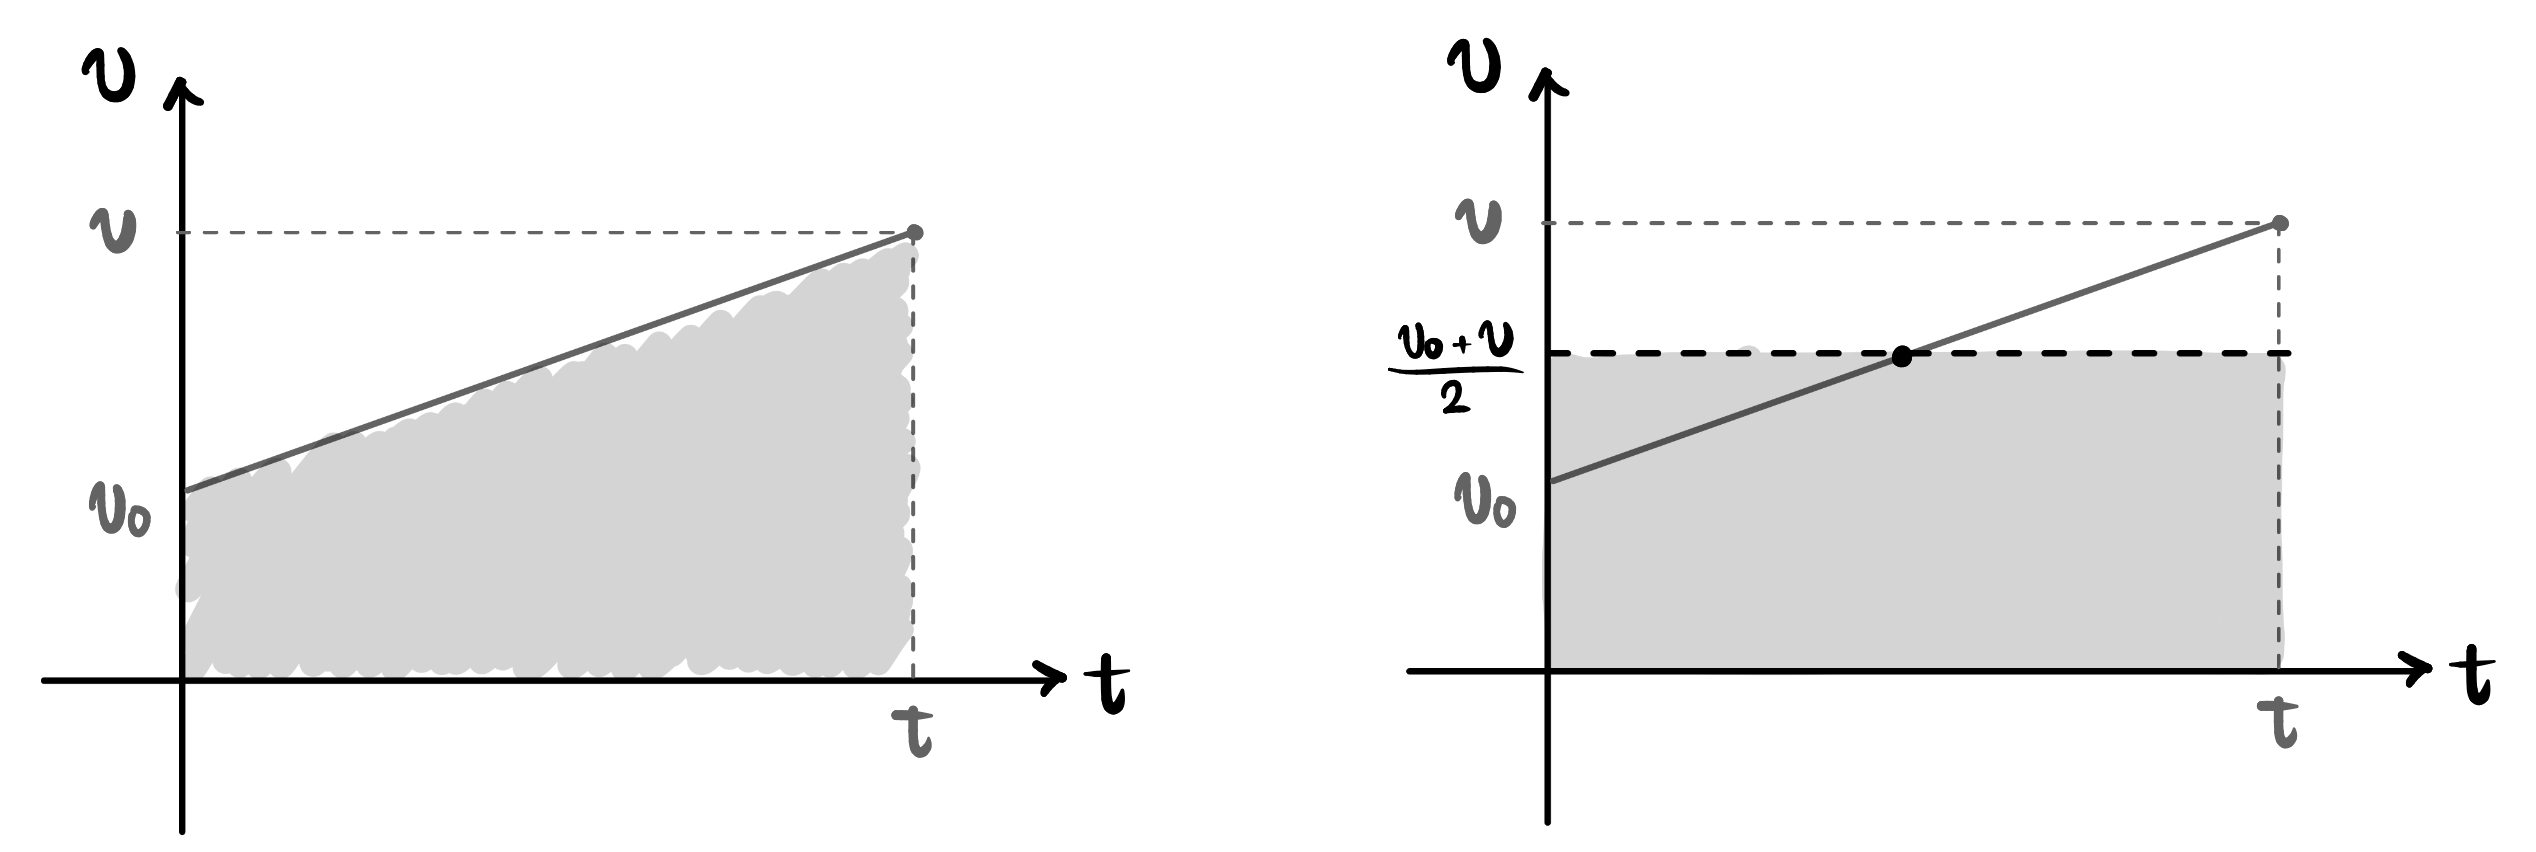
\includegraphics[scale=0.12]{imagensmecanica/muvtrapezio03.jpeg}
    \caption{A equivalência da área do trapézio e do retângulo cuja base é igual à sua base média.}
    \label{fig_mec_trapezio03}
\end{figure}

Ora, se a área abaixo do gráfico é igual ao deslocamento $\Delta s$, podemos computar tal área por meio do retângulo da direita da Figura \ref{fig_mec_trapezio03}:

$$ \Delta s = b \cdot h= \dfrac{(v_0+v)}{2} \cdot t,$$
e, pela definição de velocidade média feita na Equação \eqref{mecanica_eq_velocidademedia}, temos que
$$ \Delta s = v_m \cdot t,$$

\noindent e, igualando as duas últimas equações, chegamos finalmente em

$$ v_m =  \dfrac{(v_0+v)}{2}.$$

Isso quer dizer que, apesar das observações feitas quando definimos a velocidade média -- sendo a principal delas o fato de que calcular a \textbf{velocidade média não é o mesmo que calcular a média das velocidades}, essas duas coisas, curiosamente, coincidem no MUV. É isso que a Equação \eqref{mecanica_eq_muvvelocidademedia} diz: a velocidade média -- exclusivamente no MUV -- em um certo intervalo de tempo é igual à média das velocidades do corpo nos extremos de tal intervalo.

Para deixar absolutamente claro o que fizemos aqui: não estamos dizendo que velocidade média e média aritmética das velocidades são a mesma coisa. Não estamos mudando a definição do conceito de velocidade média -- a velocidade média continua sendo definida pela Equação \eqref{mecanica_eq_velocidademedia}. O que fizemos aqui foi perceber que, exclusivamente para o MUV, a velocidade média, definida exatamente como está na Equação \eqref{mecanica_eq_velocidademedia}, coincide com a média das velocidades.

\secgfe{Onde é usada}

Em problemas de MUV nos quais sabemos a velocidade inicial e final e se deseja calcular o deslocamento ao longo de tal intervalo de tempo, ou então o tempo para que um certo deslocamento ocorra.

É importante o leitor notar que essa equação não introduz nenhuma informação nova na nossa teoria -- ou seja, a princípio, ela é como a Equação de Torricelli: é desnecessária. Não é preciso sabê-la para resolver nenhum problema de MUV, mas, em alguns casos, ela pode ser um bom atalho e encurtar os cálculos, como veremos.


\secgfe{Erros comuns}

Aqui é preciso tomar cuidado, novamente, para não confundir deslocamento com distância. É tentador o leitor pensar que ele pode, agora, simplesmente aplicar a clássica equação $d=vt$ para o MUV, bastando para isso usar $v$ como sendo a média das velocidades. 

Isso está quase correto. Para perceber algumas nuances, voltemos ao contexto do problema descrito na Figura \ref{fig_mec_muvlancamentovertical}. Para os três primeiros segundos de movimento -- a subida -- poderíamos obter a velocidade média da partícula pela média das velocidades, que seria:

$$ v_m=\dfrac{v_0+v}{2}=\dfrac{30+0}{2}=15 \text{m/s}.$$

Assim, a distância percorrida nos três primeiros segundos seria simplesmente

$$d=v_mt=15\cdot 3 = 45 \text{m},$$

\noindent que é exatamente o valor que lá obtivemos, porém aqui de modo bem simples.

Se quiséssemos computar a distância percorrida ao longo dos 6 segundos de movimento poderíamos tentar algo parecido. Primeiro, façamos a velocidade média ao longo dos 6 segundos, que seria a média das velocidades inicial e final ao longo deste intervalo, ou seja:

$$  v_m=\dfrac{v_0+v}{2}=\dfrac{30+(-30)}{2}= 0 \text{m/s}.$$

Parece que ficou estranho. Se optarmos por prosseguir, computaríamos que a distância percorrida neste trecho é

$$ d=v_m t = 0 \cdot 6 = 0 \text{m},$$

\noindent o que está claramente errado.

O erro foi em trocar distância por deslocamento. A equação correta, que vem da definição de velocidade média feita na Equação \eqref{mecanica_eq_velocidademedia}, é que 

$$ \Delta s = v_m \cdot t,$$

\noindent ou seja, o produto da velocidade média pelo tempo fornece o deslocamento, e não a distância. Cabe novamente destacar que, em movimentos cujo sentido não se altera, tais grandezas coincidem. Mas quando há troca de sentido, elas em geral serão diferentes. Perceba que, ao longo dos 6 segundos de movimento da pedra no contexto da Figura \ref{fig_mec_muvlancamentovertical}, a pedra retorna à sua posição inicial, de modo que seu deslocamento total é nulo. Seu deslocamento total sendo zero, naturalmente, sua velocidade média também o será, por definição:

$$ v_m=\dfrac{\Delta s}{\Delta t}= \dfrac{0}{6}=0 \text{m/s,}$$

\noindent o que é condizente com o cálculo obtido pela média das velocidades feito logo acima.


\secgfe{Observações}

Como já pontuamos, a Equação \eqref{mecanica_eq_muvvelocidademedia}, tal como a Equação de Torricelli, não introduz nenhuma informação nova no sistema. Uma forma de ver isso é, inclusive, demonstrando a Equação de Torricelli a partir da Equação \eqref{mecanica_eq_muvvelocidademedia}, o que pode ser feito como se segue:

$$ v_m = \dfrac{v+v_0}{2} = \dfrac{\Delta s}{\Delta t} \implies 2 \Delta s = (v + v_0)t,$$

\noindent e, usando que $v=v_0+at$ podemos escrever que $t=(v-v_0)/a,$ o que nos leva a

$$2 \Delta s = (v + v_0) \dfrac{(v-v_0)}{a} \implies (v+v_0)(v-v_0) = 2a\Delta s \implies v^2 - v_0^2 = 2a \Delta s,$$

\noindent que é a Equação de Torricelli.





%Exemplo resolvido

\vspace{0.3cm}


\begin{exemplo}[Nível I]\label{exemplo_cinematica_muvvelocidademedia01}


Considere um carro que se move com aceleração constante. Sua velocidade, em um certo instante, é de 5 m/s. 10 segundos depois sua velocidade passa a ser de 25 m/s. 

Qual foi a distância percorrida pelo carro neste intervalo de tempo?

\resolucao

Temos, a princípio, três formas de resolver o problema. Façamos todas elas, a título de recapitular todas as equações do assunto e também de deixar claro ao leitor a vantagem de uma em relação à outra.

\begin{itemize}
    \item [(i)] Usando as equações fundamentais do MUV.

    O problema se quebra em duas etapas:

    \begin{enumerate}
        \item Começa-se por computar a aceleração do carro:

        $$ a = \dfrac{\Delta v}{\Delta t}=\dfrac{25-5}{10}=2 \text{m/s$^2$.}$$

        \item Munidos da aceleração, usamos a função horária da posição do MUV -- Equação \eqref{mecanica_eq_muvfuncaoposicao} -- para calcular o deslocamento:

        $$ \Delta s = v_0t + \dfrac{1}{2}at^2 = 5\cdot 10+\dfrac{1}{2}\cdot 2 \cdot 10^2 \implies \boxed{\Delta s =150 \text{m} .}$$
    \end{enumerate}

    \item [(ii)] Usando Torricelli.

    Neste caso, o problema também se divide em duas etapas, sendo a primeira delas a mesma da solução anterior -- o cálculo da aceleração. Munidos de tal valor, vamos à segunda etapa, em que usamos, neste caso, a Equação de Torricelli:

    $$v^2=v_0^2+2a\Delta s \implies 25^2=5^2+2 \cdot 2 \cdot \Delta s \implies \boxed{\Delta s = 150 \text{m}.}$$

    \item [(iii)] Usando o atalho.

    Vimos que, para o MUV, podemos usar $\Delta s=v_m t$ em que $v_m$ é a média das velocidades no intervalo de $0$ a $t$. Ora, a média das velocidades do carro nos instantes extremos do intervalo é

    $$ v_m = \dfrac{v_0+v_f}{2}=\dfrac{25+5}{2}=15 \text{m/s.}$$

    Sendo de $15$ m/s a média das velocidades nestes 10 segundos, a distância percorrida em tal intervalo de tempo é dada por


    $$ d=\Delta s=v_mt=15 \text{m/s}\cdot 10 \text{s} \implies \boxed{d=150 \text{m}.}$$
    
\end{itemize}


    Acredito que o leitor há de concordar que a última solução é a mais eficiente de todas. Apesar de todas as soluções envolverem duas etapas de cálculo, na terceira solução essas etapas são triviais: calcular a média aritmética de dois números e depois multiplicar dois números -- a média das velocidades pelo intervalo de tempo. Tal solução pode ser feita mentalmente, sem haver sequer a necessidade de se armar contas no papel, daí a vantagem de se usar tal equação.

\end{exemplo}

\vspace{0.3cm}







\begin{exemplo}[Nível II]\label{exemplo_cinematica_muvvelocidademedia02}


Um carro parte do repouso e, durante os primeiros $8\,\text{s}$, acelera uniformemente até atingir uma velocidade $v$. Em seguida, mantém essa velocidade constante por $12\,\text{s}$. Sabendo-se que o deslocamento total ao final dos $20\,\text{s}$ é de $400\,\text{m}$, determine o valor de $v$.


\resolucao


Vamos dividir o problema em dois trechos:

\begin{enumerate}
    \item [(i)] MUV, de $0$s a $8$s.

     Podemos computar a velocidade média nesse trecho por meio da média das velocidades, por ser um MUV. Logo:

     $$v_m= \dfrac{v_0+v_f}{2}=\dfrac{0+v}{2}=\dfrac{v}{2},$$

     \noindent o que, junto da definição de velocidade média, nos fornece:

     $$ v_m = \dfrac{\Delta s}{\Delta t} \implies v_m =\dfrac{\Delta s_1}{8} = \dfrac{v}{2} \implies \boxed{\Delta s_1=4v.}$$

     Assim, temos o deslocamento do carro no primeiro trecho, durante sua aceleração.

     \item{(ii)} MU, pelos próximos $12$s.

     Aqui o cálculo é imediato, e o deslocamento do carro é

     $$\Delta s_2 = v \Delta t = v \cdot 12.$$
    
\end{enumerate}


Sendo o deslocamento total de $400$m, temos:

$$ \Delta s_1 + \Delta s_2 = 400 \implies 4v+12v=400 \implies \boxed{v=25 \text{ m/s.}}$$
  

\end{exemplo}

\vspace{0.3cm}






\begin{exemplo}[Nível III (IME-2013)]\label{exemplo_cinematica_muvvelocidademedia03}


Um automóvel percorre uma estrada reta de um ponto $A$ para um ponto $B$. Um radar detecta que o automóvel passou pelo ponto $A$ a $72$ km/h. Se esta velocidade fosse mantida constante, o automóvel chegaria ao ponto $B$ em $10$ min. Entretanto, devido a uma eventualidade ocorrida na metade do caminho entre $A$ e $B$, o motorista foi obrigado a reduzir uniformemente a velocidade até $36$ km/h, levando para isso $20$ s. Restando $1$ min para alcançar o tempo total inicialmente previsto para o percurso, o veículo é acelerado uniformemente até $108$ km/h, levando para isso $22$ s, permanecendo nesta velocidade até chegar ao ponto $B$. O tempo de atraso, em segundos, em relação à previsão inicial, é:
\begin{enumerate}
\item[(a)] $46{,}3$
\item[(b)] $60{,}0$
\item[(c)] $63{,}0$
\item[(d)] $64{,}0$
\item[(e)] $66{,}7$
\end{enumerate}

\resolucao


A distância entre $A$ e $B$ pode ser varrida em $10$ min -- um sexto de hora -- com velocidade constante de $72$ km/h, logo, tal distância vale

$$ d = vt =  \dfrac{72\text{ km}}{\text{ h}} \cdot \dfrac{1 \text{h}}{6} = 12 \text{ km} = 12.000 \text{ m}.$$

Seja um eixo $x$ com origem em $A$ e orientado para $B$. Logo, o problema, ocorrendo na metade do caminho entre $A$ e $B,$ se dá em $x=6000$m e em $t=5$ min (metade do tempo total previsto). Considere agora quatro trechos distintos do movimento:

\begin{enumerate}
    \item [(i)] Desaceleração a partir do meio do caminho.

    Aqui o carro vai de $72$ km/h para $36$ km/h em $20$s, a partir de $x=6.000$m. Sua velocidade média nesse trecho é

    $$ v_m = \dfrac{v_0+v_f}{2} = \dfrac{72+36}{2}=54 \text{ km/h} = 15 \text{ m/s},$$

    \noindent e, pela definição de velocidade média, seu deslocamento foi de

    $$ \Delta s = v_m \Delta t = 15 \cdot 20 = 300 \text{ m}, $$

    \noindent de modo que sua posição passa a ser $x=6.000+300=6300$m em $t=5\text{min} + 20\text{ s}.$


     \item [(ii)] Velocidade constante de $36$ km/h até faltar $1$ min para completar o trajeto.

     Esse trecho se daria até o minuto 9 do movimento. Já tendo se passado 5 minutos e 20 segundos, esse trecho irá durar 3 minutos e 40 segundos, ou 220 segundos. Assim, a distância percorrida aqui é de

     $$ d = v\Delta t= \dfrac{10 \text{ m}}{\text{ s}} \cdot 220 \text{ s} = 2200 \text{ m},$$

     \noindent de modo que a posição do carro agora é $x=6300+2200=8500 \text{ m}.$ Restam, portanto, 60 segundos para completar o tempo inicialmente previsto de 10 minutos e mais $12.000-8.500=3.500 \text{m}$ para serem percorridos.

     


      \item [(iii)] Aceleração quando falta 1 minuto.

       Aqui o carro vai de $36$ km/h para $108$ km/h em $22$s, a partir de $x=8.500$m. Sua velocidade média nesse trecho é

    $$ v_m = \dfrac{v_0+v_f}{2} = \dfrac{36+108}{2}= 72 \text{ km/h} = 20 \text{ m/s},$$

    \noindent e, pela definição de velocidade média, seu deslocamento foi de

    $$ \Delta s = v_m \Delta t = 20 \cdot 22 = 440 \text{ m}, $$

    \noindent de modo que sua posição passa a ser $x=8.500+440=8.940$m em $t=9\text{min} + 22\text{ s},$ de modo que restariam apenas 38 segundos para percorrer o trecho final e não se atrasar.
      

      \item [(iv)] Velocidade constante de $30$ m/s (108 km/h) no trecho final.

      A distância que resta a ser percorrida é de $12.000-8.940=3.060$m, que, com uma velocidade de $30$ m/s, leva um tempo total de 

      $$ t = \dfrac{d}{v} = \dfrac{3060}{30} = 102 \text{ s}.$$

      Como o carro teria apenas $38$ segundos para completar esse trecho, isso gera um tempo de atraso dado por $102-38=64\text{ s,}$ de modo que a resposta correta é a letra D.
\end{enumerate}
  
\end{exemplo}

\vspace{0.3cm}
